\documentclass[a4paper]{article}
\usepackage[T1]{fontenc}
\usepackage{NotesPackage2}
\usepackage{empheq}
% \usepackage[most]{tcolorbox}
\usepackage{slashbox}
\usepackage{subcaption}
\usepackage[version=4]{mhchem}
\usepackage{contour}
\usepackage{blochsphere}
\usepackage{circuitikz}
\usepackage{xspace}
\usepackage{pgfplots}

% Packages used by mathematica
\usepackage{amsmath, amssymb, graphics, setspace}

\usetikzlibrary{calc}
\usetikzlibrary{backgrounds}
\usetikzlibrary{external}
\usetikzlibrary{angles}

\tikzexternalize[prefix=tikz-external/]

\pgfplotsset{compat=1.17}

\author{Willoughby Seago}
\date{September 22, 2020}
\title{Principles of Quantum Mechanics}

% Dirac notation
\renewcommand{\ket}[1]{\vert {#1} \rangle}
\renewcommand{\bra}[1]{\langle {#1} \vert}
\renewcommand{\braket}[2]{\langle {#1} \vert {#2} \rangle}
\renewcommand{\ketbra}[2]{\vert {#1}\rangle\langle {#2} \vert}
\newcommand{\ketResize}[1]{\left| {#1} \right\rangle}
\newcommand{\braResize}[1]{\left\langle {#1} \right\vert}
\newcommand{\braketResize}[2]{\left\langle {#1} \middle\vert {#2} \right\rangle}
\newcommand{\ketbraResize}[2]{\left\vert {#1} \middle\rangle\middle\langle {#2} \right\vert}

% Letters for specific things where a weird font is needed
\newcommand{\hilbert}{\mathcal{H}}
\newcommand{\basis}{\mathcal{B}}
\newcommand{\proj}{\mathcal{P}}
\newcommand{\parity}{\mathscr{P}}
\newcommand{\observable}[1]{\mathcal{#1}}
\newcommand{\complexityClass}[1]{\ensuremath{\mathsf{#1}}\xspace}
\newcommand{\NPcomplexity}{\complexityClass{NP}}
\newcommand{\Pcomplexity}{\complexityClass{P}}
\renewcommand{\order}{\mathcal{O}}
\newcommand{\shannonEntropy}{S_{\mathrm{Sh}}}
\newcommand{\vonNeumannEntropy}{S_{\mathrm{vN}}}
\newcommand{\Efield}{\mathcal{E}}
\newcommand{\Bfield}{\mathcal{B}}
\newcommand{\Pe}{\mathrm{e}}
\newcommand{\Pp}{\mathrm{p}}
\newcommand{\gerade}{\mathrm{g}}
\newcommand{\ungerade}{\mathrm{u}}

% dimensions
\newcommand{\lengthUnit}{\mathrm{length}}
\newcommand{\energyUnit}{\mathrm{energy}}
\newcommand{\timeUnit}{\mathrm{time}}
\newcommand{\massUnit}{\mathrm{mass}}
\newcommand{\momentumUnit}{\mathrm{momentum}}
\DeclareSIUnit{\bitSI}{bit}
\DeclareSIUnit{\bitsSI}{bits}
\DeclareSIUnit{\symbolSI}{symbol} 

% other
\newcommand{\notesVersion}{1.2}
\newcommand{\notesDate}{04/07/2021}
% \renewcommand{\ident}{1}
\newcommand{\st}{\mid}
\newcommand{\tensorProd}{\otimes}
\DeclareMathOperator{\squareIntegrable}{L^2}
\DeclareMathOperator{\Var}{Var}
\newtcbox{\equationBox}[1][]{%
    nobeforeafter, math upper, tcbox raise base,
    enhanced, colframe=lightgray,
    colback=lightgray!25!white, boxrule=1pt,
    #1}
\newcommand{\vecoperator}[1]{\vv{\operator{#1}}}
\newcommand{\eff}{{\mathrm{eff}}}
\newcommand{\spinUp}{\uparrow}
\newcommand{\spinDown}{\downarrow}
\newcommand{\representation}{\mathrel{\rightarrow}}
\DeclareMathOperator{\sign}{sign}
\newcommand{\angmomsquared}[1]{{\tensor{\operator{J}}{^{(#1)}}}^2}
\DeclareSIUnit{\rydberg}{Ry}
\newcommand{\termNotation}[4][]{{#1}\tensor[^{#2}]{\mathrm{{#3}}}{_{#4}}}
\newcommand{\twoVec}[2]{%
    \begin{pmatrix}
        {#1} \\ {#2}
    \end{pmatrix}
}
\newcommand{\twoMat}[4]{%
    \begin{pmatrix}
        {#1} & {#2}\\
        {#3} & {#4}
    \end{pmatrix}
}
\newcommand{\fourVec}[4]{%
    \begin{pmatrix}
        {#1}\\ {#2}\\ {#3}\\ {#4}
    \end{pmatrix}
}
\newcommand{\CNOT}{
    \begin{pmatrix}
        1 & 0 & 0 & 0\\
        0 & 1 & 0 & 0\\
        0 & 0 & 0 & 1\\
        0 & 0 & 1 & 0
    \end{pmatrix}
}
\newcommand{\boltzmann}{k_\mathrm{B}}
\newcommand{\represents}{\mathrel{\leftarrow}}
\newcommand{\union}{\cup}
\newcommand{\intersect}{\cap}
\newcommand{\mean}[1]{\overline{#1}}
\def\centerarc[#1](#2)(#3:#4:#5)% Syntax: [draw options] (center) (initial angle:final angle:radius)
{ \draw[#1] ($(#2)+({#5*cos(#3)},{#5*sin(#3)})$) arc (#3:#4:#5); }

\makeglossaries  % Add glossary entries here
\newacronym{qm}{QM}{quantum mechanics}
\newacronym{pdf}{PDF}{probability density function}
\newacronym{csco}{CSCO}{complete set of commuting/compatible observables}
\newacronym{hup}{HUP}{Heisenberg's uncertainty principle}
\newacronym{tise}{TISE}{time independent Schr\"odinger equation}
\newacronym{stm}{STM}{scanning tunnelling microscope}
\newacronym{tdse}{TDSE}{time dependent Schr\"odinger equation}
\newacronym{qed}{QED}{quantum electrodynamics}
\newacronym{epr}{EPR}{Einstein--Podolsky--Rosen}
\newacronym{cm}{CM}{centre of mass}
\newacronym{lcao}{LCAO}{linear combinations of atomic orbitals}

%\theoremstyle{definition}
%\newtheorem{postulate}{Postulate}
%\declaretheorem[name=Postulate, style=definition]{postulate}
\newcounter{postulateCounter}
\newtcbtheorem[use counter=postulateCounter]{postulate}{Postulate}{colback=green!5, colframe=green!50!black, fonttitle=\bfseries, breakable, description delimiters parenthesis, separator sign none}{pos}

\tcbset{highlight math style={}}

\includeonly{parts/states, parts/observables, parts/dynamics, parts/angular_momentum, parts/recap, parts/approximation_methods, parts/applications_of_quantum_theory}

\begin{document}
    \pagenumbering{roman}  % Number contents pages and glossaries with roman numerals
    \maketitle
    These are my notes for the \textit{principles of quantum mechanics} course from the University of Edinburgh as part of the third year of the theoretical physics degree.
    When I took this course in the 2020/21 academic year it was taught by Professor Luigi Del Debbio\footnote{\url{https://www.ph.ed.ac.uk/people/luigi-del-debbio}} and Professor Arjun Berera\footnote{\url{https://www.ph.ed.ac.uk/people/arjun-berera}}.
    These notes are based on the lectures delivered as part of this course, and the notes provided as part of this course, which are in the process of being published as a textbook.
    The content within is correct to the best of my knowledge but if you find a mistake or just disagree with something or think it could be improved please let me know.
    
    These notes were produced using \LaTeX\footnote{\url{https://www.latex-project.org/}}.
    Graphs where plotted using Python\footnote{\url{https://www.python.org/}}, Matplotlib\footnote{\url{https://matplotlib.org/}}, NumPy\footnote{\url{https://numpy.org/}}, and SciPy\footnote{\url{https://scipy.org/scipylib/}}.
    Diagrams were drawn with tikz\footnote{\url{https://www.ctan.org/pkg/pgf}}.
    
    This is version \notesVersion~of these notes, which is up to date as of \notesDate.
    \begin{flushright}
        Willoughby Seago
        
        s1824487@ed.ac.uk
    \end{flushright}
    \clearpage
    \tableofcontents
    \listoffigures
    \listoftables
    \printglossary[type=\acronymtype, title=Acronyms, style=long]
    \clearpage
    \pagenumbering{arabic}  % Number rest of document with numbers
    \begingroup
    \let\clearpage\relax  % "\begingroup, \let\clearpage\relax, \endgroup" stops automatic pagebreaks after each include
    \part{States}
    \section{Quantum States}
    \subsection{Classical States}
    In classical mechanics a point like system's state is entirely described by two 3-dimensional vectors, namely position, \(\vv x\), and momentum, \(\vv p\).
    These are 3-dimensional real vectors living in \(\reals^3\).
    We can instead view the object \((\vv x, \vv p)\) as a 6-dimensional real vector living in \(\reals^6\).
    In this way we can completely describe the state of the system with one 6-dimensional vector.
    By this we mean that using \((\vv x, \vv p)\) and Newton's laws we can compute the time evolution of the system, that is what the state will be at some time in the future, or what the state was at some time in the past.
    We can also compute other values such as energy and angular momentum, these are observables that we can measure along with position and momentum.
    
    \subsection{Quantum States}
    In \acrfull{qm} the state of a system can also be encoded in a single vector, although the way that we do this is more complex (literally).
    We start with the following postulate:
    \begin{postulate}{}{quantum state is complex vector}
        The state of a quantum system is described by a complex vector.
    \end{postulate}
    In classical mechanics the state vector is real and therefore composed of values that can be measured.
    In \acrshort{qm} we cannot directly measure the components of this complex vector.
    The way we measure observables will be covered in detail later.
    For now we focus on the mathematical side of this statement.
    
    In this course we will use Dirac notation in which a vector is represented by \(\ket{v}\), called a \define{ket}, where \(v\) is some label.
    For example we may use \(\ket{v}\), \(\ket{\uparrow}\), or \(\ket{n, m}\).
    Here \(v\), \(\uparrow\), and \(n, m\) are simply whatever label is best suited to the problem at hand.
    
    \subsubsection{Vector Spaces}\label{sec:vector spaces}
    Our intuition for what is a vector is normally that it is some object with magnitude and direction.
    This definition fails when it comes to complex vectors and is not very useful for vectors of more than 3-dimensions.
    To be mathematically precise a \define{vector} is any element of a vector space, \(\hilbert\).
    This simply moves the problem on to the next definition, what is a vector space?
    
    A \define{vector space}, \((\hilbert, \mathbb{F}, +, \cdot)\), over a field, \(\mathbb{F}\), is a set, \(\hilbert\) and two operations, \(+\) and \(\cdot\).
    We will restrict ourselves to \(\mathbb{F} = \reals, \complex\).
    In the former case we get a real vector space and in the later a complex vector space.
    These operations are
    \begin{itemize}
        \item Vector addition, \({+}\colon\hilbert\times\hilbert\to\hilbert\), which takes two vectors, \(\ket{u}, \ket{v}\in\hilbert\) and maps them to a third vector \(\ket{u} + \ket{v}\in\hilbert\).
        \item Scalar multiplication, \({\cdot}\colon\mathbb{F}\times\hilbert\to\hilbert\), which takes a vector, \(\ket{v}\in\hilbert\), and a scalar, \(\lambda\in\mathbb{F}\), and maps them to a second vector \(\lambda\ket{v}\).
    \end{itemize}
    These operations must satisfy the following properties:
    \begin{itemize}
        \item Associativity of vector addition -- For all \(\ket{u}, \ket{v}, \ket{w}\in\hilbert\)
        \[\ket{u} + (\ket{v} + \ket{w}) = (\ket{u} + \ket{v}) + \ket{w}.\]
        In other words the bracketing around vector addition doesn't matter, the result is the same however it is bracketed.
        This is true for more than three terms being added as well.
        \item Commutativity of vector addition -- For all \(\ket{u}, \ket{v}\in\hilbert\)
        \[\ket{u} + \ket{v} = \ket{v} + \ket{u}.\]
        In other words the order of terms in a sum doesn't matter, the result is the same either way.
        \item Existence of an additive identity -- There exists \(\ket{0}\in\hilbert\) such that 
        \[\ket{0} + \ket{v} = \ket{v}\]
        for all \(\ket{v}\in\hilbert\).
        \(\ket{0}\) is called the zero vector.
        Be careful as \(\ket{0}\) may not always denote the zero vector, for example, if we use \(\ket{p}\) to denote a state with momentum \(p\) then \(\ket{0}\) denotes a state with no momentum.
        This doesn't mean that this is the zero vector.
        \item Existence of additive inverses -- For all \(\ket{v}\) there exists \(-\ket{v}\in\hilbert\) such that
        \[\ket{v} + (-\ket{v}) = \ket{0}\]
        where \(\ket{0}\) is the zero vector.
        We normally shorten this to
        \[\ket{v} - \ket{v} = \ket{0}.\]
        \item Compatibility of scalar and field multiplication -- for all \(\lambda, \mu\in\mathbb{F}\) and \(\ket{v}\in\hilbert\) we have
        \[(\lambda\mu)\ket{v} = \lambda(\mu\ket{v})\]
        here the product \(\lambda\mu\) is computed using multiplication as defined in \(\mathbb{F}\) and \(\mu\ket{v}\) and \(\lambda(\mu\ket{v})\) are computed using scalar multiplication as defined for our vector space.
        \item Identity of scalar multiplication -- If \(1\in\mathbb{F}\) is the multiplicative identity of \(\mathbb{F}\) then
        \[1\ket{v} = \ket{v}\]
        for all \(\ket{v}\in\hilbert\).
        \item Distributivity of scalar multiplication over vector addition -- For all \(\ket{u}, \ket{v}\in\hilbert\) and \(\lambda\in\mathbb{F}\)
        \[\lambda(\ket{u} + \ket{v}) = \lambda\ket{u} + \lambda\ket{v}.\]
        \item Distributivity of scalar multiplication over field addition -- For all \(\lambda, \mu\in\mathbb{F}\) and \(\ket{v}\in\hilbert\)
        \[(\lambda + \mu)\ket{v} = \lambda\ket{v} + \mu\ket{v}.\]
    \end{itemize}
    The important take away here is that for a complex vector space, \(\hilbert\) if \(\ket{u}, \ket{v}\in\hilbert\) and \(\alpha, \beta\in\complex\) then
    \[\alpha\ket{u} + \beta\ket{v} \in \hilbert.\]
    That is \(\hilbert\) is closed under vector addition and scalar multiplication.
    This easily generalises to \(\ket{v_i}\in\hilbert\) and \(\alpha_i\in\hilbert\) so
    \[\sum_i\alpha_i\ket{v_i}\in\hilbert\]
    Any linear combination of vectors is again a vector.
    
    \begin{example}
        Let \(\ket{u}\) and \(\ket{v}\) be vectors with two complex components:
        \[
            \ket{u} =
            \begin{pmatrix}
                u_1\\ u_2
            \end{pmatrix}
            ,\qquad\text{and}\qquad\ket{v} = 
            \begin{pmatrix}
                v_1\\ v_2
            \end{pmatrix}
        \]
        where \(u_1, u_2, v_1, v_2\in\complex\).
        If we define the sum of these two vectors to be
        \[
            \ket{u} + \ket{v} = 
            \begin{pmatrix}
                u_1 + v_1\\ u_2 + v_2
            \end{pmatrix}
            .
        \]
        The addition on the left hand side is vector addition, the addition on the right hand side is field addition in \(\complex\).
        We define scalar multiplication by \(\lambda\in\complex\) as
        \[
            \lambda\ket{v} =
            \begin{pmatrix}
                \lambda v_1\\ \lambda v_2
            \end{pmatrix}
            .
        \]
        Multiplication on the left hand side is scalar multiplication, multiplication on the right hand side is field multiplication in \(\complex\).
        The set, \(\complex^2\), of all such objects with this definition of vector addition and scalar multiplications is a complex vector space.
        We will use this throughout this section to give examples.
    \end{example}
    The fact that a linear combination of vectors is again a vector means that a linear combination of quantum states is again a quantum state.
    This is called the \define{superposition principle}.
    It is a direct consequence of postulate~\ref{pos:quantum state is complex vector} and the closure of vector spaces under addition and multiplication.
    In fact it is possible to state the superposition principle as the first postulate and then derive that the states need to be elements of a vector space.
    
    \subsubsection{Scalar Products}
    The scalar product, or inner product, is a function:
    \begin{align*}
        \cdot\colon\hilbert\times\hilbert &\to \complex\\
        \ket{u}, \ket{v} &\mapsto \braket{u}{v} = z\in\complex.
    \end{align*}
    The inner product also satisfies the following two properties:
    \begin{itemize}
        \item Conjugate symmetry -- For all \(\ket{u}, \ket{v}\in\hilbert\)
        \[\braket{u}{v} = \braket{v}{u}^*\]
        where \(^*\) denotes complex conjugation.
        \item Linearity in the second argument -- For all \(\ket{u}, \ket{v}, \ket{w}\in\hilbert\) and \(\alpha, \beta\in\complex\)
        \[\bra{u}\left[\alpha\ket{v} + \beta\ket{w}\right] = \alpha\braket{u}{v} + \beta\braket{u}{w}.\]
    \end{itemize}
    Combining these properties we get that for all \(\ket{u}, \ket{v}, \ket{w}\in\hilbert\) and \(\alpha, \beta\in\complex\)
    \[\left[\alpha\bra{u} + \beta\bra{v}\right]\ket{w} = \alpha^*\braket{u}{w} + \beta^*\braket{v}{w}.\]
    A vector space equipped with an inner product is called a \define{Hilbert space}.\footnote{Technically it is just an inner product space, a Hilbert space is then an inner product space that is Cauchy complete. That is all series of vectors that converge absolutely (the sum of the norms of the vectors converges) in \(\hilbert\) converge (the sum of the vectors converges) in \(\hilbert\). However all inner product spaces can be extended to be Hilbert spaces so the distinction isn't important for our purposes.}
    \begin{example}
        Given two vectors \(\ket{u}, \ket{v}\in\complex^2\) defined as
        \[
            \ket{u} =
            \begin{pmatrix}
                u_1\\ u_2
            \end{pmatrix}
            ,\qquad\text{and}\qquad\ket{v} = 
            \begin{pmatrix}
                v_1\\ v_2
            \end{pmatrix}
        \]
        the following is a valid inner product:
        \[\braket{u}{v} = u_1^*v_1 + u_2^*v_2.\]
    \end{example}
    
    \subsubsection{Linear Functionals}
    A \define{linear functional} is a function, \(f\), defined on \(\hilbert\) that associates each vector with a complex number,
    \begin{align*}
        f\colon\hilbert &\to \complex\\
        \ket{v} &\mapsto f(\ket{v}) = z\in\complex,
    \end{align*}
    in such a way that
    \[f(\alpha\ket{u} + \beta\ket{v}) = \alpha f(\ket{u}) + \beta f(\ket{v})\]
    for all \(\ket{u}, \ket{v}\in\hilbert\), and \(\alpha, \beta\in\complex\).
    
    For a given vector, \(\ket{u}\in\hilbert\), we can define a linear functional, \(f_{\ket{u}}\) that takes a vector \(\ket{v}\in\hilbert\) and returns a complex number through the correspondence
    \[\ket{v} \mapsto z = f_{\ket{u}}(\ket{v}) = \braket{u}{v}.\]
    It can be shown that all bounded linear functionals that act on \(\hilbert\) can actually be represented like this.
    That is that for any linear functional defined there exists \(\ket{u}\in\hilbert\) such that the linear functional is equivalent to an inner product with this vector.
    This is called the \define{Riesz theorem}.
    This means that given any linear functional we can identify it with a vector and vice versa.
    This one-to-one correspondence led Dirac to introduce the \define{bra} notation where a linear functional is denoted \(\bra{u}\).
    Again \(u\) is just a label and this represents the linear functional \(f_{\ket{u}}\) that has the result of \(f_{\ket{u}}(\ket{v}) = \braket{u}{v}\).
    The space of all linear functionals is called the \define{dual} of the vector space \(\hilbert\), and is denoted \(\hilbert^*\).
    
    \subsubsection{Norms}
    The \define{norm} of a vector is a function:
    \begin{align*}
        \norm{\cdot}\colon\hilbert&\to\reals\\
        \ket{v} &\mapsto \norm{v}
    \end{align*}
    where \(\norm{v}\) has some restraints:
    \begin{itemize}
        \item The triangle inequality -- For all \(\ket{u}, \ket{v}\in\hilbert\)
        \[\norm{\ket{u} + \ket{v}} \le \norm{u} + \norm{v}.\]
        \item Absolutely scaleable -- For all \(\ket{v}\in\hilbert\), \(\lambda\in\complex\):
        \[\norm{a\ket{v}} = \abs{\lambda}\norm{v}.\]
        \item Positive definite -- If \(\norm{v} = 0\) then \(\ket{v} = \ket{0}\) is the zero vector.
    \end{itemize}
    Note that we use \(\norm{\cdot}\) for the norm and \(\abs{\cdot}\) for the absolute value of a complex number defined as \(\abs{z} = \sqrt{z^*z}\).
    This actually hints at the most common norm that we will use throughout this course.
    The norm induced by the inner product is
    \[\norm{v} = \sqrt{\braket{v}{v}}.\]
    Using the fact that the inner product is linear we have \(\braket{v}{v} = \braket{v}{v}^*\) so we know that \(\braket{v}{v}\in\reals\).
    
    In \acrshort{qm} it is conventional to have all state vectors have unital norm.
    The reason for this will become clear when we start to discuss how the physics is extracted from the state vector.
    Fortunately all states can be normalised such that their norm is 1,
    for all \(\ket{v}\in\hilbert\) if \(\norm{v}\ne 0\) then
    \[\frac{1}{\sqrt{\braket{v}{v}}}\ket{v} = \frac{1}{\norm{v}}\ket{v}\]
    is a vector with norm 1.
    This follows from the absolute scaleability and positive definiteness of the norm:
    \[\norm{\frac{1}{\norm{v}}\ket{v}} = \abs{\frac{1}{\norm{v}}}\norm{v} = \frac{1}{\norm{v}}\norm{v} = 1.\]
    Note that if \(\norm{v} = 1\) then
    \[\norm{e^{i\vartheta}\ket{v}} = \abs{e^{i\vartheta}}\norm{v} = 1\cdot 1 = 1.\]
    Thus quantum states are actually only unique up to a factor of \(e^{i\vartheta}\), called the phase.
    \begin{example}
        Let \(\ket{v}\in\complex^2\) be defined by
        \[
            \ket{v} = 
            \begin{pmatrix}
                v_1\\ v_2
            \end{pmatrix}
        \]
        then the norm of \(\ket{v}\) is
        \[\norm{v} = \sqrt{\braket{v}{v}} = \sqrt{v_1^*v_1 + v_2^*v_2} = \sqrt{\abs{v_1}^2 + \abs{v_2}^2}.\]
        We can see how similar this is to the Euclidean norm that we are all used to.
        Also it is clearly only \(0\) if \(v_1, v_2 = 0\), i.e. \(\ket{v} = 0\).
    \end{example}
    
    \subsubsection{Orthogonality}
    Two vectors, \(\ket{u}, \ket{v}\in\hilbert\) are \define{orthogonal} if and only if
    \[\braket{u}{v} = 0.\]
    
    \subsubsection{Operators}
    \define{Operators} are functions:
    \begin{align*}
        \operator{O}\colon\hilbert &\to \hilbert\\
        \ket{v} &\mapsto \operator{O}\ket{v} = \ket{w}\in\hilbert.
    \end{align*}
    An operator, \(\operator{O}\), is a linear operator if for all \(\ket{u}, \ket{v}\in\hilbert\) and \(\alpha, \beta\in\hilbert\)
    \[\operator{O}\left[\alpha\ket{u} + \beta\ket{v}\right] = \alpha\operator{O}\ket{u} + \beta\operator{O}\ket{v}.\]
    
    If \(\operator{O}_1\) and \(\operator{O}_2\) are operators on \(\hilbert\) then their product, \(\operator{O}_1\operator{O}_2\), is also an operator on \(\hilbert\) defined as
    \[\operator{O}_1\operator{O_2}\ket{v} = \operator{O}_1\left[\operator{O}_2\ket{v}\right]\]
    for \(\ket{v}\in\hilbert\).
    That is given a product of operators we just apply them one at a time from the right most operator to the left most.
    
    This distinction in the order the operators apply is important because in general operators do not commute.
    That is
    \[\operator{O}_1\operator{O}_2 \ne \operator{O}_2\operator{O}_1.\]
    The commutator, defined as
    \[[\operator{O}_1, \operator{O}_2] = \operator{O}_1\operator{O}_2 - \operator{O}_2\operator{O}_1,\]
    gives a measure of to what degree \(\operator{O}_1\) and \(\operator{O}_2\) fail to commute.
    The commutator is itself an operator and turns out to be very important in \acrshort{qm}.
    
    We can extend the definition of a product of operators to any number of operators.
    In particular we look at the product of an operator with itself \(n\in\naturals\) times.
    If \(n > 0\) then
    \[\operator{O}^n = \underbrace{\operator{O}(\operator{O}(\dotsb(\operator{O}\ket{v}}_{n~\text{factors}})))\]
    for \(\ket{v}\in\hilbert\).
    Also we define
    \[\operator{O}^0 = \ident\]
    where \(\ident\) is the identity operator defined by
    \[\ident\ket{v} = \ket{v}\]
    for all \(\ket{v}\in\hilbert\).
    With these definitions we can now define functions of operators.
    In general if \(f\) is a function such that
    \[f(x) = \sum_n c_nx^n\]
    for \(c_n\in\complex\) then we can extend this function to act on operators by
    \[f(\operator{O}) = \sum_n c_n\operator{O}^n,\]
    where the coefficients \(c_n\) here are the same as they were for \(f(x)\).
    \begin{example}
        The exponential function has a Taylor series given by
        \[e^x = \sum_n \frac{1}{n!}x^n = 1 + x + \frac{x^2}{2!} + \dotsb.\]
        We can define the exponential of an operator as
        \[\exp(\operator{O}) = \sum_n \frac{1}{n!}\operator{O}^n = \ident + \operator{O} + \frac{\operator{O}}{2!} + \dotsb.\]
        Note that by linearity each term of the sum is an operator and therefore the whole sum is an operator.
        In general a function of an operator defined in this way will return another operator.
    \end{example}
    \subsubsection{Bases}
    A \define{basis} of a vector space, \(\hilbert\), is a a set of linearly independent vectors, \(\basis = \{\ket{e_k}\st k = 1, \dotsc, n\}\subset\hilbert\) such that all \(\ket{v}\in\hilbert\) can be expressed as a linear combination of basis vectors:
    \[\ket{v} = \sum_k v_k\ket{e_k}.\]
    Here \(v_k\in\complex\) are the components of \(\ket{v}\) in the basis \(\basis\).
    The dimension of the vector space is given by the number of basis vectors, \(\abs{\basis} = \dim(\hilbert)\).
    For example in \(\reals^3\)
    \[\vv v = v_1\ve 1 + v_2\ve 2 + v_3\ve 3 = \sum_{i=1}^3 v_i\ve i.\]
    Here \(v_i\in\reals\) are the components of \(\vv v\).
    
    A basis \(\basis = \{\ket{e_k}\}\) is \define{orthonormal} if
    \[\braket{e_k}{e_l} = \delta_{kl}\]
    for all \(k\) and \(l\) where \(\delta_{kl}\) is the Kronecker delta defined as
    \[
        \delta_{kl} = 
        \begin{cases}
            1, & k = l,\\
            0, & k \ne l.
        \end{cases}
    \]
    We almost always work in an orthonormal basis simply because it makes computation so much easier.
    
    We can use this property of an orthonormal basis to find the components of a vector \(\ket{v}\in\hilbert\) in the basis \(\basis = \{\ket{e_k}\}\):
    \begin{align*}
        \braket{e_k}{v} &= \bra{e_k}\left[\sum_l v_l\ket{e_l}\right]\\
        &= \sum_l v_l\braket{e_k}{e_l}\\
        &= \sum_l v_l\delta_{kl}\\
        &= v_k.
    \end{align*}
    We can also compute the norm of \(\ket{v}\in\hilbert\) using this.
    First note that \(\ket{v}\) can be written as
    \begin{equation}\label{eqn:projection operator}
        \ket{v} = \sum_k v_k \ket{e_k} = \sum \braket{e_k}{v}\ket{e_k} = \sum_k \ket{e_k}\braket{e_k}{v}
    \end{equation}
    using this we get
    \[\bra{v} = \sum_k\ v_k^*\bra{e_k} = \sum \braket{e_k}{v}^*\bra{e_k} = \sum_k \braket{v}{e_k}\bra{e_k}\]
    and then a direct computation gives us
    \begin{align*}
        \braket{v}{v} &= \left[\sum_k \braket{v}{e_k}\bra{e_k}\right]\left[\sum_l \ket{e_l}\braket{e_l}{v}\right]\\
        &= \sum_{k, l}\braket{v}{e_k}\braket{e_k}{e_l}\braket{e_l}{v}\\
        &= \sum_{k, l}\braket{v}{e_k}\delta_{kl}\braket{e_l}{v}\\
        &= \sum_k \braket{v}{e_k}\braket{e_k}{v}\\
        &= \sum_k \braket{e_k}{v}^*\braket{e_k}{v}\\
        &= \sum_k v_k^*v_k\\
        &= \sum_k \abs{v_k}^2.
    \end{align*}
    Notice that in equation~\ref{eqn:projection operator} we had
    \[\ket{v} = \sum_k\ket{e_k}\braket{e_k}{v}.\]
    We can think of the object \(\ketbra{e_k}{e_k}\) as a \define{projection operator}, \(\operator{\proj}_k = \ketbra{e_k}{e_k}\), which projects \(\ket{v}\) onto the basis vector \(\ket{e_k}\).
    Projection operators have the following property:
    \[\operator{\proj}_k\operator{\proj}_l = \delta_{kl}\proj_k.\]
    That is the same projection operator applied twice is the same as it applied once, it is idempotent, \(\operator{\proj}_k^2 = \operator{\proj}_k\), and projection onto two different basis vectors is zero, \(\operator{\proj}_k\operator{\proj}_l = 0\) if \(k \ne l\).
    Since equation~\ref{eqn:projection operator} is true for all \(\ket{v}\in\hilbert\) we have
    \[\sum_k \operator{\proj}_k = \sum_k \ketbra{e_k}{e_k} = \ident\]
    where 1 is the identity operator acting on \(\hilbert\), that is for all \(\ket{v}\in\hilbert\) we have \(1\ket{v} = \ket{v}\).
    This is called the \define{completeness relation} and the vectors of the basis are said to be a \define{complete set} in \(\hilbert\).
    In a vector space of finite dimension any set of \(n\) linearly independent vectors is complete.
    
    Note that in two different bases, \(\basis = \{\ket{e_k}\}\), and  \(\basis' = \{\ket{e_k'}\}\), in general \(v_k = \braket{e_k}{v} \ne v_k' = \braket{e_k'}{v}\) however we still have
    \[\ket{v} = \sum_k v_k\ket{e_k} = \sum_k v_k'\ket{e_k'}.\]
    So the vector is independent of the basis but its components aren't.
    
    \section{Two-State Systems}
    \subsection{Calculations Within a Basis}
    \subsubsection{Vectors in Two Bases}
    Let \(\hilbert\) be a vector space, and let \(\basis_1 = \{\ket{e_k}\}\) and \(\basis_2 = \{\ket{e'_k}\}\) be orthonormal bases of \(\hilbert\).
    We know that \(\ket{v}\in\hilbert\) can be written as
    \[\ket{v} = \sum_kv_k\ket{e_k} = \sum_kv'_k\ket{e'_k}.\]
    We can work out a relationship between \(v_k\) and \(v'_k\):
    \begin{align*}
        v'_k &= \braket{e'_k}{v}\\
        &= \bra{e'_k}\ident\ket{v}\\
        &= \bra{e'_k}\sum_l\ket{e_l}\braket{e_l}{v}\\
        &= \sum_l \braket{e'_k}{e_l}\braket{e_l}{v}\\
        &= \sum_l \braket{e'_k}{e_l}v_l\\
        &= \sum_l U_{kl}v_l
    \end{align*}
    where \(U_{kl} = \braket{e'_k}{e_l}\).
    \(U\) is a unitary matrix.
    We can show this quite easily:
    \begin{align*}
        UU\hermit &= \sum_{l}U_{kl}(U\hermit)_{lm}\\
        &= \sum_l \braket{e'_k}{e_l}(\braket{e'_k}{e_l})\hermit\\
        &= \sum_l\braket{e'_k}{e_l}\braket{e_l}{e'_k}\\
        &= \bra{e'_k}\ident\ket{e'_k}\\
        &= \braket{e'_k}{e'_k}\\
        &= \ident
    \end{align*}
    This is only true if the bases are orthonormal.
    
    \subsubsection{Scalar Products in a Basis}
    Let \(\hilbert\) be a vector space and let \(\basis = \{\ket{e_k}\}\) be an orthonormal basis of \(\hilbert\).
    Let \(\ket{v}, \ket{w}\in\hilbert\).
    We know that
    \[\ket{v} = \sum_k v_k\ket{e_k}, \qquad\text{and}\qquad \ket{w} = \sum_k w_k\ket{e_k}.\]
    The scalar product of these two vectors is
    \begin{align*}
        \braket{w}{v} &= \left[\sum_k w_k\ket{e_k}\right]\hermit \left[\sum_l v_l\ket{e_l}\right]\\
        &= \left[\sum_k w_k^*\bra{e_k}\right] \left[\sum_l v_l\ket{e_l}\right]\\
        &= \sum_{k, l} w_k^*v_l\braket{e_k}{e_l}\\
        &= \sum_{k, l} w_k^*v_l\delta_{kl}\\
        &= \sum_k w_k^*v_k
    \end{align*}
    
    \subsection{Operators in a Basis}
    Let \(\hilbert\) be a vector space and let \(\basis = \{\ket{e_k}\}\) be an orthonormal basis.
    Let \(\operator{O}\) be a linear operator on \(\hilbert\).
    For \(\ket{v}\in\hilbert\) we have
    \[\ket{v} = \sum_k v_k\ket{e_k}.\]
    Define
    \[\ket{v'} = \operator{O}\ket{v}\]
    which we can expand in this basis as
    \[\ket{v'} = \sum_k v'_k\ket{e_k}.\]
    We can compute \(v'_k\):
    \begin{align*}
        v'_k &= \braket{e_k}{v'}\\
        &= \bra{e_k}\operator{O}\ket{v}\\
        &= \bra{e_k}\operator{O}\sum_l v_l\ket{e_l}\\
        &= \sum_l v_l\bra{e_k}\operator{O}\ket{e_l}\\
        &= \sum_l O_{kl}v_l
    \end{align*}
    where \(O_{kl} = \bra{e_k}\operator{O}\ket{e_l}\) are the \define{matrix elements} of \(\operator{O}\) between basis vectors.
    
    \subsection{Tensor Product}
    \subsubsection{What is a Tensor Product?}
    The \define{tensor product}, \(\tensorProd\), is an operation:
    \begin{align*}
        \tensorProd\colon\hilbert_1\times\hilbert_2&\to\hilbert = \hilbert_1\tensorProd\hilbert_2\\
        \ket{v^{(1)}}, \ket{v^{(2)}}&\mapsto\ket{v^{(1)}}\tensorProd\ket{v^{(2)}} = \ket{v^{(1)}}\ket{v^{(2)}} = \ket{v^{(1)}v^{(2)}} \in\hilbert.
    \end{align*}
    Don't worry yet about what \(\hilbert_1\tensorProd\hilbert_2\) is.
    The tensor product also satisfies the following:
    \begin{itemize}
        \item The tensor product is \define{symmetric} -- For all \(\ket{v^{(1)}}\in\hilbert_1\), \(\ket{v^{(2)}}\in\hilbert_2\) we have
        \[\ket{v^{(1)}}\ket{v^{(2)}} = \ket{v^{(2)}}\ket{v^{(1)}}.\]
        \item The tensor product is \define{linear} -- If \(\ket{v^{(1)}}\in\hilbert_1\) is given by
        \[\ket{v^{(1)}} = \alpha\ket{w_1^{(1)}} + \beta\ket{w_2^{(1)}}\]
        for \(\alpha, \beta\in\complex\) and \(\ket{w_1^{(1)}}, \ket{w_2^{(1)}}\in\hilbert_1\) then the tensor product of \(\ket{v^{(1)}}\) with \(\ket{v^{(2)}}\in\hilbert_2\) is
        \begin{align*}
            \ket{v^{(1)}}\ket{v^{(2)}} &= \left[\alpha\ket{w_1^{(1)}} + \beta\ket{w_2^{(1)}}\right]\ket{v^{(2)}}\\
            &= \alpha\ket{w_1^{(1)}}\ket{v^{(2)}} + \beta\ket{w_2^{(1)}}\ket{v^{(2)}}.
        \end{align*}
    \end{itemize}
    Between these two properties we also have that the tensor product is linear in the second argument as well.
    Note that upper indices in brackets denote the vector space from where our vectors come and other indices are just part of the label that we use for convenience.
    
    The set of vectors
    \[\{\ket{v^{(1)}}\ket{v^{(2)}}\st\ket{v^{(1)}}\in\hilbert_1, \ket{v^{(2)}}\in\hilbert_2\}\]
    spans a vector space, \(\hilbert\), called the tensor product of \(\hilbert_1\) and \(\hilbert_2\).
    This vector space is denoted \(\hilbert = \hilbert_1\tensorProd\hilbert_2\).
    
    If \(\basis_1 = \{\ket{e_k^{(1)}}\}\) is a basis of \(\{\ket{e_k^{(2)}}\}\) are bases of \(\hilbert_1\) and \(\hilbert_2\) respectively then
    \[\basis = \{\ket{e_k^{(1)}e_l^{(2)}}\st \ket{e_k^{(1)}}\in\hilbert_1, \ket{e_l^{(2)}}\in\hilbert_2\}\]
    is a basis of \(\hilbert = \hilbert_1\tensorProd\hilbert_2\).
    This means that for all \(\ket{\psi}\in\hilbert\) there exists \(c_{kl}\in\complex\) such that
    \[\ket{\psi} = \sum_{k, l}c_{kl}\ket{e_k^{(1)}e_l^{(2)}}\]
    A simple counting argument shows that if \(\hilbert_1\) and \(\hilbert_2\) are finite dimensional then
    \[\dim\hilbert = \abs{\basis} = \abs{\basis_1}\abs{\basis_2} = \dim(\hilbert_1)\dim(\hilbert_2).\]
    
    \subsubsection{Why are Tensor Products Useful?}
    Suppose that a system is made of two composite systems, 1 and 2, which have \(\hilbert_1\) and \(\hilbert_2\) respectively as their space of states.
    Then the composite system composed of both systems has \(\hilbert = \hilbert_1\tensorProd\hilbert_2\) as its space of states.
    
    \subsubsection{Operators acting on Tensor Product Spaces}
    Say we have an operator, \(\operator{O}^{(1)}\colon\hilbert_1\to\hilbert_1\), defined such that
    \[\operator{O}^{(1)}\ket{v^{(1)}} = \ket{w^{(1)}}\]
    for \(\ket{v^{(1)}}, \ket{w^{(1)}}\in\hilbert_1\).
    We can define a new operator, \(\operator{O}^{(1)}\colon\hilbert\to\hilbert\), such that
    \[\operator{O}^{(1)}\ket{v^{(1)}v^{(2)}} = \ket{w^{(1)}v^{(2)}}.\]
    Strictly speaking this is a new operator as its (co)domain is different but we use the same symbol as long as there is no chance of confusion.
    We can similarly define an operator, \(\operator{O}^{(2)}\colon\hilbert_2\to\hilbert_2\), defined by
    \[\operator{O}^{(2)}\ket{v^{(2)}} = \ket{w^{(2)}}\]
    for \(\ket{v^{(2)}}, \ket{w^{(2)}} \in\hilbert_2\).
    Again this can be extended to \(\operator{O}^{(2)}\colon\hilbert\to\hilbert\) as
    \[\operator{O}^{(2)}\ket{v^{(1)}v^{(2)}} = \ket{v^{(1)}w^{(2)}}.\]
    
    Consider an operator, \(\operator{O}^{(1)}\colon\hilbert_1\to\hilbert_1\) defined by specifying its action on orthonormal basis vectors, \(\basis_1 = \{\ket{e_k}\}\):
    \[\operator{O}^{(1)}\ket{e_k^{(1)}} = \sum_l\ketbra{e_l^{(1)}}{e_l^{(1)}}\operator{O}^{(1)}\ket{e_k^{(1)}} = \sum_l \ket{e_l^{(1)}}O_{mk}.\]
    Here the first equality is achieved by the completeness relation and the second by the definition of the matrix elements of an operator.
    In the basis \(\basis = \{\ket{e_k^{(1)}e_l^{(2)}}\}\) we can write \(\ket{v}\in\hilbert\) as
    \[\ket{v} = \sum_{k, l}v_{kl}\ket{e_k^{(1)}e_l^{(2)}}.\]
    Using the linearity properties of the operator, \(\operator{O}^{(1)}\), extended to act on \(\hilbert\), we get
    \begin{align*}
        \ket{v'} &= \operator{O}^{(1)}\ket{v}\\
        &= \operator{O}^{(1)}\sum_{k, l}v_{kl}\ket{e_k^{(1)}e_l^{(2)}}\\
        &= \sum_{k, l} v_{kl}\operator{O}^{(1)}\ket{e_k^{(1)}e_l^{(2)}}\\
        &= \sum_{k, l} v_{kl}\sum_m\ket{e_m^{(1)}e_l^{(2)}}O_{mk}\\
        &= \sum_{m, l}\left[\sum_k O_{mk}v_{kl}\right]\ket{e_m^{(1)}e_l^{(2)}}.
    \end{align*}
    Expanding \(\ket{v'}\) in \(\basis\) we get
    \[\ket{v'} = \sum_{m, l}v'_{ml}\ket{e_m^{(1)}e_l^{(2)}},\]
    which gives us
    \[v'_{ml} = \sum_k O_{mk}v_{kl}.\]
    We can do something similar for an operator initially defined on \(\hilbert_2\).
    
    \subsection{Two-State Systems}
    \define{Two-state systems} are quantum systems whose physical states live in a 2-dimensional complex vector space, \(\hilbert\).
    As a 2-dimensional vector space any basis has exactly two elements.
    For example the following are all two-state systems:
    \begin{itemize}
        \item A spin 1/2 particle can have either spin up, \(\ket{\uparrow}\), or spin down, \(\ket{\downarrow}\), or a superposition of both:
        \[\ket{\psi} = \alpha\ket{\uparrow} + \beta\ket{\downarrow}.\]
        \item Light can be polarised in two orthogonal directions, vertical, \(\ket{|}\), or horizontal, \(\ket{-}\), or a superposition of both:
        \[\ket{\psi} = \alpha\ket{|} + \beta\ket{-}.\]
        \item An atom with two very closely spaced energy levels, \(E_1\) and \(E_2\), can be viewed as comprising of \emph{only} these two energy levels if the other energy levels are sufficiently far away.
        Thus an electron in this atom can be in the first energy level, \(\ket{E_1}\), or the second, \(\ket{E_2}\), or a superposition of both:
        \[\ket{\psi} = \alpha\ket{E_1} + \beta\ket{E_2}.\]
        \item A qubit can be in either an on, \(\ket{1}\), or an off, \(\ket{0}\), state, or a superposition of both:
        \[\ket{\psi} = \alpha\ket{1} + \beta\ket{0}.\]
    \end{itemize}
    Let \(\hilbert\) be a 2-dimensional vector space with an orthonormal basis, \(\basis = \{\ket{1}, \ket{2}\}\).
    A generic state, \(\ket{v}\in\hilbert\), can be written as
    \[\ket{v} = v_1\ket{1} + v_2\ket{2}\]
    where \(v_1, v_2\in\complex\).
    We also require that all states are normalised so
    \[\abs{v_1}^2 + \abs{v_2}^2 = 1.\]
    Quantum states are only defined up to a complex phase so we impose an additional requirement that \(v_1\in\reals\).
    This means that the four degrees of freedom that we start with (the real and complex components of \(v_1\) and \(v_2\)) have been reduced by these two requirements to 2 degrees of freedom.
    As such we should be able to characterise the state by two real numbers.
    And indeed we can, one way to do this is
    \[v_1 = \cos\frac{\vartheta}{2},\qquad\text{and}\qquad v_2 = e^{i\varphi}\sin\frac{\vartheta}{2}.\]
    The fact that we use \(\vartheta/2\) instead of just \(\vartheta\) is just a convention.
    Since \(\vartheta\) and \(\varphi\) are angles it makes sense to view them in spherical coordinates as \(S^2\), the sphere with radius 1.
    When we do this we call it the \define{Bloch sphere}, it is shown in figure~\ref{fig:bloch sphere}.
    We see that the pure states, \(\ket{1}\) and \(\ket{2}\), are at the poles which can easily be shown by noting that \(\ket{1}\) corresponds to \(\vartheta = 0\) and \(\ket{2}\) corresponds to \(\vartheta = \pi\).
    \begin{figure}[ht]
        \centering
        \tikzsetnextfilename{simple-bloch-sphere}
        \begin{tikzpicture}
            \draw (0, 0) circle[radius=3cm];
            \draw[->] (-4, 0) -- (4, 0) node[right] at (4, 0) {\(y\)};
            \draw[->] (0, -4) -- (0, 4) node[above] at (0, 4) {\(z\)};
            \draw[<-, rotate=50] (-4, 0) -- (4, 0) node[below] at (-4, 0) {\(x\)};
            \draw[->] (0, 0) -- (2, 1) node[right] at (2, 1) {\(\ket{\psi}\)};
            \begin{scope}
                \clip (0, 0) -- (0, 4) -- (2, 1) -- (0, 0);
                \draw (0, 0) circle[radius=0.5cm];
            \end{scope}
            \node at (0.3, 0.7) {\(\vartheta\)};
            \draw[dashed] (2, 1) -- (2, -0.5) -- (0, 0);
            \begin{scope}
                \clip (0, 0) -- (-2.57, -3.06) -- (2, -0.5) -- (0, 0);
                \draw (0, 0) circle[radius=0.5cm];
            \end{scope}
            \node at (0.3, -0.7) {\(\varphi\)};
            \node[above right] at (0, 3) {\(\ket{1}\)};
            \node[below right] at (0, -3) {\(\ket{2}\)};
        \end{tikzpicture}
        \caption{The Bloch Sphere, the two pure states, \(\ket{1}\) and \(\ket{2}\), are at the poles.}
        \label{fig:bloch sphere}
    \end{figure}
    
    \subsubsection{Two Two-State Systems}
    Suppose we have two spin 1/2 particles.
    What is the space of states of this two particle system's spins?
    Each particle can be described by a two-state system \(\hilbert_i\) where \(i\) represents a quantity relating to particle \(i\).
    \(\hilbert_i\) has an orthonormal basis of
    \[\basis_i = \{\ket{1^{(i)}}, \ket{2^{(i)}}\}\]
    The state space of the whole two particle system is then \(\hilbert = \hilbert_1 \tensorProd \hilbert_2\).
    We can easily find a basis for this space:
    \[\basis = \{\ket{1^{(1)}1^{(2)}}, \ket{1^{(1)}2^{(2)}}, \ket{2^{(1)}1^{(2)}}, \ket{2^{(1)}2^{(2)}}\}.\]
    From now on we suppress the upper index and take the first number to refer to particle 1 and the second number to particle 2.
    For example \(\ket{1^{(1)2^{(2)}}}\) becomes \(\ket{12}\).
    Thus our basis is
    \[\basis = \{\ket{11}, \ket{12}, \ket{21}, \ket{22}\}.\]
    A generic state, \(\ket{\psi}\in\hilbert\) can be written as
    \[\ket{\psi} = c_{11}\ket{11} + c_{12}\ket{12} + c_{21}\ket{21} + c_{22}\ket{22} = \sum_{k, l}c_{kl}\ket{kl},\]
    where \(c_{kl}\in\complex\).
    We require this state to be normalised so that
    \[\norm{\psi} = \abs{c_{11}}^2 + \abs{c_{12}}^2 + \abs{c_{21}}^2 + \abs{c_{22}}^2 = \sum_{k, l}\abs{c_{kl}}^2 = 1.\]
    
    Suppose that \(\ket{\varphi^{(1)}}\in\hilbert_1\) and \(\ket{\varphi^{(2)}}\in\hilbert_2\) are normalised states.
    This means that we can write them as
    \[\ket{\varphi^{(1)}} = c_1^{(1)}\ket{1^{(1)}} + c_2^{(1)}\ket{2^{(1)}}\]
    and
    \[\ket{\varphi^{(2)}} = c_1^{(2)}\ket{1^{(2)}} + c_2^{(2)}\ket{2^{(2)}}\]
    where \(c_k^{(l)}\in\complex\) and
    \[\norm{\varphi^{(1)}}^2 = \norm{\varphi^{(2)}}^2 = \abs{c_1^{(1)}}^2 + \abs{c_2^{(1)}}^2 = \abs{c_1^{(2)}}^2 + \abs{c_2^{(2)}}^2 = 1.\]
    We can now compute the tensor product of these two objects:
    \begin{align*}
        \ket{\varphi^{(1)}\varphi^{(2)}} &= \left[c_1^{(1)}\ket{1^{(1)}} + c_2^{(1)}\ket{2^{(1)}}\right] \left[c_1^{(2)}\ket{1^{(2)}} + c_2^{(2)}\ket{2^{(2)}}\right]\\
        &= c_1^{(1)}c_1^{(2)}\ket{11} + c_1^{(1)}c_2^{(2)}\ket{12} + c_2^{(1)}c_1^{(2)}\ket{21} + c_2^{(1)}c_2^{(2)}\ket{22}
    \end{align*}
    The norm of this vector is
    \begin{align*}
        \norm{\varphi^{(1)}\varphi^{(2)}} &= \abs{c_1^{(1)}c_1^{(2)}}^2 + \abs{c_1^{(1)}c_2^{(2)}}^2 + \abs{c_2^{(1)}c_1^{(2)}}^2 + \abs{c_2^{(1)}c_2^{(2)}}^2\\
        &= \abs{c_1^{(1)}}^2\abs{c_1^{(2)}}^2 + \abs{c_1^{(1)}}^2\abs{c_2^{(2)}}^2 + \abs{c_2^{(1)}}^2\abs{c_1^{(2)}}^2 + \abs{c_2^{(1)}}^2\abs{c_2^{(2)}}^2\\
        &= \abs{c_1^{(1)}}\left(\abs{c_1^{(2)}}^2 + \abs{c_2^{(2)}}^2\right) + \abs{c_2^{(2)}}\left(\abs{c_1^{(2)}}^2 + \abs{c_2^{(2)}}^2\right)\\
        &= \abs{c_1^{(1)}}^2\norm{\varphi^{(2)}}^2 + \abs{c_2^{{(1)}}}^2\norm{\varphi^{(2)}}^2\\
        &= \abs{c_1^{(1)}}^2 + \abs{c_2^{{(1)}}}^2\\
        &= \norm{\varphi^{(1)}}^2\\
        &= 1
    \end{align*}
    So, given that \(\ket{\varphi^{(1)}}\) and \(\ket{\varphi^{(2)}}\) are normalised, \(\ket{\varphi^{(1)}\varphi^{(2)}}\) is normalised.
    
    It is important to note that not all \(\ket{\psi}\in\hilbert\) can be written as a tensor product of one vector from \(\hilbert_1\) and one vector from \(\hilbert_2\).
    For example this is not possible if
    \[\ket{\psi} = \frac{1}{\sqrt{2}}\ket{12} + \frac{1}{\sqrt{2}}\ket{21}.\]
    States like this, that cannot be written as a tensor product, are called \define{entangled states} and we will look at them in more detail later.
    
    \section{One-Dimensional System}
    Consider a one-dimensional system consisting of a line.
    The dimension here refers to the spatial dimension, not the dimension of the space of states.
    Any point on this line can be uniquely given by a coordinate, \(x\).
    The state of the system is described by a \define{wave function}, \(\psi\colon\reals\to\complex\).
    All information about the physical system is encoded in this function.
    
    \subsection{Discretised System}
    To understand how this fits with our discussion so far we consider a discretised system.
    We restrict our system to allow only an (arbitrary) number, \(N\), of points, \(x_i\).
    We choose \(N = 6\).
    We also assume that they are evenly spaced a distance \(\varepsilon\) apart.
    See figure~\ref{fig:one dimensional discrete system}.
    \begin{figure}[ht]
        \centering
        \tikzsetnextfilename{discrete-to-continuous-example}
        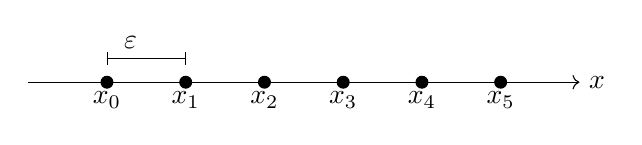
\begin{tikzpicture}
            \draw[->] (-1, 0) -- (6, 0);
            \node[right] at (6, 0) {\(x\)};
            \foreach \x in {0, 1, 2, 3, 4, 5} {
                \draw[fill=black] (\x, 0) circle[radius=0.075cm];
                \node[below] at (\x, 0) {\(x_{\x}\)};
            }
            \draw[|-|] (0, 0.3) -- (1, 0.3);
            \node[above] at (0.3, 0.3) {\(\varepsilon\)};
        \end{tikzpicture}
        \caption{A one dimensional discrete system of \(N = 6\) points, \(x_i\), spaced evenly \(\varepsilon\) apart.}
        \label{fig:one dimensional discrete system}
    \end{figure}
    We can now limit the domain of the wave~function to \(\{x_i\st i=0,\dotsc, 5\}\).
    We define
    \[\psi_i = \sqrt{\varepsilon}\psi(x_i) \in\complex.\]
    We then collect this set of evaluations of \(\psi(x)\) into one object:
    \[
        \ket{\psi} =
        \begin{pmatrix}
            \psi_0\\ \vdots\\ \psi_5
        \end{pmatrix}
    \]
    \(\ket{\psi}\) is a member of a six-dimensional vector space, \(\hilbert\).
    Note that it is wrong to write \(\ket{\psi(x)}\).
    \(\ket{\psi}\) and \(\psi(x)\) are different objects writing \(\ket{\psi(x)}\) is similar to putting a coordinate label on a vector like \(\vv{v}_x\), its just wrong.
    
    \subsubsection{Basis}
    By specifying a vector by its components we assume a basis.
    One such basis is
    \[
        \ket{\xi_0} =
        \begin{pmatrix}
            1\\ 0\\ 0\\ \vdots\\ 0
        \end{pmatrix}
        ,\qquad\ket{\xi_1} =
        \begin{pmatrix}
            0\\ 1\\ 0\\ \vdots\\ 0
        \end{pmatrix}
        ,\dotsc, \ket{\xi_5} =
        \begin{pmatrix}
            0\\ \vdots\\ 0\\ 0\\ 1
        \end{pmatrix}
        .
    \]
    Any vector \(\psi\in\hilbert\) can be written as a linear combination of these basis vectors:
    \[\ket{\psi} = \sum_{k=0}^{5} \psi_k\ket{\xi_k}\]
    where as usual
    \[\psi_k = \braket{\xi_k}{\psi}.\]
    For now we will make some assumptions about extracting physical information from state vectors and wave functions.
    We assume that \(\abs{\psi(x)}^2\) gives the probability density of finding the system at \(x\).
    We also assume that \(\abs{\psi_i}^2 = \varepsilon\abs{\psi(x_i)}^2\) gives the probability of finding the system at \(x_i\).
    Note that the first of these is a probability density and the second is a probability.
    This is because the first is referring to a continuous variable, \(x\), and the second refers to a discrete variable, \(x_i\).
    This is the same as how a probability density function, \(p\), gives a probability, \(p(x)\dd{x}\), here \(\varepsilon\) plays the role of \(\dd{x}\).
    
    With these assumptions we have a physical description of the basis states.
    The vector \(\ket{\xi_i}\) represents a system that is at \(x_i\) with probability 1.
    
    \subsubsection{Scalar Product and Norm}
    We can define a scalar product between \(\ket{\varphi}, \ket{\psi}\in\hilbert\)
    \[\braket{\varphi}{\psi} = \sum_{k=0}^{6} \varphi_k^*\psi_k.\]
    This allows us to induce a norm:
    \[\norm{\psi}^2 = \sum_{k=0}^{6} \abs{\psi_k}^2.\]
    As usual we require state vectors be normalised so
    \[\norm{\psi}^2 = \sum_{k=0}^{6} \abs{\psi_k}^2 = 1.\]
    
    \subsection{Continuous System}
    Moving from this discretised system to a continuous one is as simple as taking the limiting case as \(N \to \infty\) and \(\varepsilon \to 0\).
    After doing this we have that \(\ket{\psi}\in\hilbert_\infty\) where \(\hilbert_\infty\) is an infinite dimensional vector space.
    
    \subsubsection{Basis}
    Define the following basis vectors for our discretised system:
    \[\ket{x_k} = \frac{1}{\sqrt{\varepsilon}}\ket{\xi_k}.\]
    Which gives us \(\ket{\xi_k} = \sqrt{\varepsilon}\ket{x_k}\)
    A vector in the finite dimensional vector space, \(\hilbert\), can be written as
    \[\ket{\psi} = \sum_{k=0}^{N} \psi_k\ket{\xi_k} = \sum_{k=0}^{N} \sqrt{\varepsilon}\psi(x_k)\ket{\xi_k} = \sum_{k=0}^{N} \varepsilon\psi(x_k)\ket{x_k}.\]
    After a limiting process taking \(N\to\infty\) and \(\varepsilon\to 0\) we can write \(\ket{\psi}\in\hilbert_{\infty}\) as
    \[\ket{\psi} = \int\dd{x}\psi(x)\ket{x}\]
    where
    \[\ket{x} = \lim_{\varepsilon\to 0}\frac{1}{\sqrt{\varepsilon}}\ket{\xi_k}.\]
    
    As normal we can find the component, here \(\psi(x)\), with a scalar product with a basis vector:
    \[\psi(x) = \braket{x}{\psi}.\]
    Using this we have
    \[\ket{\psi} = \int\dd{x}\braket{x}{\psi}\ket{x} = \int\dd{x}\ket{x}\braket{x}{\psi}.\]
    We see that \(\ketbra{x}{x}\) is a projection operator and again the completeness relation holds, this time in the form
    \[\int\dd{x}\ketbra{x}{x} = \ident.\]
    
    \subsubsection{Scalar Product and Norm}
    Let \(\ket{\psi}, \ket{\varphi}\in\hilbert\).
    Then their scalar product is
    \[\braket{\varphi}{\psi} = \sum_{k=0}^{N} \varphi_k^*\psi_k = \sum_{k=0}^{N}[\sqrt{\varepsilon}\varphi^*(x_k)][\sqrt{\varepsilon}\psi(x_k)] = \sum_{k=0}^{N}\varepsilon\varphi^*(x_k)\psi(x_k).\]
    After a limiting process taking \(N\to\infty\) and \(\varepsilon\to 0\) we see that for \(\ket{\varphi}, \ket{\psi}\in\hilbert_\infty\) we have
    \[\braket{\varphi}{\psi} = \int\dd{x}\varphi^*(x)\psi(x).\]
    The norm induced by this for \(\ket{\psi}\in\hilbert_\infty\) is given by
    \[\norm{\psi}^2 = \braket{\psi}{\psi} = \int\dd{x}\psi^*(x)\psi(x) = \int\dd{x}\abs{\psi(x)}^2.\]
    For states to be normalisable we require that \(\norm{\psi} < \infty\).
    The space of functions, \(f\colon A\to \complex\), that have this property is called the space of \define{square integrable functions} and is denoted \(\squareIntegrable(A)\).
    For our example of a continuous system we are interested in \(\squareIntegrable(\reals)\).
    If we limit our system to the interval \([a, b]\) where \(a, b\in\reals\) and \(b > a\) then we are interested in the space \(\squareIntegrable([a, b])\).
    
    \subsubsection{Scalar Product of Basis Vectors}
    In the discrete system \(\ket{\xi_k}\) describes a state that is a \(x_k\) with probability 1.
    We want to know what \(\ket{x}\) describes in our continuous case.
    Consider the inner product of two basis states:
    \[\braket{x}{x'} = \lim_{\varepsilon\to 0}\braket{x_k}{x_{k'}} = \lim_{\varepsilon\to 0} \frac{1}{\varepsilon}\braket{\xi_k}{\xi_{k'}}.\]
    Using the orthonormality of \(\{\xi_k\}\) this gives us
    \[
        \braket{x}{x'} = \lim_{\varepsilon\to 0}\frac{1}{\varepsilon}\delta_{kk'} =
        \begin{cases}
            0, & x \ne x',\\
            \infty, &x = x',
        \end{cases}
    \]
    where we have used the fact that if \(x = x'\) then \(\ket{\xi_k} = \ket{\xi_{k'}}\) so \(\delta_{kk'} = \delta_{kk} = 1\) so
    \[\lim_{\varepsilon\to 0} \frac{1}{\varepsilon} = \infty.\]
    On the other hand if \(x \ne x'\) then \(\ket{\xi_k}\ne\ket{\xi_{k'}}\) so \(\delta_{kk'} = 0\).
    Then in the limit we have
    \[\lim_{\varepsilon\to 0}\frac{0}{\varepsilon} = \lim_{\varepsilon\to 0}\frac{\dv{\varepsilon}0}{\dv{\varepsilon}\varepsilon} = \lim_{\varepsilon\to 0}\frac{0}{1} = 0.\]
    We now compute the following integral for reasons that will become clear afterwards:
    \begin{align*}
        \int\dd{x'} f(x')\braket{x}{x'} &= \lim_{\stackrel{N\to \infty}{\varepsilon\to 0}}\sum_{k=0}^{N} \varepsilon f(x_{k'})\braket{x_k}{x_k}\\
        &= \lim_{\stackrel{N\to \infty}{\varepsilon\to 0}}\sum_{k=0}^{N} \varepsilon f(x_{k'})\frac{1}{\varepsilon}\braket{\xi_{k}}{\xi_{k'}}\\
        &= \lim_{N\to\infty}\sum_{k=0}^{N}  f(x_k)\braket{\xi_{k}}{\xi_{k'}}\\
        &= \lim_{N\to\infty} f(x_{k'})\delta_{kk'}\\
        &= \lim_{\varepsilon\to 0}f(x_{k})\\
        &= f(x)
    \end{align*}
    So we see that
    \[\int\dd{x'}f(x')\braket{x}{x'} = f(x)\]
    this, as well as being zero if \(x \ne x'\) defines the \define{Dirac delta distribution}:
    \[
        \delta(x - x') =
        \begin{cases}
            0, & x\ne x',\\
            \infty, & x = x'
        \end{cases}
    \]
    and
    \[\int\dd{x'}f(x')\delta(x - x') = f(x).\]
    So we can identify
    \[\braket{x}{x'} = \delta(x - x').\]
    Using this we get around the fact that \(\{\ket{x}\}\) are not normalisable, that is that \(\braket{x}{x} = \infty\), and we can still extract meaningful information as long as we only have \(\braket{x}{x}\) inside of integrals.
    
    

    \part{Observables}
    \section{Observables}
    In \acrshort{qm} the outcome of a measurement is the outcome of a stochastic variable.
    The theory can only predict the \acrfull{pdf} of the outcome of a given experiment.
    \subsection{Some Statistics}
    A continuous random, or stochastic, variable is one that can take on a different value every time we measure it.
    The values that it can take can be characterised by a \define{\acrfull{pdf}}.
    If \(x\) is a continuous random variable and can take any value in some set \(S\) then the \acrshort{pdf} of \(x\) is a function
    \[p\colon S\to[0, 1]\]
    such that the probability that \(x\) is between \(x\) and \(x + \dd{x}\) is given by \(p(x)\dd{x}\).
    Using this we have that the probability that \(x\) is in the interval \(\mathcal{I} = [a, b]\) is
    \[P(x\in\mathcal{I}) = \int_a^b \dd{x} p(x).\]
    Since probabilities should add up to one we require \(p\) to be properly normalised so that
    \[P(x\in S) = \int_S\dd{x}p(x) = 1.\]
    As a way of characterising a \acrshort{pdf} we define its \define{\(\mathdefine{n}\)th moment} as
    \[\mu_n = \int\dd{x}p(x)x^n.\]
    Clearly if \(p\) is properly normalised then \(\mu_0 = 1\).
    The \define{mean} value of the random variable, \(x\), is
    \[\mu_1 = \expected{x} = \int\dd{x}p(x)x.\]
    The \define{variance} of the variable, \(x\), is
    \[\Var[x] = \mu_2 - (\mu_1)^2 = \expected{x^2} - \expected{x}^2.\]
    
    \subsection{Position Operator}
    The state of the system is described by \(\psi(x) = \braket{x}{\psi}\) where \(\ket{\psi}\in\hilbert\), with \(\hilbert\) being some infinite dimensional vector space that has \(\{\ket{x}\}\) as a basis.
    The \acrshort{pdf} for finding a system in the state \(\ket{\psi}\in\hilbert\) at position \(x\) is
    \[p(x) = \abs{\psi(x)}^2.\]
    The \define{expected value} of \(x\) is
    \[\expected{x} = \int_{-\infty}^{\infty} \dd{x}p(x)x.\]
    We introduce an operator, \(\operator{X}\colon\hilbert\to\hilbert\), defined by
    \[\bra{x}\operator{X}\ket{\psi} = x\braket{x}{\psi},\]
    or, equivalently,
    \[\operator{X}\psi(x) = x\psi(x).\]
    This allows us to write the mean value as
    \begin{align*}
        \expected{x} &= \int\dd{x}\abs{\psi(x)}^2x\\
        &= \int\dd{x}\psi(x)^*x\psi(x)\\
        &= \int\dd{x}\braket{\psi}{x}x\braket{x}{\psi}\\
        &= \int\dd{x}\braket{\psi}{x}\bra{x}\operator{X}\ket{\psi}\\
        &= \bra{\psi}\operator{X}\ket{\psi}\\
        &= \expected{\operator{X}}.
    \end{align*}
    Here we used the completeness relation to get rid of the integral and projection operators.
    Note that \(\expected{\operator{X}}\) is just a short hand for \(\bra{\psi}\operator{X}\ket{\psi}\) when the state \(\psi\) is clear.
    It is not the expected value of the operator \(\operator{X}\) per se but the expected value of \(x\) which is in some way related to the operator \(\operator{X}\).
    
    There is a theorem that states that if we know all the moments of a \acrshort{pdf} then this uniquely determines the \acrshort{pdf}.
    We can find the \(n\)th moment fairly easily:
    \begin{align*}
        \bra{\psi}\operator{X}^n\ket{\psi} &= \int \dd{x} \braket{\psi}{x}\bra{x}\operator{X}^n\ket{\psi}\\
        &= \int \dd{x} \braket{\psi}{x}x^n\braket{x}{\psi}\\
        &= \int \dd{x} \psi(x)^* x^n \psi(x)\\
        &= \int \dd{x} \abs{\psi(x)}^2x^n\\
        &= \int \dd{x} p(x)x^n\\
        &= \mu_n.
    \end{align*}
    So by taking the matrix elements of \(\operator{X}^n\) we can fully describe the \acrshort{pdf}.
    
    Here we have used the following theorem.
    \begin{theorem}{}{op^n ket = eigenvalue^n ket}
        If \(\operator{O}\colon\hilbert\to\hilbert\) is an operator and acts on \(\ket{\psi}\in\hilbert\) as \(\operator{O}\ket{\psi} = z\ket{\psi}\) where \(z\in\complex\) then \(\operator{O}^n\ket{\psi} = z^n\ket{\psi}\).
    \end{theorem}
    \begin{proof}
        We will prove this by induction.
        The basis case of \(n = 0\) holds as by definition \(\operator{O}^0 = \ident\) so
        \[\operator{O}^0\ket{\psi} = \ident\ket{\psi} = \ket{\psi} = 1\ket{\psi} = z^0\ket{\psi}.\]
        Now suppose that this holds for \(n = k\), that is
        \[\operator{O}^k\ket{\psi} = z^k\ket{\psi}.\]
        Then
        \begin{align*}
            \operator{O}^{k+1}\ket{\psi} &= \operator{O}(\operator{O}^k\ket{\psi})\\
            &= \operator{O}(z^k\ket{\psi})\\
            &= z^k(\operator{O}\ket{\psi})\\
            &= z^k(z\ket{\psi})\\
            &= z^{k+1}\ket{\psi}.
        \end{align*}
        So it holds for \(n = k + 1\).
        Thus by induction this holds for all \(n \in\naturals\).
    \end{proof}
    
    \subsection{Generic Observables}
    We define an \define{observable} as a quantity that can be measured in an experiment.
    Here an experiment is a black box that we provide somehow with a prepared state, \(\ket{\psi}\), and after the experiment we are given a value for the observable that we were measuring.
    One important thing that we assume is that the experiment is reproducible, that is that we can prepare the system in the same way and perform the same measurement as many times as needed.
    
    This gives rise to the second postulate of \acrshort{qm}:
    \begin{postulate}{}{}
        In quantum mechanics each observable, \(O\), is associated to a linear operator, \(\operator{O}\colon\hilbert\to\hilbert\).
    \end{postulate}
    The naive approach to find the expected value of an observable, \(O\), given a specific state, \(\ket{\psi}\), might be to try \(\operator{O}\ket{\psi}\).
    However this gives us another vector and we expect real numbers as the results of measurements.
    It turns out that the expected value of \(O\) for a system in the state \(\ket{\psi}\) is given by the matrix elements of \(\operator{O}\):
    \[\expected{O} = \bra{\psi}O\ket{\psi}.\]
    
    \subsubsection{Observing Observables}
    When we say that the value of an observable \(O\) is a stochastic variable is that if we set up the system in state \(\ket{\psi}\) and measure \(O\) and get a result \(O^{(1)}\), and then set up the system in state \(\ket{\psi}\) and measure \(O\) and get a result \(O^{(2)}\), and so on, then we end up with a set of values \(\{O^{(1)}, O^{(2)}, \dotsc, O^{(n)}\}\).
    The important thing is that it is possible that \(O^{(i)}\ne O^{(j)}\), even accounting for experimental error.
    This is very different to classical mechanics where we would expect that a measurement gives the same result every time, up to some level of precision.
    
    The expectation value of \(O\) is then
    \[\expected{O} = \lim_{n\to\infty} \frac{1}{n}\sum_{k=1}^{n} O^{(k)}.\]
    So far we have focused on the value of the observable but with \acrshort{qm} we can predict more than this.
    Given an observable, \(O\), we can predict
    \begin{itemize}
        \item the possible outcomes of a measurement of \(O\),
        \item the probability of obtaining each of these possible outcomes.
    \end{itemize}
    All questions in \acrshort{qm} need to be phrased in terms of possible outcomes and their probabilities, these are the only things that the theory predicts.
    
    \subsection{Eigenvalues and Eigenstates}
    The possible outcomes of measuring an observable, \(O\), are given by the third postulate of \acrshort{qm}:
    \begin{postulate}{}{}
        When measuring an observable, \(O\), the possible outcomes, \(O_k\), are the eigenvalues of the operator, \(\operator{O}\).
    \end{postulate}
    If \(\operator{O}\colon\hilbert\to\hilbert\) and \(\ket{\psi_k}\in\hilbert\) then \(\ket{\psi_k}\) is an \define{eigenvector} or \define{eigenstate} with \define{eigenvalue} \(O_k\) if these are solutions to the following:
    \[\operator{O}\ket{\psi_k} = O_k\ket{\psi_k}.\]
    That is the only result of \(\operator{O}\) when acting on \(\ket{\psi_k}\) is to scale \(\ket{\psi_k}\) by some amount.
    In general in a complex vector space eigenvalues are complex, we will see later that this does not give rise to the correct physics.
    
    If \(O_k\) is an eigenvalue of the operator, \(\operator{O}\), then we say that \(O_k\) is \(g\)-fold degenerate if there are exactly \(g\) linearly independent eigenvectors, \(\ket{u_k^{(n)}}\in\hilbert\) such that
    \[\operator{O}\ket{u_k^{(n)}} = O_k\ket{u_k^{(n)}}\]
    for \(n = 1, \dotsc, g\).
    That is that \(O_k\) is an eigenvalue for \(g\) fundamentally different eigenvectors (as opposed to scaled versions of the same eigenvector).
    
    Any linear combination of the form
    \[\sum_{n=1}^{g}c_n\ket{u_k^{(n)}}\]
    where \(c_k\in\complex\) is also an eigenstate of \(\operator{O}\), this is fairly easy to show using the linearity of \(\operator{O}\):
    \begin{align*}
        \operator{O}\sum_{n=1}^{g}c_n\ket{u_k^{(n)}} &= \sum_{n=1}^{g}c_n\operator{O}\ket{u_k^{(n)}}\\
        &= \sum_{n=1}^{g}c_nO_k\ket{u_k^{(n)}}\\
        &= O_k\sum_{n=1}^{g}c_n\ket{u_k^{(n)}}.
    \end{align*}
    In fact any set of eigenvectors with degenerate eigenvalues forms a \(g\)-dimensional vector subspace of \(\hilbert\).
    
    One logical question that we may ask now is what do the eigenstates represent?
    We can try to measure the expected value of \(O\) in a system that is the state \(\ket{\psi_k}\) which is an eigenstate of \(\operator{O}\) with eigenvalue \(O_k\).
    We get
    \begin{align*}
        \expected{O} &= \bra{\psi_k}\operator{O}\ket{\psi_k}\\
        &= \bra{\psi_k}O_k\ket{\psi_k}\\
        &= O_k\braket{\psi_k}{\psi_k}\\
        &= O_k.
    \end{align*}
    So the expected value of \(O\) measured on its eigenstate, \(\ket{\psi_k}\), is \(O_k\).
    We can also compute the variance:
    \begin{align*}
        \Var_{\psi_k}[O] &= \expected{O^2} - \expected{O}^2\\
        &= \bra{\psi_k}\operator{O}^2\ket{\psi_k} - [\bra{\psi_k}\operator{O}\ket{\psi_k}]^2\\
        &= \bra{\psi_k}O_k^2\ket{\psi_k} - [\bra{\psi_k}O_k\ket{\psi_k}]^2\\
        &= O_k^2\braket{\psi_k}{\psi_k} - [O_k\braket{\psi_k}{\psi_k}]^2\\
        &= O_k^2 - O_k^2\\
        &= 0.
    \end{align*}
    where we have used the result of theorem~\ref{thm:op^n ket = eigenvalue^n ket}, which states \(\operator{O}^2\ket{\psi_k} = O_k^2\ket{\psi_k}\) so
    \[\bra{\psi_k}\operator{O}^2\ket{\psi_k} = \bra{\psi_k}O_k^2\ket{\psi_k} = O_k^2\braket{\psi_k}{\psi_k}.\]
    The important thing is that the expected value is \(O_k\) and the variance is zero.
    This means that there is no spread in the values measured and so \(O^{(i)} = O_k\) for all \(i\).
    This means that in the state \(\ket{\psi_k}\) when we measure \(O\) we get \(O_k\) with probability 1.
    
    \subsection{Hermitian Operators}
    \subsubsection{Hermitian Conjugate}
    Let \(\operator{O}\colon\hilbert\to\hilbert\).
    Then we define the \define{hermitian conjugate} of \(\operator{O}\), denoted \(\operator{O}\hermit\), to be another operator, \(\operator{O}\hermit\colon\hilbert\to\hilbert\), defined such that for all \(\ket{\varphi}, \ket{\psi}\in\hilbert\)
    \[\bra{\varphi}\operator{O}\hermit\ket{\psi} = [\bra{\psi}\operator{O}\ket{\varphi}]^*.\]
    Compare this to the usual linear algebra definition:
    \[O_{ij}\hermit = O_{ji}^*.\]
    We see that since \(\bra{\varphi}\operator{O}\hermit\ket{\psi}\) gives the matrix elements of \(\operator{O}\hermit\) these two definitions are equivalent.
    
    \begin{example}\label{exa:hermitian conjugate of the derivative}
        Consider the operator \(\operator{O} = \dv{x}\) defined by
        \begin{align*}
            \bra{x}\operator{O}\ket{\psi} &= \bra{x}\dv{x}\ket{\psi}\\
            &= \dv{x}\braket{x}{\psi}\\
            &= \dv{x}\psi(x).
        \end{align*}
        Compute \(\operator{O}\hermit\).
        \begin{align*}
            \bra{\varphi}\operator{O}\hermit\ket{\psi} &= [\bra{\psi}\operator{O}\ket{\varphi}]^*
            \shortintertext{inserting completeness gives}
            &= \left[ \int_{-\infty}^{\infty} \dd{x} \braket{\psi}{x}\bra{x}\operator{O}\ket{\varphi} \right]^*\\
            &= \left[ \int_{-\infty}^{\infty} \dd{x} \psi(x)^*\dv{x}\varphi(x) \right]^*.\stepcounter{equation}\tag{\theequation}\label{eqn:int psi d/dx phi}
        \end{align*}
        We can now integrate by parts:
        \[
            \begin{array}{ll}
                u = \psi(x)^*, & v = \varphi(x),\\
                u' = \dv{x}\psi(x)^*, & v' = \dv{x}\varphi(x).
            \end{array}
        \]
        \begin{align*}
            \bra{\varphi}\operator{O}\hermit\ket{\psi} &= \left[ [\psi(x)^*\varphi(x)]_{-\infty}^{\infty} - \int_{-\infty}^{\infty} \dd{x} \varphi(x)\dv{x}\psi(x)^* \right]^*
            \shortintertext{this first term is zero as \(\psi\) and \(\varphi\) are wave functions so are square integrable so they vanish at infinity leaving us with}
            &= \left[ -\int_{-\infty}^{\infty} \dd{x} \varphi(x)\dv{x}\psi(x)^* \right]^*\\
            &= -\int_{-\infty}^{\infty} \dd{x} \varphi(x)^*\dv{x}\psi(x)\\
            &= -\int_{-\infty}^{\infty} \dd{x} \braket{\varphi}{x}\bra{x}\operator{O}\ket{\psi}\\
            &= -\bra{\varphi}\operator{O}\ket{\psi}.
        \end{align*}
        So we can identify
        \[\left(\dv{x}\right)\hermit = -\dv{x}.\]
    \end{example}
    
    \subsubsection{Hermitian Operator}
    An operator, \(\operator{O}\colon\hilbert\to\hilbert\), is \define{hermitian} if \(\operator{O}\hermit = \operator{O}\).
    We saw in example~\ref{exa:hermitian conjugate of the derivative} that \(\dv{x}\) is \emph{not} hermitian as \(\operator{O}\hermit = -\operator{O}\), this property is actually called being \define{anti-hermitian}.
    \begin{example}\label{exa:momentum operator hermitian}
        Show that \(\operator{O} = -i\hbar\dv{x}\) is hermitian.
        This operator will be important later.
        \begin{align*}
            \bra{\varphi}\operator{O}\hermit\ket{\psi} &= [\bra{\psi}\operator{O}\ket{\varphi}]^*\\
            &= \left[ \int_{-\infty}^{\infty} \dd{x} \braket{\psi}{x}\bra{x}\operator{O}\ket{\varphi} \right]^*\\
            &= \left[ \int_{-\infty}^{\infty} \dd{x} \psi(x)\left(-i\hbar\dv{x}\right) \ket{\varphi}\right]^*\\
            &= \left[ -i\hbar\int_{-\infty}^{\infty} \dd{x} \psi(x)\dv{x} \varphi(x)\right]^*\\
            &= i\hbar \int_{-\infty}^{\infty} \dd{x} \psi(x)^*\dv{x}\varphi(x)\\
            \shortintertext{see equation~\ref{eqn:int psi d/dx phi} for how to do this integral}
            &= -i\hbar \int_{-\infty}^{\infty} \dd{x} \varphi(x)^*\dv{x}\psi(x)\\
            &= \int_{-\infty}^{\infty} \dd{x} \varphi(x)^*\left(-i\hbar\dv{x}\right) \psi(x)\\
            &= \int_{-\infty}^{\infty} \dd{x} \braket{\varphi}{x}\bra{x}\operator{O}\ket{\psi}\\
            &= \bra{\varphi}\operator{O}\ket{\psi}.
        \end{align*}
        So we can identify that
        \[\left(-i\hbar\dv{x}\right)\hermit = -i\hbar\dv{x}\]
        so this is a hermitian operator.
    \end{example}
    \subsubsection{Properties of Hermitian Operators}
    The following important properties of hermitian operators make incredibly important to \acrshort{qm}:
    \begin{enumerate}
        \item Hermitian operators have real eigenvalues.
        That is if \(\operator{O}\colon\hilbert\to\hilbert\) and
        \[\operator{O}\ket{\psi_k} = O_k\ket{\psi_k}\]
        then
        \[\operator{O} = \operator{O}\hermit \implies O_k\in\reals.\]
        
        \item The eigenstates of a hermitian operator that belong to different eigenvalues are orthogonal.
        That is if \(\operator{O}\colon\hilbert\to\hilbert\),
        \[\operator{O}\ket{\psi_k} = O_k\ket{\psi_k}, \qquad\text{and}\qquad \operator{O}\ket{\psi_l} = O_l\ket{\psi_l}\]
        where \(O_k \ne O_l\) then
        \[\braket{\psi_k}{\psi_l} = 0.\]
        
        \item If \(\operator{O}\colon\hilbert\to\hilbert\) then there exists an orthogonal basis of \(\hilbert\) made of eigenvectors of \(\operator{O}\).
        In other words \(\ket{\psi}\in\hilbert\) can be written as
        \[\ket{\psi} = \sum_k c_k\ket{\psi_k}\]
        where \(c_k\in\complex\) are given by
        \[c_k = \braket{\psi_k}{\psi}.\]
    \end{enumerate}
    We can prove these fairly easily:
    \begin{theorem}{}{}
        Hermitian operators have real eigenvalues.
    \end{theorem}
    \begin{proof}
        Suppose \(\operator{O}\) is a hermitian operator on \(\hilbert\).
        Let \(\ket{\psi_k}\) be a normalised eigenvector of \(\operator{O}\) with eigenvalue \(O_k\).
        Then
        \[\operator{O}\ket{\psi_k} = O_k\ket{\psi_k}.\]
        Taking an inner product with \(\bra{\psi_k}\) we get
        \begin{equation}\label{eqn:psi_k O psi_k = O_k}
            \bra{\psi_k}\operator{O}\ket{\psi_k} = \bra{\psi_k}O_k\ket{\psi_k} = O_k\braket{\psi_k}{\psi_k} = O_k
        \end{equation}
        where we have used the fact that \(\ket{\psi_k}\) is normalised so \(\braket{\psi_k}{\psi_k} = 1\).
        Taking the complex conjugate of this equation gives us
        \[[\bra{\psi_k}\operator{O}\ket{\psi_k}]^* = O_k^*.\]
        Using the definition of the hermitian conjugate the left hand side is equivalent to
        \[\bra{\psi_k}\operator{O}\hermit\ket{\psi_k}.\]
        Since \(\operator{O}\) is hermitian this in turn is equivalent to
        \[\bra{\psi_k}\operator{O}\ket{\psi_k},\]
        which, as we saw in equation~\ref{eqn:psi_k O psi_k = O_k}, is just \(O_k\).
        This means that we have
        \[O_k = O_k^*\]
        which can only be true if \(O_k\in\reals\).
    \end{proof}
    \begin{theorem}{}{}
        The eigenfunctions of a hermitian operator which belong to different eigenvalues are orthogonal.
    \end{theorem}
    \begin{proof}
        Let \(\operator{O}\) be an operator on \(\hilbert\).
        Suppose that
        \[\operator{O}\ket{\psi_1} = O_1\ket{\psi_1}, \qquad\text{and}\qquad \operator{O}\ket{\psi_2} = O_2\ket{\psi_2}\]
        where \(O_1 \ne O_2\).
        Taking the inner product of the first of these equations with \(\bra{\psi_2}\) we have
        \begin{equation}\label{eqn:psi_2 O psi_1 = O_1 psi_2 psi_1}
            \bra{\psi_2}\operator{O}\ket{\psi_1} = O_1\braket{\psi_2}{\psi_1}.
        \end{equation}
        Instead taking the inner product of the second equation with \(\bra{\psi_1}\) we have
        \[\bra{\psi_1}\operator{O}\ket{\psi_2} = O_2\braket{\psi_1}{\psi_2}.\]
        Taking the complex conjugate, using the definition of the hermitian conjugate, and then using the fact that \(\operator{O}\hermit = \operator{O}\) the left hand side of the above equation gives us
        \[[\bra{\psi_1}\operator{O}\ket{\psi_2}]^* = \bra{\psi_2}\operator{O}\hermit\ket{\psi_1} = \bra{\psi_2}\operator{O}\ket{\psi_1}.\]
        The right hand side gives
        \[O_2^*\braket{\psi_1}{\psi_2} = O_2\braket{\psi_1}{\psi_2},\]
        where we have used the fact that \(\operator{O}\) is hermitian so its eigenvalues are real and therefore \(O_2^* = O_2\).
        Comparing this with equation~\ref{eqn:psi_2 O psi_1 = O_1 psi_2 psi_1} we see that
        \[O_2\braket{\psi_2}{\psi_1} = O_1\braket{\psi_2}{\psi_1}\]
        which gives us
        \[(O_2 - O_1)\braket{\psi_2}{\psi_1} = 0.\]
        Given that \(\complex\) is a field and so has no zero divisors either \(O_2 - O_1 = 0\) or \(\braket{\psi_2}{\psi_1} = 0\).
        By our assumption \(O_2 - O_1\ne 0\) so we must have \(\braket{\psi_2}{\psi_1} = 0\).
        This means that \(\ket{\psi_1}\) and \(\ket{\psi_2}\) are orthogonal.
    \end{proof}
    
    The reason that the first of these properties, that the eigenvalues are real, is important is that we expect real results from an experiment and therefore it only makes sense to have the eigenvalues of an observable be real.
    The other two properties become useful when doing theory as working in the basis given by the eigenvectors, called the eigenbasis, can simplify a lot of equations.
    The process of moving into this eigenbasis is called spectral decomposition.
    
    \subsubsection{Spectral Decomposition}
    \begin{postulate}{}{}
        An observable, \(O\), has an associated hermitian linear operator, \(\operator{O}\colon\hilbert\to\hilbert\), which has a nondegenerate eigenvalue \(O_k\) and associated eigenvector \(\ket{\psi_k}\).
        Given a normalised state, \(\ket{\psi}\in\hilbert\), the probability of measuring \(O\) to be \(O_k\) is
        \[P_k = \abs{c_k}^2 = \abs{\braket{\psi_k}{\psi}}^2\]
        where \(c_k\in\complex\) are the coordinates of \(\ket{\psi}\) in the basis made of the eigenvectors of \(\operator{O}\):
        \[\ket{\psi} = \sum_{k}c_k\ket{\psi_k}.\]
        In the case that \(O_k\) is \(g\)-fold degenerate and has the vectors \(\{\ket{u_k^{(n)}}\}\) as its eigenvectors then the probability of measuring \(O\) to be \(O_k\) is instead the sum of the contributions from the whole subspace spanned by \(\{\ket{u_k^{(n)}}\}\):
        \[P_k = \sum_{n=1}^{g} \abs{\braket{u_k^{(n)}}{\psi}}^2.\]
    \end{postulate}
    This postulate is the reason that we require states be normalised because this means that
    \[\sum_k P_k = \sum_k\sum_{n=1}^{g_k}\abs{\braket{u_k^{(n)}}{\psi}}^2 = 1,\]
    where \(g_k\) is the degeneracy of the eigenvalue \(O_k\).
    In the case of non-degenerate eigenvalues the second sum has only one term and we recover the more familiar requirement that
    \[\sum_k \abs{\braket{\psi_k}{\psi}}^2 = 1.\]
    
    
    \section{Collapse of the State Vector}
    Suppose we have a state \(\ket{\psi}\) and we measure the observable \(O\) and get a value of \(O_k\) which has the associated eigenvector \(\ket{\psi_k}\).
    Immediately after performing this measurement we know that the value of \(O\) is \(O_k\) with probability 1.
    This must mean that the system is in state \(\ket{\psi_k}\).
    The act of measuring changes the state of the system.
    This is true for all measurements we could make.
    \begin{postulate}{}{}
        Immediately after a measurement that gives the result \(O_k\), where \(O_k\) is a non-degenerate eigenvalue of \(\operator{O}\), the state of the system is \(\ket{\psi_k}\), which is the eigenvector associated with \(O_k\).
        The state vector has been projected onto the eigenstate by the process of performing the measurement.
    \end{postulate}
    Mathematically what this looks like is we start with a state, \(\ket{\psi}\), and perform some sort of measurement.
    The outcome of the measurement is \(O_k\) with probability \(\abs{\braket{\psi_k}{\psi}}^2\).
    After the experiment the state is
    \[\frac{1}{\sqrt{\bra{\psi}\operator{\proj}_k\ket{\psi}}}\operator{\proj}_k\ket{\psi}.\]
    Here \(\operator{\proj}_k = \ketbra{\psi_k}{\psi_k}\) is the projection operator onto the eigenspace of \(\ket{\psi_k}\).
    
    If instead \(O_k\) has degeneracy \(g_k\) then
    \[\operator{\proj}_k = \sum_{n=1}^{g_k} \ketbra{u_k^{n}}{u_k^{(n)}}\]
    where \(\ket{u_k^{(n)}}\) are the eigenvectors with eigenvalue \(O_k\) for \(n = 1, \dotsc, g_k\).
    The state after measurement is then
    \[\frac{1}{\sqrt{\sum_{n=1}^{g_k}\abs{c_k^{(n)}}^2}} \sum_{n=1}^{g_k}c_k^{(n)} \ket{u_k^{(n)}}.\]
    
    \subsection{Compatible Observables}
    Suppose \(A\) and \(B\) are observables.
    If we take three measurements, first measuring \(A\), then \(B\), then \(A\) again, \(A\) and \(B\) are said to be \define{compatible} if and only if the result of the third measurement is equal to the result of the first measurement with probability one.
    That is measuring \(B\) doesn't change the outcome of measuring \(A\).
    
    Suppose that \(A\) and \(B\) have associated operators \(\operator{A}\) and \(\operator{B}\) respectively, which have no degenerate eigenvalues.
    Suppose also that
    \[\operator{A}\ket{u_i} = A_i\ket{u_i}, \qquad\text{and}\qquad \operator{B}\ket{v_i} = B_i\ket{v_i}.\]
    After we measure \(A\) if we get a value of \(A_j\) then the state of the system is \(\ket{u_j}\).
    Next we measure \(B\) and we get \(B_k\) meaning that the system is in the state \(\ket{v_k}\).
    The only way that we can guarantee another measurement of \(A\) will yield the same value as the first is if \(\ket{v_k} = \ket{u_j}\).
    For this to hold for all possible values of the measurement we must have that \(\ket{v_k} = \ket{v_j}\) for all possible values of \((i, j)\).
    If there is no degeneracy then we have a one to one correspondence between eigenvectors of \(\operator{A}\) and eigenvectors of \(\operator{B}\).
    We say that \(\operator{A}\) and \(\operator{B}\) have a common eigenbasis.
    
    The conditions under which \(A\) and \(B\) are compatible are summarised in the compatibility theorem:
    \begin{theorem}{The Compatibility Theorem}{}
        Given two observables, \(A\) and \(B\), with associated operators \(\operator{A}\) and \(\operator{B}\), then the following are equivalent:
        \begin{enumerate}
            \item \(A\) and \(B\) are compatible observables,
            \item \(\operator{A}\) and \(\operator{B}\) have a common eigenbasis,
            \item The operators \(\operator{A}\) and \(\operator{B}\) commute: \([\operator{A}, \operator{B}] = 0\).
        \end{enumerate}
    \end{theorem}
    Due to the third condition compatible observables are sometimes called \define{commuting observables}.
    
    \subsection{Complete Sets of Compatible observables}
    Consider an observable \(A\) with associated operator \(\operator{A}\).
    Let the eigenbasis of \(\operator{A}\) be \(\{u_i\}\).
    In the case of no degeneracy we have
    \[\operator{A}\ket{u_k} = a_k\ket{u_k}.\]
    We can identify the eigenvector \(\ket{u_k}\) by its eigenvalue, which we do by writing it \(\ket{a_k}\).
    \(A\) is then trivially a \gls{csco} by itself.
    
    In the case where there is degeneracy we can introduce another observable, \(B\), which is compatible with \(A\).
    It is possible to find a common eigenbasis of \(\operator{A}\) and \(\operator{B}\).
    Call this eigenbasis \(\{\ket{v_k^{(n)}}\}\) where \(n=1,\dotsc, g_k\).
    Suppose that
    \[\operator{A}\ket{v_k^{(n)}} = a_i\ket{v_k^{(n)}}, \qquad\text{and}\qquad \operator{B}\ket{v_k^{(n)}} = b_j\ket{v_k^{(n)}}.\]
    If \((a_i, b_j)\) uniquely identifies this eigenstate then \(A\) and \(B\) are a \gls{csco}.
    We then write \(\ket{v_{k}^{(n)}} = \ket{a_i, b_j}\).
    
    If \((a_i, b_j)\) does not uniquely identify \(\ket{v_k^{(n)}}\) then we simply keep introducing observables that are compatible with all previously introduced observables until we have a tuple of eigenvalues that does uniquely identify each eigenvector.
    
    That is \(\{A, B, C, \dotsc\}\) is a \define{\acrfull{csco}} if and only if:
    \begin{itemize}
        \item All observables commute in pairs,
        \item Specifying all the eigenvalues of the operators identifies a unique eigenvector in the common eigenbasis.
    \end{itemize}

    Given a \gls{csco}, for example, \(\{A, B, C\}\), we can expand a state in the common eigenbasis as
    \[\ket{\psi} = \sum_{n, p, q}c_{npq}\ket{a_n,b_p,c_q}.\]
    The probability of measuring \(a_n\), \(b_p\), and \(c_q\) simultaneously is then \(\abs{c_{npq}}^2\).
    
    \section{Continuous Spectra}
    Up to now we have only considered eigenvalues and eigenvectors that can be identified by a discrete variable, \(k\).
    We can also have eigenvalues that are represented by a continuous variable, \(f\).
    For example
    \[\operator{f}\ket{f} = f\ket{f}\]
    where we follow the convention of identifying an eigenvector by the associated eigenvalue.
    Assuming that \(\operator{f}\) is hermitian then \(f\in\reals\).
    The completeness relation for a continuous basis set is
    \[\int\dd{f}\ketbra{f}{f} = \ident.\]
    We can expand a generic state, \(\ket{\psi}\), in this basis:
    \[\ket{\psi} = \int\dd{f} c(f)\ket{f}.\]
    Here \(c(f)\) plays the role of the coordinates of \(\ket{\psi}\) in the same way that \(c_k\) did in the discrete case.
    The method for computing \(c(f)\) is the same as in the discrete case:
    \begin{align*}
        c(f) &= \braket{f}{\psi}\\
        &= \int\dd{x} \braket{f}{x}\braket{x}{\psi}\\
        &= \int\dd{x} f^*(x)\psi(x).
    \end{align*}
    Since we now have a continuous variable the probability of any one particular value has to be zero.
    However \(\abs{c(f)}^2\) does give the probability density such that
    \[P(f\in[f_-, f_+]) = \int_{f_-}^{f_+} \dd{f} \abs{c(f)}^2.\]
    To be properly normalised we demand that
    \[\int_{-\infty}^{\infty} \dd{f}\abs{c(f)}^2 = 1.\]
    
    Perhaps the most common continuous observable to consider is the position.
    The operator for position is \(\operator{X}\) and its action on \(\ket{\psi}\) is
    \[\operator{X}\ket{\psi} = x\ket{\psi}.\]
    Note that this is \emph{not} an eigenvalue equation, \(x\) is a variable not a constant and this holds for all \(\ket{\psi}\).
    This is simply a statement that the action of \(\operator{X}\) is to multiply the state by \(x\).
    The effect that this has on the wave function is as we would expect:
    \begin{align*}
        \operator{X}\ket{\psi} &= \operator{X}\left[\int\dd{x} \psi(x)\ket{x}\right]\\
        &= \int\dd{x} \psi(x)\operator{X}\ket{x}\\
        &= \int\dd{x} \psi(x)x\ket{x}\\
        &= \int\dd{x} \varphi(x)\ket{x}\\
        &= \ket{\varphi}
    \end{align*}
    where \(\ket{\varphi}\) is defined to be such that \(\braket{x}{\varphi} = \varphi(x) = x\psi(x)\).
    Being slightly lazy with notation we will sometimes write things like
    \[\operator{X}\psi(x) = x\psi(x)\]
    which is not, strictly speaking, defined as operators can only act on elements of \(\hilbert\), not on the coordinates of these vectors.
    However the meaning should be clear enough that it doesn't matter.
    
    \subsection{Orthonormality}
    Suppose that \(f\) and \(f'\) distinct eigenvalues of \(\operator{f}\).
    Then by definition
    \[\operator{f}\ket{f} = f\ket{f},\qquad\text{and}\qquad \operator{f}\ket{f'} = f'\ket{f'}.\]
    We can compute matrix elements of \(\operator{f}\):
    \[\bra{f'}\operator{f}\ket{f} = f\braket{f'}{f},\]
    or using the hermitian property of \(\operator{f}\):
    \begin{align*}
        \bra{f'}\operator{f}\ket{f} &= (\bra{f}\operator{f}\hermit\ket{f'})^*\\
        &= (\bra{f}\operator{f}\ket{f'})^*\\
        &= (f'\braket{f}{f'})^*\\
        &= {f'}^*(\braket{f}{f'})^*\\
        &= f'\braket{f'}{f}.
    \end{align*}
    Hence
    \[(f - f')\braket{f'}{f} = 0.\]
    Assuming that \(f \ne f'\) then \(f - f' \ne 0\) so \(\braket{f'}{f} = 0\).
    
    Consider the state \(\ket{\psi}\) expanded in this basis:
    \[\ket{\psi} = \int\dd{f} c(f)\ket{f}.\]
    We can compute \(\norm{\psi}\):
    \begin{align*}
        \norm{\psi}^2 &= \braket{\psi}{\psi}\\
        &= \int\dd{f'}f^*(f')\bra{f'}\int\dd{f}c(f)\ket{f}\\
        &= \int\dd{f'}\dd{f}c^*(f)c(f)\braket{f'}{f}\\
        &= \int\dd{f}c^*(f)c(f)\braket{f}{f}\\
        &= \int\dd{f}\abs{c(f)}^2\braket{f}{f}
    \end{align*}
    Here we have used that \(\braket{f'}{f}\) is zero apart from when \(f = f'\) to replace \(f'\) with \(f\) while removing one of the integrals.
    We also require that \(\norm{\psi} = 1\) and we already have that
    \[\int\abs{c(f)}^2 = 1\]
    so we must have
    \[\int\dd{f}\braket{f}{f} = 1.\]
    The properties that we have described so far for \(\braket{f'}{f}\) are exactly the definition of the Dirac delta function:
    \[\braket{f'}{f} = \delta(f - f').\]
    
    \begin{example}
        Consider a system on a line.
        The position operator, \(\operator{X}\), is defined as
        \[\operator{X}\ket{x} = x\ket{x}.\]
        A generic state is
        \[\ket{\psi} = \int\dd{x}\psi(x)\ket{x}\]
        where
        \[\psi(x) = \braket{x}{\psi}.\]
        By definition
        \[\braket{x}{x'} = \delta(x - x').\]
        Thus
        \begin{align*}
            \braket{\psi}{\psi} &= \int\dd{x}\dd{x'}\psi^*(x)\psi(x')\braket{x}{x'}\\
            &= \int\dd{x}\dd{x'}\psi^*(x)\psi(x')\delta(x - x')\\
            &= \int\dd{x}\psi^*(x)\psi(x)\\
            &= \int\dd{x}\abs{\psi(x)}^2.
        \end{align*}
        Consider now the state that has a wave function given by
        \[\psi(x) = c\exp\left[\frac{i}{\hbar}p_0x - \frac{(x - x_0)^2}{2\xi^2}\right]\]
        where \(x_0\), \(p_0\), and \(\xi\) are constants and \(c\in\reals\) is a normalisation factor.
        \begin{align*}
            \braket{\psi}{\psi} &= \int_{-\infty}^{\infty} \abs{\psi(x)}^2\\
            &= \int_{-\infty}^{\infty} c^2\exp\left[-\frac{(x - x_0)^2}{2\xi^2}\right]\\
            &= c^2\xi\sqrt{\pi}.
        \end{align*}
        Requiring a normalised state we then have
        \[c = \frac{1}{\pi^{1/4}\sqrt{\xi}}.\]
        The expected position is given by
        \begin{align*}
            \expected{x} &= \int\dd{x} x\abs{\psi(x)}^2\\
            &= \frac{1}{\xi\sqrt{\pi}}\int\dd{x} x\exp\left[-\frac{(x - x_0)^2}{2\xi^2}\right]\\
            &= x_0.
        \end{align*}
        Similarly it can be shown that
        \[\expected{\Delta x^2} = \expected{(x - x_0)^2} = \xi^2.\]
        This can be shown by computing the integrals or recognising the integrands as Gaussians and hence we are simply computing the moments of this distribution.
    \end{example}
    \subsection{Momentum Operator}
    The momentum operator, \(\operator{P}\colon\hilbert\to\hilbert\), is defined by
    \[\bra{x}\operator{P}\ket{\psi} = \operator{P}\psi(x) = -i\hbar\dv{x}\psi(x).\]
    We saw in example~\ref{exa:momentum operator hermitian} that this is a hermitian operator.
    One justification for calling this a momentum operator comes from a plane wave with momentum \(p\):
    \[\psi_p(x) = \exp\left[\frac{ipx}{\hbar}\right].\]
    When we act on this with the momentum operator we get
    \begin{align*}
        \operator{P}\psi_p(x) &= -i\hbar\dv{x}\exp\left[\frac{ipx}{\hbar}\right]\\
        &= -i\hbar\frac{ip}{\hbar}\exp\left[\frac{ipx}{\hbar}\right]\\
        &= p\psi_p(x)
    \end{align*}
    So, at least in this case, the momentum is an eigenvalue of \(\operator{P}\).
    
    Momentum is a conserved variable.
    By Noether's every conserved variable has a related transformation.
    The transformation related to momentum is translations.
    We can describe a small translation about the coordinate \(x\) by an amount \(a\) as
    \[\psi(x + a) = \psi(x) + a\dv{x}\psi(x) + \order{a^2}.\]
    However \(\inlinedv{}{x}\) is an anti-hermitian operator.
    Fortunately there is an easy fix for this, if \(A\) is anti-hermitian then \(iA\) is hermitian.
    This means we can write
    \[\psi(x + a) = \psi(x) + \frac{i}{\hbar}\left(-i\hbar\dv{x}\right)\psi(x) + \order{a^2}.\]
    The factor of \(\hbar\) is convention and ensures that we have the correct units.
    In this way the momentum operator is the generator of translations.
    
    \subsection{The Canonical Commutation Relation}
    Consider the two operators that we have met so far that are related to actual observables, the position, \(\operator{X}\), and momentum, \(\operator{P}\).
    The commutator of these two operators is fairly easy to compute:
    \begin{align*}
        \operator{X}\operator{P}\psi(x) &= \operator{X}\left[-i\hbar\dv{x}\psi(x)\right]\\
        &= -i\hbar x\dv{x}\psi(x)\\
        \operator{P}\operator{X}\psi &= \operator{P}x\psi(x)\\
        &= -i\hbar\dv{x}[x\psi(x)]\\
        &= -i\hbar x\dv{x}\psi(x) - i\hbar\psi(x)\\
        [\operator{X}, \operator{P}]\psi &= \operator{X}\operator{P} - \operator{P}\operator{X}\\
        &= -i\hbar x\dv{x}\psi(x) + i\hbar x\dv{x}\psi(x) + i\hbar\psi(x)\\
        &= i\hbar\psi(x)
    \end{align*}
    This holds for all \(\psi\) therefore we conclude that
    \begin{empheq}[box=\tcbhighmath]{equation*}
        [\operator{X}, \operator{P}] = i\hbar.
    \end{empheq}
    This is called the \define{canonical commutation relation}.
    From this we can derive the \define{\gls{hup}}:
    \begin{empheq}[box=\tcbhighmath]{equation*}
        \Delta x\Delta p \ge \frac{\hbar}{2}.
    \end{empheq}

    \part{Dynamics}
    \section{Dynamics}
    \subsection{Dynamics in Classical Mechanics}
    In classical mechanics the dynamics of a system can be entirely determined from Newton's second law:
    \[\vv{F} = m\vv{a} = m\dv[2]{\vv{r}}{t}.\]
    The force term encodes information about the external forces applied to the system, the mass is a characteristic of the system and the acceleration provides a time dependence.
    Solving this differential equation can give us the equations of motion.
    From these we can predict the future of the system but also the past.
    
    \subsection{Dynamics in Quantum Mechanics}
    \begin{postulate}
        The dynamics of a system described by the state \(\ket{\Psi(t)}\), at time \(t\), is determined by the \define{Schr\"odinger equation}:
        \begin{empheq}[box=\equationBox]{equation*}
            i\hbar\dv{t}\ket{\Psi(t)} = \operator{H}\ket{\Psi(t)}.
        \end{empheq}
        Where \(\operator{H}\) is the \define{Hamiltonian}, a hermitian operator corresponding to the energy of the system.
    \end{postulate}
    The state vectors, \(\ket{\Psi(t)}\), now include an explicit time dependence.
    
    The Hamiltonian, for a single particle in one dimension, is given in an analogous way to classical mechanics by
    \[\operator{H} = \operator{T} + \operator{V}.\]
    Here \(\operator{T}\) is the operator associated with the kinetic energy and \(\operator{V}\) is the operator associated with the potential energy.
    In general it is often possible to take a classical formula and change \(x\) to \(\operator{X}\), and \(p\) to \(\operator{P}\) and have it still be valid, although we do have to be careful about whether operators commute which we don't have to consider with classical mechanics.
    Fortunately this is valid for this case and we have
    \begin{align*}
        T = \frac{p^2}{2m} &\rightarrow \operator{T} = \frac{\operator{P}^2}{2m},\\
        V = V(x) &\rightarrow \operator{V} = V(\operator{X}).
    \end{align*}
    Here the function \(V\) on the left, which acts on real numbers, and the function \(V\) on the right, which acts on operators, are technically different as their domains are different but they have the same form.
    For example in a harmonic potential,
    \[V(x) = \frac{1}{2}kx^2\]
    and the operator equivalent is
    \[V(\operator{X}) = \frac{1}{2}k\operator{X}^2.\]
    Consider a state \(\ket{\Psi(t)}\), after a small amount of time, \(\varepsilon\), this becomes
    \begin{align*}
        \ket{\Psi(t + \varepsilon)} &= \ket{\Psi(t)} + \varepsilon\dv{t}\ket{\Psi(t)}\\
        &= \ket{\Psi(t)} - \frac{i\varepsilon}{\hbar}\operator{H}\ket{\Psi(t)}
    \end{align*}
    In this way we can view the change in time as the result of the action of \(\operator{H}\).
    
    \subsection{Time Evolution of a Wave Function}
    The wave function related to the state \(\ket{\Psi(t)}\) is, as normal, found by the inner product with the position eigenbasis vectors:
    \[\Psi(x, t) = \braket{x}{\Psi(t)}.\]
    If we take the inner product of the left hand side of the Schr\"odinger equation with one of these basis vectors we get
    \[\bra{x}i\hbar\dv{t}\ket{\Psi(t)} = i\hbar\dv{t}\braket{x}{\Psi(t)} = i\hbar\pdv{t}\Psi(x, t).\]
    Here we have used the fact that \(\bra{x}\) is independent of time so commutes with a time derivative.
    Taking the inner product with the right hand side we have
    \[\bra{x}\operator{H}\ket{\Psi(t)} = \operator{H}\braket{x}{\Psi(t)} = \operator{H}\Psi(x, t).\]
    
    In the case that \(\operator{H} = \operator{T} + \operator{V}\),
    \[\operator{T} = \frac{\operator{P}^2}{2m},\qquad\text{and}\qquad \operator{V} = V(\operator{X})\]
    the Schr\"odinger equation becomes
    \[\operator{H}\Psi(x, t) = \left[\frac{\operator{P^2}}{2m} + V(\operator{X})\right]\Psi(x, t) = i\hbar\pdv{t}\Psi(x, t).\]
    We can calculate the action of \(\operator{P}^2\Psi(x, t)\) easily:
    \[\operator{P}^2\Psi(x, t) = -i\hbar\pdv{x}\left(-i\pdv{x}\hbar\right) = -\hbar^2\pdv[2]{x}\Psi(x, t).\]
    Since the action of \(\operator{X}\) is simply multiplication by \(x\) we have that \(V(\operator{X}) = V(x)\).
    Schr\"odinger's equation becomes
    \[\left[-\frac{\hbar^2}{2m}\pdv[2]{x} + V(x)\right]\Psi(x, t) = i\hbar\pdv{t}\Psi(x, t).\]
    Notice that this has a second order derivative with respect to position but only a first order derivative with respect to time.
    This means that time and position are treated differently and therefore this formula fails to be relativistic.
    
    \subsection{Justification of the Schr\"odinger Equation}
    While the Schr\"odinger equation is a postulate so doesn't need justifying it can't hurt to take a brief look at the logic that one could apply in coming up with it in the first case.
    A plane wave has the wave function
    \[\Psi(x, t) = Ae^{-i(\omega t - kx).}\]
    This describes the propagation of monochromatic light.
    Applying \(i\hbar\partial_t\) to this we get
    \begin{align*}
        i\hbar\pdv{t}\Psi(x, t) &= i\hbar\pdv{t}Ae^{-i(\omega t - kx).}\\
        &= i\hbar(-i\omega t)Ae^{-i(\omega t - kx).}\\
        &= \hbar\omega\Psi(x, t)\\
        &= 2\pi\nu\hbar\Psi(x, t)
    \end{align*}
    where \(\nu = \omega/2\pi\) is the frequency of the wave.
    The eigenvalue, \(2\pi\nu\hbar\), is precisely the energy of the photon which justifies the use of the Hamiltonian as the operator associated with the total energy.
    
    As well as this we also require \(\norm{\Psi(t)} = 1\) for all times, \(t\):
    \[\norm{\Psi(t)}^2 = \int\dd{x} \Psi^*(x, t)\Psi(x, t) = 1.\]
    Since this integral is constant with respect to time the time derivative of this integral must vanish:
    \begin{align*}
        0 &= \dv{t}\int\dd{x}\Psi^*(x, t)\Psi(x, t)\\
        &= \int\dd{x}\pdv{t}[\Psi^*(x, t)\Psi(x, t)]\\
        &= \int\dd{x}\left[\left(\pdv{t}\Psi^*(x, t)\right)\Psi(x, t) + \Psi^*(x, t)\left(\pdv{t}\Psi(x, t)\right)\right]
    \end{align*}
    This occurs if \(\partial_t\) is represented by an anti-hermitian operator.
    This is why there is a factor of \(i\), since if \(A\) is anti-hermitian then \(iA\) is hermitian so \(i\partial_t\) is represented by a hermitian operator.
    The factor of \(\hbar\) is required for the dimensions to match correctly.
    
    \subsection{Eigenstates of the Hamiltonian}
    The Hamiltonian is the operator associated with the energy.
    Assuming that the spectrum of \(\operator{H}\) is discrete the eigenvalue equation for \(\operator{H}\) is
    \begin{empheq}[box=\equationBox]{equation*}
        \operator{H}\ket{\psi_n} = E_n\ket{\psi_n}.
    \end{empheq}
    This is called the \define{\gls{tise}}.
    \(E_n\in\reals\) are the possible outcomes of measuring the energy of the system and \(\ket{\psi_n}\) is a state in which, when measuring the energy, we get \(E_n\) with probability 1.
    
    \subsubsection{Time Evolution of the Energy Eigenstates}
    Suppose we have a system that starts in one of the energy eigenstates.
    That is
    \[\ket{\Psi(0)} = \ket{\psi_n}.\]
    We make the ansatz that the time evolution of the system, that is the state of the system after some time, \(t\), is given by
    \[\ket{\Psi(t)} = e^{-iE_nt/\hbar}\ket{\Psi(0)} = e^{-iE_nt/\hbar}\ket{\psi_n}.\]
    We can easily check that this satisfies the Schr\"odinger equation:
    \begin{align*}
        i\hbar\dv{t}\ket{\Psi(t)} &= i\hbar\dv{t}\left(e^{-iE_nt/\hbar}\ket{\psi_n}\right)\\
        &= i\hbar\ket{\psi_n}\left(\dv{t}e^{-iE_nt/\hbar}\right)\\
        &= i\hbar\ket{\psi_n} \left( -\frac{i}{\hbar}E_ne^{-iE_nt/\hbar} \right)\\
        &= E_ne^{-iE_nt/\hbar}\ket{\psi_n}\\
        &= e^{-iE_nt/\hbar}\operator{H}\ket{\psi_n}\\
        &= \operator{H}\ket{\Psi(t)}.
    \end{align*}
    Here we have used the fact that the state, \(\ket{\psi_n}\), is independent of time so commutes with \(\inlinedv{}{t}\).
    Also the phase factor, \(\exp(-iE_nt/\hbar)\in\complex\), commutes with the operator \(\operator{H}\).
    
    This also trivially satisfies the boundary conditions:
    \[\ket{\Psi(0)} = e^{-iE_n0/\hbar}\ket{\psi_n} = \ket{\psi_n}.\]
    Hence we conclude that the ansatz is correct.
    
    \subsubsection{Time Evolution of Matrix Elements}
    Let \(\operator{O}\) be a generic operator that is constant with respect to time.
    Define the matrix element
    \[O_n(t) = \bra{\Psi_n(t)}\operator{O}\ket{\Psi_n(t)}\]
    where
    \[\ket{\Psi_n(t)} = e^{-iE_nt/\hbar}\ket{\psi_n}.\]
    This gives us
    \[\bra{\Psi_n(t)} = e^{iE_nt/\hbar}\bra{\psi_n}.\]
    Notice that \(O_n(t)\) may have time dependence as the states have time dependence even if the operator doesn't.
    However it actually turns out that \(O_n(t)\) \emph{doesn't} have time dependence:
    \begin{align*}
        O_n(t) &= \bra{\Psi_n(t)}\operator{O}\ket{\Psi_n(t)}\\
        &= \bra{\psi_n} e^{iE_nt/\hbar} \operator{O} e^{-iE_nt/\hbar} \ket{\psi_n}\\
        &= \bra{\psi_n}\operator{O}\ket{\psi_n}\\
        &= O_n(0).
    \end{align*}
    Hence \(O_n(t)\) is independent of \(t\).
    Here we have used that the phase factors are simply complex numbers so commute with the operators.
    
    We can conclude that when the system is prepared in an eigenstate of the Hamiltonian all expected values of operators are constant.
    For this reason we call \(\ket{\psi_n}\) \define{stationary states}.
    
    \begin{example}
        Consider the operator \(\operator{\proj}_x = \ketbra{x}{x}\).
        The matrix element of this is
        \[\bra{\Psi(t)}\operator{\proj}_x\ket{\Psi(t)} = \braket{\Psi(t)}{x}\braket{x}{\Psi(t)} = \abs{\Psi(x, t)}^2.\]
        This must be independent of time if \(\ket{\Psi(0)} = \ket{\psi_n}.\)
        As usual \(\abs{\Psi(x, t)}^2\) gives the probability of finding the system at \(x\).
        Since this is independent of time the expected position of \(x\) is constant.
        This justifies the name `stationary state'.
    \end{example}
    
    \subsection{Time Evolution of a Generic State}
    We define a \define{time evolution operator}, \(\operator{U}(t)\), that acts on a state at time \(t = 0\) to give the value of that state at time \(t\):
    \[\operator{U}(t)\ket{\Psi(0)} = \ket{\Psi(t)}.\]
    The form of this operator is
    \[\operator{U}(t) = \exp\left(-\frac{i}{\hbar}\operator{H}t\right).\]
    Notice the similarity to the time evolution of a single state.
    All that has happened is the eigenvalue has been replaced by the operator.
    As usual with operators the exponential is defined through its Taylor series:
    \[\exp\left(-\frac{i}{\hbar}\operator{H}t\right) = \sum_{k=0}^{\infty} \frac{1}{k!}\left(-\frac{i}{\hbar}\right)^k \operator{H}^k t^k\]
    We can show that
    \[\operator{U}(t)\ket{\Psi(0)}\]
    is a solution to the Schr\"odinger equation:
    \begin{align*}
        i\hbar\dv{t}\operator{U}\ket{\Psi(0)} &= i\hbar\dv{t} \exp\left(-\frac{i}{\hbar}\operator{H}t\right) \ket{\Psi(0)}\\
        &= i\hbar \dv{t} \sum_{k=0}^{\infty} \frac{1}{k!}\left(-\frac{i}{\hbar}\right)^k \operator{H}^k t^k \ket{\Psi(0)}
        \shortintertext{Note that only the terms \(t^k\) have time dependnece:}
        &= i\hbar \sum_{k=0}^{\infty} \frac{1}{k!}\left(-\frac{i}{\hbar}\right)^k \operator{H}^k \ket{\Psi(0)} \dv{t} t^k\\
        &= i\hbar \sum_{k=0}^{\infty} \frac{1}{k!}\left(-\frac{i}{\hbar}\right)^k \operator{H}^k \ket{\Psi(0)} k t^{k-1}
        \shortintertext{The first term in the sum is zero so we can disregard it}
        &= i\hbar \sum_{k=1}^{\infty} \frac{1}{k!}\left(-\frac{i}{\hbar}\right)^k \operator{H}^k \ket{\Psi(0)} k t^{k-1}\\
        &= i\hbar \sum_{k=1}^{\infty} \frac{1}{(k-1)!}\left(-\frac{i}{\hbar}\right)^k \operator{H}^k \ket{\Psi(0)} t^{k-1}\\
        &= \sum_{k=1}^{\infty} \frac{1}{(k-1)!}\left(-\frac{i}{\hbar}\right)^{k-1} \operator{H}^k \ket{\Psi(0)}  t^{k-1}\\
        &= \operator{H} \sum_{k=1}^{\infty} \frac{1}{(k-1)!}\left(-\frac{i}{\hbar}\right)^{k-1} \operator{H}^{k-1} \ket{\Psi(0)}  t^{k-1}
        \shortintertext{Let \(k' = k - 1\):}
        &= \operator{H} \sum_{k'=0}^{\infty} \frac{1}{k'!}\left(-\frac{i}{\hbar}\right)^{k'} \operator{H}^{k'} \ket{\Psi(0)} t^{k'}\\
        &= \operator{H} \exp\left(-\frac{i}{\hbar}\operator{H}t\right) \ket{\Psi(0)}.\\
        &= \operator{H}\operator{U}(t)\ket{\Psi(0)}.
    \end{align*}
    Hence \(\operator{U}(t)\ket{\Psi(0)}\) is a solution to the Schr\"odinger equation with the boundary condition that \(U(0)\ket{\Psi(0)} = \ket{\Psi(0)}\).
    Note that in showing this we assumed nothing about the derivative of \(e^{\operator{A}t}\).
    We have shown that derivative is the same as if \(\operator{A}\) was a constant real number, that is
    \[\dv{t}e^{\operator{A}t} = \operator{A}e^{\operator{A}t}.\]
    From now on we will assume this.
    
    We can use this to recover the time evolution of the eigenbasis of the Hamiltonian:
    \begin{align*}
        \operator{U}(t)\ket{\psi_n} &= \exp\left(-\frac{i}{\hbar}\operator{H}t\right) \ket{\psi_n}\\
        &= \sum_{k=0}^{\infty} \frac{1}{k!}\left(-\frac{i}{\hbar}\right)^k t^k\operator{H}^k \ket{\psi_n}\\
        &= \sum_{k=0}^{\infty} \frac{1}{k!}\left(-\frac{i}{\hbar}\right)^k t^kE_n^k \ket{\psi_n}\\
        &= \exp\left(-\frac{i}{\hbar}E_nt\right) \ket{\psi_n}\\
    \end{align*}
    
    \subsection{The Eigenbasis of the Hamiltonian}
    For any mildly complex system the form of the Hamiltonian can make actually calculating the time evolution operator infeasible.
    For this reason it is common to work in the eigenbasis of the Hamiltonian as the time evolution of these states is known.
    A generic state, \(\ket{\Psi(t)}\), can be expanded as
    \[\ket{\Psi(t)} = \sum_n c_n(t)\ket{\psi_n}.\]
    Where
    \[c_n(t) = \braket{\psi_n}{\Psi(t)}\]
    Only the coordinates have time dependence in this basis, not the basis vectors.
    In terms of the time evolution operator this is
    \begin{align*}
        \ket{\Psi(t)} &= \operator{U}(t)\ket{\Psi(0)}\\
        &= \operator{U}(t)\sum_n c_n(0)\ket{\psi_n}\\
        &= \sum_n c_n(0) \operator{U}(t)\ket{\psi_n}\\
        &= \sum_n c_n(0) e^{-iE_nt/\hbar}\ket{\psi_n}.
    \end{align*}
    Be careful here, the time evolution of each basis state is different as \(E_n\) is potentially different for each \(n\).
    Since only the coordinates have time dependence we can see that the time evolution of the coordinates is given by
    \[e^{iE_nt/\hbar}c_n(0).\]
    
    \subsection{Time Evolution of Expected Values}
    Suppose that \(\operator{O}\) is a hermitian operator that is time independent.
    The expected value upon measuring \(O\) at time \(t\) for a state, \(\ket{\Psi(t)}\), is
    \[O(t) = \bra{\Psi(t)}\operator{O}\ket{\Psi(t)}.\]
    To see how this varies with time we take the derivative:
    \begin{align*}
        \dv{t}O(t) &= \dv{t}[\bra{\Psi(t)}\operator{O}\ket{\Psi(t)}]\\
        &= \left(\dv{t}\bra{\Psi(t)}\right)\operator{O}\ket{\Psi(t)} + \bra{\Psi(t)}\operator{O}\left(\dv{t}\ket{\Psi(t)}\right)
    \end{align*}
    The action of \(\inlinedv{}{t}\) on \(\ket{\Psi(t)}\) is given by Schr\"odinger's equation:
    \[\dv{t}\ket{\Psi(t)} = -\frac{i}{\hbar}\operator{H}\ket{\Psi(t)}.\]
    We need to find the action of \(\inlinedv{}{t}\) on \(\bra{\Psi(t)}\).
    First we define
    \[\dv{t}\bra{\Psi(t)} = \bra{\Phi(t)}.\]
    Then using the definition of the hermitian conjugate we have
    \begin{align*}
        \left(\dv{t}\bra{\Psi(t)}\right)\operator{O}\ket{\Psi(t)} &= \bra{\Phi(t)}\operator{O}\ket{\Psi(t)}\\
        &= (\bra{\Psi(t)}\operator{O}\hermit\ket{\Phi(t)})^*
        \shortintertext{noting that \(\operator{O}\) is hermitian we have}
        &= (\bra{\Psi(t)}\operator{O}\ket{\Phi(t)})^*\\
        &= \left(\bra{\Psi(t)}\operator{O}\dv{t}\ket{\Psi(t)}\right)^*\\
        &= \left(\bra{\Psi(t)} \operator{O} \left[-\frac{i}{\hbar}\right] \operator{H} \ket{\Psi(t)}\right)^*\\
        &= \frac{i}{\hbar} (\bra{\Psi(t)}\operator{O}\operator{H} \ket{\Psi(t)})^*\\
        &= \frac{i}{\hbar} \bra{\Psi(t)}(\operator{O}\operator{H})\hermit \ket{\Psi(t)}\\
        &= \frac{i}{\hbar} \bra{\Psi(t)}\operator{H}\hermit \operator{O}\hermit \ket{\Psi(t)}\\
        &= \frac{i}{\hbar} \bra{\Psi(t)} \operator{H}\operator{O} \ket{\Psi(t)}
    \end{align*}
    Hence
    \begin{align*}
        \dv{t}O(t) &= \frac{i}{\hbar}\bra{\Psi(t)} \operator{H} \operator{O} \ket{\Psi(t)} - \frac{i}{\hbar} \bra{\Psi(t)} \operator{O}\operator{H} \ket{\Psi(t)}\\
        &= \frac{i}{\hbar}\bra{\Psi(t)}(\operator{H}\operator{O} - \operator{O}\operator{H})\ket{\Psi(t)}\\
        &= \frac{i}{\hbar}\bra{\Psi(t)}[\operator{H}, \operator{O}]\ket{\Psi(t)}\\
        &= \frac{i}{\hbar}\expectedNoResize{[\operator{H}, \operator{O}]}.
        \stepcounter{equation}\tag{\theequation}\label{eqn:d/dt <O>}
    \end{align*}
    We see that if \(\operator{O}\) and \(\operator{H}\) commute then the expected value of \(O\) is constant with respect to time.
    
    Note that if we allowed the operator \(\operator{O}\) to have time dependence then after applying the product rule we would have had an extra term.
    Dealing with this extra term is easier if we work with wave functions:
    \begin{align*}
        \dv{t}O(t) &= \dv{t}[\bra{\Psi(t)}\operator{O}\ket{\Psi(t)}]\\
        &= \dv{t}\int \dd{x} \braket{\Psi(t)}{x} \bra{x} \operator{O} \ket{\Psi(t)} \\
        &= \dv{t} \int \dd{x} \braket{\Psi(t)}{x} \operator{O} \braket{x}{\Psi(t)}\\
        &= \dv{t} \int \dd{x} \Psi^*(x, t)\operator{O}\Psi(x, t)\\
        &= \int \dd{x} \pdv{t} [\Psi^*(x, t)\operator{O}\Psi(x, t)]\\
        &= \int \dd{x} \left(\pdv{t}\Psi^*(x, t)\right) \operator{O}\Psi(x, t)\\
        &\qquad + \int \dd{x} \Psi^*(x, t) \left(\pdv{t}\operator{O}\right) \Psi(x, t)\\
        &\qquad + \int \dd{x} \Psi^*(x, t) \operator{O}\left( \pdv{t}\Psi(x, t)\right)
        \shortintertext{using the work above for the derivatives of the wave functions this becomes}
        &= \frac{i}{\hbar}\expectedNoResize{[\operator{H}, \operator{O}]} + \int \dd{x} \Psi^*(x, t)\pdv{\operator{O}}{t}\Psi(x, t)\\
        \dv{t}\expected{O} &= \frac{i}{\hbar}\expectedNoResize{[\operator{H}, \operator{O}]} + \expectedResize{\pdv{\operator{O}}{t}}.
    \end{align*}
    In the case that \(\operator{O}\) is time independent then the last term is zero and this reduces to the case above.
    
    \section{One-Dimensional Systems}
    \subsection{Recap}
    The state of the system is described by a vector, \(\ket{\psi}\in\hilbert\).
    We work in the position basis, \(\{\ket{x}\}\), which are the eigenvectors of the position operator, \(\operator{X}\):
    \[\operator{X}\ket{x} = x\ket{x}.\]
    This is a complete set so
    \[\int\dd{x} \ketbra{x}{x} = \ident.\]
    We can use this to expand \(\ket{\psi}\) in this basis:
    \[\ket{\psi} = \int \dd{x} \bra{x}\braket{x}{\psi} = \int \dd{x} \psi(x)\ket{x}.\]
    Where 
    \[\psi(x) = \braket{x}{\psi}\]
    is a complex valued function called the wave function.
    
    \subsection{Time Independent Schr\"odinger Equation}
    The \gls{tise} is the eigenvalue equation for the Hamiltonian, \(\operator{H}\):
    \[\operator{H}\ket{\psi_n} = E_n\ket{\psi_n}.\]
    We assume here that the spectrum of \(\operator{H}\) is discrete, and hence labelled by an integer, \(n\), but this needn't be the case.
    We can take the inner product of the \gls{tise} with the basis vectors and on the right hand side we get
    \[\bra{x}E_n\ket{\psi} = E_n\braket{x}{\psi} = E_n\psi(x).\]
    On the left hand side we have
    \[\bra{x}\operator{H}\ket{\psi} = \operator{H}\psi(x).\]
    We want to know what the form of \(\operator{H}\) is when it acts on a wave function.
    We take
    \[\operator{H} = \operator{T} + \operator{V} = \frac{\operator{P}^2}{2m} + V(\operator{X})\]
    where
    \[\operator{P} = -i\hbar\dv{x},\qquad\text{and}\qquad \operator{X} = x.\]
    Hence, expressed as a differential operator on a wave function, we have
    \[\operator{H} = -\frac{\hbar^2}{2m}\dv[2]{x} + V(x).\]
    Thus the \gls{tise} can be written as
    \[\left[-\frac{\hbar^2}{2m}\dv[2]{x} + V(x)\right]\psi_n(x) = E_n\psi(x).\]
    This is the most general form of the \gls{tise} written as a differential equation.
    Generally our goal is to solve this for the eigenvalues, \(E_n\), and eigenfunctions, \(\psi_n\).
    Again, this still holds for a continuous spectrum.
    
    \subsection{Free Particle}
    For a free particle there is no potential, that is \(V(x) = 0\).
    The \gls{tise} reduces to
    \[-\frac{\hbar^2}{2m}\dv[2]{x}\psi(x) = E\psi(x).\]
    Here we have dispensed with \(n\) subscripts as it turns out that the energy will have a continuous spectrum in this case.
    Rearranging this equation we need to solve
    \[\dv[2]{x}\psi(x) = -\frac{2mE}{\hbar^2}\psi(x).\]
    We define
    \[k = \frac{\sqrt{2mE}}{\hbar}.\]
    We only need to consider the positive square root as the minimum potential is zero and therefore the minimum energy is zero so we don't need to consider \(-k\).
    The \gls{tise}, in terms of \(k\), becomes
    \[\dv[2]{x}\psi(x) = -k^2\psi(x).\]
    The solutions to this are known to be
    \begin{align*}
        \psi_{k,+}(x) &= e^{ikx}\\
        \psi_{k,-}(x) &= e^{-ikx}
    \end{align*}
    We can perform a brief dimensions check here.
    \[[k]^2 = \frac{[\massUnit][\energyUnit]}{[\energyUnit]^2[\timeUnit]^2} = \frac{[\massUnit]}{[\energyUnit][\timeUnit]^2} = \frac{[\massUnit]}{[\massUnit][\lengthUnit]^2[\timeUnit]^{-22}[\timeUnit]^2} = [\lengthUnit]^{-2}\]
    \[\implies [k] = [\lengthUnit]^{-1} \implies [kx] = [\lengthUnit]^{-1}[\lengthUnit] = 1.\]
    This means that the argument of the exponential is dimensionless, as it must be.
    The energy eigenvalue is given by
    \[E = \frac{\hbar^2k^2}{2m}.\]
    For each value of this eigenvalue there are two eigenfunctions, \(\psi_{k,+}\) and \(\psi_{k,-}\).
    This means that \(\operator{H}\) is not, in this case, a \gls{csco}.
    
    We can introduce a different observable, which is compatible with \(\operator{H}\), in a way such that we get a \gls{csco}.
    It turns out that the momentum has these required properties.
    First we shall show that it is compatible with the energy by showing that it commutes with \(\operator{H}\):
    \[[\operator{P}, \operator{H}] = [\operator{P}, C\operator{P}^2] = 0\]
    where \(C\) is a constant scalar and we have used that all operators commute with themselves.
    Hence \(\operator{P}\) and \(\operator{H}\) are compatible.
    Next we compute the eigenvalues of \(\operator{P}\) with the eigenfunctions \(\psi_{k,\pm}(x)\):
    \[\operator{P}\psi_{k,\pm}(x) = -i\hbar\dv{x}e^{\pm ikx} = -i\hbar(\pm ik)e^{\pm ikx} = \pm \hbar k\psi_{k,\pm}(x).\]
    This means that we can distinguish between \(\psi_{k,+}\) and \(\psi_{k,-}\) by the momentum eigenvalue, \(\hbar k\) and \(-\hbar k\) respectively.
    Another dimension check here is a good idea:
    \[[\hbar k] = [\energyUnit][\timeUnit][\lengthUnit]^{-1} = [\momentumUnit][\lengthUnit][\lengthUnit]^{-1} = [\momentumUnit]\]
    so the eigenvalues of the momentum have units of momentum as we would expect.
    
    We can identify \(\psi_{k,\pm}\) with
    \[\psi_{k,\pm}(x) = \braket{x}{\psi_{k,\pm}} = \braket{x}{E, \pm\hbar k}.\]
    Here \(\ket{E, \pm\hbar k}\in\hilbert\) is such that
    \[\operator{H}\ket{E, \pm\hbar k} = E\ket{E, \pm\hbar k},\qquad\text{and}\qquad \operator{P}\ket{E, \pm\hbar k} = \pm\hbar k\ket{E, \pm\hbar k}.\]
    This uniquely identifies all eigenvectors and so we conclude that \(\{\operator{H}, \operator{P}\}\) is a \gls{csco}.
    
    If we consider the two states \(\ket{E, \pm\hbar k}\) we see that they have equal and opposite momentum.
    We can think of \(\ket{E, +\hbar k}\) as propagating in the \(+x\) direction with momentum \(+\hbar k\), and \(\ket{E, -\hbar k}\) as propagating in th \(-x\) direction with momentum \(-\hbar k\).
    
    We could come up with an operator that swaps between \(\ket{E, +\hbar k}\) and \(\ket{E, -\hbar k}\).
    Since they only differ in direction we can change between these states by changing the parity of the system, we do this with the parity operator, \(\operator{\parity}\), defined as
    \[\bra{x}\operator{\parity}\ket{\psi} = \operator{\parity}\psi(x) = \psi(-x) = \braket{-x}{\psi}.\]
    We can check that this does indeed transform \(\ket{E, \pm\hbar k}\) into \(\ket{E, \mp\hbar k}\):
    \[\operator{\parity}\psi_{k,\pm}(x) = \psi_{k,\pm}(-x) = e^{\pm ik(-x)} = e^{\mp ikx} = \psi_{k,\mp}(x).\]
    We can check that \(\operator{\parity}\) is hermitian:
    \begin{align*}
        \bra{\varphi}\operator{\parity}\hermit\ket{\psi} &= (\bra{\psi}\operator{\parity}\ket{\varphi})^*\\
        &= \left( \int_{-\infty}^{\infty}  \dd{x} \braket{\psi}{x} \bra{x}\operator{\parity}\ket{\varphi} \right)^*\\
        &= \left( \int_{-\infty}^{\infty}  \dd{x} \psi^*(x) \operator{\parity} \varphi(x) \right)^*\\
        &= \left( \int_{-\infty}^{\infty}  \dd{x} \psi^*(x) \varphi(-x) \right)^*
        \shortintertext{Let \(u = -x\) then \(\dd{x} \to -\dd{u}\) and \((-\infty, \infty)\to(\infty, -\infty)\):}
        &= \left(-\int_{\infty}^{-\infty} \dd{u} \psi^*(-u)\varphi(u) \right)^*\\
        &= \left( \int_{-\infty}^{\infty} \dd{u} \psi^*(-u)\varphi(u) \right)^*\\
        &= \int_{-\infty}^{\infty} \dd{u} \varphi^*(u)\psi(-u)\\
        &= \int_{-\infty}^{\infty} \dd{u} \varphi^*(u)\operator{\parity}\psi(u)\\
        &= \int_{-\infty}^{\infty} \dd{u} \braket{\varphi}{u}\bra{u}\operator{\parity}\ket{\psi}\\
        &= \bra{\varphi}\operator{\parity}\ket{\psi}.
    \end{align*}
    This holds for all states, \(\ket{\psi}, \ket{\varphi} \in \hilbert\), therefore we conclude that \(\operator{\parity}\hermit = \operator{\parity}\) so \(\operator{\parity}\) is hermitian.
    
    \subsection{Time Dependent Schr\"odinger Equation}
    The Schr\"odinger equation for a time dependent state, \(\ket{\Psi(t)} \in \hilbert\), is
    \[i\hbar\dv{t}\ket{\Psi(t)} = \operator{H}\ket{\Psi(t)}.\]
    Taking the inner product with the basis vectors on the left hand side we get
    \[i\hbar\bra{x}\dv{t}\ket{\Psi(t)} = i\hbar\dv{t}\braket{x}{\Psi(t)} = i\hbar\pdv{t}\Psi(x, t).\]
    Here we have used the fact that \(\ket{x}\) is independent of time so commutes with \(\inlinedv{}{t}\).
    The right hand side gives
    \[\bra{x}\operator{H}\ket{\Psi(t)} = \operator{H}\Psi(x, t) = \left[-\frac{\hbar^2}{2m}\pdv[2]{x} + V(x)\right]\Psi(x, t).\]
    Hence we have the Schr\"odinger equation in the most general differential equation form:
    \[\left[-\frac{\hbar^2}{2m}\pdv[2]{x} + V(x)\right]\Psi(x, t) = -i\hbar\pdv{t}\Psi(x, t).\]
    
    \subsubsection{General Properties of a Wave Function}
    From this there are a few restriction that we can place on the form of a wave function:
    \begin{enumerate}
        \item \(\Psi(x, t)\) must be a single valued function of both \(x\) and \(t\).
        \item For the first derivatives to exist \(\Psi(x, t)\) must be continuous in \(x\)  and \(t\) at all values of \(x\) and \(t\).
        \item For the second position derivative to exists \(\partial_x\Psi(x, t)\) must be continuous in \(x\) at all values of \(x\).
    \end{enumerate}
    We can relax the last of these conditions if the potential, \(V(x)\), has a singularity at \(x_0\) then \(\partial_x\Psi(x, t)\) can also have a singularity at \(x_0\) if it occurs in such a way that the singularities cancel out in the entire equation.
    
    \subsection{Physical Properties}
    \subsubsection{Minimum Energy}
    Suppose we have a state \(\ket{\psi}\in\hilbert\).
    Then we can calculate the expectation value of the energy as follows:
    \begin{align*}
        \bra{\psi}\operator{H}\ket{\psi} &= \int_{-\infty}^{\infty}  \dd{x} \braket{\psi}{x}\bra{x}\operator{H}\ket{\psi}\\
        &= \int_{-\infty}^{\infty}  \dd{x} \psi^*(x)\operator{H}\ket{\psi}\\
        &= \int_{-\infty}^{\infty} \dd{x} \psi^*(x) \left[-\frac{\hbar^2}{2m}\pdv[2]{x} + V(x)\right] \psi(x)\\
        &= - \int_{-\infty}^{\infty}  \dd{x} \frac{\hbar^2}{2m}\psi^*(x)\dv[2]{\psi}{x} + \int_{-\infty}^{\infty}  \dd{x} \psi^*(x)V(x)\psi(x)\\
        &= - \int_{-\infty}^{\infty}  \dd{x} \frac{\hbar^2}{2m}\psi^*(x)\dv[2]{\psi}{x} + \int \dd{x} V(x)\abs{\psi(x)}^2.
    \end{align*}
    Focusing on the first integral we can integrate by parts:
    \begin{align*}
        u &= \psi^*, & v &= \dv{\psi}{x},\\
        u' &= \dv{\psi^*}{x}, & v' &= \dv[2]{\psi}{x}.
    \end{align*}
    Noting that \((\psi^*)' = (\psi')^*\) we have
    \begin{align*}
        \int \dd{x} \frac{\hbar^2}{2m}\psi^*(x)\dv[2]{\psi}{x} &= \left[\psi^*\dv{\psi}{x}\right]_{-\infty}^{\infty} - \int_{-\infty}^{\infty} \dd{x} \dv{\psi}{x}^*\dv{\psi}{x}\\
        &= -\int_{-\infty}^{\infty} \dd{x} \abs{\dv{\psi}{x}}^2
    \end{align*}
    Hence the expectation value of the energy is
    \begin{align*}
        \bra{\psi}\operator{H}\ket{\psi} &= \int_{-\infty}^{\infty} \dd{x} \abs{\dv{\psi}{x}}^2 + \int_{-\infty}^{\infty} \dd{x}V(x)\abs{\psi(x)}^2
        \shortintertext{noting that the first integral is always non-negative we have}
        &\ge \int_{-\infty}^{\infty} \dd{x} V(x) \abs{\psi(x)}^2\\
        \shortintertext{assuming that \(V\) is bounded below (which it must be for a physical potential) by \(V_{\min}\) we get}
        &\ge \int_{-\infty}^{\infty} \dd{x} V_{\min}\abs{\psi(x)}^2\\
        &= V_{\min} \int_{-\infty}^{\infty} \abs{\psi(x)}^2\\
        &= V_{\min}
    \end{align*}
    assuming that \(\ket{\psi}\) is properly normalised.
    This means that the expected energy of the system is always at least the minimum of the potential.
    For the case of a free particle \(V(x) = 0\) so \(V_{\min} = 0\) which justifies only looking at positive values of \(E\).
    
    \subsubsection{Ehrenfest's Theorems}
    Suppose we have a particle of mass \(m\) in a state \(\ket{\Psi(t)}\).
    We can compute the expected value of \(m\operator{X}\),
    \[\expected{m\operator{X}}_t = \bra{\Psi(t)} m \operator{X} \ket{\Psi(t)}.\]
    Here we add a subscript \(t\) to the normal expected value notation to remind us that this value is time dependent.
    As a time dependent variable one question we may ask is how does it vary with time:
    \begin{align*}
        \dv{t} \expected{m\operator{X}}_t &= \dv{t}\bra{\Psi(t)}m\operator{X}\ket{\Psi(t)}\\
        &= m\dv{t}\bra{\Psi(t)}\operator{X}\ket{\Psi(t)}\\
        &= \frac{mi}{\hbar} \bra{\Psi(t)}[\operator{H}, \operator{X}]\ket{\Psi(t)}.
    \end{align*}
    Here we have used the result derived in equation~\ref{eqn:d/dt <O>}.
    We can fairly easily compute this commutator:
    \begin{align*}
        [\operator{H}, \operator{X}] &= \left[\frac{\operator{P}^2}{2m} + V(\operator{X}), \operator{X}\right]\\
        &= \left[\frac{\operator{P}^2}{2m}, \operator{X}\right] + \underbrace{[V(\operator{X}), \operator{X}]}_{=0}\\
        &= \frac{1}{2m}[\operator{P}^2, \operator{X}]\\
        &= \frac{1}{2m}(\operator{P}^2\operator{X} - \operator{X}\operator{P}^2)\\
        &= \frac{1}{2m}(\operator{P^2}\operator{X} - \operator{P}\operator{X}\operator{P} + \operator{P}\operator{X}\operator{P} - \operator{X}\operator{P}^2)\\
        &= \frac{1}{2m}(\operator{P}(\operator{P}\operator{X} - \operator{X}\operator{P}) + (\operator{P}\operator{X} - \operator{X}\operator{P})\operator{P})\\
        &= \frac{1}{2m}(\operator{P}[\operator{P}, \operator{X}] + [\operator{P}, \operator{X}]\operator{P})\\
        &= -\frac{1}{2m}(\operator{P}[\operator{X}, \operator{P}] + [\operator{X}, \operator{P}]\operator{P})\\
        &= -\frac{1}{2m}(\operator{P}i\hbar + i\hbar\operator{P})\\
        &= -\frac{i\hbar}{m}\operator{P}.
    \end{align*}
    Here we have used the fact that \(V(\operator{X})\) is a function of \(\operator{X}\) so  \([V(\operator{X}), \operator{X}] = 0\), and the canonical commutation relation
    \[[\operator{X}, \operator{P}] = i\hbar.\]
    Substituting this back in we get
    \begin{align*}
        \dv{t}\expected{m\operator{X}}_t &= -\frac{mi}{\hbar}\bra{\Psi(t)} i \hbar \operator{P} \ket{\Psi(t)}\\
        &= \bra{\Psi(t)}\operator{P}\ket{\Psi(t)}\\
        &= \expected{\operator{P}}_t
    \end{align*}
    This result is called Ehrenfest's first theorem.
    Compare it to the classical equivalent:
    \[\dv{t}\expected{m\operator{X}}_t = \expected{\operator{P}}_t \longleftrightarrow \dv{t}(mx) = p.\]
    
    Notice that \(\expected{\operator{P}}_t\) also depends on time.
    If we compute how it changes with time we get
    \begin{align*}
        \dv{t}\expected{\operator{P}}_t &= \dv{t}\bra{\Psi(t)}\operator{P}\ket{\Psi(t)}\\
        &= \frac{i}{\hbar}\bra{\Psi(t)}[\operator{H}, \operator{P}]\ket{\Psi(t)}.
    \end{align*}
    Computing the commutator we get
    \begin{align*}
        [\operator{H}, \operator{P}] &= \left[\frac{\operator{P^2}}{2m} + V(\operator{X}), \operator{P}\right]\\
        &= \left[\frac{\operator{P}}{2m}, \operator{P}\right]\psi(x) + [V(\operator{X}), \operator{P}]
        \shortintertext{Computing this with a test function \(\psi(x)\) we get}
        \left[V(x), -i\hbar\dv{x}\right] &= -i\hbar V(x)\dv{x}\psi(x) + i\hbar\dv{x}(V(x)\psi(x))\\
        &= -i\hbar V(x) \dv{\psi}{x} + i\hbar\dv{V}{x}\psi(x) + i\hbar V(x)\dv{\psi}{x}\\
        &= i\hbar\dv{V}{x}\psi(x)
        \shortintertext{this holds for all \(\psi\) so}
        [\operator{H}, \operator{P}] &= i\hbar\dv{x}V(\operator{X})
    \end{align*}
    Hence
    \begin{align*}
        \dv{t}\expected{\operator{P}}_t &= \frac{i}{\hbar}\bra{\Psi(t)} i\hbar\dv{x}V(\operator{X}) \ket{\Psi(t)}\\
        &= -\bra{\Psi(t)}\dv{x}V(\operator{X})\ket{\Psi(t)}\\
        &= -\expectedResize{\dv{x}V(\operator{X})}_t.
    \end{align*}
    This is called Ehrenfest's second theorem.
    Compare it to its classical counterpart
    \[\dv{t}\expected{\operator{P}}_t = -\expectedResize{\dv{x}V(\operator{X})} \longleftrightarrow \dv{t}p = -\dv{x}V(x) = F\]
    
    \subsection{Degeneracy of the Hamiltonian}
    \begin{theorem}
        If the eigenvalues of the Hamiltonian for a one-dimensional system form a discrete spectrum then there is no degeneracy.
    \end{theorem}
    \begin{proof}
        Suppose there exists an eigenvalue, \(E\), of the Hamiltonian that has at least two-fold degeneracy.
        Then there exists \(\ket{\psi_1}, \ket{\psi_2}\in\hilbert\) such that both \(\ket{\psi_1}\) and \(\ket{\psi_2}\) are eigenvectors of \(\operator{H}\) with eigenvalue \(E\):
        \begin{align*}
            \operator{H}\ket{\psi_1} &= E\ket{\psi_1}\\
            \operator{H}\ket{\psi_2} &= E\ket{\psi_2}.
        \end{align*}
        The Schr\"odinger equation gives us
        \[-\frac{\hbar^2}{2m}\dv[2]{\psi}{x} + V(x)\psi(x) = E\psi(x)\]
        for any wave function \(\psi\).
        Rearranging we get
        \[\dv[2]{\psi}{x} = -\frac{2m}{\hbar^2}[E - V(x)]\psi(x).\]
        Specifically in the case of \(\psi_1(x) = \braket{x}{\psi_1}\) and \(\psi_2(x) = \braket{x}{\psi_2}\) we have
        \begin{align*}
            \dv[2]{\psi_1}{x} &= -\frac{2m}{\hbar^2}[E - V(x)]\psi_1(x),\\
            \dv[2]{\psi_2}{x} &= -\frac{2m}{\hbar^2}[E - V(x)]\psi_2(x).
        \end{align*}
        Multiplying the first of these by \(\psi_2(x)\) and the second by \(\psi_1(x)\) we get
        \begin{align*}
            \dv[2]{\psi_1}{x}\psi_2(x) &= -\frac{2m}{\hbar^2}[E - V(x)]\psi_1(x)\psi_2(x),
            \shortintertext{and}
            \psi_1(x)\dv[2]{\psi_2}{x} &= -\psi_1(x)\frac{2m}{\hbar^2}[E - V(x)]\psi_2(x)
        \end{align*}
        respectively.
        Subtracting the second of these from the first we get
        \begin{equation}\label{eqn:no degeneracy}
            \dv[2]{\psi_1}{x}\psi_2(x) - \psi_1(x)\dv[2]{\psi_2}{x} = 0
        \end{equation}
        Consider now
        \begin{align*}
            \dv{x}\left[\dv{\psi_1}{x} \psi_2(x) - \psi_1(x)\dv{\psi_2}{x}\right] &= \dv[2]{\psi_1}{x}\psi_2(x) + \dv{\psi_1}{x}\dv{\psi_2}{x} - \dv{\psi_1}{x}\dv{\psi_2}{x} - \psi_1(x)\dv[2]{\psi_2}{x}\\
            &= \dv[2]{\psi_1}{x}\psi_2(x) - \psi_1(x)\dv[2]{\psi_2}{x}.
        \end{align*}
        This is exactly the quantity that we arrived at in equation~\ref{eqn:no degeneracy} and we showed it to be zero.
        This means that
        \[\dv{\psi_1}{x}\psi_2(x) - \psi_1(x)\dv{\psi_2}{x} = C\]
        where \(C\) is some constant.
        Since this is true for all \(x\) we can evaluate at any \(x\) to find \(C\).
        We choose \(x\to\infty\) as wave functions must vanish at infinity.
        Thus
        \[C = \lim_{x\to\infty} \left[\dv{\psi_1}{x}\psi_2(x) - \psi_1(x)\dv{\psi_2}{x}\right] = 0.\]
        Which means
        \[\dv{\psi_1}{x}\psi_2(x) = \psi_1(x)\dv{\psi_2}{x}\]
        \[\implies \frac{\psi_1'(x)}{\psi_1(x)} = \frac{\psi_2'(x)}{\psi_2(x)}\]
        \[\implies \dv{x} \ln(\psi_1(x)) = \dv{x} \ln(\psi_2(x))\]
        \[\implies \ln(\psi_1(x)) = \ln(\psi_2(x)) + \tilde{\kappa}\]
        where \(\tilde{\kappa}\) is a constant of integration.
        From this we get
        \[\psi_1(x) = \kappa\psi_2(x)\]
        where \(\kappa = e^{\tilde{\kappa}}\).
        For \(\ket{\psi_1}\) and \(\ket{\psi_2}\) to be properly normalised we must have that \(\kappa\) is just some phase factor with unit modulus otherwise both couldn't be normalised at once.
        This means that \(\ket{\psi_1}\) and \(\ket{\psi_2}\) differ by at most a complex phase factor and therefore describe the same state meaning that \(E\) is not a degenerate eigenvalue.
    \end{proof}
    Note that this only holds for discrete spectra as in the last step we assume that the states can be normalised to a finite value which is not the case for a continuous state which can only be normalised to have a finite integral.
    We saw in the case of the free particle that we do indeed get degenerate energy eigenvalues.
    Each \(E\) had two eigenfunctions, \(\psi_{k,\pm}\), and we needed to introduce a second observable, the momentum, to lift the degeneracy.
    
    We will also see later that this theorem doesn't hold in more dimensions.
    
    \section{Potentials}
    In this section we will look at some basic one-dimensional potentials, \(V(x)\).
    The goal will be to find the wave function, \(\psi\), that satisfies the \gls{tise} for these potentials:
    \[\left[-\frac{\hbar^2}{2m}\dv[2]{x} + V(x)\right]\psi(x) = E\psi(x).\]
    
    \subsection{Potential Step}
    \subsubsection{The Potential}
    The potential step is the simplest non-trivial potential (\(V(x) = V_0\) for all \(x\) is trivial as we are free to choose \(V_0 = 0\)).
    The \define{potential step} is
    \[
        V(x) = V\Theta(x) =
        \begin{cases}
            0, & x < 0,\\
            V, & x > 0.
        \end{cases}
    \]
    For some \(V > 0\).
    Here \(\Theta\) is the Heaviside step function.
    We showed in the previous section that \(E \ge V_{\min}\) therefore in this case \(E \ge 0\).
    There are two cases of interest, the first is \(E > V\) and the second is \(E < V\).
    \begin{figure}
        \centering
        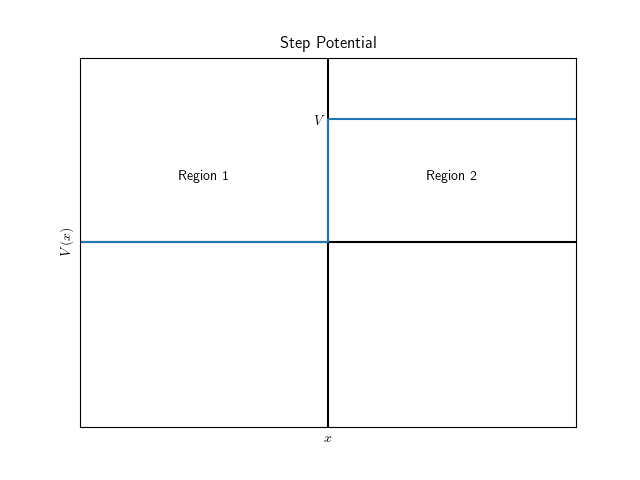
\includegraphics[scale=0.6]{step_potential.png}
        \caption{The step potential}
    \end{figure}
    
    \subsubsection{Case 1: \texorpdfstring{\(E > V\)}{E > V}}
    Classically we would expect a particle incident from the left with \(E > V\) to enter region 2, \(x > 0\).
    Since the total energy of the particle is constant and given by \(H = T + V\) then we would expect that upon entering region 2 the kinetic energy, and hence momentum, of the classical particle will have to decrease to keep the total energy constant.
    
    The \gls{tise} can be split into two section, in region 1, \(x < 0\), we have
    \[-\frac{\hbar^2}{2m}\dv[2]{x}\psi(x) = E\psi(x) \implies \psi''(x) = -\frac{p^2}{\hbar^2}\psi(x)\]
    where
    \[p = \sqrt{2mE},\]
    this is exactly the momentum of a classical particle with energy \(E\) and a potential energy of 0.
    In region 2 we have
    \[\left[-\frac{\hbar^2}{2m}\dv[2]{x}+ V\right]\psi(x) = E\psi(x) \implies \psi''(x) = -\frac{\bar{p}}{\hbar^2}\psi(x)\]
    where
    \[\bar{p} = \sqrt{2m(E - V)},\]
    this is exactly the momentum of a classical particle with energy \(E\) and a potential energy of \(V\).
    As we would expect the momentum in region 2, \(\bar{p}\), is less than the momentum in region 1, \(p\).
    Fortunately we already know the solution to the wave equation in both regions:
    \[
        \psi(x) =
        \begin{cases}
            Ae^{ipx/\hbar} + Be^{-ikp/\hbar}, &x < 0,\\
            Ce^{i\bar{p}x/\hbar} + De^{-i\bar{p}x/\hbar} &x > 0.
        \end{cases}
    \]
    The solutions are a superposition of waves with momentum \(\pm p\) and \(\pm\bar{p}\) in the respective region.
    By `wave with momentum \(p\)' we mean a wave function such that \(p\) is an eigenvalue of \(\operator{P}\).
    
    Suppose that a particle comes in from the left.
    Then we expect a wave propagating to the right in both regions and a wave propagating to the left in region 1 corresponding to the wave reflecting off the boundary.
    However there is no reason to expect a wave propagating left in region 2 as once the wave enters that region there is nothing to cause a reflection.
    Therefore \(D = 0\).
    
    We are left with three degrees of freedom, \(A\), \(B\), and \(C\).
    We can fix one by requiring a normalised wave function, say we choose \(A\) for this purpose.
    We then use the requirements of continuity of \(\psi\) and \(\psi'\) to fix the other two degrees of freedom.
    Clearly \(\psi\) and \(\psi'\) are continuous at all \(x \ne 0\) so we only need to consider continuity at \(x = 0\).
    We require that
    \[\lim_{x\to0^+}\psi(x) = \lim_{x\to0^-}\psi(x),\]
    and
    \[\lim_{x\to0^+}\psi'(x) = \lim_{x\to0^-}\psi'(x).\]
    The first of these gives us
    \[\lim_{x\to0^+}\psi(x) = \lim_{x\to0^+}\left[Ae^{ipx/\hbar} + Be^{-ikx/\hbar}\right] = A + B\]
    \[\lim_{x\to0^-}\psi(x) = \lim_{x\to0^-} Ce^{i\bar{p}x/\hbar} = C.\]
    Hence
    \[A + B = C.\]
    The second leads to 
    \[\lim_{x\to0^+}\psi'(x) = \lim_{x\to0^+}\left[\frac{ip}{\hbar}Ae^{ipx/\hbar} - \frac{ip}{\hbar}Be^{-ikx/\hbar}\right] = \frac{ip}{\hbar}A + \frac{ip}{\hbar}B\]
    \[\lim_{x\to0^-}\psi'(x) = \lim_{x\to0^-} \frac{i\bar{p}}{\hbar}Ce^{i\bar{p}x/\hbar} = \frac{i\bar{p}}{\hbar}C.\]
    Hence
    \[p(A + B) = \bar{p}C.\]
    We can then show that
    \[B = \frac{p - \bar{p}}{p + \bar{p}}A,\qquad\text{and}\qquad C = \frac{2p}{p + \bar{p}}A.\]
    This imposes no restrictions on the energy, \(E\) can take any value as long as it is greater than \(V\).
    The Hamiltonian has a continuous spectrum.
    Notice that in general \(B \ne 0\) so there is a reflected wave going left in region 1.
    
    \subsubsection{Case 2: \texorpdfstring{\(E < V\)}{E<V}}
    The situation is very similar if \(E < V\) but now region 2 is classically forbidden, meaning that a classical particle could not enter into this region.
    The equations for the wave function are the same but since \(E < V\) \(E - V\) is now negative meaning that \(\bar{p}\) is imaginary:
    \[\bar{p} = \sqrt{2m(E - V)} = i\sqrt{2m(V -  E)} = i\tilde{p}.\]
    In region 2 the solution to the wave function is now
    \[\psi(x) = Ce^{-\tilde{p}x/\hbar} + De^{\tilde{p}x/\hbar}.\]
    The first term is a decaying exponential and is finite in region 2.
    The second is an increasing exponential and therefore goes to infinity as \(x \to\infty\).
    This is not allowed so we discard this term in order for \(\psi\) to be normalisable.
    Hence in region 2
    \[\psi(x) = Ce^{-\tilde{p}x/\hbar}.\]
    Region 2 is classically forbidden but the wave function is non-zero in region 2 therefore there is a non-zero probability that the particle will be found in region 2.
    This time we can show that
    \[B = \frac{p - i\tilde{p}}{P + i\tilde{p}}A.\]
    The fraction here has unit modulus so we must have that \(\abs{B}^2 = \abs{A}^2\), this means that they just differ by a phase, \(\delta\):
    \[B = e^{-2i\delta(E)}A,\]
    here we emphasise the fact that \(\delta\) is a function of the energy (not the Dirac delta).
    It can also be shown that
    \[\tilde{p} = p\cot\delta.\]
    We define \(\lambda\) as the length that the particle penetrates the classically forbidden region and we note that it scales as \(\hbar/p\).
    
    \subsection{Potential Barrier}
    Consider the potential
    \[
        V(x) = 
        \begin{cases}
            V, & x \in [0, a],\\
            0, & x\notin[0, a],
        \end{cases}
    \]
    \begin{figure}[ht]
        \centering
        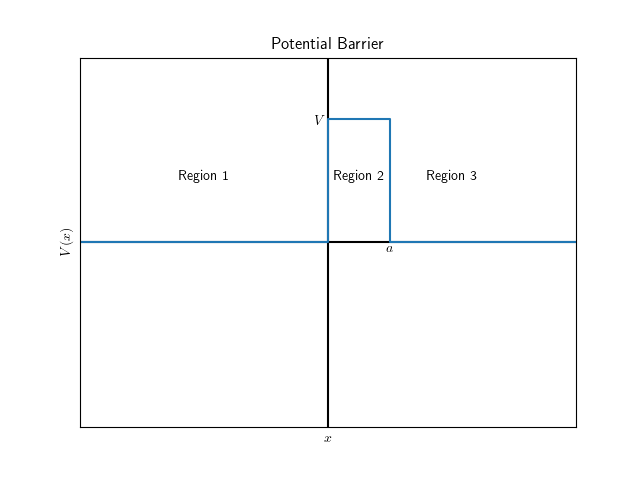
\includegraphics[scale=0.6]{potential_barrier.png}
        \caption{The potential barrier}
    \end{figure}
    for some positive constant, \(V\).
    Again there are two cases, \(E > V\) and \(E < V\).
    In the cases that \(E > V\) this is very similar to the same case with the potential step.
    The wave function will be oscillatory in all three regions with an amplitude that depends on the value of the potential.
    The interesting case is when \(E < V\).
    
    Classically when \(E < V\) region 2 is forbidden.
    A particle entering from the left has no way to go past the origin, it will reflect off the origin and go back to \(-\infty\).
    The solution to the Schr\"odinger equation is
    \[
        \psi(x) =
        \begin{cases}
            Ae^{ipx/\hbar} + Be^{ipx/\hbar}, & x \in (-\infty, 0),\\
            Ce^{-\tilde{p}x/\hbar} + De^{\tilde{p}x/\hbar}, &x \in (0, a),\\
            Fe^{ipx/\hbar} + Ge^{ipx/\hbar}, & x \in (a, \infty).
        \end{cases}
    \]
    Here \(p\) and \(\tilde{p}\) are defined as they were for the potential step.
    Notice that since \(x\) is finite in \((0, a)\) there is no reason to discard the term \(De^{\tilde{p}x/\hbar}\) as it is finite for all \(x\in(0, a)\).
    For the same reason as before if we have a particle coming in from the left we must have that \(G = 0\).
    So in region 3
    \[\psi(x) = Fe^{ipx/\hbar} = AS(E)e^{ip(x - a)/\hbar}.\]
    The last part of this is the conventional way to write this term.
    Of particular interest is \(S(E)\), this is the ratio of the probability amplitude of the wave entering the barrier at \(x = 0\), to the probability amplitude of the wave leaving the barrier at \(x = a\).
    \(S(E)\) can be shown to be
    \[S(E) = \frac{2ip\tilde{p}}{(p^2 - \tilde{p}^2)\sinh(\tilde{p}a/\hbar) + 2ip\tilde{p}\cosh(\tilde{p}a/\hbar)}.\]
    The transmissivity, \(T\), is defined as the probability that the particle tunnels through the barrier, that is
    \[T = \abs{S(E)}^2 = \left[1 + \frac{\sinh^2(\tilde{p}a/\hbar)}{4(E/V)(1 - E/V)}\right]^{-1}.\]
    For \(E < V\) this is a monotonically increasing function of \(E\) for a fixed value of \(a\).
    This means that as the energy increases the probability that the particle tunnels through the barrier increases.
    Importantly
    \[T \propto e^{-ka}\]
    for some constant \(k\).
    Therefore as \(a\) increases for a fixed value of \(E\) the probability that the particle tunnels into region 3 decreases.
    
    \subsubsection{Tunnelling}
    Tunnelling is a phenomenon without classical analogue.
    It can be experimentally verified and is one of many confirmations that quantum mechanics yields correct predictions.
    Tunnelling has many applications in physics.
    
    The process of alpha decay can be seen as a process of the alpha particle tunnelling out of a potential well created by the nucleus.
    Figure~\ref{fig:alpha decay} shows a phenomenological potential used to model alpha decay.
    The alpha particle is in a potential well and typically has less energy than the maximum potential.
    However it is still possible for the alpha particle to tunnel out of the well, and out of the nucleus.
    \begin{figure}[ht]
        \centering
        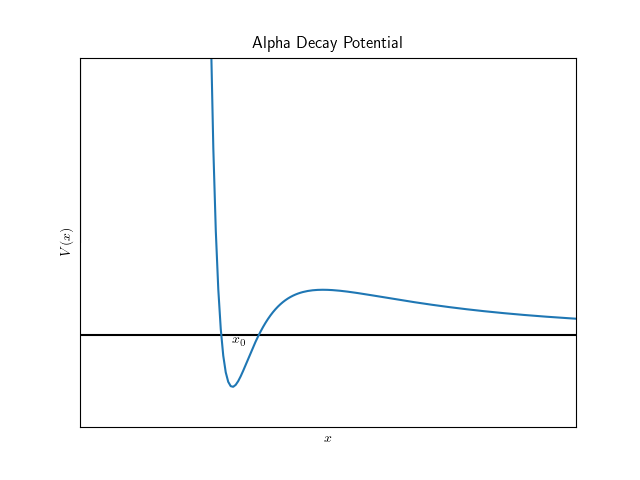
\includegraphics[scale=0.6]{alpha_decay.png}
        \caption{The potential modelling the alpha decay process. An alpha particle in the nucleus is in the potential well at \(x_0\), it can then tunnel outside of this well to some positive \(x\) value even if it has less energy than the peak on the right of the potential well.}
        \label{fig:alpha decay}
    \end{figure}

    \subsubsection{Scanning Tunnelling Microscope}
    A \gls{stm} is made of a needle that is placed near the surface of a material.
    A current of electrons is applied to the needle.
    We can model the air gap between the needle point and the surface as a potential barrier.
    The electrons tunnel across this gap and a current flows.
    The current is proportional to the probability of an electron tunnelling so
    \[I \propto e^{-ka}.\]
    This allows for very small changes in the size of the air gap to be measured accurately by measuring the current.
    Scanning the \gls{stm} over the whole surface we can build up a picture of the 3-dimensional structure of the surface.
    
    \subsection{Infinite Potential Well}\label{sec:infinite square well}
    An infinite potential well of width \(a\) is a potential,
    \[
        V(x) =
        \begin{cases}
            0, & x \in(-a/2, a/2)\\
            \infty, & x\notin (-a/2, a/2).
        \end{cases}
    \]
    We are looking for the solutions to the \gls{tise} with positive energy (as the minimum potential is zero and the energy must be at least as large as this).
    We can view each boundary at \(\pm a/2\) as a potential step and then let \(V\to\infty\).
    The solution in these regions is
    \[\psi \sim e^{-\tilde{p}\delta/\hbar}.\]
    For finite \(V\)
    \[\tilde{p} = \sqrt{2m(V - E)}.\]
    As \(V\to\infty\) \(\tilde{p} \to \infty\) and so \(\psi\to 0\).
    We see that the regions outside of the well are not only classically forbidden but completely inaccessible, even to a quantum particle.
    
    Therefore we only need to solve the \gls{tise} in the region \((-a/2, a/2)\) and apply boundary conditions at \(x = \pm a/2\).
    The boundary conditions here are \(\psi(\pm a/2) = 0\) as we require continuity of \(\psi\).
    Note that since \(V\) is not finite we do not require continuity of \(\psi'\).
    The general form of the solution in the well is that of a free particle:
    \[\psi(x) = Ae^{ikx} + Be^{-ikx}\]
    where \(k = p/\hbar\) and \(p = \sqrt{2mE}\) is the classical momentum.
    At the boundaries we have
    \[\psi(a/2) = Ae^{ika/2} + Be^{-ika/2} = 0 \implies B = -Ae^{ika},\]
    substituting this into the second boundary condition we have
    \begin{align*}
        \psi(-a/2) &= Ae^{-ika/2} - Ae^{ika}e^{ika/2}\\
        &= Ae^{ika/2}(e^{-ika} - e^{ika})\\
        &= Ae^{ika/2}[\cos(ka) - i\sin(ka) - \cos(ka) - i\sin(ka)]\\
        &= 2iAe^{ika/2}\sin(ka).
    \end{align*}
    We require this to be zero.
    Since \(2iAe^{ika/2}\ne 0\) (assuming \(A\) is non-zero, as it must be for any wave function of interest) we must have that \(\sin(ka) = 0\).
    Therefore
    \[ka = n\pi \implies k = \frac{n\pi}{a},\qquad n\in\naturals.\]
    From this we have
    \[\frac{n\pi}{a} = k = \frac{p}{\hbar} = \frac{\sqrt{2mE}}{\hbar} \implies E = \frac{n^2\pi^2\hbar^2}{2ma^2}.\]
    Since \(n\in\naturals\) the energy, \(E\), is quantised.
    From now on we will denote the energy of the \(n\)th state as
    \[E_n = \frac{1}{2m}\left(\frac{\hbar\pi n}{a}\right)^2.\]
    If we normalise the wave functions we find that the properly normalised eigenstates of the Hamiltonian are
    \[
        u_n =
        \begin{cases}
            \sqrt{\frac{2}{a}}\sin\left(\frac{n\pi x}{a}\right), & n~\text{even},\\
            \sqrt{\frac{2}{a}}\cos\left(\frac{n\pi x}{a}\right), & n~\text{odd}.
        \end{cases}
    \]
    Since \(u_n(x) = 0\) is boring we consider \(u_1\) to be the ground state.
    In this state the particle is most likely to be found at \(x = 0\).
    The first four wave functions, and the associated probability densities, are shown in figure~\ref{fig:infinite square well wave functions}.
    \begin{figure}[ht]
        \centering
        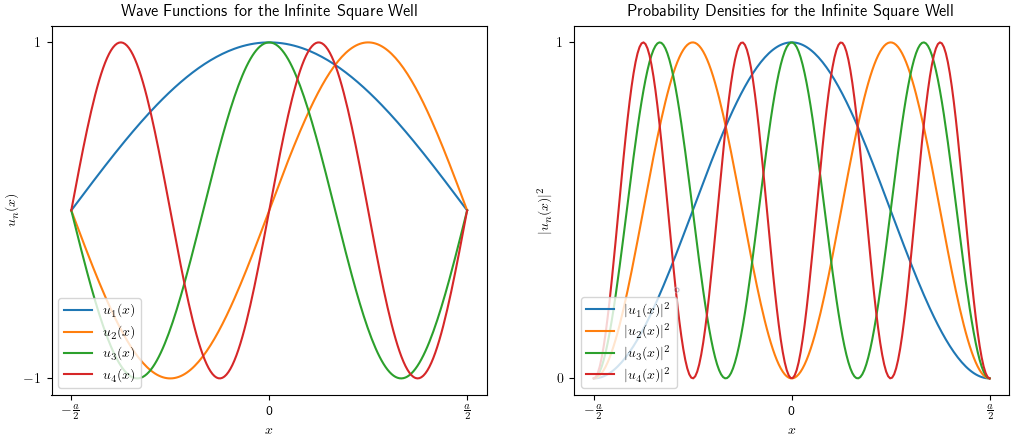
\includegraphics[scale=0.5]{infinite_square_well_wave_func.png}
        \caption{The first four wave functions, \(u_n\), for the infinite square well and the the associated probability densities.}
        \label{fig:infinite square well wave functions}
    \end{figure}
    The generic state of a particle in an infinite square well potential is a linear combination of \(\{u_n(x)\}\).
    That is a linear superposition of eigenstates of \(\operator{P}\) with eigenvalues
    \[\pm p_n = \pm \hbar k_n = \pm\frac{n\pi\hbar}{a}.\]
    
    \subsubsection{Zero Point Energy}
    Notice that in the ground state \(p_1 = \pi\hbar/a \ne 0\).
    This can be seen as a direct consequence of \gls{hup}.
    Since the particle is constrained to have \(x\in(-a/2, a/2)\) this gives us a maximum uncertainty in \(x\) of \(\Delta x = a\).
    Hence
    \[\Delta p\Delta x \ge \frac{\hbar}{2} \implies \Delta p \ge \frac{\hbar}{2a}.\]
    Therefore the momentum cannot be zero, as then we would know the value with zero uncertainty, which is certainly less than \(\hbar/2a\).
    The energy in this state is consequently also non-zero:
    \[E \sim \frac{(\Delta p)^2}{2m} \ge \frac{\hbar^2}{8ma}.\]
    The kinetic energy due to the uncertainty principle is called the zero point energy.
    One consequence of this is that helium can be a liquid at \(T = \SI{0}{\kelvin}\).
    This is because in order to form a solid the atoms must be constrained to a lattice giving them some non-zero zero point energy, which scales inversely to the mass, for a particle as light as helium it is enough to overcome interatomic forces and the system remains in a liquid phase.
    
    \subsubsection{Symmetry of the Solutions}
    The energy eigenstates have definite parity, that is if we define the parity operator, \(\operator{\parity}\), to have the action
    \[\operator{\parity}\psi(x) = \psi(-x),\]
    then the energy eigenstates are also eigenstates of the parity operator:
    \[\operator{\parity}u_n(x) = (-1)^{n+1}u_n(x).\]
    This can be seen from the explicit form of \(u_n\) and using the fact that sine and cosine are odd and even functions respectively.
    This means that \(u_n\) are simultaneously eigenfunctions of \(\operator{\parity}\), \(\operator{P}\), and \(\operator{H}\).
    
    We can show that in general if the potential is symmetric, so \(V(-x) = V(x)\), then \([\operator{H}, \operator{\parity}] = 0\), that is \(\operator{H}\) is symmetric under \(\operator{\parity}\).
    This then implies the existence of a basis of simultaneous eigenstates of \(\operator{H}\) and \(\operator{\parity}\).
    
    It is fairly simple to show the above paragraph is true.
    Suppose that \(V\) is a symmetric potential.
    Then
    \begin{align*}
        \operator{\parity}\operator{H}\psi(x) &= \operator{\parity}\left[-\frac{\hbar^2}{2m}\dv[2]{x} + V(x)\right]\psi(x)\\
        &= \operator{\parity}\left[-\frac{-\hbar^2}{2m}\dv[2]{\psi(x)}{x} + V(x)\psi(x)\right]\\
        &= -\frac{\hbar^2}{2m}\dv[2]{\psi(-x)}{x} + V(-x)\psi(-x)\\
        &= -\frac{\hbar^2}{2m}\dv[2]{\psi(-x)}{x} + V(x)\psi(-x).
     \end{align*}
    Here we have used the fact that
    \[\operator{\parity}\dv{x} = \dv{-x} = -\dv{x}\]
    and hence
    \[\operator{\parity}\dv[2]{x} = -\dv{x}\left(-\dv{x}\right) = \dv[2]{x}.\]
    Also
    \begin{align*}
        \operator{H}\operator{\parity}\psi(x)& = \operator{H}\psi(-x)\\
        &= \left[-\frac{\hbar^2}{2m}\dv[2]{x} + V(x)\right]\psi(-x)\\
        &= -\frac{\hbar^2}{2m}\dv[2]{\psi(-x)}{x} + V(x)\psi(-x).
    \end{align*}
    Hence
    \[[\operator{\parity}, \operator{H}] = 0.\]
    We know that this means there is a common basis of eigenstates but how do we find it?
    The states
    \[v_n^+(x) = u_n(x) + u_n(-x),\qquad\text{and}\qquad v_n^-(x) = u_n(x) - u_n(-x)\]
    are one such basis.
    These states can be compactly written as
    \[v_n^{\pm}(x) = (1 \pm \operator{\parity})u_n(x).\]
    It is then easy to show that these are eigenstates of \(\operator{H}\) and \(\operator{\parity}\):
    \begin{multline*}
        \operator{H}v_n^{\pm}(x) 
        = \operator{H}(1 \pm \operator{\parity})u_n(x) 
        = \operator{H}u_n(x) \pm \operator{H}\operator{\parity}u_n(x) 
        = \operator{H}u_n(x) \pm \operator{\parity}\operator{H}u_n(x) \\
        = E_nu_n(x) + E_n\operator{\parity}u_n(x) 
        = E_n(1 \pm \operator{\parity})u_n 
        = E_nv_n^{\pm}(x).
    \end{multline*}
    and
    \begin{multline*}
        \operator{\parity}v_n^{\pm}(x) 
        = \operator{\parity}(1 \pm \operator{\parity})u_n(x)
        = \operator{\parity}u_n(x) \pm \operator{\parity}^2u_n(x)
        = \operator{\parity}u_n(x) \pm (-1)^{n+1}(-1)^{n+1}u_n(x)\\ 
        = \operator{\parity}u_n(x) \pm u_n(x)
        = \operator{\parity}u_n(x) \pm u_n(x)
        = \pm(1 \pm \operator{\parity})u_n(x)
    \end{multline*}

    \subsection{Finite Potential Well}
    The finite potential well has the potential
    \[
        V(x) = 
        \begin{cases}
            -V_0, & x\int(-a/2, a/2),\\
            0, & x\notin(-a/2, a/2),
        \end{cases}
    \]
    for some positive constant \(V_0\).
    This potential is symmetric under parity change.
    This means that we can look for a set of energy eigenstates that are also parity eigenstates.
    The energy eigenvalues must be greater than \(-V_0\).
    States with \(-V_0 < E < 0\) are called \define{bound states}.
    The wave function for these states decays exponentially for \(\abs{x} > a/2\) so the probability of finding the particle outside of the well becomes small quickly.
    The states with \(E > 0\) are simply plane waves that have a momentum change and chance of reflection at each boundary, this isn't that interesting and is just like the potential step so we won't consider these states further.
    
    The Schr\"odinger equation is
    \[
        \psi''(x) = 
        \begin{cases}
            -\frac{2m}{\hbar^2}E\psi(x), & \abs{x} > a/2,\\
            -\frac{2m}{\hbar^2}(E + V_0)\psi(x), & \abs{x} < a/2.
        \end{cases}
    \]
    Unlike the infinite well the wave function is non-zero outside the well.
    For \(-V_0 < E < 0\) the even parity solutions are
    \[
        \psi(x) =
        \begin{cases}
           A\cos(px/\hbar), & \abs{x} < a/2,\\
           Ce^{-\bar{p}x/\hbar}, & x > a/2,\\
           Ce^{\bar{p}x/\hbar}, & x < -a/2.
        \end{cases}
    \]
    The odd parity solutions are
    \[
        \psi(x) =
        \begin{cases}
            A\sin(px/\hbar), & \abs{x} < a/2,\\
            Ce^{-\bar{p}x/\hbar}, & x > a/2,\\
            -Ce^{\bar{p}x/\hbar}, & x < -a/2.
        \end{cases}
    \]
    We have introduced the momenta
    \[p = \sqrt{2m(E + V_0)},\qquad\text{and}\qquad \bar{p}\sqrt{-2mE}.\]
    There are two things to notice here, first \(-V_0 < E < 0\) so \(p, \bar{p}\in\reals\), and here the factor of \((E + V_0)\) appears in \(p\) whereas previously it appeared in \(\bar{p}\).
    The reason for this is that previously we viewed the minimum of the potential as \(0\) and the maximum as \(V\) but here the minimum is \(-V_0\) and the maximum is \(0\).
    
    Imposing continuity at \(a/2\) in both the wave function and its derivative we have for the even solutions that
    \begin{align*}
        A\cos\left(\frac{pa}{2\hbar}\right) &= Ce^{-\bar{p}a/2\hbar}\\
        -\frac{p}{\hbar}A\sin\left(\frac{pa}{2\hbar}\right) &= -\frac{\bar{p}a}{\hbar}Ce^{-\bar{p}a/2\hbar}.
    \end{align*}
    Dividing the first equation by the second we get the quantisation condition
    \[p\tan\left(\frac{pa}{2\hbar}\right) = \bar{p}.\]
    Similarly for the odd parity solutions we have
    \begin{align*}
        A\sin\left(\frac{pa}{2\hbar}\right) &= Ce^{-\bar{p}a/2\hbar}\\
        \frac{p}{\hbar}A\cos\left(\frac{pa}{2\hbar}\right) &= -\frac{\bar{p}a}{\hbar}Ce^{-\bar{p}a/2\hbar}.
    \end{align*}
    This leads to
    \[p\cot\left(\frac{pa}{2\hbar}\right) = -\bar{p}.\]
    There is always at least one even bound state.
    For small \(V_0\), corresponding to a shallow well, it can be shown that
    \[E = -\frac{mV_0^2a^2}{2\hbar^2}\]
    for the ground state.
    
    \section{Harmonic Oscillators}
    \subsection{The Classical Harmonic Oscillators}
    The equation of motion for a classical particle of mass \(m\) undergoing one-dimensional harmonic oscillations, undergoing a restoring force proportional to the displacement, is
    \[m\ddot{x} = -kx.\]
    The constant \(k\) is often called the spring constant due to the common example of a mass on a spring where this is exactly what \(k\) is.
    The solution is oscillatory with an angular frequency
    \[\omega = \sqrt{\frac{k}{m}}.\]
    Using the chain rule we have
    \[\ddot{x} = \dv[2]{x}{t} = \dv{v}{t} = \dv{v}{x}\dv{x}{t} = v\dv{v}{x}.\]
    Integrating the equation of motion we then have
    \[m\int v\dv{v}{x}\dd{x} = -k\int x\dd{x} \implies \frac{1}{2}mv^2 = -\frac{1}{2}kx^2 + E\]
    where \(E\) is the total energy of the system, which appears as a constant of integration.
    Thus
    \[\frac{1}{2}mv^2 + \frac{1}{2}kx^2 = E.\]
    Identifying the first term as the kinetic energy we see that the potential energy is
    \[V(x) = \frac{1}{2}kx^2 = \frac{1}{2}m\omega^2x^2.\]
    The total energy is
    \[E = \frac{1}{2}m\omega^2L^2\]
    where \(L\) is the amplitude of the oscillations.
    It is easy to show that this is the maximum energy by noting that at \(x = L\) the particle is instantaneously stationary as it changes direction so the kinetic energy is zero.
    
    \subsection{The Quantum Harmonic Oscillator}
    The transformation to the quantum case is straight forward.
    The potential is simply
    \[V(\operator{X}) = \frac{1}{2}m\omega^2\operator{X}^2.\]
    Assuming a discrete spectrum we have to solve the \gls{tise}:
    \[\operator{H}\ket{n} = E_n\ket{n},\]
    where
    \[\operator{H} = \frac{\operator{P}^2}{2m} + \frac{1}{2}m\omega^2\operator{X}^2.\]
    Taking the inner product of the \gls{tise} with an eigenstate of \(\operator{X}\) we have
    \[\bra{x}\operator{H}\ket{n} = E_n\braket{x}{n} = E_nu_n(x)\]
    defining \(u_n(x) = \braket{x}{n}\) as the energy eigenfunction with energy \(E_n\).
    The full \gls{tise} is then
    \[\left[-\frac{\hbar^2}{2m}\dv[2]{x} + \frac{1}{2}m\omega^2 x^2\right]u_n(x) = E_nu_n(x).\]
    
    \subsection{The Solutions to the Harmonic Oscillator}
    We will start by discussing the solutions to this and look at deriving them in later sections.
    The first thing to note is that the energy is quantised as follows:
    \[E_n = \left(n + \frac{1}{2}\right)\hbar\omega,\qquad\text{where}\qquad n\in\naturals.\]
    The ground state corresponds to \(n = 0\) and has the non-zero energy \(E_0 = \hbar\omega/2\).
    The energy eigenfunctions are
    \[u_n(x) = C_ne^{-\alpha^2x^2/2}H_n(\alpha x).\]
    Here \(C_n\) is a normalisation constant, \(\alpha^2 = m\omega/\hbar\) and \(H_n\) are polynomials of degree \(n\) called the \define{Hermite polynomials}.
    The Hermite polynomials are orthogonal in such that
    \[\int_{-\infty}^{\infty} \dd{s}e^{-s^2}H_m(s)H_n(s) = 2^n\sqrt{\pi}n!\delta_{mn},\]
    which is only non-zero if \(n = m\).
    The first four Hermite polynomials are
    \begin{align*}
        H_0(s) &= 1,  & H_2(s) &= 4s^2 - 2,\\
        H_1(x) &= 2s, & H_3(s) &= 8s^3 - 12s.
    \end{align*}
    Note that if \(n\) is even (odd) then \(H_n(s)\) only contains even (odd) powers of \(s\), this is true for all \(n\).
    This means that the Hermite polynomials have even (odd) parity for even (odd) \(n\).
    Since the Gaussian term of \(u_n\) has even parity this means that the parity of \(u_n\) is the same as \(H_n\).
    That is
    \[\operator{\parity}u_n(x) = u_n(-x) = (-1)^nu_n(x).\]
    We see that the energy eigenstates are eigenstates of the parity operator, \(\operator{\parity}\), which is a direct consequence of the potential being symmetric:
    \[V(-x) = \frac{1}{2}m\omega^2(-x)^2 = \frac{1}{2}m\omega^2x^2 = V(x).\]
    Since \(u_n\) has definite parity \(\abs{u_n(x)}^2\) is even.
    Therefore
    \[\expected{x}_n = \bra{n}\operator{X}\ket{n} = \int_{-\infty}^{\infty} \dd{x} x\abs{u_n(x)}^2 = 0,\]
    as the integrand is always odd and an integral of an odd function over an even interval, \((-\infty, \infty)\), is zero.
    Strictly speaking this only holds if the integral converges but in this case it clearly does as the Gaussian part goes to zero much faster than the polynomial parts can go to infinity.
    A quick sanity check here would be to think about the potential and since it is symmetric the particle is equally likely to be at a positive \(x\) as it is at a negative \(x\) and therefore the expected value should be zero.
    
    The next quantity that we might want to compute is the expected value of \(x^2\) which is
    \[\expected{x^2}_n = \int_{-\infty}^{\infty} \dd{x} x^2\abs{u_n(x)}^2 = \left(n + \frac{1}{2}\right)\frac{1}{\alpha^2}.\]
    From this we can see that for larger energies it becomes more probable to find the particle at large \(x\), that is the variance, \(\Delta x_n = \expected{x}_n - \expected{x}_n^2 = \expected{x^2}_n\), increases with energy:
    \[E_n = m\omega^2\expected{x^2}_n.\]
    Compare this to the classical energy,
    \[E = \frac{1}{2}m\omega^2L^2.\]
    
    \subsection{Solving the Harmonic Oscillator (The Fancy Way)}
    \subsubsection{Factorising the Hamiltonian}
    The Hamiltonian is
    \[\operator{H} = \frac{\operator{P}^2}{2m} + \frac{1}{2}m\omega^2\operator{X}^2.\]
    We can factor out \(\hbar\omega\) from this:
    \[\operator{H} = \hbar\omega\left[\frac{1}{2m\hbar\omega}\operator{P}^2 + \frac{m\omega}{2\hbar}\operator{X}^2 \right].\]
    Since \(\hbar\omega\) has units of energy the term in the brackets must be dimensionless.
    We define two operators
    \[\operator{\xi} = \sqrt{\frac{m\omega}{2\hbar}}, \qquad\text{and}\qquad \operator{\eta} = \frac{1}{\sqrt{2m\hbar\omega}}\operator{P}.\]
    These are simply rescaled, dimensionless, versions of the position and momentum operators.
    The Hamiltonian can now be written as
    \[\operator{H} = \hbar\omega[\operator{\xi}^2 + \operator{\eta}^2].\]
    Since \(\operator{\xi}\) and \(\operator{\eta}\) are proportional to the position and momentum operators we know that they don't commute, in fact their commutator is
    \begin{align*}
        [\operator{\xi}, \operator{\eta}] &= \sqrt{\frac{m\omega}{2\hbar}}\frac{1}{\sqrt{2m\hbar\omega}} [\operator{X}, \operator{P}]\\
        &= \frac{1}{2\hbar}[\operator{X}, \operator{P}]\\
        &= \frac{i}{2}.
    \end{align*}
    There are two checks that it is good to do here.
    First since \(\operator{\xi}\) and \(\operator{\eta}\) are dimensionless their commutator should be too, and it is.
    Second since \(\operator{X}\) and \(\operator{P}\) are Hermitian then so are \(\operator{\xi}\) and \(\operator{\eta}\) and therefore their commutator should be anti-Hermitian, and it is.
    
    We now define a new operator:
    \[\operator{a} = \operator{\xi} + i\operator{\eta},\qquad\text{and}\qquad \operator{a}\hermit = \operator{\xi} - i\operator{\eta}.\]
    The motivation behind this is that if \(\operator{\xi}\) and \(\operator{\eta}\) commuted then we could factorise the Hamiltonian as
    \[\hbar\omega(\operator{\xi} + i\operator{\eta})(\operator{\xi} - i\operator{\eta}).\]
    However we cannot do this.
    We can write this new operator in terms of \(\operator{X}\) and \(\operator{P}\):
    \begin{align*}
        \operator{a} &= \sqrt{\frac{m\omega}{2\hbar}} \operator{X} + \frac{i}{\sqrt{2m\omega\hbar}} \operator{P} = \sqrt{\frac{m\omega}{2\hbar}}\left[\operator{X} + \frac{i}{m\omega}\operator{P}\right]\\
        \operator{a}\hermit &= \sqrt{\frac{m\omega}{2\hbar}} \operator{X} - \frac{i}{\sqrt{2m\omega\hbar}} \operator{P} = \sqrt{\frac{m\omega}{2\hbar}}\left[\operator{X} - \frac{i}{m\omega}\operator{P}\right]\\
    \end{align*}
    We can then compute
    \begin{align*}
        \operator{a}\operator{a}\hermit &= (\operator{\xi} + i\operator{\eta})(\operator{\xi} - i\operator{\eta})\\
        &= \operator{\xi}^2 + i\operator{\eta}\operator{\xi} - i\operator{\xi}\operator{\eta} + \operator{\eta}^2\\
        &= \operator{\xi} + i[\operator{\eta}, \operator{\xi}] + \operator{\eta}^2,
    \end{align*}
    and
    \begin{align*}
        \operator{a}\hermit\operator{a} &= (\operator{\xi} - i\operator{\eta})(\operator{\xi} + i\operator{\eta})\\
        &= \operator{\xi}^2 + i\operator{\xi}\operator{\eta} - i\operator{\eta}\operator{\xi} + \operator{\eta}^2\\
        &= \operator{\xi}^2 - i[\operator{\eta}, \operator{\xi}] + \operator{\eta}^2.
    \end{align*}
    Subtracting these two equations we have
    \[[\operator{a}, \operator{a}\hermit] = 1,\]
    and adding the equations we have
    \[\operator{H} = \frac{1}{2}\hbar\omega(\operator{a}\operator{a}\hermit + \operator{a}\hermit\operator{a}).\]
    A more useful form for the Hamiltonian can be found by adding zero:
    \[\operator{H} = \frac{1}{2}\hbar\omega(\operator{a}\operator{a}\hermit + \operator{a}\hermit\operator{a}) = \frac{1}{2}\hbar\omega(\operator{a}\operator{a}\hermit - \operator{a}\hermit\operator{a} + \operator{a}\hermit\operator{a}+ \operator{a}\hermit\operator{a}) = \frac{1}{2}\hbar\omega([\operator{a}, \operator{a}\hermit] + 2\operator{a}\hermit\operator{a}) = \hbar\omega\left(\operator{a}\hermit\operator{a} + \frac{1}{2}\right).\]
    
    \subsubsection{Creation and Annihilation}
    For this section we will need the commutators of \(\operator{a}\) and \(\operator{a}\hermit\) with the Hamiltonian, fortunately these are fairly easy to compute now:
    \[[\operator{H}, \operator{a}] = \left[\hbar\omega\left(\operator{a}\hermit \operator{a} + \frac{1}{2}\right), \operator{a}\right] = \hbar\omega[\operator{a}\hermit\operator{a}, \operator{a}]\]
    using the fact that \([1/2, \operator{a}] = 0\).
    Then
    \[[\operator{a}\hermit\operator{a}, \operator{a}] = \operator{\hermit}\operator{a}\operator{a} - \operator{a}\operator{a}\hermit\operator{a} = [\operator{a}\hermit, \operator{a}]\operator{a} = -\operator{a}.\]
    Therefore
    \[[\operator{H}, \operator{a}] = \hbar\omega [\operator{a}\hermit\operator{a}, \operator{a}] = -\hbar\omega\operator{a.}\]
    Similarly
    \[[\operator{H}, \operator{a}\hermit] = \left[\hbar\omega\left(\operator{a}\hermit \operator{a} + \frac{1}{2}\right), \operator{a}\hermit\right] = \hbar\omega[\operator{a}\hermit\operator{a}, \operator{a}\hermit] = \hbar\omega(\operator{a}\hermit\operator{a}\operator{a}\hermit - \operator{a}\hermit\operator{a}\hermit\operator{a}) = \hbar\omega\operator{a}\hermit[\operator{a}, \operator{a}\hermit] = \hbar\omega\operator{a}\hermit.\]
    Suppose \(\ket{n}\) is an energy eigenstate.
    We would like to know how \(\operator{a}\) acts on this since working in the energy eigenbasis we can then describe the action of \(\operator{a}\) on any state.
    To do this we will use that
    \[\operator{H}\operator{a} = \operator{a}\operator{H} + \operator{H}\operator{a} - \operator{a}\operator{H} = \operator{a}\operator{H} + [\operator{H}, \operator{a}].\]
    Thus
    \begin{align*}
        \operator{H}(\operator{a}\ket{n}) &= \operator{a}\operator{H}\ket{n} + [\operator{H}, \operator{a}]\ket{n}\\
        &= E_n\operator{a}\ket{n} - \hbar\omega\operator{a}\ket{n}\\
        &= (E_n - \hbar\omega)\operator{a}\ket{n}.
    \end{align*}
    So we see that \(\operator{a}\ket{n}\) is another eigenstate of \(\operator{H}\) with energy \(E_n - \hbar\omega\), unless \(\operator{a}\ket{n} = 0\).
    For this reason we say that \(\operator{a}\) is a \define{lowering operator} as its action is to return an eigenstate of lower energy.
    It is also called an \define{annihilation operator} as it annihilates one quantum of energy, \(\hbar\omega\), from the system.\footnote{\(\operator{a}\) and \(\operator{a}\hermit\) don't correspond to physical processes so we don't need to consider energy conservation.}
    Similarly
    \begin{align*}
        \operator{H}(\operator{a}\dagger\ket{n}) &= \operator{a}\operator{H}\ket{n} + [\operator{H}, \operator{a}\hermit]\\
        &= E_n\operator{a}\ket{n} + \hbar\omega\operator{a}\hermit\\
        &= (E_n + \hbar\omega)\operator{a}\hermit\ket{n}.
    \end{align*}
    So again \(\operator{a}\hermit\ket{n}\) is an energy eigenstate, this time with higher energy \(E_n + \hbar\omega\).
    We call \(\operator{a}\hermit\) a \define{raising operator} as its action is to return an eigenstate of higher energy.
    It is also called a \define{creation operator} as it adds one quantum of energy, \(\hbar\omega\), to the system.
    
    If \(\ket{n}\) is an energy eigenstate with energy \(E_n\) then define \(\ket{n\pm 1}\) to be an energy eigenstate with energy \(E_n \pm \hbar\omega\).
    Then
    \[\operator{a}\ket{n} = c_n\ket{n - 1},\qquad\text{and}\qquad \operator{a}\hermit\ket{n} = d_n\ket{n + 1}.\]
    Here \(c_n\) and \(d_n\) are constants of proportionality and not eigenvalues.
    
    By successive application of the annihilation operator, \(\operator{a}\), we can get states with lower and lower energy unless at some point \(\operator{a}\ket{0} = 0\) we call the state \(\ket{0}\) the ground state.
    Such a state must exist as the potential is bounded below and the energy is always at least as large as the minimum of the potential.
    We can find the ground state energy by applying the Hamiltonian:
    \[\operator{H}\ket{0} = \hbar\omega \left(\operator{a}\hermit\operator{a} + \frac{1}{2}\right)\ket{0} =  \hbar\omega\operator{a}\hermit\underbrace{\operator{a}\ket{0}}_{=0}\frac{\hbar\omega}{2}\ket{0} = \frac{\hbar\omega}{2}\ket{0}\]
    so we see that the ground state of the Harmonic oscillator has energy \(\hbar\omega/2\).
    
    Going the other way we can start from the ground state and construct states with progressively higher and higher energies by applying the creation operator, \(\operator{a}\hermit\).
    Unlike with the annihilation operator there is no reason that this should ever yield zero as the energy is in theory unbounded above.
    The first application of the creation operator gives
    \[\operator{a}\hermit \ket{0} = d_0\ket{1}\]
    where \(\ket{1}\) is a state with energy
    \[E_1 = \hbar\omega\left(1 + \frac{1}{2}\right) = \frac{3}{2}\hbar\omega.\]
    A second application gives
    \[\operator{a}\hermit{^2}\ket{0} = d_0\operator{a}\hermit\ket{1} = d_0d_1\ket{2}.\]
    At this point we see that we really need to know what \(c_n\) and \(d_n\) are.
    We find them by considering the expectation values of \(\operator{a}\hermit\operator{a}\) and \(\operator{a}\operator{a}\hermit\) and requiring all states be normalised:
    \begin{align*}
        \bra{n}\operator{a}\hermit\operator{a}\ket{n} &= c_n\bra{n}\operator{a}\hermit\ket{n - 1}\\
        &= c_n\bra{n-1}\operator{a}\ket{n}^*\\
        &= c_nc_n^*\braket{n-1}{n-1}\\
        &= \abs{c_n}^2.
    \end{align*}
    Also
    \[\operator{a}\hermit\operator{a} = \frac{1}{\hbar\omega}\operator{H} - \frac{1}{2}\]
    so
    \begin{align*}
        \bra{n}\operator{a}\hermit\operator{a}\ket{n} &= \frac{1}{\hbar\omega}\bra{n}\operator{H}\ket{n} - \frac{1}{2}\braket{n}{n}\\
        &= \frac{1}{\hbar\omega}E_n\braket{n}{n} - \frac{1}{2}\braket{n}{n}\\
        &= \frac{1}{\hbar\omega}\left(n + \frac{1}{2}\right)\hbar\omega  - \frac{1}{2}\\
        &= n
    \end{align*}
    Since states are only defined up to a phase factor we are free to choose \(c_n\) to be a real, positive, number so
    \[c_n = \sqrt{n}.\]
    For \(d_n\) consider
    \begin{align*}
        \bra{n}\operator{a}\operator{a}\hermit\ket{n} &= d_n \bra{n}\operator{a}\ket{n + 1}\\
        &= d_n\bra{n + 1}\operator{a}\hermit\ket{n}^*\\
        &= d_nd_n^*\braket{n + 1}{n + 1}
    \end{align*}
    Also
    \[\operator{a}\operator{a}\hermit = \frac{1}{\hbar\omega}\operator{H} + \frac{1}{2}\]
    so
    \begin{align*}
        \bra{n}\operator{a}\operator{a}\hermit\ket{n} &= \frac{1}{\hbar\omega}\bra{n}\operator{H}\ket{n} + \frac{1}{2}\braket{n}{n}\\
        &= \frac{1}{\hbar\omega}E_n\braket{n}{n} + \frac{1}{2}\braket{n}{n}\\
        &= \frac{1}{\hbar\omega}\left(n + \frac{1}{2}\right)\hbar\omega + \frac{1}{2}\\
        &= n + 1.
    \end{align*}
    So, again choosing \(d_n\) to be real and positive, we have
    \[d_n = \sqrt{n + 1}.\]
    So the full action of the raising and lowering operators is
    \[\operator{a}\ket{n} = \sqrt{n}\ket{n - 1},\qquad\text{and}\qquad \operator{a}\hermit\ket{n} = \sqrt{n + 1}\ket{n + 1}.\]
    We see that the action of \(\operator{a}\) on the ground state is
    \[\bra{x}\operator{a}\ket{0} = \bra{x}\sqrt{0}\ket{?} = 0\]
    for all \(\ket{x}\), as expected.
    
    \subsubsection{The Wave Function}
    We have introduced these creation and annihilation operators but we have yet to show that they allow us to find the correct wave functions for the system.
    We define \(\braket{x}{n} = u_n(x)\) and also we know for the ground state that \(\bra{x}\operator{a}\ket{0} = \operator{a}u_0(x) = 0\).
    We can also expand this with the definition of \(\operator{a}\) in terms of position and momentum operators:
    \begin{align*}
        0 &= \operator{a}u_0(x)\\
        &= \sqrt{\frac{m\omega}{2\hbar}}\left[\operator{X} + \frac{i}{m\omega}\operator{P}\right]u_0(x)\\
        &= \sqrt{\frac{m\omega}{2\hbar}}\left[x - \frac{i}{m\omega}i\hbar\dv{x}\right]u_0(x)\\
        \implies 0 &= xu_0(x) + \frac{\hbar}{m\omega}\dv{u_0}{x}\\
        \implies \dv{u_0}{x} &= -\frac{m\omega}{\hbar}xu_0(x)\\
        &= \alpha^2xu_0(x)\\
        \implies \frac{1}{u_0}\dv{u_0}{x} &= -\alpha x\\
        \implies \int \frac{1}{u_0}\dd{u_0} &= -\alpha^2 \int x \dd{x}\\
        \implies \ln(u_0) &= -\frac{1}{2}\alpha^2x^2 + \ln(N)
        \shortintertext{where \(\ln C\) is a constant of integration}
        \implies u_0 &= Ce^{-\alpha^2 x^2/2}.
    \end{align*}
    We can find \(C\) by requiring the state to be normalised so
    \begin{align*}
        1 &= \int_{-\infty}^{\infty} \abs{u_0(x)}^2 \dd{x}\\
        &= C^2 \int_{-\infty}^{\infty} e^{-\alpha^2x^2}\\
        &= C^2 \frac{\sqrt{\pi}}{\alpha}\\
        \implies C &= \frac{\sqrt{\alpha}}{\pi^{1/4}}.
    \end{align*}
    where we have used the standard result
    \[\int_{-\infty}^{\infty} e^{-p(x + q)^2} \dd{x} = \sqrt{\frac{\pi}{p}}.\]
    
    We can then construct any wave function by successive applications of \(\operator{a}\hermit\).
    However we must account for the constants of proportionality, for example
    \[\operator{a}\hermit{^4}\ket{0} = \sqrt{1}\operator{a}\hermit{^3}\ket{1} = \sqrt{1}\sqrt{2}\operator{a}\hermit{^2}\ket{2} = \sqrt{1}\sqrt{2}\sqrt{3}\operator{a}\hermit\ket{3} = \sqrt{1}\sqrt{2}\sqrt{3}\sqrt{4}\ket{4} = \sqrt{4!}\ket{4}.\]
    In general
    \[\ket{n} = \frac{1}{\sqrt{n!}}\operator{a}\hermit{^n}\ket{0}.\]
    Note that these states may still not be normalised as \(\operator{a}\hermit\) is not Hermitian so there is no guarantee that it preserves inner products.
    In terms of wave functions then we have
    \begin{align*}
        u_n(x) &= \frac{1}{\sqrt{n!}}\operator{a}\hermit{^n}u_0(x)\\
        &= \frac{1}{\sqrt{n!}}\left[\sqrt{\frac{m\omega}{2\hbar}} \left(\operator{X} - \frac{i}{m\omega}\operator{P}\right)\right]^nu_0(x)\\
        &= \frac{1}{\sqrt{n!}}\left[\sqrt{\frac{m\omega}{2\hbar}} \left(x - \frac{\hbar}{m\omega}\dv{x}\right)\right]^nu_0(x)\\
    \end{align*}
    Computing this we will recover the Hermite polynomials.
    
    \section{Systems in Three Spatial Dimensions}
    \subsection{States}
    As with the one-dimensional case the state is described by a state vector, \(\ket{\psi}\in\hilbert\).
    The position eigenbasis is now represented by position vectors, \(\vv{r}\), so the basis is \(\{\ket{\vv{r}}\}\).
    A generic state vector is then
    \[\ket{\psi} = \int\dd[3]{r}\bra{\vv{r}}\braket{\vv{r}}{\psi} = \int \dd[3]{r} \psi(\vv{r})\ket{\vv{r}}\]
    where
    \[\psi(\vv{r}) = \braket{\vv{r}}{\psi}.\]
    The probability density is given by \(\abs{\psi(\vv{r})}^2\) and \(\abs{\psi(\vv{r})}^2\dd[3]{r}\) then gives the probability that the particle is found in the volume element \(\dd[3]{r}\) at position \(\vv{r}\).
    Introducing some time dependence a generic state becomes
    \[\ket{\Psi(t)} = \int \dd[3]{r} \ket{\vv{r}}\braket{\vv{r}}{\Psi(t)} = \int \dd[3]{r} \Psi(\vv{r}, t)\ket{\vv{r}},\]
    where
    \[\Psi(\vv{r}, t) = \braket{\vv{r}}{\Psi(t)}.\]
    An inner product between two states, \(\ket{\Psi(t)}, \ket{\Phi(t)}\in\hilbert\) is 
    \[\braket{\Phi(t)}{\Psi(t)} = \int \dd[3]{r} \Phi^*(\vv{r}, t)\Psi(\vv{r}, t).\]
    As usual we require normalised states so
    \[\braket{\Psi(t)}{\Psi(t)} = \int_{\text{all space}} \dd[3]{r}\abs{\Psi(t)}^2 = 1.\]
    
    The only change so far from the one-dimensional case is that \(x\) becomes \(\vv{r}\) and \(\dd{x}\) becomes \(\dd[3]{r}\).
    
    \subsection{Observables}
    An observable, \(O\), is still associated with a Hermitian operator, \(\operator{O}\colon\hilbert\to\hilbert\) which we can think of as acting on the wave function with the usual identification that
    \[\operator{O}\ket{\psi} = \bra{\vv{r}}\operator{O}\ket{\psi}.\]
    The eigenvalue equation is still
    \[\operator{O}\psi_k(\vv{r}) = O_k\psi_k(\vv{r})\]
    where \(\{\psi_k\}\) are the eigenfunctions of \(\operator{O}\).
    Again \(\{\ket{\psi_k}\}\) form a basis for \(\hilbert\).
    The eigenvalues, \(\{O_k\}\), are all possible outcomes of the measurement and the specific eigenvalue \(O_k\), when measuring \(O\) in state \(\ket{\psi}\in\hilbert\), occurs with probability
    \[\abs{c_k}^2 = \abs{\braket{\psi_k}{\psi}}^2.\]
    The Hermitian conjugate is still defined as
    \[\bra{\varphi}\operator{O}\hermit\ket{\psi} = \bra{\psi}\operator{O}\ket{\varphi}^*,\]
    or in terms of wave functions
    \[\int \dd[3]{r} \varphi^*(\vv{r})\operator{O}\hermit \psi(\vv{r}) = \left[\int \dd[3]{r} \psi^*(\vv{r}) \operator{o} \varphi(\vv{r})\right]^*.\]
    
    \subsubsection{Position Operator}
    The three-dimensional position operator is a vector of one-dimensional position operators:
    \[\vecoperator{X} = (\operator{X}, \operator{Y}, \operator{Z}) = (\operator{X}_1, \operator{X}_2, \operator{X}_3).\]
    Which have the expected application of multiplication by their respective Cartesian coordinate:
    \[\operator{X}_k \psi(\vv{r}) = x_k\psi(\vv{r})\]
    where \(\vv{r} = (x_1, x_2, x_3)\).
    
    \subsubsection{Momentum Operator}
    The three-dimensional momentum operator is a vector of one-dimensional momentum operators:
    \[\vecoperator{P} = (\operator{P}_x, \operator{P}_y, \operator{P}_z) = (\operator{P}_1, \operator{P}_2, \operator{P}_3).\]
    Each one-dimensional operator is
    \[\operator{P}_k = -i\hbar\pdv{x_k} = -i\hbar\partial_k,\]
    which when applied to a wave function gives
    \[\operator{P}_k\psi(\vv{r}) = -i\hbar\pdvat{\psi}{x_i}{\vv{r}}.\]
    We can concisely write the momentum operator with some vector calculus notation as
    \[\vecoperator{P} = -i\hbar\grad\]
    where \(\grad = (\partial_1, \partial_2, \partial_3)\) is the gradient operator.
    
    \subsubsection{The Canonical Commutation Relation}
    The partial derivatives commute so
    \[\operator{P}_i\operator{P}_j\psi(\vv{r}) = -\hbar^2\pdvsec{\psi}{x_i}{x_j} = -\hbar^2\pdvsec{\psi}{x_j}{x_i} = \operator{P}_j\operator{P}_i\psi(\vv{r}).\]
    This means that
    \[[\operator{P}_i, \operator{P}_j] = 0.\]
    Clearly \(x_ix_j = x_jx_i\) so
    \[[\operator{X}_i, \operator{X}_j] = 0.\]
    More interestingly we can look at \([\operator{X}_i, \operator{P}_j]\).
    We know that in the case \(i = j\) this is the same as the one-dimensional canonical commutation relation and therefore equal to \(i\hbar\).
    In general
    \[\operator{X}_i\operator{P}_j\psi = -i\hbar\operator{X_i}\pdv{\psi}{x_j} = -i\hbar x_i\pdv{\psi}{x_j}\]
    and
    \[\operator{P}_j\operator{X}_i\psi = \operator{P}_j[x_i\psi] = -i\hbar\pdv{x_i}{x_j} - i\hbar x_i\pdv{\psi}{x_j} = \operator{P}_j[x_i\psi] = -i\hbar\delta_{ij} - i\hbar x_i\pdv{\psi}{x_j}.\]
    Therefore
    \[[\operator{X}_i, \operator{P}_j] = -i\hbar x_i\pdv{\psi}{x_j} + i\hbar\delta_{ij} + i\hbar x_i\pdv{\psi}{x_j} = i\hbar\delta_{ij}.\]
    In the case that \(i = j\) we have that \(\delta_{ij} = 1\) and so this reduces to the expected relation in one-dimension.
    
    Since orthogonal position and momentum operators commute there is no need for them to follow the \gls{hup}, however parallel position and momentum operators must still follow the \gls{hup}, thus
    \[\Delta x_i\Delta p_j \ge \frac{\hbar}{2}\delta_{ij}.\]
    
    \subsection{Dynamics}
    The dynamics of the three-dimensional system are still given by the Schr\"odinger equation,
    \[\operator{H}\ket{\Psi(t)} = i\hbar\dv{t}\ket{\Psi(t)},\]
    where
    \[\operator{H} = \frac{\vecoperator{P}\cdot\vecoperator{P}}{2m} + V(\vecoperator{X}).\]
    The action of this one a wave function is then
    \[\operator{H} = \frac{-\hbar^2}{2m}\laplacian + V(\vv{r}).\]
    The \gls{tise} is still
    \[\operator{H}\ket{\psi} = E\ket{\psi}\]
    and the time evolution operator is still
    \[\operator{U}(t) = e^{-i\operator{H}t/\hbar}.\]
    
    \subsubsection{Three-Dimensional Harmonic Oscillator}
    The three-dimensional isotropic harmonic oscillator has the same potential
    \[V(\vv{r}) = \frac{1}{2}m\omega^2r^2 = \frac{1}{2}m\omega^2(x^2 + y^2 + z^2).\]
    We can separate the \gls{tise} into a product of three terms,
    \[\psi(\vv{r}) = X(x)Y(y)Z(z),\]
    which each depend on only one coordinate.
    Using this the \gls{tise} becomes
    \begin{align*}
        EX(x)Y(y)Z(z) &= \left[-\frac{\hbar^2}{2m}\laplacian + \frac{1}{2}m\omega^2(x^2 + y^2 + z^2)\right]X(x)Y(y)Z(z)\\
        &= -\frac{\hbar^2}{2m}\left(\dv[2]{X}{x}Y(y)Z(z) + X(x)\dv[2]{Y}{y}Z(z) + X(x)Y(y)\dv[2]{Z}{z}\right) \\
        &\qquad+ \frac{1}{2}m\omega^2(x^2 + y^2 + z^2)X(x)Y(y)Z(z)
    \end{align*}
    Since the three terms \(X\), \(Y\), and \(Z\) only depend on one coordinate and therefore their derivatives with respect to any other coordinate are zero.
    Dividing through by \(X(x)Y(y)Z(z)\) and factorising we have
    \[E = \left[-\frac{\hbar^2}{2m}\dv[2]{X}{x}\frac{1}{X} + \frac{1}{2}m\omega^2x^2\right] + \left[-\frac{\hbar^2}{2m}\dv[2]{Y}{y}\frac{1}{Y} + \frac{1}{2}m\omega^2y^2\right] + \left[-\frac{\hbar^2}{2m}\dv[2]{Z}{z}\frac{1}{Z} + \frac{1}{2}m\omega^2z^2\right].\]
    The left hand side is a constant, each term in brackets depends on only one coordinate, and we can vary two coordinates without varying the third.
    This means that each term in brackets must be constant so
    \[E_{n_x} + E_{n_y} + E_{n_z} = E\]
    where
    \[E_{n_x} = \left[-\frac{\hbar^2}{2m}\dv[2]{X}{x}\frac{1}{X} + \frac{1}{2}m\omega^2x^2\right],\]
    and \(E_{n_y}\) and \(E_{n_z}\) are similarly defined.
    We can identify each term as a Harmonic oscillator in one dimension and we already know the solutions for these.
    The energy corresponding to the \(x\) direction is then
    \[E_{n_x} = \left(n_x + \frac{1}{2}\right)\hbar\omega.\]
    The solution in the \(x\) direction is
    \[X(x) = u_{n_x}(x) = C_{n_(x)}e^{-\alpha^2x^2/2}H_{n_x}(\alpha x).\]
    The same can be done for the \(y\) and \(z\) directions.
    The energy eigenvalue for the whole system is then
    \[E_n = \left(n_x + n_y + n_z + \frac{3}{2}\right)\hbar\omega = \left(n + \frac{3}{2}\right)\hbar\omega.\]
    The solution to the whole system is
    \[\psi_{n_x,n_y,n_z}(\vv{r}) = u_{n_x}(x)u_{n_y}(y)u_{n_z}(z).\]
    
    One new thing that we didn't have in the one-dimensional case is degeneracy.
    Suppose the total energy is \(5\hbar\omega/2\).
    That is \(n = 1\).
    Then there are three ways to have this happen, any one of \(n_x\), \(n_y\), and \(n_z\) could be one and the other two will be zero.
    We say that \(E_n\) is three-fold degenerate.
    Table~\ref{tab:degeneracy 3D HO} shows different ways that the same energy eigenvalue, \(E_n\), can be degenerate for \(n = 0, 1, 2\).
    Clearly these grow quite quickly.
    With some basic combinatorics we can find a general statement for the degeneracy of the \(n\)th energy eigenvalue.
    First choose \(n_x\) to be some integer such that \(0 \le n_x \le n\).
    Then \(n_y + n_z = n - n_x\) so pick \(n_y\) to be some integer such that \(0 \le n_y \le n - n_x\).
    Finally choose \(n_z\) such that \(n_x + n_y + n_z = n\).
    There are \(n + 1\) ways to choose \(n_x\) and then for each of these choices there are \(n - n_x + 1\) ways to choose \(n_y\) and then \(n_z\) is fixed by these choices.
    Thus
    \begin{align*}
        g_n &= \sum_{n_x = 0}^{n+1}(n - n_x + 1)\\
        &= \sum_{n_x = 0}^{n+1}(n + 1) - \sum_{n_x = 0}^{n+1}n_x\\
        &= (n+1)(n+1) - \frac{1}{2}(n+1)(n+2)\\
        &= (n+1)\left[(n+2) - \frac{1}{2}(n+2)\right]\\
        &= \frac{1}{2}(n+1)(n+2)
    \end{align*}
    Where we have used the result that
    \[\sum_{k=0}^{N}k = \frac{1}{2}N(N + 1)\]
    which can be readily proven by induction, as we have done in appendix~\ref{sec:proof sum 0 to n of r is 0.5 n(n+1)}.
    \begin{table}
        \centering
        \begin{tabular}{ccccc}
        	\hline\hline
        	\(n\) & \(n_x\) & \(n_y\) & \(n_z\) & \(g_n\) \\\hline\hline
        	  0   &    0    &    0    &    0    &    1\\\hline
                  &    1    &    0    &    0    &\\
              1   &    0    &    1    &    0    &    3\\
                  &    0    &    0    &    1    &\\\hline
                  &    2    &    0    &    0    &\\
                  &    0    &    2    &    0    &\\
              2   &    0    &    0    &    2    &    6\\
                  &    1    &    1    &    0    &\\
                  &    1    &    0    &    1    &\\
                  &    0    &    1    &    1    &\\\hline\hline
        \end{tabular}
        \caption{Demonstrating the degeneracy of the \(E_n\) energy eigenvalue, for \(n = 0, 1, 2\), for the three-dimensional harmonic oscillator.}
        \label{tab:degeneracy 3D HO}
    \end{table}

    \part{Angular Momentum and Spin}
\section{Angular Momentum}
\subsection{Angular Momentum in Classical Mechanics}
In classical mechanics the angular momentum of a particle at position \(\vv{x}\) with momentum \(\vv{p}\) is
\[\vv{L} = \vv{x} \times \vv{p}.\]
As a vector equation this can be written as three scalar equations:
\[L_x = yp_z - zp_y, \qquad L_y = zp_x - xp_z,\qquad\text{and}\qquad L_z = xp_y - yp_x.\]
These can be written more concisely as
\[L_i = \varepsilon_{ijk}x_jp_k\]
where \((x_1, x_2, x_3) = (x, y, z)\) and \((p_1, p_2, p_3) = (p_x, p_y, p_z)\) and \(\varepsilon_{ijk}\) is the Levi-Civita symbol defined as
\[
\varepsilon_{ijk} = 
\begin{cases}
    1, & (i,j,k) = (1, 2, 3), (2, 3, 1), (3, 1, 2),\\
    -1, & (i, j, k) = (1, 3, 2), (2, 1, 3), (3, 2, 1),\\
    0, & \text{otherwise},
\end{cases}
\]
and we have applied the Einstein summation convention of summing over repeated indices.

\subsection{Angular Momentum in Quantum Mechanics}
\subsubsection{Angular Momentum Operators}
Angular momentum is an observable and so has an associated Hermitian operator.
The \define{angular momentum operator} for the angular momentum in the \(\ve{i}\) direction is
\[\operator{L}_i = \varepsilon_{ijk}\operator{X}_j\operator{P}_k.\]
We can write this as a cross product of vectors of operators:
\[\vecoperator{L} = \vecoperator{X}\times\vecoperator{P}.\]
For a state \(\ket{\psi}\in\hilbert\) if we define \(\operator{L}_k\ket{\psi} = \ket{\varphi}\) then
\[\bra{\vv{r}}\operator{L}_k\ket{\psi} = \braket{\vv{r}}{\varphi} = \varphi(\vv{r}) = \operator{L}_k\psi(\vv{r}) = -\hbar\varepsilon_{ijk}x_j\pdv{\psi}{x_k}.\]

\subsubsection{Angular Momentum Commutators}
Since \(\operator{L}_i\) are defined as a product of position and momentum operators we expect the commutation relations between different components of the angular momentum to be non-trivial, for example:
\begin{align*}
    [\operator{L}_x, \operator{L}_y] &= [\operator{Y}\operator{P}_z - \operator{Z}\operator{P}_y, \operator{Z}\operator{P}_x - \operator{X}\operator{P_z}]\\
    &= [\operator{Y}\operator{P}_z, \operator{Z}\operator{P}_x] - [\operator{Z}\operator{P}_y, \operator{Z}\operator{P_x}] - [\operator{Y}\operator{P}_z, \operator{X}\operator{P}_z] + [\operator{Z}\operator{P}_y, \operator{X}\operator{P}_z]\\
    &= [\operator{Y}\operator{P}_z, \operator{Z}\operator{P}_x] - \operator{Z}[\operator{P}_y, \operator{P}_x] - [\operator{Y}, \operator{X}]\operator{P}_z + [\operator{Z}\operator{P}_y, \operator{X}\operator{P}_z]\\
    &= \operator{Y}\operator{P}_z\operator{Z}\operator{P_x} - \operator{Z}\operator{P}_x\operator{Y}\operator{P}_z + \operator{Z}\operator{P}_y\operator{X}\operator{P_z} - \operator{X}\operator{P}_z\operator{Z}\operator{P}_y\\
    &= \operator{Y}\operator{P}_x(\operator{P}_z\operator{Z} - \operator{Z}\operator{P}_z) + \operator{X}\operator{P}_y(\operator{Z}\operator{P}_z - \operator{P}_z\operator{Z})\\
    &= \operator{Y}\operator{P}_x[\operator{P}_z, \operator{Z}] + \operator{X}\operator{P}_y[\operator{Z}, \operator{P}_z]\\
    &= -i\hbar\operator{Y}\operator{P}_x + i\hbar\operator{X}\operator{P}_y\\
    &= i\hbar\operator{L}_z.
\end{align*}
A couple of sanity checks that we can perform here are that \(\operator{L}_k\) is Hermitian so the commutator should be anti-Hermitian, which it is, and also the units of the commutator are angular momentum squared and \(\hbar\) and \(\operator{L}_z\) also both have units of angular momentum so the units match.
Noting that \([\operator{L}_i, \operator{L}_j] = -[\operator{L}_j, \operator{L}_i]\) and \([\operator{L}_i, \operator{L}_i] = 0\) we have that
\[[\operator{L}_i, \operator{L}_j] = i\hbar\varepsilon_{ijk}\operator{L}_k.\]
Since this is non-zero when \(i\ne j\) we see that measuring the angular moment in one direction and then another changes the probability for measuring the angular momentum in the first direction.

\subsubsection{Angular Momentum Differential Operators}
As with the other operators we have introduced we can view \(\operator{L}_i\) as differential operators acting on the wave function.
In this case
\[\operator{L}_x = \varepsilon_{1jk}\operator{X}_j\operator{P}_k = \operator{X}_2\operator{P}_3 - \operator{X}_3\operator{P}_2 = -i\hbar\left(y\pdv{z} - z\pdv{y}\right).\]
Similarly
\[\operator{L}_y = -i\hbar\left(z\pdv{x} - x\pdv{z}\right), \qquad\text{and}\qquad \operator{L}_z = -i\hbar\left(x\pdv{y} - y\pdv{x}\right).\]
Or more compactly
\[\operator{L}_i = -i\hbar\varepsilon_{ijk}x_j\pdv{x_k}.\]
We can use these to derive the commutation relationships that we derived in the last section using the canonical commutation relationship:
\begin{align*}
    \operator{L}_x\operator{L}_y\psi &= -\hbar^2\left(y\pdv{z} - z\pdv{y}\right)\left(z\pdv{x} - x\pdv{z}\right)\psi\\
    &= -\hbar^2\left(y\pdv{z} - z\pdv{y}\right) \left(z\pdv{\psi}{x} - x\pdv{\psi}{z}\right)\\
    &= -\hbar^2\left[y\pdv{z}\left(z\pdv{\psi}{x}\right) - y\pdv{z}\left(x\pdv{\psi}{z}\right) - z\pdv{y}\left(z\pdv{\psi}{x}\right) + z\pdv{y}\left(x\pdv{\psi}{z}\right)\right]\\
    &= -\hbar^2\left[y\pdv{\psi}{x} + yz\pdvsec{\psi}{z}{x} - yx\pdv[2]{\psi}{z} - z^2\pdvsec{\psi}{y}{x} + zx\pdv{\psi}{y}{z}\right]\\
\end{align*}
Similarly
\begin{align*}
    \operator{L}_y\operator{L}_x\psi &= -\hbar^2\left(z\pdv{x} - x\pdv{z}\right)\left(y\pdv{z} - z\pdv{y}\right)\psi\\
    &= -\hbar^2\left(z\pdv{x} - x\pdv{z}\right)\left(y\pdv{\psi}{z} - z\pdv{\psi}{y}\right)\\
    &= -\hbar^2\left[z\pdv{x}\left(y\pdv{\psi}{z}\right) - z\pdv{x}\left(z\pdv{\psi}{y}\right) - x\pdv{z}\left(y\pdv{\psi}{z}\right) + x\pdv{z}\left(z\pdv{\psi}{y}\right)\right]\\
    &= -\hbar^2\left[zy\pdvsec{\psi}{x}{z} - z^2\pdvsec{\psi}{x}{y} - x\pdv[2]{\psi}{z} + xz\pdvsec{\psi}{z}{y} + x\pdv{\psi}{y}\right]
\end{align*}
Hence
\[[\operator{L}_x, \operator{L}_y]\psi = -\hbar^2\left(x\pdv{\psi}{y} - y\pdv{\psi}{x}\right) = i\hbar\operator{L}_z\psi.\]

Angular momentum is often of importance when discussing central potentials, that is potentials of the form \(V(r)\).
It is often best to work spherical coordinates when this is the case:
\begin{align*}
    \operator{L}_x &= i\hbar\left[\sin\varphi \pdv{\vartheta} + \cot\vartheta \cos\varphi \pdv{\varphi}\right],\\
    \operator{L}_y &= i\hbar\left[-\cos\varphi \pdv{\vartheta} + \cot\vartheta \sin\varphi \pdv{\varphi}\right],\\
    \operator{L}_z &= -i\hbar\pdv{\varphi}.
\end{align*}

\subsubsection{Square of the Angular Momentum}
We now introduce the square of the magnitude of the angular momentum:
\[\operator{L}^2 = \operator{L}_x^2 + \operator{L}_y^2 + \operator{L}_z^2 = \sum_{i=1}^{3} \operator{L}_i^2.\]
This can be written as a differential operator in spherical coordinates as
\begin{equation}\label{eqn:L^2 in spherical coord}
    \operator{L}^2 = -\hbar^2 \left[\frac{1}{\sin\vartheta}\pdv{\vartheta}\left(\sin\vartheta \pdv{\vartheta}\right) + \frac{1}{\sin^2\vartheta}\pdv[2]{\varphi}\right].
\end{equation}
Importantly this is compatible with any of the Cartesian components of the angular momentum.
For example,
\begin{align*}
    [\operator{L}^2, \operator{L}_z] &= [\operator{L}_x^2 + \operator{L}_y^2 + \operator{L}_z^2, \operator{L}_z]\\
    &= [\operator{L}_x^2, \operator{L}_z] + [\operator{L}_y^2, \operator{L}_z] + [\operator{L}_z^2, \operator{L}_z]\\
    &= [\operator{L}_x^2, \operator{L}_z] + [\operator{L}_y^2, \operator{L}_z]\\
    &= \operator{L}_x\operator{L}_x\operator{L}_z - \operator{L}_z\operator{L}_x\operator{L}_x + \operator{L}_y\operator{L}_y\operator{L}_z - \operator{L}_z\operator{L}_y\operator{L}_y\\
    &= \operator{L}_x\operator{L}_x\operator{L}_z - \operator{L}_z\operator{L}_x\operator{L}_x + \operator{L}_y\operator{L}_y\operator{L}_z - \operator{L}_z\operator{L}_y\operator{L}_y\\
    &= \operator{L}_x\operator{L}_z\operator{L}_x - \operator{L}_x[\operator{L}_z, \operator{L}_x] + \operator{L}_z\operator{L}_x\operator{L}_x + \operator{L}_y\operator{L}_z\operator{L}_y - \operator{L}_y[\operator{L}_z, \operator{L}_y] - \operator{L}_z\operator{L}_y\operator{L}_y\\
    &= [\operator{L}_x, \operator{L}_z]\operator{L}_x - \operator{L}_x[\operator{L}_z, \operator{L}_x] + [\operator{L}_y, \operator{L}_z]\operator{L}_y - \operator{L}_y[\operator{L}_z, \operator{L}_y]\\
    &= -i\hbar\operator{L}_y\operator{L}_x - i\hbar\operator{L}_x\operator{L}_y + i\hbar\operator{L}_x\operator{L}_y + i\hbar\operator{L}_y\operator{L}_x\\
    &= 0.
\end{align*}
Here we have used
\[\operator{A}\operator{B} - \operator{B}\operator{A} = [\operator{A}, \operator{B}] \implies \operator{B}\operator{A} = \operator{A}\operator{B} - [\operator{A}, \operator{B}]\]
to introduce the first two commutators.
The second two commutators come from factorising.

\subsubsection{Eigenfunctions of \texorpdfstring{\(\operator{L}^2\)}{Lsquared} and \texorpdfstring{\(\operator{L}_z\)}{Lz}}
Since \(\operator{L}^2\) is compatible with all Cartesian components of the angular momentum we know that \(\operator{L}^2\) and \(\operator{L}_z\) must have simultaneous eigenfunctions, and a common eigenbasis.
We work with \(\operator{L}_z\) here as is the convention but all of this holds for \(\operator{L}_x\) and \(\operator{L}_y\) as well.

As with the Harmonic oscillator we will introduce the solution first and discus its properties and derive the solution later.
The simultaneous eigenfunctions of \(\operator{L}^2\) and \(\operator{L}_z\) are the \define{spherical harmonics}:
\[Y^m_\ell(\vartheta, \varphi) = (-1)^m\sqrt{\frac{2\ell + 1}{4\pi}\frac{(\ell - m)!}{(\ell + m)!}} P^m_\ell(\cos\vartheta)e^{im\varphi}.\]
Here \(\ell = 0, 1, 2, \dotsc\) is the \define{angular momentum quantum number} and \(m = -\ell, -\ell + 1, \dotsc, \ell - 1, \ell\) is the \define{magnetic quantum number}.
\(P_\ell^m\) are the \define{associated Legendre polynomials}.
The first four polynomials for \(\ell = 0, 1\) are
\[P_0^0(\cos\vartheta) = 1, \qquad P_1^0(\cos\vartheta) = \cos\vartheta, \qquad P_1^1(\cos\vartheta) = -\sin\vartheta, \qquad\text{and}\qquad P_1^{-1}(\cos\vartheta) = \frac{1}{2}\sin\vartheta.\]
The first four spherical harmonics are then
\begin{align*}
    Y_0^0(\vartheta, \varphi) &= \sqrt{\frac{1}{4\pi}}, \qquad & Y_1^0(\vartheta, \varphi) &= \sqrt{\frac{3}{4\pi}}\cos\vartheta\\
    Y_1^1(\vartheta, \varphi) &= -\sqrt{\frac{3}{8\pi}}\sin\vartheta e^{i\varphi} & 
    Y_1^{-1}(\vartheta, \varphi) &= \sqrt{\frac{3}{8\pi}}\sin\vartheta e^{-i\varphi}.
\end{align*}
The spherical harmonics are the eigenfunctions that solve the eigenvalue equations
\[\operator{L}^2Y_\ell^m(\vartheta, \varphi) = \hbar^2\ell(\ell + 1)Y_\ell^m(\vartheta, \varphi),\]
and
\[\operator{L}_zY_\ell^m(\vartheta, \varphi) = m\hbar Y_\ell^m(\vartheta, \ell).\]
This means that measuring the magnitude of the angular momentum of a state with wave function \(Y_\ell^m\) we find it to be \(\hbar\sqrt{\ell(\ell + 1)}\).
However, we still often say that this state has angular momentum \(\ell\) when it would be more accurate to say that it has angular momentum quantum number \(\ell\), just be aware of this linguistic simplification.
The eigenvalues, \(\hbar^2\ell(\ell + 1)\), for \(\operator{L}^2\) have \((2\ell + 1)\)-fold degeneracy.
We create a \gls{csco} by also labelling the eigenfunctions with the eigenvalues \(m\hbar\) from \(\operator{L}_z\).
It is easy to show these are the eigenvalues of \(\operator{L}_z\) as the only \(\varphi\) dependency is in the exponential so for a differential operator with respect to \(\varphi\) its action on \(Y_\ell^m(\vartheta, \varphi)\) is equivalent to its action on  \(e^{im\varphi}\):
\[\operator{L}_zY_\ell^m(\vartheta, \varphi) = -i\hbar\pdv{\varphi}Y_\ell^m(\vartheta, \varphi) = m\hbar Y_\ell^m(\vartheta, \varphi).\]

\subsection{Algebraic Solution to the Eigenvalue Problem}\label{sec:algebraic solution to the eigenvalue problem}
We have defined \(\operator{L}_i\) and \(\operator{L}^2\) as angular momentum operators based on the classical definition \(\vv{L} = \vv{r}\times\vv{p}\).
In this section we generalise this and define new operators \(\operator{J}_i\) and \(\operator{J}^2 = \operator{J}_x^2 + \operator{J}_y^2 + \operator{J}_z^2\) without making any assumptions about the physics that these operators represent.
The only thing we assume about these operators is their commutation relations:
\[[\operator{J}_k, \operator{J}_l] = i\hbar\varepsilon_{klm}\operator{J}_m, \qquad\text{and}\qquad [\operator{J}^2, \operator{J}_k] = 0.\]
These are the same as the angular momentum operators of course but this generalisation allows us to use the work in this section at a later point when we talk about spin.

We can build a common eigenbasis for \(\operator{J}^2\) and \(\operator{J}_z\).
We denote vectors in this basis set as \(\ket{\lambda, m}\) where
\[\operator{J}^2\ket{\lambda, m} = \hbar^2\lambda\ket{\lambda, m}\]
and
\[\operator{J}_z\ket{\lambda, m} = \hbar m\ket{\lambda, m}.\]

\subsubsection{Raising and Lowering Operators}
Raising and lowering operators were useful before and we can define something analogous here.
Let
\[\operator{J}_{\pm} = \operator{J}_x \pm i\operator{J}_y.\]
Then
\[[\operator{J}^2, \operator{J}_{\pm}] = 0\]
so
\[\operator{J}^2\operator{J}_{\pm}\ket{\lambda, m} = \operator{J}_{\pm}\operator{J}^2\ket{\lambda, m} = \hbar^2\lambda\operator{J}_{\pm}\ket{\lambda, m}.\]
Therefore \(\operator{J}_{\pm}\ket{\lambda, m}\) are still eigenstates of \(\operator{J}^2\) with the same eigenvalue, \(\hbar^2\lambda\), as \(\ket{\lambda, m}\).

Computing the following commutator
\begin{align*}
    [\operator{J}_z, \operator{J}_{\pm}] &= [\operator{J}_z, \operator{J}_x \pm i\operator{J}_y]\\
    &= [\operator{J}_z, \operator{J}_x] \pm i[\operator{J}_z, \operator{J}_y]\\
    &= i\hbar\operator{J}_y \pm i(-i\hbar\operator{J}_x)\\
    &= \pm\hbar\operator{J}_{\pm}
\end{align*}
we see that
\begin{align*}
    \operator{J}_z\operator{J}_{\pm}\ket{\lambda, m} &= (\operator{J}_{\pm}\operator{J}_z - [\operator{J}_{\pm}, \operator{J}_z])\ket{\lambda, m}\\
    &= \operator{J}_{\pm}\operator{J}_z\ket{\lambda, m} + [\operator{J}_z, \operator{J}_{\pm}]\ket{\lambda, m}\\
    &= \hbar m\operator{J}_{\pm}\ket{\lambda, m} \pm \hbar\operator{J}_{\pm}\ket{\lambda, m}\\
    &= \hbar(m + 1)\operator{J}_{\pm}\ket{\lambda, m}.
\end{align*}
So we see that \(\operator{J}_{\pm}\ket{\lambda, m}\) is an eigenvector of \(\operator{J}_z\) with eigenvalue \(m \pm 1\).
In this way we see that \(\operator{J}_+\) is a raising operator as it increases the angular momentum in the \(z\) direction by \(\hbar\) and \(\operator{J}_-\) is a lowering operator as it lowers the angular momentum in the \(z\) direction by \(\hbar\).
We can write this as
\[\operator{J}_{\pm}\ket{\lambda, m} = c_{\pm}\hbar\ket{\lambda, m \pm 1}\]
where \(c_{\pm}\) are dimensionless constants of proportionality.

\subsubsection{Bounds on \texorpdfstring{\(m\)}{m}}\label{sec:Bounds on m}
Consider
\begin{align*}
    \bra{\lambda, m}(\operator{J}^2 - \operator{J}_z^2)\ket{\lambda, m} &= \bra{\lambda, m}\operator{J}^2\ket{\lambda, m} - \bra{\lambda, m}\operator{J}_z^2\ket{\lambda, m}\\
    &= \hbar^2\lambda - \hbar^2m^2,
\end{align*}
assuming that \(\ket{\lambda, m}\) is normalised.
From the definition of \(\operator{J}^2\) it is clear that
\[\operator{J}^2 - \operator{J}_z^2 = \operator{J}_x^2 + \operator{J}_y^2.\]
Thus
\[\hbar^2\lambda - \hbar^2m^2 = \bra{\lambda, m}(\operator{J}^2 - \operator{J}_z^2)\ket{\lambda, m}  = \bra{\lambda, m}(\operator{J}_x^2 + \operator{J}_y^2)\ket{\lambda, m} = \expected{\operator{J}_x^2 + \operator{J}_y^2} \ge 0.\]
Thus
\[\abs{m} \le \sqrt{\lambda}.\]
So the spectrum of \(\operator{J}_z\) is bounded above and below for any given value of \(\lambda\).
Since we have raising and lowering operators there must be states \(\ket{\lambda, m_{\max}}\) and \(\ket{\lambda, m_{\min}}\) such that
\[\operator{J}_+\ket{\lambda, m_{\max}} = 0,\qquad\text{and}\qquad \operator{J}_-\ket{\lambda, m_{\min}} = 0.\]
Here \(m_{\max}\) and \(m_{\min}\) are the maximum and minimum values that \(m\) can take for a given \(\lambda\).
Consider now products of the ladder operators:
\begin{align*}
    \operator{J}_+\operator{J}_- &= (\operator{J}_x + i\operator{J}_y)(\operator{J}_x - i\operator{J}_y)\\
    &= \operator{J}_x^2 + \operator{J}_y^2 + i\operator{J}_y\operator{J}_x - i\operator{J}_x\operator{J}_y\\
    &= \operator{J}_x^2 + \operator{J}_y^2 + i[\operator{J}_y, \operator{J}_x]\\
    &= \operator{J}_x^2 + \operator{J}_y^2 - i[\operator{J}_x, \operator{J}_y]\\
    &= \operator{J}_x^2 + \operator{J}_y^2 + \hbar\operator{J}_z\\
    &= \operator{J}^2 - \operator{J}_z^2 + \hbar\operator{J}_z,
\end{align*}
and
\begin{align*}
    \operator{J}_-\operator{J}_+ &= (\operator{J}_x - i\operator{J}_y)(\operator{J}_x + i\operator{J}_y)\\
    &= \operator{J}_x^2 + \operator{J}_y^2 - i\operator{J}_y\operator{J}_x + i\operator{J}_x\operator{J}_y\\
    &= \operator{J}_x^2 + \operator{J}_y^2 + i[\operator{J}_x, \operator{J}_y]\\
    &= \operator{J}_x^2 + \operator{J}_y^2 - \hbar\operator{J}_z\\
    &= \operator{J}^2 - \operator{J}_z^2 - \hbar\operator{J}_z,
\end{align*}
By the definition of the state \(\ket{\lambda, m_{\min}}\)
\[\operator{J}_+\operator{J}_-\ket{\lambda, m_{\min}} = 0,\]
by the product calculated above this is also equal to
\begin{align*}
    \operator{J}_+\operator{J}_-\ket{\lambda, m_{\min}} &= (\operator{J}^2 - \operator{J}_z^2 + \hbar\operator{J}_z)\ket{\lambda, m_{\min}}\\
    &= \operator{J}^2\ket{\lambda, m_{\min}} - \operator{J}_z^2\ket{\lambda, m_{\min}} + \hbar\operator{J}_z\ket{\lambda, m_{\min}}\\
    &= \hbar^2\lambda\ket{\lambda, m_{\min}} - \hbar^2m_{\min}^2\ket{\lambda, m_{\min}} + \hbar^2m_{\min}\ket{\lambda, m_{\min}}.\\
\end{align*}
Combining these results we have that
\[\lambda - m_{\min}^2 + m_{\min} = 0 \implies \lambda = m_{\min}(m_{\min} - 1).\]
Similarly by the definition of the state \(\ket{\lambda, m_{\max}}\)
\[\operator{J}_-\operator{J}_+\ket{\lambda, m_{\max}} = 0,\]
by the product calculated above this is also equal to
\begin{align*}
    \operator{J}_-\operator{J}_+\ket{\lambda, m_{\max}} &= (\operator{J}^2 - \operator{J}_z^2 - \hbar\operator{J}_z)\ket{\lambda, m_{\max}}\\
    &= \operator{J}^2\ket{\lambda, m_{\max}} - \operator{J}_z^2\ket{\lambda, m_{\max}} - \hbar\operator{J}_z\ket{\lambda, m_{\max}}\\
    &= \hbar^2\lambda - \hbar^2m_{\max}^2 - \hbar^2m_{\max}
\end{align*}
Combining these results we have that
\[\lambda - m_{\max}^2 - m_{\max} = 0 \implies \lambda = m_{\max}(m_{\max} + 1).\]
It is common to denote \(m_{\max}\) by \(j\) so we will do this here.
Thus
\[\lambda = j(j + 1) = m_{\min}(m_{\min} - 1).\]
Which can be rearranged to get
\[m_{\min}^2 - m_{\min} - j^2 - j = 0\]
which can be factorised to get
\[(m_{\min} + j)(m_{\min} - j - 1) = 0.\]
Hence there are two options, \(m_{\min} = -j\) and \(m_{\min} = j + 1\).
We discard the second of these as no values of \(m\), including \(m_{\min}\), can be larger than \(j = m_{\max}\).
So \(m_{\min} -j\).
Since \(m_{\min}\) and \(m_{\max}\) are integers we have that
\[m_{\max} - m_{\min} = k,\qquad k = 0, 1, 2, \dotsc\]
so
\[j - (-j) = 2j = k \implies j = 0, \frac{1}{2}, 1, \frac{3}{2}, \dotsc.\]
For a given value of \(j\) we see that \(m\) ranges over
\[m = -j, -j + 1, \dotsc, j - 1, j.\]
There are a total of \(2j + 1\) values that \(m\) can take.
Since \(\lambda = j(j + 1)\) we can equally well denote a given state as \(\ket{\lambda, m}\) or \(\ket{j, m}\) and the second of these is often more useful.
Notice that with \(\operator{L}^2\) as the angular momentum operator we had that \(\ell\) was an integer but here we allow \(j\) to be half integer as well.
The extra constraint occurs due to the physics of the angular momentum which we assumed for \(\operator{L}^2\) but not \(\operator{J}^2\) as we defined \(\operator{J}^2\) simply by its commutation properties.
The requirement that \(\ell\) is integral is because we require the wave function to be single valued and the solutions to the angular momentum eigenequations are the spherical harmonics, \(Y_\ell^m\).
Also \(Y_\ell^m(\vartheta, \varphi) \sim e^{im\varphi}\) if we ignore \(\vartheta\) dependence.
Thus we require that
\[Y_\ell^m(\vartheta, \varphi + 2\pi) = Y_\ell^m(\vartheta, \varphi)\]
which only happens if \(m\in\integers\).
If \(m\) had a half integral value then this would introduce a negative into this equation.

\subsubsection{Normalisation Factors}
We introduced a constant, \(c_{\pm}\), that appeared in the equation
\[\operator{J}_{\pm}\ket{j, m} = \hbar c_{\pm}\ket{j, m \pm 1}.\]
We can now find the value of this constant.
First consider
\begin{align*}
    \bra{j, m}\operator{J}_{\pm}\hermit\operator{J}_{\pm}\ket{j, m} &= \bra{j, m}\operator{J}_{\mp}\operator{J}_{\pm}\ket{j, m}\\
    &= \bra{j, m}(\operator{J}^2 - \operator{J}_z^2 \mp \hbar\operator{J}_z)\ket{j, m}\\
    &= \hbar^2j(j + 1) - \hbar^2m^2 \mp \hbar^2m\\
    &= \hbar^2[j(j+1) - m(m\pm 1)].
\end{align*}
Now consider an alternate way of calculating this:
\begin{align*}
    \bra{j, m}\operator{J}_{\pm}\hermit\operator{J}_{\pm}\ket{j, m} &= \hbar c_{\pm}\bra{j, m}\operator{J}_{\pm}\hermit\ket{j, m \pm 1}\\
    &= \hbar c_{\pm}\bra{j, m\pm 1}\operator{J}_{\pm}\ket{j, m}^*\\
    &= \hbar^2 c_{\pm}c_{\pm}^*\braket{j, m\pm 1}{j, m\pm 1}\\
    &= \hbar^2\abs{c_{\pm}}.
\end{align*}
Combining these results and choosing \(c_{\pm}\) to be real and positive we have
\[c_{\pm} = \sqrt{j(j + 1) - m(m \pm 1)}.\]

\section{Central Potentials}
\subsection{What is a Central Potential}
A \define{central potential} is any potential that depends only on the distance, \(r\), from the origin.
For example the Coulomb potential:
\[V(r) = -\frac{Ze^2}{4\pi\varepsilon_0 r}.\]
Since these potentials depend only on \(r\) the natural choice of coordinates to work in is spherical coordinates since this will result in the potential being a function of \(r\) and not \(\vartheta\) or \(\varphi\).

\subsection{Stationary States}\label{sec:stationary states central potentials}
As with the previous potentials we have considered we want to solve the \gls{tise} for a generic central potential, \(V\colon[0, \infty)\to\reals\):
\[\left[-\frac{\hbar^2}{2\mu}\laplacian + V(r)\right]u(r, \vartheta, \varphi) = Eu(r, \vartheta, \varphi).\]
Here we denote the mass by \(\mu\) to avoid confusion with the magnetic quantum number at a later stage.
The Laplacian in spherical coordinates is
\[\laplacian = \frac{1}{r^2}\pdv{r}\left(r^2\pdv{r}\right) + \frac{1}{r^2\sin\vartheta}\pdv{\vartheta}\left(\sin\vartheta\pdv{\vartheta}\right) + \frac{1}{r^2\sin^2\vartheta}\pdv[2]{\varphi}.\]
Recall that in equation~\ref{eqn:L^2 in spherical coord} we saw how the operator \(\operator{L}^2\) could be expressed in spherical polar coordinates. 
We see that it matches the last two terms here up to a factor of \(-\hbar^2r^2\).
So we can write the Laplacian as
\[\laplacian = \frac{1}{r^2}\pdv{r}\left(r^2\pdv{r}\right) - \frac{1}{\hbar^2 r^2}\operator{L}^2.\]
Thus the \gls{tise} becomes
\begin{align*}
    Eu(r, \vartheta, \varphi) &= \left[-\frac{\hbar^2}{2\mu} \left(\frac{1}{r^2}\pdv{r} \left(r^2\pdv{r}\right) - \frac{1}{\hbar^2r^2} \operator{L}^2\right) + V(r)\right]u(r, \vartheta, \varphi)\\
    &= \left[-\frac{\hbar^2}{2\mu}\frac{1}{r^2} \pdv{r}\left(r^2\pdv{r}\right) + \frac{1}{2\mu r^2}\operator{L}^2 + V(r)\right]u(r, \vartheta, \varphi).
\end{align*}
Similarly to how we split the three-dimensional harmonic oscillator into three one dimensional harmonic oscillators we can split this into a part that depends exclusively on \(r\) and part that has angular dependence.
The part with angular dependence is the term with \(\operator{L}^2\).
We already know that the spherical harmonics, \(Y_\ell^m\), are the eigenfunctions of \(\operator{L}^2\) so we look for a wave function of the form
\[u(r, \vartheta, \varphi) = R(r)Y_\ell^m(\vartheta, \varphi)\]
where \(R\colon[0, \infty)\to\complex\) characterises the radial dependence of the wave function.
Considering only the term with angular dependence we have
\[\frac{1}{2\mu r^2}\operator{L}^2u(r, \vartheta, \varphi) = \frac{1}{2\mu r^2}\operator{L}^2R(r)Y_\ell^m(\vartheta, \varphi) = \frac{1}{2\mu r^2}R(r)\operator{L}^2Y_\ell^m(\vartheta, \varphi) = \frac{\hbar^2 \ell(\ell + 1)}{2\mu r^2}R(r)Y_\ell^m(\vartheta, \varphi).\]
Thus the \gls{tise} becomes
\[\left[-\frac{\hbar^2}{2\mu}\frac{1}{r^2}\pdv{r} \left(r^2\pdv{r}\right) + V(r) + \frac{\hbar^2\ell(\ell + 1)}{2\mu r^2}\right]R_\ell(r)Y_\ell^m(\vartheta, \varphi) = ER_{\ell}Y_\ell^m(\vartheta, \varphi).\]
Here we have introduced a subscript, \(\ell\), for the radial component as there is \(\ell\) dependence in the Hamiltonian so we expect \(R\) to have \(\ell\) dependence.
Notice also that the Hamiltonian has no dependence on \(m\).
This means that each solution will have \((2\ell + 1)\)-fold degeneracy as there will be one solution for each value that \(m\) can take.
We can factorise out the spherical harmonics to get
\[\left[-\frac{\hbar^2}{2\mu}\frac{1}{r^2}\pdv{r} \left(r^2\pdv{r}\right) + V(r) + \frac{\hbar^2\ell(\ell + 1)}{2\mu r^2}\right]R_\ell(r) = ER_{\ell}.\]
This can be further simplified by defining
\[R_\ell(r) = \frac{\chi_\ell(r)}{r}\]
so the \gls{tise} becomes
\begin{align*}
    E\frac{\chi_\ell(r)}{r} &= \left[-\frac{\hbar^2}{2\mu} \frac{1}{r^2} \pdv{r} \left(r^2\pdv{r}\right) + V(r) + \frac{\hbar^2\ell(\ell + 1)}{2\mu r^2}\right]\frac{\chi_\ell(r)}{r}\\
    &= -\frac{\hbar^2}{2\mu}\frac{1}{r^2}\pdv{r} \left(r^2 \pdv{r}\right) \frac{\chi_\ell(r)}{r} + \left[V(r) + \frac{\hbar^2\ell(\ell + 1)}{2\mu r^2}\right] \frac{\chi_\ell(r)}{r}\\
    &= -\frac{\hbar^2}{2\mu}\frac{1}{r^2}\pdv{r} \left(r^2 \left\{\dv{\chi_\ell}{r}\frac{1}{r} - \frac{\chi_\ell(r)}{r^2}\right\}\right) + \left[V(r) + \frac{\hbar^2\ell(\ell + 1)}{2\mu r^2}\right] \frac{\chi_\ell(r)}{r}\\
    &= -\frac{\hbar^2}{2\mu}\frac{1}{r^2}\pdv{r} \left(r\dv{\chi_\ell}{r} - \chi_\ell(r)\right) + \left[V(r) + \frac{\hbar^2\ell(\ell + 1)}{2\mu r^2}\right] \frac{\chi_\ell(r)}{r}\\
    &= -\frac{\hbar^2}{2\mu}\frac{1}{r^2}\left(\dv{\chi_\ell}{r} + r\dv[2]{\chi_\ell}{r} - \dv{\chi_\ell}{r}\right) + \left[V(r) + \frac{\hbar^2\ell(\ell + 1)}{2\mu r^2}\right] \frac{\chi_\ell(r)}{r}\\
    &= -\frac{\hbar^2}{2\mu}\frac{1}{r}\dv[2]{\chi_\ell}{r} + \left[V(r) + \frac{\hbar^2\ell(\ell + 1)}{2\mu r^2}\right] \frac{\chi_\ell(r)}{r}\\
\end{align*}
We can write this as
\begin{equation}\label{eqn:central potential radial SE}
    E\chi_\ell(r) = \left[-\frac{\hbar^2}{2\mu}\pdv[2]{r} + V_\eff(r)\right]\chi_\ell(r)
\end{equation}
where we have defined an effective potential,
\[V_{\eff}(r) = V(r) + \frac{\hbar^2\ell(\ell + 1)}{2\mu r^2}.\]
This can be thought of as the initial potential, \(V\), plus a centrifugal term.
This is analogous to the central potential that occurs in classical mechanics when dealing with rotating reference frames.

\subsection{Normalisation}
The normalisation condition is the same as always in three dimensions:
\[\int\dd[3]{r} \abs{u(r, \vartheta, \varphi)}^2 = 1.\]
Expanding this and defining \(\dd{\Omega} = \sin\vartheta\dd{\vartheta}\dd{\varphi} = \dd{\cos\vartheta}\dd{\varphi}\) we get
\[\int\dd{r}r^2\abs{R(r)}^2\int \dd{\Omega}\abs{Y_\ell^m(\vartheta, \varphi)}^2 = 1.\]
Since the spherical harmonics are already properly normalised this second integral is one.
The first integral is
\[\int_0^{\infty}\dd{r}r^2\frac{\abs{\chi_\ell(r)}^2}{r^2} = \int_0^\infty\dd{r}\abs{\chi_\ell(r)}^2 = 1.\]
Which is exactly the normalisation condition that we would expect for a one-dimensional wave function for a particle constrained to have \(r\in[0, \infty)\).

One thing that we have to mention at this point is that this integral must be finite for the wave function to be normalisable.
Since the wave function must be finite at every point we require \(\chi_\ell(0) = 0\) so that the wave function doesn't diverge.\footnote{strictly we just require that \(\chi(r)\to 0\) faster than \(1/r\to 0\) as \(r\to 0\).}

\subsection{Behaviour Near the Origin}\label{sec:behaviour near the origin central potential}
Suppose that the potential is such that
\[\lim_{r\to 0}(V(r)r^2) = 0,\]
that is the potential diverges at the origin at most as quickly as \(1/r^2\).
The effective potential near zero can then be approximated as
\[V_{\eff}(r) \approx \frac{\hbar^2\ell(\ell + 1)}{2\mu r^2}.\]
Suppose also that \(R_\ell(r)\propto r^s\) for some constant \(s\).
Then \(\chi_\ell(r) \propto r^{s+1}\).
Putting this in the \gls{tise} we get
\begin{align*}
    Er^{s+1} = -\frac{\hbar^2}{2\mu}\pdv{r}r^{s + 1} + \frac{\hbar^2}{2\mu r^2}\ell(\ell + 1)\\
    &= -\frac{\hbar^2}{2\mu}s(s + 1)r^{s-1} + \frac{\hbar^2}{2\mu}\ell(\ell + 1)r^{s-1}.
\end{align*}
Since we are concerned with behaviour as \(r\to 0\) the term \(Er^{s+1}\) goes to zero much faster than the two terms proportional to \(r^{s-1}\) so we have
\[s(s + 1) = \ell(\ell + 1)\]
which means that either \(s = \ell\) or \(s = -\ell - 1\).
Clearly the second of these doesn't go to zero as \(r\to 0\) so we discard it.
\begin{figure}[ht]
    \centering
    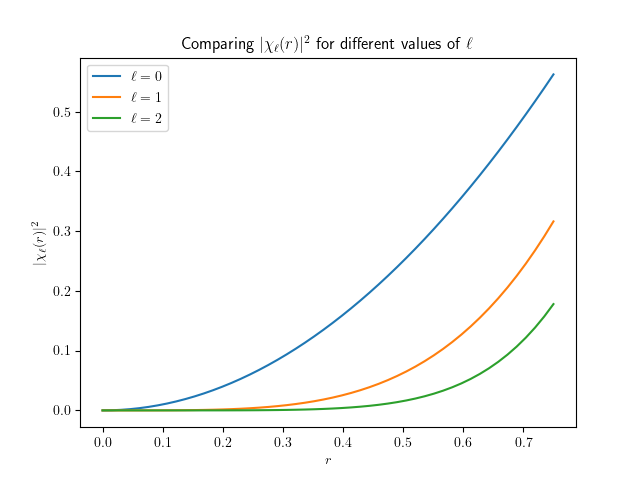
\includegraphics[scale=0.6]{chi_l_squared.png}
    \caption{\(\abs{\chi_\ell(r)}^2\) compared for \(\ell = 0, 1, 2\) and \(r < 1\).}
    \label{fig:chi for low r}
\end{figure}
Figure~\ref{fig:chi for low r} shows \(\abs{\chi_\ell(r)}^2\) plotted for \(\ell = 0, 1, 2\).
We see that the larger the value of \(\ell\) the less likely the particle is to be near the origin.
This can be see as analogous to the classical centrifugal potential which provides a force away from the origin.
In quantum mechanics a centrifugal term in the potential instead decreases the probability of the particle being near the origin.

There are two probabilities that we may be interested in.
The \gls{pdf} for finding the particle at a specific point, \(\vv{r}\) is \(\abs{u(r, \vartheta, \varphi)}^2\) so the probability that the particle is in the volume \(\dd{V}\) is \(\abs{u(r, \vartheta, \varphi)}^2\dd{V}\).
The probability that the particle is in a given volume, \(V\), is then
\[\int_V \abs{u(r, \vartheta, \varphi)}^2.\]
The \gls{pdf} for finding the particle at some specific radius, \(\vv{r}\) is \(\abs{\chi_\ell(r)}^2\) so the probability that the particle is at a point with radius \([r, r + \dd{r}]\) is
\[\int\dd{\Omega}\abs{u(r, \vartheta, \varphi)}^2 = \int\dd{\Omega}\abs{Y_\ell^m(\vartheta, \varphi)}^2\abs{\chi_\ell(r)}^2\dd{r} = \abs{\chi_\ell(r)}^2\dd{r}.\]
The probability that the particle is at some point with a radius in \([a, b]\) is then
\[\int_a^b\dd{r}\abs{\chi_\ell(r)}^2.\]

\section{Spin}
We saw in section~\ref{sec:Bounds on m} that the angular momentum quantum number, \(\ell\), is always an integer despite the fact that the similarly defined \(j\) can take half integer values.
This is because of the spatial dependence of the solutions.
For the eigenfunctions of \(\operator{L}^2\) to be single valued we require that
\[Y_\ell^m(\vartheta, \varphi) = Y_\ell^m(\vartheta, \varphi + 2\pi)\]
and we saw that the \(\varphi\) dependence of \(Y_\ell^m\) was
\[Y_\ell^m(\vartheta, \varphi) \propto e^{im\varphi}.\]
In combination these two equations mean that \(m\) must be an integer.
Since \(m\) takes on any value from \(-\ell\) to \(\ell\) this means that \(\ell\) must be an integer.

\define{Spin} is an intrinsic property of a quantum system.
It is like angular momentum in that the spin is associated with the operator
\[\vecoperator{S} = (\operator{S}_1, \operator{S}_2, \operator{S}_3),\]
with the commutation relation
\[[\operator{S}_k, \operator{S}_l] = i\hbar\varepsilon_{klm}\operator{S}_m.\]
This was the assumption that we made at the start of section~\ref{sec:algebraic solution to the eigenvalue problem} so we can use everything we derived in that section.
In particular we can define 
\[\operator{S}^2 = \operator{S}_x^2 + \operator{S}_y^2 + \operator{S}_z^2.\]
\(\operator{S}^2\) and \(\operator{S}_z\) are a \gls{csco} and have a common eigenbasis:
\[\left\{\ket{s, m}\st m = -s, 1 - s, \dotsc, s - 1, s~\text{and}~s = \frac{n}{2}~\text{where}~n\in\naturals\right\}.\]
The action of \(\operator{S}^2\) and \(\operator{S}_z\) on these basis vectors is
\[\operator{S}^2\ket{s, m} = s(s + 1)\hbar^2\ket{s, m}, \qquad\text{and}\qquad \operator{S}_z\ket{s, m} = m\hbar\ket{s, m}.\]
For a fixed value of \(s\) we see that this is a \((2s + 1)\)-state system.

From now on we focus only on spin 1/2 systems.
That is systems where \(s = 1/2\).
This includes electrons, protons, neutrons, neutrinos, and quarks.
So most matter that we come across day to day.
In this case we have a two dimensional vector space, \(\hilbert_{\text{spin}}\), with a basis
\[\left\{\ket{\tfrac{1}{2}, \tfrac{1}{2}}, \ket{\tfrac{1}{2}, -\tfrac{1}{2}}\right\}.\]
Since \(s = 1/2\) for both of these it is common to introduce a shorter notation where we refer to \(\ket{\tfrac{1}{2}, \tfrac{1}{2}}\) as spin up, denoted \(\ket{\tfrac{1}{2}}\) or \(\ket{\spinUp}\), and \(\ket{\tfrac{1}{2}, -\tfrac{1}{2}}\) as spin down, denoted \(\ket{-\tfrac{1}{2}}\) or \(\ket{\spinDown}\).
These are still eigenfunctions of both \(\operator{S}^2\) and \(\operator{S}_z\):
\[\operator{S}^2\ket{\spinUp} = \frac{3}{4}\hbar^2\ket{\spinUp}, \qquad, \operator{S}^2\ket{\spinDown} = \frac{3}{4}\hbar^2\ket{\spinDown},\]
\[\operator{S}_z\ket{\spinUp} = \frac{\hbar}{2}, \qquad\text{and}\qquad \operator{S}_z\ket{\spinDown} = -\frac{\hbar}{2}\ket{\spinDown}.\]
A generic spin state, \(\ket{\psi}\in\hilbert_\text{spin}\) is given by
\[\ket{\psi} = \psi_1\ket{\spinUp} + \psi_2\ket{\spinDown}\]
where as usual \(\psi_1 = \braket{\spinUp}{\psi}\), \(\psi_2 = \braket{\spinDown}{\psi}\), and \(\abs{\psi_1}^2 + \abs{\psi_2}^2 = 1\).
Since spin has no spatial dependence we describe spin with vectors in \(\hilbert_\text{spin}\).
If a system also has spatial dependence then we can describe this with vectors in some other vector space \(\hilbert_\text{space}\).
The full description of a state is then given by a vector in
\[\hilbert = \hilbert_\text{space}\tensorProd\hilbert_\text{spin}.\]
\(\hilbert\) has as a basis
\[\left\{ \ket{\vv{r}, m}\st \vv{r}\in\reals^3 ~\text{and}~ m = \pm\frac{1}{2} \right\}.\]
The vectors in this basis are simply the tensor products of vectors of the individual bases of \(\hilbert_\text{space}\) and \(\hilbert_\text{spin}\):
\[\ket{\vv{r}, m} = \ket{\vv{r}}\ket{m} = \ket{\vv{r}}\tensorProd\ket{m}.\]
This basis is complete, meaning
\[\int \dd[3]{r'} \sum_{m} \ketbra{\vv{r'}, m}{\vv{r'}, m} = \ident.\]
A generic state, \(\ket{\psi}\in\hilbert\), is then given by
\begin{align*}
    \ket{\psi} &= \int\dd[3]{r} \sum_m \ket{\vv{r'}, m}\braket{\vv{r'}, m}{\psi}\\
    &= \int\dd[3]{r'}\sum_m \psi_m(\vv{r'})\ket{\vv{r'}, m}\\
    &= \int\dd[3]{r'}\left[\psi_1(\vv{r'})\ket{\spinUp} + \psi_2(\vv{r'})\ket{\spinDown}\right]
\end{align*}
where \(\psi_m(\vv{r'}) = \braket{\vv{r'}, m}{\psi}\).
Taking the inner product with a position eigenstate, \(\ket{\vv{r}}\), we have
\begin{align*}
    \braket{\vv{r}}{\psi} &= \int \dd[3]{r'}\sum_m \braket{\vv{r}}{\vv{r'}}\ket{m}\psi_m(\vv{r'})\\
    &= \int \dd[3]{r'} \sum_m \delta(\vv{r} - \vv{r'})\ket{m}\psi_m(\vv{r'})\\
    &= \sum_m \int \dd[3]{r'} \delta(\vv{r} - \vv{r'})\ket{m}\psi_m(\vv{r'})\\
    &= \sum_m \psi_m(\vv{r})\\
    &= \psi_1(\vv{r})\ket{\spinUp} + \psi_2(\vv{r})\ket{\spinDown}.
\end{align*}
In the basis \(\{\ket{\spinUp}, \ket{\spinDown}\}\) for \(\hilbert_\text{spin}\) we can denote \(\braket{\vv{r}}{\psi}\) as a column vector:
\[
\braket{\vv{r}}{\psi} \representation 
\begin{pmatrix}
    \psi_1(\vv{r})\\ \psi_2(\vv{r})
\end{pmatrix}
.
\]
The interpretation of these values is as follows:
\begin{itemize}
    \item \(\abs{\psi_1(\vv{r})^2}\) -- the \gls{pdf} of finding the system at \(\vv{r}\) with spin up.
    \item \(\abs{\psi_2(\vv{r})^2}\) -- the \gls{pdf} of finding the system at \(\vv{r}\) with spin down.
    \item The probability of finding the system anywhere in space with spin up is
    \[P(\spinUp) = \int\dd[3]{r}\abs{\psi_1(\vv{r})}^2.\]
    \item The probability of finding the system anywhere in space with spin down is
    \[P(\spinDown) = \int\dd[3]{r}\abs{\psi_2(\vv{r})}^2.\]
    \item The probability of finding the system at \(\vv{r}\) with any spin is
    \[P(\vv{r}) = \abs{\psi_1(\vv{r})}^2 + \abs{\psi_2(\vv{r})}^2.\] 
\end{itemize}

\subsection{Matrix Elements}
\(\hilbert_{\text{spin}}\) is a two-dimensional vector space.
Therefore the spin operators can be represented by \(2\times 2\) matrices acting on column vectors.
First we start with
\[\operator{S}_z\ket{\spinUp} = \frac{\hbar}{2}\ket{\spinUp}, \qquad\text{and}\qquad \operator{S}_z\ket{\spinDown} = -\frac{\hbar}{2}\ket{\spinDown}.\]
Hence
\begin{align*}
    \bra{\spinUp}\operator{S}_z\ket{\spinUp} &= \frac{\hbar}{2},\\
    \bra{\spinUp}\operator{S}_z\ket{\spinDown} &= 0,\\
    \bra{\spinDown}\operator{S}_z\ket{\spinUp} &= 0,
    \shortintertext{and}
    \bra{\spinDown}\operator{S}_z\ket{\spinDown} &= -\frac{\hbar}{2}.
\end{align*}
This can be written compactly as
\[\bra{m'}\operator{S}_z\ket{m} = \sign(m)\delta_{m'm}\frac{\hbar}{2}.\]
Thus in this basis \(\operator{S}_z\) is represented by
\[
\operator{S}_z \representation \frac{\hbar}{2}
\begin{pmatrix}
    1 & 0\\
    0 & -1
\end{pmatrix}
.
\]
Where we follow the convention that the first row (column) corresponds to the largest value of \(m'\) (\(m\)) so that the first row (column) is labelled by \(m' = 1/2\) (\(m = 1/2\)) and the second row (column) is labelled by \(m' = -1/2\) (\(m = -1/2\)).

As before we define the operators
\[\operator{S}_+ = \operator{S}_x + i\operator{S}_y, \qquad\text{and}\qquad \operator{S}_- = \operator{S}_x - i\operator{S}_y.\]
These have the expected action that
\[\operator{S}_+\ket{\spinUp} = 0, \qquad \operator{S}_+\ket{\spinDown} = \hbar c_+\ket{\spinUp} = \hbar \sqrt{\frac{1}{2}\left(\frac{1}{2} + 1\right) + \frac{1}{2}\left(-\frac{1}{2} + 1\right)}\ket{\spinUp} = \hbar\ket{\spinUp}\]
\[\operator{S}_-\ket{\spinDown} = 0, \qquad\text{and}\qquad \operator{S}_-\ket{\spinUp} = \hbar c_-\ket{\spinDown} = \hbar\sqrt{\frac{1}{2}\left(\frac{1}{2} + 1\right) - \frac{1}{2}\left(\frac{1}{2} + 1\right)} = \hbar\ket{\spinDown}.\]
Hence
\begin{align*}
    \bra{\spinUp}\operator{S}_+\ket{\spinUp} = 0, \qquad & \bra{\spinUp}\operator{S}_-\ket{\spinUp} = 0,\\
    \bra{\spinUp}\operator{S}_+\ket{\spinDown} = \hbar, \qquad & \bra{\spinUp}\operator{S}_-\ket{\spinDown} = 0,\\
    \bra{\spinDown}\operator{S}_+\ket{\spinUp} = 0, \qquad & \bra{\spinDown}\operator{S}_-\ket{\spinUp} = \hbar,\\
    \bra{\spinDown}\operator{S}_+\ket{\spinDown} = 0, \qquad & \bra{\spinDown}\operator{S}_-\ket{\spinDown} = 0.
\end{align*}
Thus in this basis these operators are represented by
\[
\operator{S}_+ \representation\hbar
\begin{pmatrix}
    0 & 1\\
    0 & 0
\end{pmatrix}
\qquad\text{and}\qquad
\operator{S}_- \representation\hbar
\begin{pmatrix}
    0 & 0\\
    1 & 0
\end{pmatrix}
.
\]
Now we can write
\[\operator{S}_x = \frac{1}{2}\left(\operator{S}_+ + \operator{S_-}\right), \qquad\text{and}\qquad \operator{S}_y = \frac{1}{2i}\left(\operator{S}_+ - \operator{S}_-\right).\]
Thus the representations of \(\operator{S}_x\) and \(\operator{S}_y\) in this basis are
\[
\operator{S}_x \representation \frac{\hbar}{2}
\begin{pmatrix}
    0 & 1\\
    1 & 0
\end{pmatrix}
\qquad\text{and}\qquad
\operator{S}_y \representation \frac{\hbar}{2}
\begin{pmatrix}
    0 & -i\\
    i & 0
\end{pmatrix}
.
\]
The three matrices representing \(\operator{S}_k\) in this basis are called the \define{Pauli spin matrices}:
\[
\sigma_x =
\begin{pmatrix}
    0 & 1\\
    1 & 0
\end{pmatrix}
,\qquad \sigma_y =
\begin{pmatrix}
    0 & -i\\
    i & 0
\end{pmatrix}
,\qquad\text{and}\qquad \sigma_z = 
\begin{pmatrix}
    1 & 0\\
    0 & 1
\end{pmatrix}
.
\]
Which allows us to compactly write
\[\operator{S}_k \representation \frac{\hbar}{2}\sigma_k, \qquad\text{and}\qquad \vecoperator{S} = \frac{\hbar}{2}\vv{\sigma}\]
where \(\vv{\sigma} = (\sigma_x, \sigma_y, \sigma_z)\).
The Pauli matrices are Hermitian, as they are associated with observables, and also unitary, meaning \(\sigma_k\sigma_k\hermit = \sigma_k^2 = \ident\), they also all have zero trace, \(\tr(\sigma_k) = 0\).
We can then use \(\sigma\) as another label for the basis vectors, for example if we define
\[\ket{\psi} = \sum_{\sigma} \psi_\sigma\ket{\sigma}\]
then we can characterise the action of \(\operator{S}_k\) as
\[\ket{\varphi} = \operator{S}_k = \sum_\sigma \varphi_\sigma\ket{\sigma} = \sum_\sigma\sum_{\sigma'}(S_k)_{\sigma\sigma'}\psi_{\sigma'}\ket{\sigma}\]
where we have used
\[\varphi_\sigma = \sum_{\sigma'}(S_k)_{\sigma\sigma'}\psi_{\sigma'}.\]

We can now use the definition of \(\operator{S}^2\) to find a representation for \(\operator{S}^2\) in this basis:
\begin{align*}
    \operator{S}^2 &= \sum_k \operator{S}_k^2\\
    &\representation \sum_k \left(\frac{\hbar}{2}\sigma_k\right)^2\\
    &= \sum_k \frac{\hbar^2}{4}\sigma_k^2\\
    &= \sum_k \frac{\hbar^2}{4}\ident\\
    &= \frac{3}{4}\hbar^2\ident\\
    &= \frac{3}{4}\hbar^2
    \begin{pmatrix}
        1 & 0\\
        0 & 1
    \end{pmatrix}
\end{align*}

\subsection{Eigenvectors of \texorpdfstring{\(\operator{S}_z\)}{Sz} and \texorpdfstring{\(\operator{S}^2\)}{S2}}
The eigenvectors of \(\sigma_z\) are easy to find:
\[
\begin{pmatrix}
    1 & 0\\
    0 & -1
\end{pmatrix}
\begin{pmatrix}
    1\\ 0
\end{pmatrix}
=
\begin{pmatrix}
    1\\ 0
\end{pmatrix}
,\qquad\text{and}\qquad
\begin{pmatrix}
    1 & 0\\
    0 & -1
\end{pmatrix}
\begin{pmatrix}
    0\\ 1
\end{pmatrix}
= -
\begin{pmatrix}
    0\\ 1
\end{pmatrix}
.
\]
So the eigenvalues of this representation of \(\operator{S}_z\) are given by
\[
\frac{\hbar}{2}
\begin{pmatrix}
    1 & 0\\
    0 & -1
\end{pmatrix}
\begin{pmatrix}
    1\\ 0
\end{pmatrix}
= \frac{\hbar}{2}
\begin{pmatrix}
    1\\ 0
\end{pmatrix}
,\qquad\text{and}\qquad
\frac{\hbar}{2}
\begin{pmatrix}
    1 & 0\\
    0 & -1
\end{pmatrix}
\begin{pmatrix}
    0\\ 1
\end{pmatrix}
= -\frac{\hbar}{2}
\begin{pmatrix}
    0\\ 1
\end{pmatrix}
.
\]
We see that these have the eigenvalues \(\pm\hbar/2\), which is what we would expect for a spin 1/2 system.
These eigenvectors are also simultaneously eigenvectors of \(\operator{S}^2\) in this representation, this is trivial since \(\operator{S}^2\) is proportional to the identity in this representation:
\[
\frac{3}{4}\hbar^2
\begin{pmatrix}
    1 & 0\\
    0 & 1
\end{pmatrix}
\begin{pmatrix}
    1\\ 0
\end{pmatrix}
= \frac{3}{4}\hbar^2
\begin{pmatrix}
    1\\ 0
\end{pmatrix}
,\qquad\text{and}\qquad
\frac{3}{4}\hbar^2
\begin{pmatrix}
    1 & 0\\
    0 & 1
\end{pmatrix}
\begin{pmatrix}
    0\\ 1
\end{pmatrix}
= \frac{3}{4}\hbar^2
\begin{pmatrix}
    0\\ 1
\end{pmatrix}
.
\]
Thus we can identify
\[
\ket{s=\tfrac{1}{2}, m=\tfrac{1}{2}} = \ket{\spinUp} \representation 
\begin{pmatrix}
    0\\ 1
\end{pmatrix}
,\qquad\text{and}\qquad
\ket{s = \tfrac{1}{2}, m=-\tfrac{1}{2}} = \ket{\spinDown} \representation
\begin{pmatrix}
    1\\ 0
\end{pmatrix}
.
\]
A generic vector, \(\ket{\psi}\in\hilbert_{\text{spin}}\), can then be represented by
\[
\ket{\psi} = \psi_1\ket{\spinUp} + \psi_2\ket{\spinDown} \representation
\begin{pmatrix}
    \psi_1\\
    \psi_2
\end{pmatrix}
=
\psi_1
\begin{pmatrix}
    1\\ 0
\end{pmatrix}
+ \psi_2
\begin{pmatrix}
    0\\ 1
\end{pmatrix}
.
\]
Note that in general \(\psi_k\in\complex\) so the space spanned by these eigenvectors is not \(\reals^2\) but \(\complex^2\).

\subsection{Scalar Products}
Now that we have representations of generic vectors in this basis we ask what is the representation of a covector, \(\bra{\psi}\in\hilbert_{\text{spin}}^*\)?
The answer, as always, is that if \(\ket{\psi}\) is represented by an \(n\)-dimensional column vector then \(\bra{\psi}\) is represented by an \(n\)-dimensional row vector with the components given by
\[
\ket{\psi} \representation 
\begin{pmatrix}
    \psi_1\\ \psi_2
\end{pmatrix}
\implies
\bra{\psi} \representation
\begin{pmatrix}
    \psi_1^* & \psi_2^*
\end{pmatrix}
.
\]
That is \(\bra{\psi} = (\ket{\psi})\hermit\).
The scalar product of two states, \(\ket{\psi}\) and \(\ket{\varphi}\), is then
\[
\braket{\varphi}{\psi} =
\begin{pmatrix}
    \varphi_1^* & \varphi_2^*
\end{pmatrix}
\begin{pmatrix}
    \psi_1\\ \psi_2
\end{pmatrix}
= \varphi_1^*\psi_1 + \varphi_2^*\psi_2.
\]
For example if \(\ket{\psi}\) is a properly normalised state then
\[
\braket{\varphi}{\psi} =
\begin{pmatrix}
    \psi_1^* & \psi_2^*
\end{pmatrix}
\begin{pmatrix}
    \psi_1\\ \psi_2
\end{pmatrix}
= \abs{\psi_1}^2 + \abs{\varphi_2}^2  = 1.
\]

\subsection{Spin Along the \texorpdfstring{\(x\)}{x} Direction}
We can find the possible values of \(m_x\) by finding the eigenvalues of \(\hbar\sigma_x/2\) in the \(\operator{S}_z\) eigenbasis.
We do this in the normal way:
\begin{align*}
    0 &= \det\left(\frac{\hbar}{2}\sigma_x - \lambda\ident\right)\\
    &= 
    \begin{vmatrix}
        -\lambda & \hbar/2\\
        \hbar/2 & -\lambda
    \end{vmatrix}
    \\
    &= \lambda^2 - \frac{\hbar^2}{4}
\end{align*}
So \(S_x = \lambda = \pm \hbar/2\).
This is the same as the possible values of \(S_z\), this is what we would expect from the symmetry of the situation, there is nothing important about the \(z\) or \(x\) directions that would mean they have different possible values of \(S_k\).
We can write a state with \(m_x = 1/2\) as a combination of the basis vectors:
\[\ket{m_x = 1/2} = \alpha\ket{\spinUp} + \beta\ket{\spinDown}.\]
In this representation this becomes
\[
\operator{S}_x\ket{m_x = 1/2} = \frac{\hbar}{2}\ket{m_x = 1/2} \representation \frac{\hbar}{2}\sigma_x
\begin{pmatrix}
    \alpha\\ \beta
\end{pmatrix}
=
\frac{\hbar}{2}
\begin{pmatrix}
    0 & 1\\
    1 & 0
\end{pmatrix}
\begin{pmatrix}
    \alpha\\ \beta
\end{pmatrix}
= \frac{\hbar}{2}
\begin{pmatrix}
    \beta\\ \alpha
\end{pmatrix}
= \frac{\hbar}{2}
\begin{pmatrix}
    \alpha\\ \beta
\end{pmatrix}
.
\]
Hence \(\alpha = \beta\) so a properly normalised state with \(m_x = \hbar/2\) is
\[\ket{m_x = 1/2} = \frac{\sqrt{2}}{2}\left[\ket{\spinUp} + \ket{\spinDown}\right].\]
We can show in a similar way that if \(S_x = -1/2\) then
\[\ket{m_x = -1/2} = \frac{\sqrt{2}}{2}\left[\ket{\spinUp} - \ket{\spinDown}\right].\]

It can be shown that if we measure the spin along any vector in the \((x, z)\)-plane at an angle \(\vartheta\) to the \(z\) axis,
\[\vh{n} = \sin(\vartheta)\ve{x} + \cos(\vartheta)\ve{z},\]
then the relevant eigenstates in the the representation that we are using are the eigenvalues of
\[
\vv{\sigma}\cdot\vh{n} = \sigma_x\sin(\vartheta) + \sigma_z\cos(\vartheta) = 
\begin{pmatrix}
    \cos\vartheta & \sin\vartheta\\
    \sin\vartheta & -\cos\vartheta
\end{pmatrix}
.
\]

\section{Addition of Angular Momenta}\label{sec:addition of angular momenta}
Suppose we have two systems with independent angular momenta \(\vecoperator{J}^{(1)}\) and \(\vecoperator{J}^{(2)}\).
This could be two particles with angular momentum, two particles with spin or one particle with angular momentum and spin.
These operators satisfy the usual commutation relations,
\[\left[\operator{J}^{(n)}_k, \operator{J}^{(n)}_l\right] = i\hbar\varepsilon_{klm}\operator{J}^{(n)}_m, \qquad\text{and}\qquad \left[\angmomsquared{n}, \operator{J}^{(n)}_k\right] = 0.\]
Since the two angular momenta are independent the operators associated with different angular momenta commute:
\[\left[\operator{J}^{(1)}_k, \operator{J}^{(2)}_l\right] = \left[\angmomsquared{1}, \angmomsquared{2}\right] = \left[\angmomsquared{1}, \operator{J}^{(2)}_k\right] = 0 \qquad\text{etc.}\]
We can extend this easily to any number of independent angular momenta but we won't here.

\subsection{Vector Spaces}
Since \(\vecoperator{J}^{(1)}\) and \(\vecoperator{J}^{(2)}\) commute they form a \gls{csco} which means we can find a common eigenbasis.
Since both angular momenta are independent we can describe both with separate Hilbert spaces.
Angular momentum 1 is described by vectors in a vector space \(\hilbert^{(1)}\).
For a particular value, \(j^{(1)}\), of the angular momentum quantum number this is a \(2j_1 + 1\) dimensional vector space.
This space has as a basis \(\{\ket{j_1, m_1}\}\)
Similarly angular momentum 2 is described by vectors in the \(2j_2 + 1\) dimensional vector space, \(\hilbert^{(2)}\), with basis \(\ket{j_2, m_2}\).
The entire system is then described by vectors in
\[\hilbert = \hilbert^{(1)}\tensorProd\hilbert^{(2)}.\]
The dimensionality of this vector space is
\[\dim(\hilbert) = \dim(\hilbert^{(1)})\dim(\hilbert^{(2)}) = (2j_1 + 1)(2j_2 + 1).\]
This space then has as a basis
\[\{\ket{j_1, m_1, j_2, m_2}\} = \{\ket{j_1, m_1}\tensorProd\ket{j_2, m_2}\}.\]
As usual we extend the definition of the operators so that they act on only their respective parts of these vectors.
Strictly we should define new operators like \({\operator{J}^{(1)}_z}{'} = \operator{J}^{(1)}_z\tensorProd\ident\) which then acts on \(\ket{j_1, m_1, j_2, m_2} = \ket{j_1, m_1}\tensorProd\ket{j_2, m_2}\) as
\begin{align*}
    {\operator{J}^{(1)}_z}{'}\ket{j_1, m_1, j_2, m_2} &= (\operator{J}^{(1)}_z\tensorProd\ident)(\ket{j_1, m_1}\tensorProd\ket{j_2, m_2})\\
    &= \operator{J}^{(1)}_z\ket{j_1, m_1}\tensorProd\ident\ket{j_2, m_2}\\
    &= \hbar m_1\ket{j_1, m_1}\tensorProd\ket{j_2, m_2}\\
    &= \hbar m_1\ket{j_1, m_1, j_2, m_2}
\end{align*}
but in practice we use the same symbol for both operators, \(\operator{J}^{(1)}_z\colon\hilbert^{(1)}\to\complex\) and \(\operator{J}^{(1)}_z{'}\colon\hilbert\to\complex\).
The action of the operators on this basis is
\begin{align*}
    \angmomsquared{1}\ket{j_1, m_1, j_2, m_2} &= \hbar^2j_1(j_1 + 1)\ket{j_1, m_1, j_2, m_2},\\
    \operator{J}^{(1)}_z\ket{j_1, m_1, j_2, m_2} &= \hbar m_1\ket{j_1, m_1, j_2, m_2},\\
    \angmomsquared{2}\ket{j_1, m_1, j_2, m_2} &= \hbar^2j_2(j_2 + 1)\ket{j_1, m_1, j_2, m_2},\\
    \operator{J}^{(2)}_z\ket{j_1, m_1, j_2, m_2} &= \hbar m_2\ket{j_1, m_1, j_2, m_2}.
\end{align*}
A generic state, \(\ket{\psi}\in\hilbert\), can be given as
\[\ket{\psi} = \sum_{j_1, m_2, j_2, m_2} c_{j_1m_1j_2m_2}\ket{j_1, m_1, j_2, m_2}\]
where
\[c_{j_1m_1j_2m_2} = \braket{j_1, m_1, j_2, m_2}{\psi}.\]

\subsection{Total Angular Momentum}\label{sec:total angular momentum}
We can now define the total angular momentum:
\[\vecoperator{J} = \vecoperator{J}^{(1)} + \vecoperator{J}^{(2)}.\]
This satisfies the normal angular momentum commutation relations:
\[[\operator{J}_k, \operator{J}_l] = i\hbar\varepsilon_{klm}\operator{J}_m, \qquad\text{and}\qquad [\operator{J}^2, \operator{J}_k] = 0.\]
This means that \(\operator{J}^2\) and \(\operator{J}_z\) form a \gls{csco} so we can find a simultaneous eigenbasis for \(\hilbert\) made of vectors of the form \(\{\ket{j, m}\}\).
What values can \(j\) and \(m\) take?
The answer lies in the angular momentum addition theorem, which we won't prove here:
\begin{theorem}{Angular momentum addition theorem}{}
    Given two independent angular momenta with corresponding quantum numbers, \(j_1\) and \(j_2\), the allowed value of the angular momentum quantum number for the total angular momentum are
    \[j = j_1 + j_2, j_1 + j_2 - 1, \dotsc, \abs{j_1 - j_2}.\]
    For each of these values we also have
    \[m = -j, -j + 1, \dotsc, j - 1, j.\]
\end{theorem}
Before we said that \(\dim(\hilbert) = (2j_1 + 1)(2j_2 + 1)\).
We can check that this is consistent with the angular momentum addition theorem.
Without loss of generality assume that \(j_1 \ge j_2\).
Then
\begin{align*}
    \dim(\hilbert) &= \sum_{\mathclap{j=j_1 - j_2}}^{\mathclap{j_1 + j_2}} (2j + 1)\\
    &= \sum_{j=0}^{\mathclap{j_1 + j_2}} (2j + 1) - \sum_{j = 0}^{\mathclap{j_1 - j_2 - 1}} (2j + 1)\\
    &= 2\sum_{j=0}^{\mathclap{j_1 + j_2}} j + (j_1 + j_2) - 2\sum_{j = 0}^{\mathclap{j_1 - j_2 - 1}} j - (j_1 - j_2 - 1 )\\
    &= (j_1 + j_2)(j_1 + j_2 + 1) + (j_1 + j_2) - (j_1 - j_2 - 1)(j_1 - j_2) - (j_1 - j_2 - 1)\\
    &= j_1^2 + j_2^2 + 2j_1j_2 + j_1 + j_2 + j_1 + j_2 - j_1^2 - j_2^2 + 2j_1j_2 + j_1 - j_2 - j_1 + j_2 + 1\\
    &= 4j_1j_2 + 2j_1 + 2j_2 + 1\\
    &= (2j_1 + 1)(2j_2 + 1).\\
\end{align*}
Where we have used
\[\sum_{r = 0}^n = \frac{1}{2}n(n + 1),\]
which is proven in appendix~\ref{sec:proof sum 0 to n of r is 0.5 n(n+1)}.
Both bases, \(\{\ket{j_1, m_1, j_2, m_2}\}\) and \(\{\ket{j, m}\}\), are orthonormal so there exists a unitary transformation between the two bases.
For fixed \(j_1\) and \(j_2\) we denote \(\ket{j, m}\) as \(\ket{j, m; j_1, j_2}\) to denote the specific values that \(j_1\) and \(j_2\) are held at.
Using the completeness of the \(\{\ket{j_1, m_1, j_2, m_2}\}\) basis,
\[\sum_{m_1, m_2} \braket{j_1, m_1, j_2, m_2}{j_1, m_1, j_2, m_2} = \ident\]
we have
\[\ket{j, m; j_1, j_2} = \sum_{m_1, m_2} \ket{j_1, m_1, j_2, m_2}\braket{j_1, m_1, j_2, m_2}{j, m; j_1, j_2}.\]
The quantities \(\braket{j_1, m_1, j_2, m_2}{j, m; j_1, j_2}\) are called the Clebsch--Gordan coefficients and they are tabulated in many sources.

The basis \(\{\ket{j_1, m_1, j_2, m_2}\}\) is called the \define{uncoupled basis} as vectors in this basis can be written as two parts, one related to angular momentum 1 and the other related to angular momentum 2, for example a basis vector can be written as \(\ket{j_1, m_1}\tensorProd\ket{j_2, m_2}\) and a generic vector as
\[\ket{\psi} = \sum_{\mathclap{j_1, m_1, j_2, m_2}}(\braket{j_1, m_1}{\psi}\ket{j_1, m_1} \tensorProd\braket{j_2, m_2}{\psi}\ket{j_2, m_2}).\]
The basis \(\{\ket{j, m}\}\) is called the \define{coupled basis} as this is not possible.

\begin{example}
    Consider a system composed of two spin 1/2 particles.
    \(\hilbert^{(1)}\) is a two dimensional vector space with a basis
    \[\{s_1, m_1\} = \{\ket{\tfrac{1}{2}, \tfrac{1}{2}}, \ket{\tfrac{1}{2}, -\tfrac{1}{2}}\}.\]
    \(\hilbert^{(2)}\) is also a two dimensional vector space with basis
    \[\{s_2, m_2\} = \{\ket{\tfrac{1}{2}, \tfrac{1}{2}}, \ket{\tfrac{1}{2}, -\tfrac{1}{2}}\}.\]
    The spin of the whole system is then characterised by vectors in \(\hilbert = \hilbert^{(1)}\tensorProd\hilbert^{(2)}\) which has the basis
    \[\{\ket{s_1, m_1, s_2, m_2}\} = \{\ket{\tfrac{1}{2},\tfrac{1}{2},\tfrac{1}{2},\tfrac{1}{2}}, \ket{\tfrac{1}{2},\tfrac{1}{2},\tfrac{1}{2},-\tfrac{1}{2}}, \ket{\tfrac{1}{2},-\tfrac{1}{2},\tfrac{1}{2},\tfrac{1}{2}}, \ket{\tfrac{1}{2},-\tfrac{1}{2},\tfrac{1}{2},-\tfrac{1}{2}}\}.\]
    Since \(s_i = 1/2\) for all states in this system we compactly write this basis as
    \[\{\ket{\spinUp\spinUp}, \ket{\spinUp\spinDown}, \ket{\spinDown\spinUp}, \ket{\spinDown, \spinDown}\}.\]
    Where the first arrow denotes particle 1's spin and the second arrow denotes particle 2's spin.
    The values that \(s\) can take, as given by the angular momentum addition theorem, is \(s = s_1 + s_2, \abs{s_1 - s_2} = 1, 0\).
    So the entire system has spin 1 or spin 0.
    To find the uncoupled basis consider the action of \(\operator{S}_z\) on the coupled basis
    \[\operator{S}_z\ket{\spinUp\spinUp} = (\operator{S}^{(1)}_z + \operator{S}^{(2)}_z)\ket{\spinUp\spinUp} = \frac{\hbar}{2}\ket{\spinUp\spinUp} + \frac{\hbar}{2}\ket{\spinUp\spinUp} = \hbar\ket{\spinUp\spinUp}.\]
    Hence \(m = 1\).
    Since \(m > 0\) we know that \(s \ne 0\) so \(s = 1\).
    Similarly
    \[\operator{S}_z\ket{\spinDown\spinDown} = (\operator{S}^{(1)}_z + \operator{S}^{(2)}_z)\ket{\spinDown\spinDown} = -\frac{\hbar}{2}\ket{\spinDown\spinDown} + -\frac{\hbar}{2}\ket{\spinDown\spinDown} = -\hbar\ket{\spinDown\spinDown}.\]
    Hence \(m = 1\) and \(s = 1\) for this state.
    So far we have
    \[\ket{1,1} = \ket{\spinUp\spinUp}, \qquad\text{and}\qquad \ket{1,-1} = \ket{\spinDown\spinDown}.\]
    We don't yet know what \(\ket{1, 0}\) or \(\ket{0, 0}\) are.
    The difficulty in finding these states is that they aren't uniquely identified purely by the value of \(m\).
    However we do know how to construct them from other states using raising and lowering operators.
    The lowering operator for the total angular momentum is simply
    \[\operator{S}_- = \operator{S}^{(1)}_- + \operator{S}^{(2)}_-\]
    so by identifying that we expect
    \[\operator{S}_-\ket{1, 1} \propto \ket{1, 0}\]
    we know that
    \[\ket{1, 0} \propto \operator{S}_-\ket{\spinUp\spinUp} = (\operator{S}^{(1)}_- + \operator{S}^{(2)}_-)\ket{\spinUp\spinUp} = \operator{S}^{(1)}_-\ket{\spinUp\spinUp} + \operator{S}^{(2)}_-\ket{\spinUp\spinUp} \propto \ket{\spinDown\spinUp} + \ket{\spinUp\spinDown}.\]
    Using the fact that the uncoupled basis vectors are orthonormal we have
    \[\ket{1, 0} = \frac{\sqrt{2}}{2}(\ket{\spinUp\spinDown} + \ket{\spinUp\spinDown}).\]
    Finally \(\ket{0, 0}\) must be a linear combination of \(\ket{\spinUp\spinDown}\) and \(\ket{\spinDown\spinUp}\) and it must be orthogonal to \(\ket{1, 0}\).
    We are then free to chose that
    \[\ket{0, 0} = \frac{\sqrt{2}}{2}(\ket{\spinUp\spinDown} - \ket{\spinDown\spinUp}).\]
    This agrees with the Clebsch--Gordan coefficients which are tabulated in table~\ref{tab:clebsch-gordan coefficients j = 1}.
    \begin{table}[ht]
        \centering
        \begin{subtable}{0.25\textwidth}
            \centering
            \begin{tabular}{|l|l|}\hline
                \backslashbox{\(m_1, m_2\)}{\(j\)} & 1\\ \hline
                \(1/2, 1/2\) & 1\\ \hline
            \end{tabular}
            \subcaption{\(m = 1\)}
        \end{subtable}
        \begin{subtable}{0.25\textwidth}
            \centering
            \begin{tabular}{|l|l|}\hline
                \backslashbox{\(m_1, m_2\)}{\(j\)} & 1\\ \hline
                \(-1/2, -1/2\) & 1\\ \hline
            \end{tabular}
            \subcaption{\(m = -1\)}
        \end{subtable}
        \begin{subtable}{0.4\textwidth}
            \centering
            \begin{tabular}{|l|l|l|}\hline
                \backslashbox{\(m_1, m_2\)}{\(j\)} & 1 & 0\\ \hline
                \(1/2, -1/2\) & \(\sqrt{2}/2\) & \(\sqrt{2}/2\)\\ \hline
                \(-1/2, 1/2\) & \(\sqrt{2}/2\) & -\(\sqrt{2}/2\)\\ \hline
            \end{tabular}
            \subcaption{\(m = 0\)}
        \end{subtable}
        
        
        \caption{Clebsch--Gordan coefficients for two spin 1/2 particles.}
        \label{tab:clebsch-gordan coefficients j = 1}
    \end{table}
\end{example}

\section{Identical Particles}
In classical mechanics if we have two particles that have all the same properties, like mass, charge, angular momentum, etc. then we can still tell them apart from the fact that one of them is `here' and the other is `there'.
Even at some later time we can still tell them apart as we can track their trajectories back to a time when we could tell them apart.
In \gls{qm} this is not possible.
If two particles have the same properties, meaning identical quantum numbers, \(n\), \(\ell\), \(s\), \(m\), etc. then we label one `particle 1' and the other `particle 2' we lose this information as soon as we ascribe it as the system evolves and since there is no concept of trajectory we can't tell which particle was which at some earlier time.

To think about this mathematically we start with the states, \(\ket{\xi_1}, \ket{\xi_2}\in\hilbert\), which describe each particle.
The two particle system is then described by \(\ket{\xi_1, \xi_2} = \ket{\xi_1}\tensorProd\ket{\xi_2} \in\hilbert \tensorProd\hilbert\).

Here particle 1 and 2 are labels that we assign that distinguish the particles for the sake of the maths.
There is no way to look at a particle and tell if it is particle 1 or 2.
We define an operator, \(\operator{\parity}_{12}\) which swaps particle 1 and 2.
That is
\[\operator{\parity}_{12}\ket{\xi_1, \xi_2} = \ket{\xi_2, \xi_1}.\]
Since quantum states are defined up to a phase factor and swapping the two particles doesn't change the state of the system we must have that
\[\ket{\xi_1, \xi_2} = e^{i\alpha}\ket{\xi_2, \xi_1}\]
for some \(\alpha\in\reals\).
By swapping the two states again we get back to the original state and we pick up another phase factor:
\[\ket{\xi_1, \xi_2} = e^{2i\alpha}\ket{\xi_1, \xi_2}.\]
This can only be true if \(e^{2i\alpha} = 1\) which means that \(e^{i\alpha} = \pm 1\), thus \(\alpha = n\pi\) for \(n\in\integers\).
This means that this state is either symmetric or antisymmetric under swapping the particles.
It turns out that there is a theorem that allows us to be even more precise than this, which we will not prove here.
It is called the spin statistics theorem:
\begin{theorem}{Spin Statistics Theorem}{}
    Particles with integer spin, \(s = 0, 1, 2, \dotsc\), are symmetric under swapping identical particles:
    \[\ket{\xi_1, \xi_2} = \ket{\xi_2, \xi_1}.\]
    Such particles are called \define{bosons} and are described by Bose--Einstein statistics.
    
    Particles with half integer spin, \(s = 1/2, 3/2, 5/2, \dotsc\), are antisymmetric under swapping identical particles:
    \[\ket{\xi_1, \xi_2} = - \ket{\xi_2, \xi_1}.\]
    Such particles are called \define{fermions} and are described by Fermi--Dirac statistics.
\end{theorem}

\subsection{Helium Atom}
A helium atom, \ce{He}, has two electrons.
These electrons are identical particles.
There is also a proton.
The interaction of one electron and the proton has a Hamiltonian given by
\[\operator{H}_i = \frac{\vecoperator{P}\cdot\vecoperator{P}}{2\mu} - \frac{2e^2}{r_i}\]
where \(i = 1, 2\) denotes the particle number, \(\mu\) is the mass of the electron, \(e\) is the magnitude of the charge of the electron and proton, and \(r_i\) denotes the distance of electron \(i\) from the proton.
The entire system can then be described as the Hamiltonian for each electron plus a term characterising the interaction of the two electrons:
\[\operator{H} = \operator{H}_1 + \operator{H}_2 + \frac{e^2}{\abs{\vv{r_1} - \vv{r_2}}}.\]
Notice that \(\operator{H}\) is symmetric under \(\operator{\parity}_{12}\).
That is \(\operator{H}(1, 2) = \operator{H}(2, 1)\) where \(\operator{H}(1, 2)\) is \(\operator{H}\) as defined above and \(\operator{H}(2, 1) = \operator{\parity}_{12}\operator{H}(1, 2)\).
The \gls{tise} for this system is
\[\operator{H}(1, 2)\ket{\xi_1, \xi_2} = E\ket{\xi_1, \xi_2},\]
where we now require that \(\ket{\xi_1, \xi_2}\) is an energy eigenstate.
We now rename 1 to 2 and 2 to 1, this changes nothing other than labels:
\[\operator{H}(2, 1)\ket{\xi_2, \xi_1} = E\ket{\xi_2, \xi_1}.\]
Finally using the fact that \(\operator{H}(1, 2) = \operator{H}(2, 1)\) we have that
\[\operator{H}(1, 2)\ket{\xi_2, \xi_2} = E\ket{\xi_2, \xi_2}.\]
Thus any given eigenstate, \(\ket{\xi_1, \xi_2}\), of \(\operator{H}(1, 2)\), gives us another eigenstate, \(\ket{\xi_2, \xi_1}\).
We can define a symmetric and antisymmetric state, \(\ket{+}\) and \(\ket{-}\) respectively, in the usual way:
\[\ket{\psi\pm} = \frac{\sqrt{2}}{2}(\ket{\xi_1, \xi_2} \pm \ket{\xi_2, \xi_1}).\]
The action of \(\operator{\parity}_{12}\) on these is
\[\operator{\parity}_{12}\ket{\pm} = \pm\ket{\pm}.\]
So \(\ket{\pm}\) are eigenstates of \(\operator{\parity}_{12}\), with eigenvalues \(\pm 1\) and \(\operator{H}\), with eigenvalues \(E\).
Hence \([\operator{H}, \operator{\parity}_{12}] = 0\).
This means that the symmetry properties of the system are preserved in time since this means that \(\operator{\parity}_{12}\) commutes with the time evolution operator.

\subsection{Two Electron State}
Consider now a system made of two electrons.
There are sets of degrees of freedom to consider.
The spatial degrees of freedom, described by vectors in \(\hilbert_{\text{space}}\), and the spin degrees of freedom, described by vectors in \(\hilbert_{\text{spin}}\).
Both electrons have \(s_i = 1/2\) so by the angular momenta addition theorem the total spin of the system is \(s = 0, 1\).
In the case where \(s = 0\) we must also have \(m = 0\) so \(\ket{0, 0}\) is the only state with \(s = 0\), we call this a singlet state.
In the case where \(s = 1\) we have \(m = -1, 0, 1\) so there are three states, \(\ket{1, -1}\), \(\ket{1, 0}\), and \(\ket{1, 1}\), with \(s = 1\), we call this a triplet state.
We have previously shown that in the uncoupled basis these states are
\[\ket{0, 0} = \frac{\sqrt{2}}{2}(\ket{\spinUp\spinDown} - \ket{\spinDown\spinUp}), \qquad \ket{1, 1} = \ket{\spinUp\spinUp}, \qquad \ket{1, -1} = \ket{\spinDown\spinDown}, \qquad\text{and}\qquad \ket{1, 0} = \frac{\sqrt{2}}{2}(\ket{\spinUp\spinDown} + \ket{\spinDown\spinUp}).\]
From this we can see that \(\ket{0, 0}\) is antisymmetric under swapping of the two particles and all the other states are symmetric.
Let \(\ket{\psi_{12}}\hilbert_{\text{space}}\) be a generic state describing the spatial degrees of freedom.
The a generic state, \(\ket{\Psi} \in \hilbert = \hilbert_{\text{space}}\tensorProd\hilbert_{\text{spin}}\) with \(s = 1\) is given by
\[\ket{\Psi} = \ket{\psi_{12}}\tensorProd\ket{s=1, m}.\]
Using the fact that \(s = 1\) implies that \(\ket{s=1, m}\) is symmetric under \(\operator{\parity}_{12}\) the action of swapping the two particles is given by
\begin{align*}
    \operator{\parity}_{12}\ket{\Psi} &= (\operator{\parity}_{12}\ket{\psi_{12}}) \tensorProd (\operator{\parity}_{12}\ket{s=1, m})\\
    &= (\operator{\parity}_{12}\ket{\psi_{12}}) \tensorProd \ket{s=1, m}\\
    &= -\ket{\Psi}.
\end{align*}
Here we have used that electrons are spin 1/2 particles so by the spin statistics theorem the overall state describing them is antisymmetric.
The only way to have this be true is to have \(\ket{\psi_{12}}\) be antisymmetric under \(\operator{\parity_{12}}\).
Similarly a generic state with \(s=0\) is described by
\[\ket{\Psi} = \ket{\psi_{12}}\tensorProd\ket{s=0, m=0}.\]
Again this is antisymmetric under \(\operator{\parity_{12}}\) but this time \(\ket{s=0, m=0}\) is antisymmetric under \(\operator{\parity_{12}}\) so \(\ket{\psi_{12}}\) must be symmetric under \(\operator{\parity_{12}}\).
These two results are tabulated in table~\ref{tab:symmetry under swapping of particles}.
\begin{table}[ht]
    \centering
    \begin{tabular}{cccc}\hline
        \(s\) & \(\ket{s, m}\) & \(\ket{\psi_{12}}\) & \(\ket{\Psi}\)\\\hline
        0 & A & S & A\\
        1 & S & A & A\\\hline
    \end{tabular}
    \caption{The symmetry of various parts of a state under \(\operator{\parity_{12}}\). S denotes symmetric and A denotes antisymmetric. The symmetry of the total system, \(\ket{\Psi}\), is set by the spin statistics theorem. The symmetry of the spin part, \(\ket{s, m}\), follows from the expression in the uncoupled basis. The symmetry of the spatial part, \(\ket{\psi_{12}}\), is then fixed to make the symmetries of the other parts match.}
    \label{tab:symmetry under swapping of particles}
\end{table}
\subsection{Pauli Exclusion Principle}
One consequence of the spin statistics theorem is the \define{Pauli exclusion principle}, that no two fermions can be in the same state.
The reason for this is that if particles 1 and 2 are identical fermions and \(\ket{\xi_1} = \ket{\xi_2}\) then by the spin statistics theorem
\[\ket{\xi_1, \xi_2} = -\ket{\xi_2, \xi_1} = -\ket{\xi_1, \xi_2}\]
where for the first equality we use the spin statistics theorem and for the second the fact that \(\ket{\xi_1} = \ket{\xi_2}\).
The only solution to this equation is \(\ket{\xi_1, \xi_2} = 0\) but this is not a valid state, it isn't normalisable for one.
Therefore we cannot have \(\ket{\xi_1} = \ket{\xi_2}\) if the spin statistics theorem holds.

\section{The Hydrogen Atom}
In this section we will give a non-relativistic treatment of the hydrogen atom.
We model the hydrogen atom as an electron and a proton interacting due to a Coulomb potential.
The important constants are the mass of a proton, \(m_p\), the mass of the electron, \(m_e\), and the elementary charge, \(q\), which is the charge of the proton and the negative of the charge of the electron.
The values of these are
\[m_p = \SI{1.7e-27}{\kilogram}, \qquad m_e = \SI{9.1e-31}{\kilogram}, \qquad q = \SI{1.6e-19}{\coulomb}, \qquad\text{and}\qquad \frac{m_p}{m_e} = 1836.15.\]
As with two body systems in classical physics it is often useful to work with the reduced mass, \(\mu\), defined by
\[\frac{1}{\mu} = \frac{1}{m_p} + \frac{1}{m_e} = \frac{m_e + m_p}{m_pm_e}.\]
The Coulomb potential is
\[V(r) = -\frac{q^2}{4\pi\varepsilon_0r} = -\frac{e^2}{r}\qquad\text{where}\qquad e^2 = \frac{q^2}{4\pi\varepsilon_0}.\]
Here \(r\) is the distance between the proton and the electron, that is we choose the position of the proton as the origin.
We can view \(e\) as a new variable tidying away some constant prefactor or as the charge in Gaussian units.
The Hamiltonian for the system is then
\[\operator{H} = \frac{\vecoperator{P}\cdot\vecoperator{P}}{2\mu} + V(r).\]

\subsection{Stationary States}\label{sec:stationary states hydrogen atom}
As usual we look for the eigenstates of the Hamiltonian.
To do this we write the Hamiltonian as a differential operator:
\[\operator{H} = -\frac{\hbar^2}{2\mu}\laplacian - \frac{e^2}{r}\]
and then solve the \gls{tise}:
\[\left[-\frac{\hbar^2}{2\mu} - \frac{e^2}{r}\right]\psi(\vv{r}) = E\psi(\vv{r}).\]
Since \(V\) is a central potential we work in spherical coordinates and we look for a solution of the form
\[\psi(r, \vartheta, \varphi) = R(r)Y_\ell^m(\vartheta, \varphi).\]
As we did in section~\ref{sec:stationary states central potentials} we note that the Laplacian can be written as
\[\laplacian = \frac{1}{r^2}\pdv{r}\left(r^2\pdv{r}\right) - \frac{1}{\hbar^2r^2}\operator{L}^2.\]
We define \(\chi_\ell(r) = rR_\ell(r)\) and from equation~\ref{eqn:central potential radial SE} we have
\[\left[-\frac{\hbar^2}{2\mu}\dv[2]{r} + \frac{\hbar^2\ell(\ell + 1)}{2\mu r^2} - \frac{e^2}{r}\right]E\chi_\ell(r) = E_\ell\chi_\ell(r).\]
Figure~\ref{fig:hydrogen atom potential} shows the potential.
For \(r \to 0\) the potential goes as \(r^{-2}\) and for \(r\to \infty\) the potential goes as \(r^{-1}\).
We are looking for states where the electron is bound to the proton so the total energy, \(E_\ell\), must be less than zero.


\begin{figure}[ht]
    \centering
    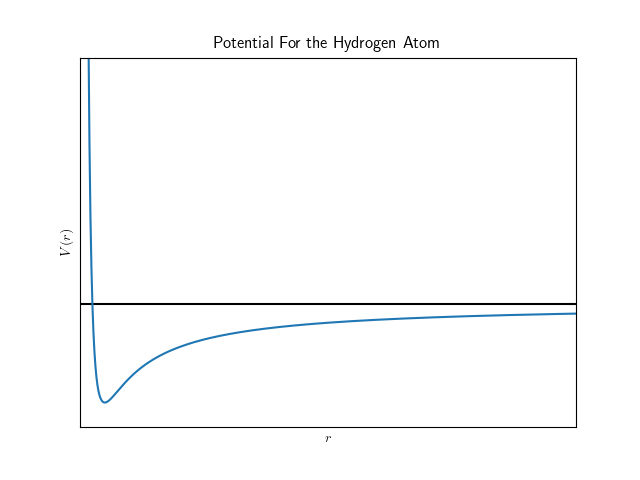
\includegraphics[scale=0.6]{hydrogen_potential.png}
    \caption{The potential for the hydrogen atom.}
    \label{fig:hydrogen atom potential}
\end{figure}

To tidy away even more constants we define
\[a_0 = \frac{\hbar^2}{\mu e^2} \approx \SI{0.52}{\angstrom}, \qquad \text{and} \qquad E_I = \frac{\hbar^2}{2\mu a_0^2} = \frac{\mu e^4}{2\hbar^2} \approx \SI{13.6}{\electronvolt}.\]
\(a_0\) is called the Bohr radius.
We will see the physical significance of these values later.
We now use these quantities to rescale the physical properties of the system:
\[\rho = \frac{r}{a_0}, \qquad\text{and}\qquad \lambda_\ell = \sqrt{-\frac{E_\ell}{E_I}}.\]
Note that since \(E_\ell < 0\) for a bound electron \(\lambda\in\reals\).
We also define \(u_\ell(\rho) = \chi_\ell(\rho)\).
Using this we have
\begin{align*}
    -\lambda_\ell^2E_I\chi(a_0\rho) &= -\lambda_\ell^2E_I u_\ell(\rho)\\
    &= \left[-\frac{\hbar^2}{2\mu}\frac{1}{a_0^2}\dv[2]{\rho} + \frac{\hbar^2\ell(\ell + 1)}{2\mu a_0^2\rho^2} - \frac{e^2}{a_0\rho}\right]\chi_\ell(a_0\rho)\\
    &= \left[-\frac{\hbar^2}{2\mu}\frac{1}{a_0^2}\dv[2]{\rho} + \frac{\hbar^2\ell(\ell + 1)}{2\mu a_0^2\rho^2} - \frac{e^2}{a_0\rho}\right]u_\ell(\rho).
\end{align*}
Which gives us
\[\left[-\frac{\hbar^2}{2\mu}\frac{1}{a_0^2}\dv[2]{\rho} + \frac{\hbar^2\ell(\ell + 1)}{2\mu a_0^2\rho^2} - \frac{e^2}{a_0\rho} + \lambda_\ell^2E_I\right]u_\ell(\rho) = 0.\]
Dividing through by \(-\hbar^2/2\mu a_0^2\) we have
\[\left[\dv[2]{\rho} - \frac{\ell(\ell + 1)}{\rho^2} + \frac{2\mu a_0e^2}{\hbar^2\rho} - \lambda_\ell^2\frac{2\mu a_0^2E_I}{\hbar^2}\right]u_\ell(\rho) = 0.\]
Using the definitions of \(a_0\) and \(E_I\) this becomes
\[\left[\dv[2]{\rho} - \frac{\ell(\ell + 1)}{\rho^2} + \frac{2}{\rho} - \lambda_\ell^2\right]u_\ell(\rho) = 0.\]

\subsubsection{Solution to the Radial Equation}
To motivate an ansatz we will look at the limiting behaviour of the radial equation.
First consider the case that \(\rho \to \infty\), in this case the radial equation reduces to
\[\left[\dv[2]{\rho} - \lambda^2\right]u_\ell(\rho) = 0.\]
The solutions to this are
\[u_\ell(\rho) = e^{\pm\lambda_\ell\rho}.\]
We discard the exponential growth solution as it is non-normalisable so we are left only with the exponential decay solution.
It makes sense for the radial solution to decay exponentially as it becomes increasingly unlikely for the electron to be found as we move away from the proton.
We make the ansatz that
\[u_\ell(\rho) = e^{-\lambda_\ell\rho}\eta_\ell(\rho).\]
Substituting this into the radial equation we have
\begin{align*}
    0 &= \dv[2]{\rho}[e^{-\lambda_\ell\rho}\eta_\ell(\rho)] + \left[\frac{2}{\rho} - \frac{\ell(\ell + 1)}{\rho^2} - \lambda_\ell^2\right]e^{-\lambda_\ell\rho}\eta_\ell(\rho)\\
    &= \dv[2]{\eta_\ell}{\rho}e^{-\lambda_\ell\rho} + 2\dv{\eta_\ell}{\rho}\dv{\rho}e^{-\lambda_\ell\rho} + \eta_\ell(\rho)\dv[2]{\rho}e^{-\lambda_\ell\rho} + \left[\frac{2}{\rho} - \frac{\ell(\ell + 1)}{\rho^2} - \lambda_\ell^2\right]e^{-\lambda_\ell\rho}\eta_\ell(\rho)\\
    &= \dv[2]{\eta_\ell}{\rho}e^{-\lambda_\ell\rho} -2\lambda_\ell 2\dv{\eta_\ell}{\rho}e^{-\lambda_\ell} + \lambda_\ell^2\eta_\ell(\rho)e^{-\lambda_\ell\rho} + + \left[\frac{2}{\rho} - \frac{\ell(\ell + 1)}{\rho^2} - \lambda_\ell^2\right]e^{-\lambda_\ell\rho}\eta_\ell(\rho).\\
\end{align*}
Dividing through by \(e^{-\lambda_\ell\rho}\) we have
\begin{equation}\label{eqn:radial eqn in eta}
    \dv[2]{\eta_\ell}{\rho} - 2\lambda_\ell\dv{\eta_\ell}{\rho} +  \left[\frac{2}{\rho} - \frac{\ell(\ell + 1)}{\rho^2}\right]\eta_\ell(\rho) = 0.
\end{equation}

Now as \(\rho\to 0\) we know from section~\ref{sec:behaviour near the origin central potential} that \(u_\ell(\rho)\sim \rho^{\ell + 1}\).
We expand \(\eta_\ell\) as a power series in \(\rho\) as
\[\eta_\ell(\rho) = \rho^{\ell + 1}\sum_{q = 0}^{\infty} c_q\rho^q.\]
Inserting this into equation~\ref{eqn:radial eqn in eta} we have
\begin{align*}
    0 &= \sum_q \left[(q + \ell + 1)(q + \ell)c_q\rho^{q + \ell - 1} - 2\lambda_\ell(q + \ell + 1)c_q\rho^{\ell + 1} + 2c_q\rho^{q + \ell} - \ell(\ell + 1)c_q\rho^{q + \ell - 1}\right]\\
    &= \sum_q q(q + 2\ell + 1)c_q\rho^{q + \ell - 1} - \sum_q 2(\lambda_\ell[q + \ell + 1] - 1)c_q\rho^{q + \ell}
    \shortintertext{relabelling, \(q \to q - 1\) in the second sum we have}
    &= \sum_q\left[q(q + 2\ell + 1)c_q - 2[\lambda_\ell(q + \ell) - 1]c_{q-1}\right]\rho^{q + \ell - 1}.
\end{align*}
Since we require this to hold for all \(\rho\) we have that for all \(q\)
\begin{equation}\label{eqn:recursion relation}
    q(q + 2\ell + 1)c_q - 2[\lambda_\ell(q + \ell) - 1]c_{q-1} = 0.
\end{equation}
This gives us a recursion relation between the coefficients of the Taylor expansion of \(\eta_\ell(\rho)/\rho^{\ell + 1}\).
For large \(q\) we have
\[\frac{c_q}{c_{q-1}} = \frac{2\lambda_\ell(q + 1) - 2}{q(q + 2\ell + 1)} \to \frac{2\lambda}{q}\]
as \(q \to \infty\) we have
\[c_q \sim c_{q-1}\frac{2\lambda}{q} \sim \frac{(2\lambda_\ell)^q}{q!}.\]
This is the asymptotic behaviour that we expect to give exponential growth in a Taylor series so we expect \(\eta_\ell(\rho) \sim \rho^{\ell + 1}e^{2\lambda\rho}\).
However this is not normalisable.
The only way for this to be normalisable is if for some \(q = n_r\) we have \(c_{n_r} = 0\) as this means that \(c_q = 0\) for all \(q \ge n_r\).
This means that \(\eta_\ell\) is a polynomial of order \(n_r\).
Setting \(q = n_r\) in equation~\ref{eqn:recursion relation} we have that
\[2[\lambda_{n\ell}(n_r + 1) - 1]c_{n_r-1} = 0 \implies \lambda_{n\ell} = \frac{1}{n_r + \ell} = \frac{1}{n}.\]
Here we introduce \(n\), the \define{principle quantum number}.
We see that \(\lambda_{n\ell}\) is quantised as a result of requiring the wave function be normalisable.

\subsubsection{Physical Interpretation}
Since \(\lambda_{n\ell}\) is quantised the energy is also quantised as
\[E_{n\ell} = -\frac{E_I}{(n_r + \ell)^2} = -\frac{E_I}{n^2}.\]
We see that \(E_I\) is the energy needed to remove an electron from the ground state, \(n = 1\).
That is \(E_I\) is the ionisation energy of hydrogen.
Going back to the definition of \(E_I\) we can write
\[E_I = \frac{\mu e^4}{2\hbar^2} = \frac{1}{2}\alpha^2\mu c^2\]
where
\[\alpha = \frac{e^2}{\hbar c^2} = \frac{q^2}{4\pi\varepsilon_0\hbar c} \approx \frac{1}{137}\]
is the \define{fine-structure constant}.
Notice that \(\mu \approx m_e\) and therefore \(\mu c^2\) is approximately the rest energy of the electron.
The energy levels are on the scale of \(\alpha^2\mu c^2/2 \approx \mu c^2 \num{2.7e-5}\).
Since the energy levels are on a scale so much smaller than the rest mass of the electron (which is in turn much less than the rest energy of the proton) we are justified in using a non-relativistic approach.
Any relativistic corrections will typically be \(\order{(\alpha)}\).
Further justification is provided by Heisenberg's uncertainty principle.
Taking \(a_0\) to be a typical length scale in hydrogen we have that \(\Delta p \approx a_0\hbar/2 = \mu e^2/\hbar\).
We can also use the symmetry to state that positive and negative momenta are equally likely so \(\Delta p = \sqrt{\expected{p^2} - \expected{p}^2} = \sqrt{\expected{p^2}}\) from which we have
\[v \sim \frac{p}{\mu} \sim \frac{e^2}{\hbar} = \alpha c \approx \frac{1}{137}c \ll c.\]
So we see that once again relativity only comes into play on scales less than \(a_0\).
Any relativistic corrections are going to be on the order of \(\order{(v/c)} = \order{(\alpha)}\).

We can write the energy levels further as
\[E_n = -\frac{e^2}{2n^2a_0} = -\frac{\mu e^4}{2n^2\hbar^2} = -\frac{\mu q^4}{32\hbar^2\pi^2\varepsilon_0^2n^2}.\]
From \(n = n_r + \ell\) since \(n, n_r\in\naturals_{>0}\) we have that \(\ell = 0, 1, \dotsc, n - 1\), which corresponds to \(n_r = n, n-1, \dotsc, 1\).
For a particular value of \(\ell\) we have \((2\ell + 1)\)-fold degeneracy.
This means that the total degeneracy of the eigenvalue \(E_n\) is
\[g_n = \sum_{\ell = 0}^{n - 1}(2\ell + 1) = 2\sum_{\ell=0}^{n-1}\ell + \sum_{\ell=0}^{n-1}1 = (n - 1)n + n = n^2.\]
Here we have used the result proven in section~\ref{sec:proof sum 0 to n of r is 0.5 n(n+1)}.
The fact that \(E_n = E_I/n^2\) was first proposed by Niels Bohr in 1913 before the full quantum picture that we have seen here was known.
However quantum mechanics is still needed to find the degeneracy of \(E_n\) and other important properties.

The full radial wave function is
\[R_{n\ell}(r) = \frac{\chi_{n\ell}(r)}{r} = \frac{u_{n\ell}(a_0\rho)}{a_0\rho} = \frac{1}{a_0\rho}e^{-\lambda\rho}\eta_{n\ell}(\rho) = \frac{1}{a_0\rho}e^{-\lambda\rho}\sum_{q=0}^{n_r} c_q\rho^{q + \ell + 1}.\]
The polynomials in the last term are called the \define{associated Laguerre polynomials}.
They can be looked up in standard texts.
If we do this we find that
\begin{align*}
    R_{1,0}(r) &= \frac{2}{a^{3/2}}e^{-r/a_0}\\
    R_{2,0}(r) &= \frac{1}{2\sqrt{2}} \frac{1}{a^{3/2}} \left[2 - \frac{r}{a_0}\right] e^{-r/(2a_0)}\\
    R_{2,1}(r) &= \frac{1}{2\sqrt{6}} \frac{1}{a^{3/2}} \frac{r}{a_0} e^{-r/(2a_0)}.
\end{align*}
Notice that \(R\sim a_0^{-3/2}\) so \(\abs{R}^2\sim a_0^3\).
This means that \(\abs{R}\) has units of probability per unit volume, which is what we want since \(\psi = RY_\ell^m\) is a probability density and \(Y_\ell^m\) is dimensionless.

\section{Non-degenerate Time-Independent Perturbation Theory}
Many problems in quantum mechanics involve solving the \gls{tise}.
In most cases however an analytic solution does not exist.
If this is the case then the best we can do is find an estimate.
One of the most common ways to do this is perturbation theory.
This gives us a way to solve the \gls{tise} for a system with a Hamiltonian of the form
\[\operator{H} = \operator{H}_0 + \varepsilon\operator{V}.\]
Here \(\operator{H}\) is the Hamiltonian we wish to find a solution for, \(\operator{H}_0\) is a Hamiltonian for which we know the solution to the \gls{tise} and \(\operator{V}\) is known as a perturbation.
We will assume that \(\operator{H}\) and \(\operator{H}_0\) have discrete, non-degenerate eigenvalues.
Let \(\ket{\varphi_n}\) be the eigenstate of \(\operator{H}_0\) with eigenvalue \(E_n^{(0)}\), i.e.
\[\operator{H}_0\ket{\varphi_n} = E_n^{(0)}\ket{\varphi_n}.\]
We want to find \(\ket{\psi_n}\) and \(E_n\) such that
\[\operator{H}\ket{\psi_n} = E_n\ket{\psi_n}.\]
We look for a solution expanded in terms of \(\varepsilon\).
We can expand the energy as
\[E_n = E_{0n} + \varepsilon E_{1n} + \varepsilon^2E_{2n} + \order{\varepsilon^3} = \sum_{k=1}^{\infty} \varepsilon^kE_{kn},\]
where \(E_{kn}\) are to be found.
Similarly we can expand the eigenstate as
\[\ket{\psi_n} = \ket{\psi_{0n}} + \varepsilon\ket{\psi_{1n}} + \varepsilon^2\ket{\psi_{2n}} + \order{\varepsilon^3} = \sum_{k=1}^{\infty} \varepsilon^k\ket{\psi_{kn}},\]
where \(\ket{\psi_{kn}}\) are to be found.
Inserting these expansions and the definition of \(\operator{H}\) into the \gls{tise} we find that
\[(\operator{H}_0 + \varepsilon\operator{V})\sum_{i=1}^{\infty}\ket{\psi_{in}} = \left[\sum_{j=1}^{\infty}E_{jn}\right]\left[\sum_{k=1}^{\infty}\ket{\psi_{kn}}\right].\]
Expanding these sums up to second order in \(\varepsilon\) we have
\begin{multline*}
    \operator{H}_0\ket{\psi_{0n}} + \varepsilon(\operator{H}_0\ket{\psi_{1n}} + \operator{V}\ket{\psi_{0n}}) + \varepsilon^2(\operator{H}_0\ket{\psi_{2n}} + \operator{V}\ket{\psi_{1n}}) + \order{\varepsilon^3} =\\
    E_{0n}\ket{\psi_{0n}} + \varepsilon(E_{0n}\ket{\psi_{1n}} + E_{1n}\ket{\psi_{0n}}) + \varepsilon^2(E_{0n}\ket{\psi_{2n}} + E_{1n}\ket{\psi_{1n}} + E_{2n}\ket{\psi_{0n}}) + \order{\varepsilon^3}.
\end{multline*}
\subsection{Zeroth Order}
Equating coefficients of terms of zeroth order in \(\varepsilon\) we have
\[\operator{H}_0\ket{\psi_{0n}} = E_{0n}\ket{\psi_{0n}}.\]
Notice that this is exactly what we would get if \(\varepsilon = 0\) so this is just the unperturbed Hamiltonian meaning that \(\ket{\psi_{0n}} = \ket{\varphi_n}\) and \(E_{0n} = E_n^{(0)}\).

\subsection{First Order}
\subsubsection{Energy Perturbation}
Equating coefficients of terms of first order in \(\varepsilon\) we have
\[\operator{H}_0\ket{\psi_{1n}} + \operator{V}\ket{\psi_{0n}} = E_{0n}\ket{\psi_{1n}} + E_{1n}\ket{\psi_{0n}}.\]
Rearranging this we have
\begin{equation}\label{eqn:perturbation theory first order terms}
    (\operator{H} - E_{0n})\ket{\psi_{1n}} - (\operator{V} - E_{1n})\ket{\psi_{0n}} = 0.
\end{equation}
We then take an inner product with \(\ket{\psi_{0n}}\):
\[\bra{\psi_{0n}}\operator{H}_0\ket{\psi_{1n}} - E_{0n}\braket{\psi_{0n}}{\psi_{1n}} - \bra{\psi_{0n}}\operator{V}\ket{\psi_{0n}} + E_{1n}\braket{\psi_{0n}}{\psi_{0n}} = 0.\]
Consider the first term of this sum:
\begin{align*}
    \bra{\psi_{0n}}\operator{H}_0\ket{\psi_{1n}} &= (\bra{\psi_{1n}}\operator{H}_0\hermit\ket{\psi_{0n}})^*\\
    &= (\bra{\psi_{1n}}\operator{H}_0\ket{\psi_{0n}})^*\\
    &= E_{0n}(\braket{\psi_{1n}}{\psi_{0n}})^*\\
    &= E_{0n}\braket{\psi_{0n}}{\psi_{1n}}.
\end{align*}
So the first term cancels with the second, note that we make no assumptions about \(\ket{\psi_{kn}}\) being orthonormal.
Rearranging the remaining two terms we have
\[E_{1n} = \frac{\bra{\psi_{0n}}\operator{V}\ket{\psi_{0n}}}{\braket{\psi_{0n}}{\psi_{0n}}} = \frac{\bra{\varphi_n}\operator{V}\ket{\varphi_n}}{\braket{\varphi_n}{\varphi_n}} = V_{00},\]
where \(V\) is a matrix representation of \(\operator{V}\) and we assume that \(\ket{\psi_n}\) are orthonormal.
Note that since \(E_{0n}\) is a shift in the energy to first order it is sometimes written as \(\Delta E_{0n}\).

\subsubsection{Eigenstate Perturbation}
We can express \(\ket{\psi_{1n}}\) in the energy eigenbasis of \(\operator{H}_0\):
\[\ket{\psi_{1n}} = \sum_{m}c_m\ket{\varphi_m},\]
where as usual \(c_m = \braket{\varphi_m}{\psi_{1n}}\).
We can take a scalar product of equation~\ref{eqn:perturbation theory first order terms} with \(\ket{\varphi_m}\) and we get
\[\bra{\varphi_m}\operator{H}_0\ket{\psi_{1n}} - E_{0n}\braket{\varphi_m}{\psi_{1n}} + \bra{\varphi_m}\operator{V}\ket{\varphi_n} + E_{1n}\braket{\varphi_m}{\varphi_n} = 0.\]
We will first consider the case when \(m \ne n\), thus the last term is zero.
Analogously to how we worked with the first term for the energy perturbation we can show that the first term is simply \(E_{0m}\braket{\varphi_m}{\psi_{1n}}\).
Thus
\[(E_{0m} - E_{0n})\braket{\varphi_m}{\psi_{1n}} + \bra{\varphi_m}\operator{V}\ket{\varphi_n}.\]
Hence
\[c_m = \braket{\varphi_m}{\psi_{1n}} = \frac{\bra{\varphi_m}\operator{V}\ket{\varphi_n}}{E_{0n} - E_{0m}} = \frac{V_{mn}}{E_{0n - E_0m}}.\]
Note that \(E_{0n} = E_n^{(0)}\) and \(E_{0m} = E_m^{(0)}\) are simply the \(n\)th and \(m\)th energy eigenvalues of \(\operator{H}_0\) so are known quantities.
Knowing this we can express the \(n\)th perturbed eigenstate, \(\ket{\psi_{n}}\), as
\[\ket{\psi_{n}} = \ket{\varphi_n} + \varepsilon\sum_{m\ne n}\frac{V_{mn}}{E_{0n} - E_{0m}}\ket{\varphi_m} + \varepsilon c_n\ket{\varphi_n} + \order{\varepsilon^2}.\]
So to find the adjustment needed at first order we just need to compute \(c_n\) which we can do by imposing normalisation, taking the inner product of this with \(\ket{\psi_{n}}\) we have
\[1 = \braket{\psi_{n}}{\psi_{n}} = 1 + 2\varepsilon c_n\braket{\varphi_n}{\varphi_n} + \order{\varepsilon^2},\]
where we have used the fact that \(\ket{\varphi_n}\) are orthonormal so \(\braket{\varphi_n}{\varphi_m} = \delta_{nm}\) meaning that the inner product with the sum term gives zero as \(\ket{\varphi_n}\) is explicitly excluded from that sum.
From this we conclude that we must have \(c_n = 0\), so \(\ket{\psi_{1n}}\) has no component in the \(\ket{\varphi_n}\) direction.
Thus
\[\ket{\psi_{1n}} = \sum_{m\ne n} \frac{V_{mn}}{E_{0n} - E_{0m}}\ket{\varphi_m}.\]

\subsection{Second Order}
Equating coefficients of terms of second order in \(\varepsilon\) we have
\[\operator{H}_0\ket{\psi_{2n}} + \operator{V}\ket{\psi_{1n}} = E_{0n}\ket{\psi_{2n}} + E_{1n}\ket{\psi_{1n}} + E_{2n}\ket{\psi_{0n}}.\]
Rearranging this we have
\[(\operator{H}_0 - E_{0n})\ket{\psi_{2n}} + (\operator{V} - E_{1n})\ket{\psi_{1n}} - E_{2n}\ket{\psi_{0n}} = 0.\]
We then take the inner product with \(\ket{\varphi_n}\) and we have
\[\bra{\varphi_n}\operator{H}_{0}\ket{\psi_{2n}} - E_{0n}\braket{\varphi_n}{\psi_{2n}} + \bra{\varphi_n}\operator{V}\ket{\psi_{1n}} - E_{1n}\braket{\varphi_n}{\psi_{1n}} - E_{2n}\braket{\varphi_n}{\psi_{0n}} = 0.\]
The first term is equal to \(E_{0n}\braket{\varphi_n}{\psi_{2n}}\) so combines with the second term to give zero.
The fourth term is zero as \(\ket{\psi_{1n}}\) has no \(\ket{\varphi_n}\) component.
The scalar product in the fifth term is simply one as \(\ket{\psi_{0n}} = \ket{\varphi_n}\).
Thus
\begin{align*}
    E_{2n} &= \bra{\varphi_n}\operator{V}\ket{\psi_{1n}}\\
    &= \bra{\varphi_n}\operator{V}\sum_{m\ne n} \frac{V_{mn}}{E_{0n} - E_{0m}}\ket{\varphi_m}\\
    &= \sum_{m\ne n}\frac{V_{mn}}{E_{0n} - E_{0m}}\bra{\varphi_n} \operator{V}\ket{\varphi_m}\\
    &= \sum_{m\ne n}\frac{V_{mn}V_{nm}}{E_{0n} - E_{0m}}\\
    &= \sum_{m\ne n}\frac{\abs{V_{mn}^2}}{E_{0n} - E_{0m}}.
\end{align*}

\subsection{Perturbation Examples}
\subsubsection{Infinite Well With a Cosine Floor}
Consider the potential
\[
V(x) = 
\begin{cases}
    V_0\cos\left(\frac{\pi x}{2a}\right), & \abs{x} \le a,\\
    \infty, & \abs{x} > a.
\end{cases}
\]
If we define \(\operator{H}'\) as
\[V_0 \cos\left(\frac{\pi x}{2a}\right)\]
then we can view the Hamiltonian for this system as
\[\operator{H} = \operator{H}_0 + \operator{H}'\]
where \(\operator{H}_0\) is the Hamiltonian for an infinite square well.
The solution to the \gls{tise} for the infinite square well is discussed in section~\ref{sec:infinite square well}.
In particular the \(n\)th energy level is
\[E_n^{(0)} = \frac{\hbar^2\pi^2 n^2}{8ma^2},\]
and the corresponding eigenfunction is
\[
\varphi_{(n)}(x) =
\begin{cases}
    \frac{1}{\sqrt{a}}\cos\left(\frac{n\pi x}{2a}\right), & \text{for odd}~n,\\
    \frac{1}{\sqrt{a}}\sin\left(\frac{n\pi x}{2a}\right), & \text{for even}~n.
\end{cases}
\]
Perturbation theory only gives a good estimate if the energy shift due to the addition of \(\operator{H}'\) to the Hamiltonian is small, in this case this means that we require \(V_0 \ll E_0^{(2)} - E_0^{(1)}\).
The energy shift is then
\begin{align*}
    \Delta E_1 &= \bra{\varphi^{(1)}}\operator{H}'\ket{\varphi^{(1)}}\\
    &= \int_{-a}^{a} \varphi^{(1)}(x)^*V_0\cos\left(\frac{\pi x}{2a}\right)\varphi^{(1)} (x)\dd{x}\\
    &= \frac{V_0}{a} \int_{-a}^{a} \cos^3\left(\frac{\pi x}{2a}\right) \dd{x}\\
    &= \frac{8V_0}{3\pi}.
\end{align*}
So to first order the energy of the ground state is
\[E_1 = E_1^{(0)} + \Delta E_1 = \frac{\hbar^2\pi^2 n^2}{8ma^2} + \frac{8V_0}{3\pi}.\]

\subsubsection{Helium}
Helium is a two electron atom.
If we ignore the interaction between the electrons then the Hamiltonian for a helium atom is
\[\operator{H}_0 = \frac{\hbar^2}{2m}\laplacian_1 - \frac{Ze^2}{r_1} + \frac{\hbar^2}{2m}\laplacian_2 - \frac{Ze^2}{r_2} = \operator{H}_0^{(1)} + \operator{H}_0^{(2)}.\]
Here \(m\) is the reduced mass of an electron and the nucleus,
\[\frac{1}{m} = \frac{1}{m_e} + \frac{1}{2m_p} \approx \frac{1}{m_e}.\]
The distances \(r_1\) and \(r_2\) are the distances from the nucleus to the relevant electron, where we model the four nucleon nucleus as a point charge of charge \(Z = 2e\).
The Laplacian operator, \(\laplacian_1\) or \(\laplacian_2\), acts only on the coordinates of the relevant electron.

The Hamiltonian is independent of the spin of any one part of the system.
This means that we can treat the spin of the electrons as we do for a normal two particle, spin 1, system.
A generic state, \(\ket{\Psi}\in \hilbert\) can be described by \(\ket{\psi}\in\hilbert_{\text{space}}\) and \(\ket{s, s_z}\in\hilbert_{\text{spin}}\) as
\[\ket{\Psi} = \ket{\psi} \tensorProd \ket{s, s_z} = \ket{\psi; s, s_z}.\]
As discussed in section~\ref{sec:total angular momentum}
\[\ket{s=1, s_z=1} = \ket{\spinUp\spinUp}, \qquad \ket{s=1, s_z=-1} = \ket{\spinDown\spinDown}, \qquad\ket{s=1, s_z=0} = \frac{\sqrt{2}}{2}(\ket{\spinUp\spinDown} + \ket{\spinDown\spinUp}),\]
\[\text{and}\qquad \ket{s=0, s_z=0} = \frac{\sqrt{2}}{2}(\ket{\spinUp\spinDown} - \ket{\spinDown\spinUp}).\]
The spatial wave function is given by
\[\braket{\vv{r_1}, \vv{r_2}}{\psi} = \psi(\vv{r_1}, \vv{r_2}) = \psi^{(1)}(\vv{r_1})\psi^{(2)}(\vv{r_2}),\]
where we assume in the last step that a separable solution exists.
Each \(\psi^{(k)}\) must satisfy the \gls{tise} for the relevant Hamiltonian:
\[\operator{H}_0^{(k)}\psi^{(k)}(\vv{r_k}) = \left[\frac{\hbar^2}{2m}\laplacian_k - \frac{Ze^2}{r_k}\right]\psi^{(k)}(\vv{r_k}) = E^{(k)}\psi^{(k)}(\vv{r_k}).\]
This is simply the \gls{tise} that we solved for the hydrogen atom but with the nucleus charge changed to \(Z = 2e\) instead of \(Z = e\).
The solutions to this are the states \(u_{n\ell m}\), where the ground state is
\[\psi^{(k)}(\vv{r_k}) = u_{100}(\vv{r_k}) = \frac{1}{\sqrt{\pi}} \left(\frac{Z}{a_0}\right)^{3/2}e^{-r/a_0}.\]
Thus
\[\braket{\vv{r_1}, \vv{r_2}}{\Psi} = u_{100}(\vv{r_1})u_{100}(\vv{r_2})\sum_{\alpha = 1}^{4}c_\alpha\ket{\alpha}\]
where
\[\{\ket{\alpha}\} = \{\ket{s, s_z}\st s = 0, 1~\text{and}~s_z = -s, \dotsc, s\}.\]
Electrons are fermions.
This means that \(\ket{\Psi}\) should be antisymmetric under exchanging of 1 and 2.
The radial part, \(u_{100}(\vv{r_1})u_{100}(\vv{r_2})\), is symmetric under exchanging of 1 and 2 so the spin part must be antisymmetric.
The only antisymmetric spin state available is \(\ket{s = 0, s_z = 0}\).

We are now in a position to consider what happens when we include the interaction between the electrons.
This interaction is characterised by the potential
\[\operator{V} = \frac{e^2}{\abs{\vv{r_1} - \vv{r_2}}}.\]
The energy shift due to this perturbation is
\begin{align*}
    \Delta E_1 &= \bra{\Psi}\operator{V}\ket{\Psi}\\
    &= \bra{\psi; 0, 0}\operator{V}\ket{\psi; 0, 0}
    \shortintertext{using the fact that \(\operator{V}\) acts only on the radial part this becomes}
    &= \braket{0, 0}{0, 0}\bra{\psi}\operator{V}\ket{\psi}
    \shortintertext{considering the ground state, \(\psi(\vv{r}) = u_{100}(\vv{r})\), or equivalently \(\ket{\psi} = \ket{100}\), this becomes}
    &= \bra{100, 100}\operator{V}\ket{100, 100}\\
    &= \int \dd[3]{r_1}\dd[3]{r_2} u_{100}^*(\vv{r_1})u_{100}^*(\vv{r_2})\frac{e^2}{\abs{\vv{r_1} - \vv{r_2}}}u_{100}(\vv{r_1})u_{100}(\vv{r_2})\\
    &= \left(\frac{eZ^3}{\pi a_0^3}\right)^2 \int \dd[3]{r_1}\dd[3]{r_2} \exp\left(-\frac{2Z(r_1 + r_2)}{a_0}\right)\frac{1}{\abs{\vv{r_1} - \vv{r_2}}}\\
    &= \frac{5}{4}ZE_I
\end{align*}
where \(E_I \approx \SI{13.6}{\electronvolt}\) is defined as it was in section~\ref{sec:stationary states hydrogen atom}.
    \part{Recap}
\section{Recap Part One}
\setcounter{postulateCounter}{0}
\begin{postulate}{}{}
    Every possible physical state of a given system corresponds to some state vector, \(\ket{\Psi(t)} \in \hilbert\), from which all possible predictions of the physical properties of the system can be obtained.
\end{postulate}
The state vector can often be represented by a wave function, \(\Psi(\vv{r}, t) = \braket{\vv{r}}{\Psi(t)}\), however this is not always the case.
For example the spin of a system cannot be represented in this way and we instead represent spin with column vectors.

\begin{postulate}{}{}
    Every physical observable is represented by a Hermitian operator.
    For each observable, \(\observable{A}\), there is a Hermitian operator, \(\operator{A}\), with a complete orthonormal set of eigenfunctions, \(\{u_i\}\), or eigenvectors, \(\{\ket{u_i}\}\), or generically eigenstates, which have a corresponding set of real eigenvalues, \(\{A_i\}\), such that
    \[\operator{A}u_i(\vv{r}) = A_iu_i(\vv{r}), \qquad\text{or}\qquad \operator{A}\ket{u_i} = A_i\ket{u_i}.\]
    The set of possible values that a measurement of \(\observable{A}\) can yield is identically \(\{A_i\}\).
\end{postulate}

The Hermitian conjugate of an operator, \(\operator{O}\), is \(\operator{O}\hermit\), which is defined by
\[\left(\int\psi^*\operator{O}\varphi \dd[3]{r}\right)^* = \int \varphi^*\operator{O}\hermit\psi\dd[3]{r} \qquad\text{or}\qquad \bra{\psi}\operator{O}\ket{\varphi}^* = \bra{\varphi}\operator{O}\hermit\ket{\psi},\]
where \(\ket{\varphi}, \ket{\psi}\in\hilbert\) are arbitrary states.
The operator \(\operator{O}\) is Hermitian if \(\operator{O}\hermit = \operator{O}\).

States, \(\{u_i\}\) or \(\{\ket{u_i}\}\), are orthonormal if
\[\int u_i^*(\vv{r})u_j(\vv{r}) \dd[3]{r} = \delta_{ij}, \qquad\text{or}\qquad \braket{u_i}{u_j} = \delta_{ij}.\]
A set of states, \(\{u_i\}\) or \(\{\ket{u_i}\}\), is complete if an arbitrary state, \(\Psi(\vv{r}, t)\) or \(\ket{\Psi(t)}\), can be represented by
\[\Psi(\vv{r}, t) = \sum_{i} c_i(t)u_i(\vv{r}), \qquad\text{or}\qquad \ket{\Psi(t)} = \sum_{i} c_i(t)\ket{u_i}.\]
The coefficients \(\{c_i\}\) are given by
\[c_i(t) = \int u_i^{*}(\vv{r})\Psi(\vv{r}, t)\dd[3]{r}, \qquad\text{or}\qquad c_i(t) = \braket{u_i}{\Psi(t)}.\]
Compare this to some vector \(\vv{v}\in\reals^n\) where \(\vv{v} = \sum_i v_i\ve{i}\) with \(v_i = \ve{i}\cdot\vv{v}\).
The set of eigenfunctions, \(\{u_i\}\), or eigenvectors, \(\{\ket{u_i}\}\), is referred to as the eigenbasis of \(\operator{A}\).
Comparing the equations for \(\Psi(\vv{r}, t)\) or \(\ket{\Psi(t)}\) and \(c_i(t)\) we see that
\[\ket{\Psi(t)} = \sum_{i} \bra{u_i}\braket{u_i}{\Psi(t)}\]
and so the completeness relation,
\[\sum_{i}\ket{u_i}\bra{u_i} = \ident\]
where \(\ident\) is the identity operator defined by
\[\ident\ket{\Psi} = \ket{\Psi}\]
for all \(\ket{\Psi}\).

The spectrum of eigenvalues of \(\operator{A}\) may be discrete (which we assumed was the case above) or continuous.
For example the angular momentum operators \(\operator{L}^2\) and \(\operator{L}_z\) have discrete spectra whereas the position, \(\operator{X}\) and momenta \(\operator{P}\) have continuous spectra and the energy, \(\operator{H}\), has a spectrum that is continuous in some cases and discrete in other cases.

Observables can be represented by differential operators acting on the wave function or as Hermitian matrices acting on column vectors, for example
\[
\operator{P} \representation -i\hbar\grad, \qquad\text{and}\qquad \operator{S}_z \representation \frac{1}{2}\hbar
\begin{pmatrix}
    1 & 0\\
    0 & -1
\end{pmatrix}
\]

\begin{postulate}{}{}
    If the observable \(\observable{A}\) is measured on a system which, immediately prior to the measurement, is in the state \(\ket{\Psi(t)}\) then the strongest predictive statement we can make about the result is that the probability of measuring \(\observable{A}\) to be \(A_i\) is
    \[P(A_i) = \abs{\braket{u_i}{\Psi(t)}}^2 = \abs{c_i(t)}^2.\]
\end{postulate}
This assumes that the state \(\ket{\Psi(t)}\) is normalised so that
\[\abs{\braket{\Psi(t)}{\Psi(t)}}^2 = \sum_i \abs{\braket{u_i}{\Psi(t)}}^2 = \sum_i \abs{c_i(t)}^2 = 1.\]
We also assume that measurements are ideal and yield a single, errorless, number.

The coefficients, \(c_i(t)\), are called the probability amplitudes.
In general we cannot predict with certainty the outcome of a measurement unless \(\ket{\Psi(t)}\) happens to coincide with an eigenstate of \(\operator{A}\).

\subsection{Repeated Measurements}
Repeated measurements are measurements made on the same state, \(\ket{\Psi(t)}\).
We imagine creating an assembly of an infinite number of identical systems and performing each measurement on a different one of these systems.
The average value of this process, if all measurements are completed at time \(t\), is
\[\expected{\operator{A}}_t = \int \Psi^*(\vv{r}, t)\operator{A}\Psi(\vv{r}, t)\dd[3]{r}, \qquad\text{or}\qquad \expected{\operator{A}}_t = \bra{\Psi(t)}\operator{A}\ket{\Psi(t)}.\]
If we expand \(\ket{\Psi(t)}\) in the eigenstates of \(\operator{A}\) then we see that
\begin{align*}
    \expected{\operator{A}}_t &= \sum_{i, j} c_i^*(t)c_j(t)\bra{u_i}\operator{A}\ket{u_j}\\
    &= \sum_{i, j} c_i^*(t)c_j(t) A_j\braket{u_i}{u_j}\\
    &= \sum_{i, j} c_i^*(t)c_j(t) A_j\delta_{ij}\\
    &= \sum_{i} \abs{c_i}^2A_i\\
    &= \sum_{i} P(A_i)A_i.
\end{align*}
This is the usual definition of the mean of a discrete variable \(\observable{A}\) which can take values in \(\{A_i\}\).

\subsection{Uncertainty}
The uncertainty is the root mean square deviation about the mean of an infinite amount of repeated measurements.
It is given at time \(t\) by
\[\Delta\operator{A}_t \sqrt{\expected{\operator{A}^2}_t - \expected{\operator{A}}_t^2}.\]
This uncertainty is not due to the way the experiment is conducted or due to missing data.
It is an intrinsic limit to what we can know.

The generalised uncertainty relation states that two observables \(\observable{A}\) and \(\observable{B}\) have uncertainties \(\Delta \operator{A}_t\) and \(\Delta \operator{B}_t\) respectively which satisfy
\[\Delta \operator{A}_t \Delta \operator{B}_t \ge \frac{1}{2}\abs{[\operator{A}, \operator{B}]}\]
where
\[[\operator{A}, \operator{B}] = \operator{A}\operator{B} - \operator{B}\operator{A}\]
is the commutator.
The most important case of this relationship is
\[\Delta\operator{X}_t\Delta\operator{P} \ge \frac{\hbar}{2}.\]

\section{Recap Part Two}
\subsection{Successive Measurements}
Successive measurements refers to measurements made on the same system in quick succession.
\begin{postulate}{}{}
    A measurement of an observable, \(\observable{A}\), generally causes a drastic, uncontrollable change in the state of the system.
    Regardless of the state, \(\ket{\Psi(t)}\), before the measurement immediately after the measurement the state vector will coincide with the eigenstate \(\ket{u_k}\) corresponding to the measured value, \(A_k\), of \(\observable{A}\).
\end{postulate}
This is referred to as collapse of the wave function or reduction of state.
We say that the state is forced or projected into the eigenstate.
This assumes that there is no degeneracy.
If instead \(A_k\) is \(g\)-fold degenerate and the \(g\) eigenstates \(\{\ket{u_i^{(k)}}\}\) all have eigenvalue \(A_k\) then if a system is measured to have \(\observable{A} = A_k\) we will find immediately after this measurement that the state is a linear superposition of the degenerate states:
\[\frac{1}{\sqrt{_{i=1}^{g} \abs{c_i^{(k)}}^2}} \sum_{i=1}^{n} c_i^{(k)}\ket{u_i^{(k)}}.\]

\subsection{Compatible Observables}
If \(\observable{A}\) and \(\observable{B}\) are observables and we perform the following series of measurements,
\begin{enumerate}
    \item Measure \(\observable{A}\),
    \item Measure \(\observable{B}\),
    \item Measure \(\observable{A}\),
\end{enumerate}
then \(\observable{A}\) and \(\observable{B}\) are said to be compatible if and only if the result of the third measurement is guaranteed to be the same as the result of the first measurement.

\begin{theorem}{Compatibility Theorem}{}
    If \(\observable{A}\) and \(\observable{B}\) are observables represented by Hermitian operators \(\operator{A}\) and \(\operator{B}\) respectively then the following are equivalent:
    \begin{itemize}
        \item \(\observable{A}\) and \(\observable{B}\) are compatible observables.
        \item \(\operator{A}\) and \(\operator{B}\) have a common eigenbasis.
        \item \(\operator{A}\) and \(\operator{B}\) commute.
    \end{itemize}
\end{theorem}
A set of variables, \(\{\observable{A}^{(i)}\}\) are called a \acrfull{csco} if the eigenvalues of each observable, \(A_k^{(i)}\), uniquely identify an eigenvector in the common eigenbasis.
For example for a hydrogen atom the set energy, angular momentum squared and the \(z\) component of angular momentum are a \gls{csco} as a state \(\ket{n, \ell, m}\) is uniquely identified by the numbers \(n\), \(\ell\), and \(m\).

\subsection{Time Development}
\begin{postulate}{}{}
    The time development of a quantum system is determined by the \gls{tdse}:
    \[\operator{H}\Psi(\vv{r}, t) = i\hbar\pdv{t}\Psi(\vv{r}, t), \qquad\text{or}\qquad \operator{H}\ket{\Psi(t)} = i\hbar\pdv{t}\ket{\Psi(t)}.\]
    \(\operator{H}\) is the Hamiltonian operator which is formed from the corresponding classical Hamiltonian replacing the variables with corresponding operators.
    \(\operator{H}\) represents the total energy of the system.
\end{postulate}

The wave function can be interpreted as \(\abs{\Psi(\vv{r}, t)}^2\dd[3]{r}\) giving the probability that a measurement of position will give a result in the infinitesimal volume element \(\dd[3]{r}\) at \(\vv{r}\) where the volume element in Cartesian and spherical coordinates is \(\dd[3]{r} = \dd{x}\dd{y}\dd{z = r^2\sin\vartheta\dd{r}\dd{\vartheta}\dd{\varphi}}\).
Hence \(\abs{\Psi(\vv{r}, t)}\) is a probability density.

The classical Hamiltonian is \(H = T + V\).
When constructing the quantum Hamiltonian the momentum, \(\vv{p}\), is substituted for the momentum operator \(\vecoperator{P}\) which has the following representation:
\[\operator{P}_i \representation -i\hbar\pdv{x_i} \implies \vecoperator{P} \representation -i\hbar\grad.\]
For a single particle \(T = p^2/2m = \vv{p}\cdot\vv{p}/2m\) and therefore
\[\operator{T} = \frac{\operator{P}^2}{2m} \representation \frac{\hbar^2}{2m}\laplacian.\]
Most of the time we consider the potential, \(V\), to be a function of position only, \(V = V(\vv{r})\).
The position in the classical Hamiltonian is replaced by the position operator, \(\vecoperator{X}\), which has the following representation:
\[\operator{X}_i = x_i \implies \vecoperator{X} = \vv{r}.\]
Thus
\[\operator{V} \representation V(\vv{r}).\]
So the Hamiltonian operator is given by
\[\operator{H} = \operator{T} + \operator{V} = \frac{\operator{P}^2}{2m} + V(\vecoperator{X}) \representation -\frac{\hbar^2}{2m} + V(\vv{r}).\]
The \gls{tdse} is then
\[\left[-\frac{\hbar^2}{2m}\laplacian + V(\vv{r})\right]\Psi(\vv{r}, t) = i\hbar\pdv{t}\Psi(\vv{r}, t).\]
This has separable solutions of the form
\[\Psi_n(\vv{r}, t) = u_n(\vv{r})\exp(-iE_nt/\hbar).\]
This gives us the \acrfull{tise}:
\[\left[-\frac{\hbar^2}{2m}\laplacian + V(\vv{r})\right]u_n(\vv{r}) = E_nu_n(\vv{r}), \qquad\text{or}\qquad \operator{H}\ket{n} = E_n\ket{n}.\]
This is an eigenvalue equation for \(\operator{H}\) so we see that the stationary states, \(\{\ket{u_n}\}\), correspond to the energy levels.

It can be shown that for an observable \(\observable{A}\) represented by the Hermitian operator \(\operator{A}\)
\[\dv{t}\expected{\operator{A}}_t = \frac{i}{\hbar}\expected{[\operator{H}, \operator{A}]}_t.\]
Importantly if \(\operator{A}\) and \(\operator{H}\) commute then \(\expected{\operator{A}}_t\) is constant.

\subsection{Angular Momentum}
The classical angular momentum, \(\vv{L} = \vv{r}\times\vv{p}\), under operator substitution becomes the angular momentum operator
\[\vecoperator{L} = \vecoperator{X}\times\vecoperator{P}\]
which has components
\[\operator{L}_x \representation -i\hbar\left(y\pdv{z} - z\pdv{y}\right), \qquad \operator{L}_y \representation -i\hbar\left(z\pdv{x} - x\pdv{z}\right), \qquad\text{and}\qquad \operator{L}_z \representation -i\hbar\left(x\pdv{y} - y\pdv{x}\right).\]
More compactly:
\[\operator{L}_k \representation -i\hbar\varepsilon_{ijk}x_i\pdv{x_j}.\]
These satisfy the commutation relations
\[[\operator{L}_x, \operator{L}_y] = i\hbar\operator{L}_z, \qquad [\operator{L}_y, \operator{L}_z] = i\hbar\operator{L}_x, \qquad\text{and}\qquad [\operator{L}_z, \operator{L}_x] = i\hbar\operator{L}_y.\]
More compactly
\[[\operator{L}_i, \operator{L}_j] = i\varepsilon_{ijk}\operator{L}_k.\]
We also define
\[\operator{L}^2 = \operator{L}_x^2 + \operator{L}_y^2 + \operator{L}_z^2.\]
Which satisfies the commutation relation
\[[\operator{L}^2, \operator{L}_k] = 0.\]
This means that \(\operator{L}^2\) and \(\operator{L}_z\) have a common eigenbasis.
We denote these by \(\{\ket{\ell, m}\}\) where
\[\operator{L}^2\ket{\ell, m} = \ell(\ell + 1)\hbar^2\ket{\ell, m}, \qquad\text{and}\qquad \operator{L}_z\ket{\ell, m} = m\hbar\ket{\ell, m}.\]
As wave functions these states are represented by the spherical harmonics, \(Y_\ell^m\), so
\[\operator{L}^2Y_\ell^m(\vartheta, \varphi) = \ell(\ell + 1)\hbar^2Y_\ell^m(\vartheta, \varphi), \qquad\text{and}\qquad \operator{L}_zY_\ell^m(\vartheta, \varphi) = m\hbar Y_\ell^m(\vartheta, \varphi).\]
For angular momentum we have two quantum numbers.
The orbital angular momentum number, \(\ell = 0, 1, 2, \dotsc\) and the magnetic quantum number, \(m\), which for a particular value of \(\ell\) can take any of the \(2\ell + 1\) integer values \(-\ell, -\ell + 1, \dotsc, \ell - 1, \ell\).

\subsection{Spin}
Many particles also have an intrinsic angular momentum known as spin.
This is similar to the angular momentum but we remove the initial definition of the angular momentum operator and only consider the  algebra of the operators.
We define operators \(\operator{S}_k\) which satisfy
\[[\operator{S}_i, \operator{S}_j] = i\hbar\varepsilon_{ijk}\operator{S}_k.\]
We also define
\[\operator{S}^2 = \operator{S}_x^2 + \operator{S}_y^2 + \operator{S}_z^2\]
which has the property that
\[[\operator{S}^2, \operator{S}_k] = 0.\]
The simultaneous eigenstates of \(\operator{S}^2\) an \(\operator{S}_z\) are denoted \(\ket{s, m}\) and are such that
\[\operator{S}^2\ket{s, m} = s(s + 1)\hbar^2\ket{s, m} \qquad \text{and}\qquad \operator{S}_z\ket{s, m} = m\hbar\ket{s, m}.\]
The spin quantum number, \(s\), can be shown to take integer and half integer values, \(s = -, 1/2, 1, 3/2, 2, \dotsc\) and for a specific value of \(s\) there are \(2s + 1\) possible values of \(m\) which run in integer steps from \(-s\) to \(s\) meaning that \(m\) is an integer if \(s\) is and \(m\) is a half integer if \(s\) is.

Spin states don't have a wave function representation.
Instead we represent them by matrices with matrix elements
\[\bra{s, m'}\operator{S}_z\ket{s, m} = m\hbar\braket{s, m'}{s, m} = m\hbar\delta_{mm'}.\]
This will, for a specific value of \(s\), give a \((2s + 1)\times(2s +1)\) matrix.
In the case that \(s = 1/2\) we have two options for \(m = \pm 1/2\).
We use
\[
\ket{s=1/2, m=1/2} \representation 
\begin{pmatrix}
    1\\ 0
\end{pmatrix}
,\qquad\text{and}\qquad
\ket{s=1/2, m=-1/2} \representation
\begin{pmatrix}
    0\\ 1
\end{pmatrix}
\]
which we call spin up and down respectively.
Then the Pauli matrices, 
\[
\sigma_x = 
\begin{bmatrix}
    0 & 1\\
    1 & 0
\end{bmatrix}
, \qquad \sigma_y =
\begin{pmatrix}
    0 & -i\\
    i & 0
\end{pmatrix}
, \qquad\text{and}\qquad \sigma_z =
\begin{pmatrix}
    1 & 0\\
    0 & -1
\end{pmatrix}
,
\]
can be used to represent the spin operators, \(\operator{S}_k \representation \hbar\sigma_k/2\).

\section{Recap Part Three}
\subsection{Addition of Angular Momenta}
Suppose a system has two independent angular momenta with corresponding operators \(\vecoperator{L}\) and \(\vecoperator{S}\).
We can define the total angular momentum with the operator
\[\vecoperator{J} = \vecoperator{L} + \vecoperator{S}.\]
Similarly we can define \(\operator{J}_k\) operators with the following commutation relations
\[[\operator{J}_i, \operator{J}_j] = i\hbar\operator{J}_k.\]
We define the square of the total angular momentum through the operator
\[\operator{J}^2 = \vecoperator{J}\cdot\vecoperator{J} = \operator{J}_x^2 + \operator{J}_y^2 + \operator{J}_z^2.\]
This operator satisfies the commutation relationship
\[[\operator{J}^2, \operator{J}_k] = 0.\]
Thus we have a simultaneous basis for \(\operator{J}^2\) and \(\operator{J}_z\).
We denote this basis \(\{\ket{j, m_j}\}\) where
\begin{align*}
    \operator{J}^2\ket{j, m_j} &= j(j + 1)\hbar^2\ket{j, m_j}\\
    \operator{J}_z\ket{j, m_j} &= m\hbar\ket{j, m_j}.
\end{align*}
First note that since \(\operator{L}^2\) and \(\operator{S}^2\) act on completely different spaces they commute.
Therefore
\begin{align*}
    \operator{J}^2 &= (\vecoperator{L} + \vecoperator{S})\cdot (\vecoperator{L} + \vecoperator{S})\\
    &= \operator{L}^2 + \operator{S}^2 + 2\vecoperator{L}\cdot\vecoperator{S}.
\end{align*}
Using this we see that
\begin{align*}
    [\operator{J}^2, \operator{L}_z] &= \underbrace{[\operator{L}^2, \operator{L}_z]}_{=0} + \underbrace{[\operator{S}^2, \operator{L}_z]}_{=0} + 2[\vecoperator{L}\cdot\vecoperator{S}, \operator{L}_z]\\
    &= 2[\operator{L}_x\operator{S}_x, \operator{L}_z] + 2[\operator{L}_y\operator{S}_y, \operator{L}_z] + 2\underbrace{[\operator{L}_z\operator{S}_z, \operator{L}_z]}_{=0}\\
    &= 2\left(\operator{L}_x\operator{S}_x\operator{L}_z - \operator{L_z}\operator{L}_x\operator{S}_x + \operator{L}_y\operator{S}_y\operator{L}_z - \operator{L_z}\operator{L}_y\operator{S}_y\right)\\
    &= 2\operator{S}_x[\operator{L_x}, \operator{L_z}] + 2\operator{S_y}[\operator{L}_y, \operator{L}_z]\\
    &= -2i\hbar\operator{L}_y + 2i\hbar\operator{L}_x\\
    &\ne 0.
\end{align*}
So \(\operator{J}^2\) doesn't commute with \(\operator{L}_z\), similarly we can show that \(\operator{J}^2\) doesn't commute with \(\operator{S}_z\).

There are two sets of commuting observables that we may consider.
The first is \(\{\operator{L}^2, \operator{L}_z, \operator{S}^2, \operator{S}_z\}\), which has a common eigenbasis, \(\{\ket{\ell, m_\ell, s, m_s}\}\), called the uncoupled basis.
The second is the set \(\{\operator{L}^2, \operator{S}^2, \operator{J}^2, \operator{J}_z\}\), which has a common eigenbasis, \(\{\ket{\ell, s, j, m_j}\}\), called the coupled basis.
These two bases are linearly related and the expansion coefficients are called the Clebsch--Gordan coefficients.

The angular momentum addition theorem tells us that for given \(\ell\) and \(s\) the allowed values of \(j\) are
\[\ell + s, \ell + s - 1, \dotsc, \abs{\ell - s + 1}, \abs{\ell - s}.\]
For example an electron with \(\ell = 1\) and \(s = 1/2\) has two possible values of \(j\):
\[j = \ell + s = 1 + \frac{1}{2} =\frac{3}{2}, \qquad\text{and}\qquad j = \ell - s = 1 - \frac{1}{2} = \frac{1}{2}.\]
A two electron system where each electron has spin 1/2 will have total spin quantum number
\[s = s_1 + s_2 = \frac{1}{2} + \frac{1}{2} = 1, \qquad\text{and}\qquad s = s_1 - s_2 = \frac{1}{2} - \frac{1}{2} = 0.\]

\subsection{Degeneracy}
Up until now we have largely ignored degeneracy in this recap.
Degeneracy is when two or more eigenstates have the same eigenvalue.
For example the first excited energy state of the hydrogen atom is four fold degenerate as \(u_{200}\), \(u_{211}\), \(u_{210}\), and \(u_{21{-}1}\) all have the same energy eigenvalue, \(E_2\).
The degeneracy is the reason that we need the orbital angular momentum quantum number, \(\ell\), and even then we still have \((2\ell + 1)\)-fold degeneracy which we lift by introducing the magnetic quantum number, \(m_\ell\).

If we have degenerate states then we need to alter the third and fourth postulates.
In the following we will consider a system with an observable, \(\observable{A}\), which is associated with the operator \(\operator{A}\), which has an eigenbasis \(\{\ket{u_i}\}\) where \(\ket{u_1}\) and \(\ket{u_2}\) have a common eigenvalue \(A\).
The rest of the eigenstates have an eigenvalue other than \(A\) but may be degenerate still with these eigenvalues.

\setcounter{postulateCounter}{2}
\begin{postulate}{with degeneracy}{}
    If the observable \(\observable{A}\) is measured on a system which, immediately prior to the measurement, is in the state \(\ket{\Psi(t)} = \sum_i c_i(t)\ket{u_i}\), then the probability of getting the result \(A\) is
    \[P(A) = \abs{\braket{u_1}{\Psi(t)}}^2 + \abs{\braket{u_2}{\Psi(t)}}^2 = \abs{c_1(t)}^2 + \abs{c_2(t)}^2.\]
\end{postulate}
This generalises to \(g\)-fold degeneracy for \(A\) by summing over all \(g\) states with \(A\) as an eigenvalue of \(\operator{A}\).
Any linear combination of degenerate eigenstates is another degenerate eigenstate, for example
\[k_1\ket{u_1} + k_2\ket{u_2},\]
is an eigenstate with eigenvalue \(A\).
The set of all degenerate eigenstates spans a subspace of degenerate eigenstates.
In this case it is a two dimensional subspace.
We use this freedom to assume that \(\ket{u_1}\) and \(\ket{u_2}\) are orthonormal as if they aren't then we can always construct an orthonormal pair of states, \(\ket{u_1'}\) and \(\ket{u_2'}\), defined by
\[\ket{u_1'} = \ket{u_2'}, \qquad\text{and}\qquad \ket{u_2'} = \ket{u_2} - \frac{\braket{u_1'}{u_2}}{\braket{u_1'}{u_1'}}\ket{u_1}.\]
From now we will assume that \(\ket{u_1}\) and \(\ket{u_2}\) are orthonormal.
\begin{postulate}{}{}
    If the result of a measurement of \(\observable{A}\) is \(A\) then immediately after the measurement the state vector will coincide with the normalised eigenstate
    \[\frac{c_1(t)\ket{u_1} + c_2(t)\ket{u_2}}{\sqrt{\abs{c_1(t)}^2 + \abs{c_2(t)^2}}}.\]
\end{postulate}
Again this generalises to \(g\)-fold degeneracy simply by extending the sums to be over all \(g\) degenerate states.
Notice that, unlike the non-degenerate case, the state after measurement is not necessarily one eigenbasis vectors.

\subsection{Complete Sets of Commuting Operators}
We distinguish eigenstates by their eigenvalues.
Clearly we cannot separate \(\ket{u_1}\) and \(\ket{u_2}\) by the eigenvalue \(A\).
Instead we must introduce a new observable, \(\observable{B}\), which is compatible with \(\observable{A}\), and then we use the eigenvalue of \(\operator{B}\) to distinguish the states.
For example \(\operator{L}^2\) has \(2\ell + 1\) degenerate eigenstates for a given value of \(\ell\).
We distinguish these states by the eigenvalue of \(\operator{L}_z\) which gives us a distinct eigenvalue, \(m_\ell\), for each of the degenerate states.
We end up labelling a state with two eigenvalues, \(\ket{\ell, m_\ell}\).

We also use this to lift the degeneracy of the stationary states of the hydrogen atom.
The first operator we use is the Hamiltonian which assigns each eigenstate an energy value, \(E_n\), and we use \(n\) as a label.
We then introduce \(\operator{L}^2\) which allows some separation between states of the same energy with the extra label \(\ell\).
It isn't until we introduce \(\operator{L}_z\) with the label \(m\) that we can completely separate the states which we then label \(\ket{u_{n\ell m}}\) or \(\ket{n, \ell, m}\).

We keep introducing new compatible observables until we have a \acrfull{csco}, \(\{\observable{A}, \observable{B}, \observable{C}, \dotsc\}\), with corresponding operators, \(\{\operator{A}, \operator{B}, \operator{C}, \dotsc\}\), which have a common eigenbasis which we label \(\{\ket{A, B, C, \dotsc}\}\).
If \(\{A, B, C, \dotsc\}\) uniquely identify a state then we call them good quantum numbers.
For example one set of good quantum numbers for the hydrogen atom is \(\{n, \ell, m\}\).
A good set of quantum numbers for a two electron system is \(\{s_1, s_2, s, m_s\}\) or \(\{s_1, m_{s_1}, s_2, m_{s_2}\}\).

A central potential with no external fields and a spin 1/2 system has the Hamiltonian
\[\operator{H} = \frac{\operator{P}^2}{2m} + \operator{V}(r).\]
Any pair of \(\{\operator{H}, \operator{L}^2, \operator{L}_z, \operator{S}^2, \operator{S}_z\}\) commute and the common eigenbasis is \(\{\ket{n, \ell, m_\ell, s, m_s}\}\) with good quantum numbers \(\{n, \ell, m_\ell, s, m_s\}\).
Alternatively we could work in the coupled basis, \(\{\ket{n, \ell, s, j, m_j}\}\), with good quantum numbers \(\{n, \ell, s, j, m_j\}\).

A central potential spin 1/2 system with spin-orbit interactions has the Hamiltonian
\[\operator{H} = \frac{\operator{P}^2}{2m} + \operator{V}(r) + a(r)\vecoperator{L}\cdot\vecoperator{S}.\]
In this case \(\operator{L}_z\) and \(\operator{S}_z\) don't commute with \(\operator{H}\) due to the spin-orbit term containing \(\operator{L}_x\), \(\operator{L}_y\), \(\operator{S}_x\), and \(\operator{S}_y\).
Therefore \(m_\ell\) and \(m_s\) are no longer good quantum numbers.
However we can still use the coupled basis, \(\{\ket{n, \ell, s, j, m_j}\}\) with good quantum numbers \(\{n, \ell, s, j, m_j\}\).

To know exactly what state a system is in we must measure all of the observables in a \gls{csco}.
This is called a \define{maximal measurement}.
It enables us to know exactly which eigenstate a series of measurements forces a state into by examining the set of eigenvalues of that \gls{csco}.
    \part{Approximation Methods}
    \section{Time Independent, Non-Degenerate, Perturbation Theory}
    Many problems in quantum mechanics cannot be solved analytically.
    In these cases often the best we can do is approximate.
    One of the principle ways that we do this is we try to treat the unsolvable problem as a solvable problem with an extra term.
    This is done by defining the Hamiltonian
    \[\operator{H} = \operator{H}_0 + \operator{H}'\]
    where \(\operator{H}_0\) is the Hamiltonian for a system which we can solve exactly and \(\operator{H}'\), known as the perturbation Hamiltonian, is a `small' (exactly what we mean by small will be made clear later) perturbation.
    
    Since the \gls{tise} can be solved exactly for \(\operator{H}_0\) we assume that the eigenvalues, \(\{E_{n}^{(0)}\}\), are known as well as the corresponding eigenstates, \(\{n^{(0)}\}\).
    The aim is to find the eigenvalues and eigenstates of \(\operator{H}\).
    Since \(\operator{H}'\) is `small' we expect these to be close to the eigenvalues and eigenstates of \(\operator{H}_0\).
    
    As with many other problems when we have to approximate we attempt a solution in the term of a series.
    We introduce a parameter, \(\lambda\), which allows us to keep track of powers of \(\operator{H}'\):
    \[\operator{H} = \operator{H}_0 + \lambda\operator{H}'.\]
    This parameter will be set to one later on.
    
    We will assume that the eigenstates of \(\operator{H}\) and \(\operator{H}_0\) are discrete.
    We will also assume that the eigenstates \(\ket{n^{(0)}}\) are non-degenerate and therefore all uniquely identified by their energy.
    In later sections we will look at what happens if \(\ket{n^{(0)}}\) aren't degenerate or \(\operator{H}'\) is time dependent.
    
    Currently we know that
    \[\operator{H}_0\ket{n^{(0)}} = E_n^{(0)}\ket{n^{(0)}}.\]
    The goal is, as usual, to solve the \gls{tise} for \(\operator{H}\):
    \[\operator{H}\ket{n} = E_n\ket{n}.\]
    We assume that \(E_n\) and \(\ket{n}\) can be expanded in a series:
    \begin{align*}
        E_n &= E_n^{(0)} + \lambda E_n^{(1)} + \lambda E_n^{(2)} + \dotsb\\
        \ket{n} &+ \ket{n^{(0)}} + \lambda\ket{n^{(1)}} + \lambda^2\ket{n^{(2)}} + \dotsb
    \end{align*}
    Where the correction terms, \(E^{(i)}\) and \(\ket{n^{(i)}}\), \(i \ge 1\), are of successively smaller size.
    We keep track of this with \(\lambda\) but remember that \(\lambda\) will be set to one so it is not actually controlling the size.
    Notice also that the correction terms, \(\ket{n^{(i)}}\), are not normalised.
    
    Substituting these series into the \gls{tise} we get
    \begin{align*}
        \operator{H}\ket{n} &= (\operator{H}_0 + \lambda\operator{H}')\ket{n}\\
        &= (\operator{H}_0 + \lambda\operator{H}')(\ket{n^{(0)}} + \lambda\ket{n^{(1)}} + \lambda^2\ket{n^{(2)}} + \dotsb)\\
        &= (E_n^{(0)} + \lambda E_n^{(1)} + \lambda^2E_n^{(2)} + \dotsb)(\ket{n^{(0)}} + \lambda\ket{n^{(1)}} + \lambda^2\ket{n^{(2)}} + \dotsb).
    \end{align*}
    Equating terms of the same order in \(\lambda\) we see that
    \begin{align*}
        \lambda^0: && \operator{H}_0\ket{n^{(0)}} &= E_n^{(0)}\ket{n^{(0)}}\\
        \lambda^1: && \operator{H}_0\ket{n^{(1)}} + \operator{H}'\ket{n^{(0)}} &= E_n^{(0)}\ket{n^{(1)}} + E_n^{(1)}\ket{n^{(0)}}\\
        \lambda^2: && \operator{H}_0\ket{n^{(2)}} + \operator{H}'\ket{n^{(1)}} &= E_n^{(0)}\ket{n^{(2)}} + E_n^{(1)}\ket{n^{(1)}} + E_n^{(2)}\ket{n^{(0)}}.
    \end{align*}
    Collecting terms by state these become
    \begin{align*}
        \lambda^0: && \operator{H}_0\ket{n^{(0)}} &= E_n^{(0)}\ket{n^{(0)}}\\
        \lambda^1: && (\operator{H}_0 - E_n^{(0)})\ket{n^{(1)}} &= (E_n^{(1)} - \operator{H}')\ket{n^{(0)}}\\
        \lambda^2: && (\operator{H}_0 - E_n^{(0)})\ket{n^{(2)}} &= (E_n^{(1)} - \operator{H}')\ket{n^{(1)}} + E_n^{(2)}\ket{n^{(0)}}.
    \end{align*}
    The first of these, \(\lambda^0\), tells us nothing new, it is simply a restatement of \(\ket{n^{(0)}}\) as an eigenstate of \(\operator{H}_0\).
    
    Considering the first order terms take an inner product with the \(k\)th unperturbed eigenstate:
    \begin{equation}\label{eqn:first order correction}
        \bra{k^{(0)}}(\operator{H}_0 - E_n^{(0)})\ket{n^{(1)}} = 	\bra{k^{(0)}}(E_n^{(1)} - \operator{H}')\ket{n^{(0)}}.
    \end{equation}
    The first term of the left hand side gives us
    \begin{align*}
        \bra{k^{(0)}}\operator{H}_0\ket{n^{(1)}} &= \bra{n^{(1)}}\operator{H}_0\hermit \ket{k^{(0)}}^*\\
        &= \bra{n^{(1)}}\operator{H}_0\ket{k^{(0)}}^*\\
        &= E_k^{(0)}\braket{n^{(1)}}{k^{(0)}}^*\\
        &= E_k^{(0)}\braket{k^{(0)}}{n^{(1)}}.
    \end{align*}
    Thus equation~\ref{eqn:first order correction} becomes
    \[(E_k^{(0)} - E_n^{(0)})\braket{k^{(0)}}{n^{(1)}} = E_n^{(1)}\delta_{kn} - \bra{k^{(0)}}\operator{H}'\ket{n^{(0)}}.\]
    We chose \(k\) to be arbitrary, we now choose \(k = n\) and this becomes
    \[0 = E_n^{(1)} - H_{nn}\]
    
    \[
        \tcbhighmath{\Delta E^{(1)} = E_n^{(1)} = H_{nn} = \bra{n^{(0)}}\operator{H}'\ket{n^{(0)}}.}
    \]
    
    This tells us the shift in the energy of the \(n\)th eigenvalue to first order.
    In words this tells us: the shift in energy induced by a perturbation is given to first order by the expectation value of the perturbation with respect to the unperturbed state.
    
    Since \(E_n^{(1)}\) represents the shift in energy to first order it is sometimes written as \(\Delta E_n^{(1)}\) or \(\Delta E_n\).
    \begin{figure}[ht]
        \centering
        \tikzsetnextfilename{first-order-energy-shift}
        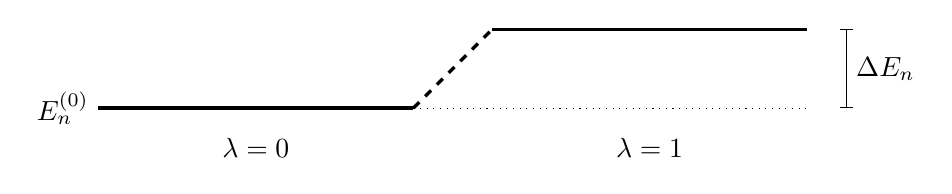
\begin{tikzpicture}
            \tikzstyle{energy level} = [very thick]
            \draw[energy level] (0, 0) -- (4, 0);
            \draw[energy level] (5, 1) -- (9, 1);
            \draw[dashed, energy level] (4, 0) -- (5, 1);
            \draw[dotted] (4, 0) -- (9, 0);
            \node[left] at (0, 0) {\(E_n^{(0)}\)};
            \draw[|-|] (9.5, 0) -- (9.5, 1);
            \node[right] at (9.5, 0.5) {\(\Delta E_n\)};
            \node at (2, -0.5) {\(\lambda = 0\)};
            \node at (7, -0.5) {\(\lambda = 1\)};
        \end{tikzpicture}
        \caption{The first order effect of a perturbation on a non-degenerate energy level of energy \(E_n^{(0)}\).}
    \end{figure}
    If instead we choose \(k \ne n\) then we have
    \[(E_k^{(0)} - E_n^{(0)})\braket{k^{(0)}}{n^{(1)}} = -\bra{k^{(0)}} \operator{H}' \ket{n^{(0)}}, \qquad k\ne n.\]
    Since \(\ket{n^{(1)}}\) is just a state it can be expanded in terms of the unperturbed eigenbasis:
    \[\ket{n^{(1)}} = \sum_{m} c_{nm}^{(1)}\ket{m^{(0)}}.\]
    Taking an inner product with \(\bra{k^{(0)}}\) we find
    \begin{align*}
        \braket{k^{(0)}}{n^{(0)}} &= \sum_m c_{nm}^{(1)}\braket{k^{(0)}}{m^{(0)}}\\
        &= \sum_{m} c_{nm}^{(1)}\delta_{km}\\
        &= c_{nk}^{(1)}.
    \end{align*}
    Hence
    \[(E_k^{(0)} - E_n^{(0)})c_{nk}^{(1)} = -\bra{k^{(0)}}\operator{H}' \ket{n^{(0)}} \implies c_{nk}^{(1)} = \frac{\bra{k^{(0)}} \operator{H'} \ket{n^{(0)}}}{E_n^{(0)} - E_k^{(0)}} = \frac{H'_{kn}}{E_n^{(0)} - E_k^{(0)}}, \qquad k \ne n.\]
    So we have now determined all of the coordinates of \(\ket{n^{(0)}}\) apart from \(c_{nn}^{(1)}\).
    However it turns out that if we choose the correction terms to be orthogonal to the unperturbed states then \(c_{nn}^{(1)} = 0\).
    Thus we have fully specified \(\ket{n^{(1)}}\) in the \(\{\ket{k^{(0)}}\}\) basis and we find that
    \[
        \tcbhighmath{\ket{n^{(1)}} = \sum_{k\ne n} \frac{\bra{k^{(0)}} \operator{H} \ket{n^{(0)}}}{E_n^{(0)} - E_k^{(0)}}\ket{k^{(0)}} = \sum_{k\ne n}\frac{H'_{kn}}{E_n^{(0)} - E_k^{(0)}}\ket{k^{(0)}}.}
    \]
    We say that the perturbation mixes the unperturbed states since the perturbed states have a small component from each unperturbed state.
    Unlike with the energy shift we have a potentially infinite sum to evaluate.
    This, along with the initial assumption that the series expansions exist, means that several things have to be `small':
    \begin{itemize}
        \item For first order changes to the eigenstate to be small we require
        \[\abs*{H'_{kn}} \ll \abs*{E_n^{(0)} - E_k^{(0)}} \forall k\ne n.\]
        \item For first order changes to the energy levels to be small we require
        \[\abs*{E_n^{(1)}} \ll \min \left\{ \abs*{E_n^{(0)}} - E_{k}^{(0)} \right\}.\]
    \end{itemize}
    Note that these conditions break down if there is degeneracy in the unperturbed system, for example some terms of the sum for \(\ket{n^{(1)}}\) will become undefined if \(E_k^{(0)} = E_n^{(0)}\) for \(k \ne n\).
    However we only need the particular energy level for the shift that we are calculating to be non-degenerate for this analysis to be correct.
    Other energy levels can be degenerate but we will need to treat them specially when we come to calculate their energy shift.
    
    \begin{example}
        \textit{Consider the potential}
        \[
            V(x) =
            \begin{cases}
                V_0\cos\left(\frac{\pi x}{2a}\right), & \abs{x} \le a,\\
                \infty, & \abs{x} > a.
            \end{cases}
        \]
        \textit{Calculate the ground state energy to first order in perturbation theory.}
        This corresponds to an infinite square well with the floor of the well bulging upwards in the centre.
        We can consider the Hamiltonian for this system to be the Hamiltonian for the square well plus a perturbative cosine term.
        We already know the solutions for the infinite square well:
        \begin{align*}
            E_n^{(0)} &= \frac{\pi^2\hbar^2n^2}{8ma^2},\\
            u_n^{(0)}(x) &= \frac{1}{\sqrt{a}}\cos\left(\frac{n\pi x}{2a}\right), \qquad n~\text{odd},\\
            u_n^{(0)}(x) &= \frac{1}{\sqrt{a}}\sin\left(\frac{n\pi x}{2a}\right), \qquad n~\text{even},\\
        \end{align*}
        The perturbation is then
        \[\operator{H}' = V_0\cos\left(\frac{\pi x}{2a}\right).\]
        This is `small' as long as \(V_0 \ll E_2^{(0)} - E_1^{(0)}\).
        The first order correction to the energy is then
        \[\Delta E = E_1^{(1)} = H'_{11} = \int_{-\infty}^{\infty} u_1^{(0)}\operator{H'}u_1^{(0)}\dd{x} = \frac{V_0}{a} \int_{-a}^{a} \cos^3\left(\frac{\pi x}{2a}\right) \dd{x} = \frac{8V_0}{3\pi} \approx 0.85V_0.\]
    \end{example}
    
    \subsection{Higher Orders}
    Sometimes the first order correction is zero.
    If this is the case then we need to go to second order.
    Going back to the result for the second order terms in \(\lambda\) we had
    \[(\operator{H}_0 - E_n^{(0)})\ket{n^{(2)}} = (E_n^{(1)} - \operator{H}')\ket{n^{(1)}} + E_n^{(2)}\ket{n^{(0)}}.\]
    Taking an inner product with an unperturbed eigenstate gives
    \[\bra{k^{(0)}}(\operator{H}_0 - E_n^{0})\ket{n^{(2)}} = \bra{k^{(0)}}(E_n^{(1)} - \operator{H}')\ket{n^{(1)}} + E_n^{(2)}\delta_{kn}.\]
    As before the first term on the left hand side can be shown to be \(E_{k}^{(0)}\braket{k^{(0)}}{n^{(2)}}\) so
    \[(E_k^{(0)} - E_{n}^{(0)})\braket{k^{(0)}}{n^{(2)}} = \bra{k^{(0)}}(E_n^{(1)} - \operator{H}')\ket{n^{(1)}} + E_n^{(2)}\delta_{kn}.\]
    In the case that \(k = n\) we find that
    \begin{align*}
        E_n^{(2)} &= \bra{n^{(0)}}\operator{H}'\ket{n^{(1)}} - E_n^{(1)}\braket{n^{(0)}}{n^{(1)}}
        \shortintertext{we choose the perturbative term \(\ket{n^{(1)}}\) to be orthogonal to the eigenstate \(\ket{n^{(0)}}\) leaving}
        &= \bra{n^{(0)}}\operator{H}'\ket{n^{(1)}}\\
        &= \sum_{m\ne n} c_{nm}^{(1)}\bra{n^0}\operator{H}'\ket{m^{(0)}}\\
        &= \sum_{m\ne n} c_{nm}^{(1)}H'_{nm}\\
        &= \sum_{m\ne n} \frac{H'_{mn}H'_{nm}}{E_n^{(0)} - E_m^{(0)}}\\
        &= \sum_{m\ne n} \frac{\abs{H'_{mn}}}{E_n^{(0)} - E_n^{(0)}}.
    \end{align*}
    Here we have used the expansion of \(\ket{n^{(1)}}\) in the \(\{\ket{m^{(0)}}\}\) eigenbasis, the formula we found for \(c_{nm}^{(1)}\), and the fact that \(H'\) is Hermitian so \(H'_{nm} = H'^*_{nm}\).
    
    We see that for the second order energy shift we have to calculate an infinite sum.
    To find the second order correction to the state we would need a double infinite sum and so on.
    Sometimes symmetry dictates that only a finite number of terms will be non-zero, sometimes we just have to truncate the sum after some number of terms.
    
    \subsection{Convergence}
    \textit{This section is non-examinable.}
    
    The series expansions that we come up with in perturbation theory often aren't actually convergent.
    This is because even though each term is small each correction contains multiple infinite sums which dominate and cause the series to diverge.
    Formally these series are asymptotic series.
    An asymptotic series for \(f\) is a series whose partial sums, that is the sum up to and including the \(n\)th term, evaluated at \(x\) can be made arbitrarily close to \(f(x)\) by taking sufficiently large \(x\).
    This differs from the usual definition of a convergent sum where the sequence of \(n\)th partial sums tends to \(f(x)\) as \(n\to\infty\) for all \(x\).
    
    \section{Degenerate, Time Independent, Perturbation Theory} 
    Suppose that the unperturbed Hamiltonian, \(\operator{H}_0\), has one eigenvalue which is \(g\)-fold degenerate.
    We label the states such that the first \(g\)-states are degenerate so
    \begin{align*}
        \operator{H}_0\ket{E_n^{(0)}} &= E^{(0)}\ket{E_n^{(0)}}, && n = 1, \dotsc, g,\\
        \operator{H}_0\ket{E_n^{(0)}} &= E_n^{(0)}\ket{E_n^{(0)}}, && n > g.
    \end{align*}
    Here \(E^{(0)}\) is the degenerate eigenvalue and \(E^{(0)} \ne E_n^{(0)}\) for \(n > g\).
    All other energy levels are non-degenerate so \(E_n^{(0)} \ne E_m^{(0)}\) for \(n\ne m\) and \(n, m > g\).
    
    We can choose a basis such that the \(g\) degenerate states are mutually orthogonal.
    Any linear combination of degenerate states, such as
    \[\ket{E^{(0)}} = \sum_{n=1}^g b_n\ket{E_n^{(0)}},\]
    will be another eigenstate of \(\operator{H}_0\) with eigenvalue \(E^{(0)}\).
    
    In the non-degenerate case we assumed that the perturbed eigenstates were close to the unperturbed states.
    More formally there was a one-to-one correspondence between the unperturbed states, \(\{n^{(0)}\}\), and the perturbed states \(\ket{n}\), and it was possible to continuously move from a perturbed state to an unperturbed state by allowing \(\lambda \to 0\).
    This cannot be assumed to be the case for a degenerate system because of the freedom we have in picking the basis for the degenerate subspace.
    In the limit \(\lambda \to 0\) we cannot be sure which of the infinite set of degenerate eigenstates the series will converge to.
    We aim to find a linear combination of eigenstates, \(\{\ket{E^{(0)}}\}\), such that these eigenstates are close to the perturbed states.
    
    As before we start with
    \[(\operator{H}_0 + \lambda\operator{H}')\ket{E} = E\ket{E}\]
    where
    \begin{align*}
        E &= E^{(0)} + \lambda E^{(1)} + \lambda^2E^{(2)} + \dotsb,\\
        \ket{E} &= \ket{E^{(0)}} + \lambda\ket{E^{(1)}} + \lambda^2\ket{E^{(2)}} + \dotsb.
    \end{align*}
    As before by equating coefficients of \(\lambda\) we see that
    \begin{align*}
        \lambda^0: && (\operator{H}_0 - E^{(0)})\ket{E^{(0)}} &= 0,\\
        \lambda^1: && (\operator{H}_0 - E^{(0)})\ket{E^{(1)}} + (\operator{H}' - E^{(1)})\ket{E^{(0)}} &= 0,\\
        \lambda^2: && (\operator{H}_0 - E^{(0)})\ket{E^{(2)}} + (\operator{H}' - E^{(1)})\ket{E^{(1)}} - E^{(2)}\ket{E^{(0)}} &= 0.
    \end{align*}
    The first of these simply restates that \(\ket{E^{(0)}}\) is an eigenstate with eigenvalue \(E^{(0)}\).
    For the second we take an inner product with the \(k\)th unperturbed state:
    \[\bra{E_k^{(0)}}(\operator{H}_0 - E^{(0)})\ket{E^{(1)}} + \bra{E_k^{(0)}}(\operator{H}' - E^{(1)})\ket{E^{(0)}}.\]
    As before we use the fact that \(\bra{E_k^{(0)}}\operator{H}_0 = E_k^{(0)}\bra{E_k^{(0)}}\) for the first term and for the second term we use
    \[\bra{E^{(0)}} = \sum_{n=1}^g b_n\ket{E_n^{(0)}}\]
    to get
    \[(E_k^{(0)} - E^{(0)})\braket{E_k^{(0)}}{E^{(0)}} + \sum_{n=1}^g b_n (H'_{kn} - E^{(1)}\delta_{kn})\]
    where
    \[H'_{kn} = \bra{E_k^{(0)}}\operator{H}'\ket{E_n^{(0)}}, \qquad\text{and}\qquad \braket{E_k^{(0)}}{E_n^{(0)}} = \delta_{kn}.\]
    We chose \(k\) arbitrarily and we now consider the case when \(k \le g\).
    In this case \(E_k^{(0)} = E^{(0)}\) so this equation reduces to
    \[\sum_{n=1}^g (H'_{kn} - E^{(1)}\delta_{kn})b_n = 0, \qquad k = 1, \dotsc, g.\]
    This is simply an eigenvalue problem in the \(g\) dimensional degenerate subspace.
    We can make this more explicit if we define a \(g\times g\) matrix, \(H'\), with components \(H'_{kn}\), and the \(g\)-dimensional identity matrix, \(\ident\), which has components \(\delta_{kn}\).
    Then this equation becomes
    \[(H' - E^{(1)}\ident)\vv{b} = 0\]
    where \(\vv{b}\) is some \(g\)-dimensional eigenvector to be determined.
    
    For this to have non-trivial solutions the determinant must be zero, so
    \[
        \begin{vmatrix}
            H'_{11} - E^{(1)} & H'_{12} & \dots & H'_{1g}\\
            H'_{21} & H'_{22} - E^{(1)} & \dots & H'_{2g}\\
            \vdots & \vdots & \ddots & \vdots\\
            H'_{g1} & H'_{g2} & \dots & H'_{gg} - E^{(1)}
        \end{vmatrix}
        = 0.
    \]
    The determinant is a \(g\) degree polynomial in \(E^{(1)}\) and therefore has \(g\) roots.
    Each root corresponds to a set of coefficients, \(\{b_n\}\).
    The roots are real since \(H'\) is a Hermitian matrix.
    There are three cases that we consider.
    \begin{itemize}
        \item \textit{All roots distinct} -- In this case the \(g\)-fold degeneracy is completely lifted at first order and the degenerate energy level splits into \(g\) distinct levels.
        \item \textit{Some roots equal} -- In this case the \(g\)-fold degeneracy is partly lifted at first order and the degenerate energy level splits into some distinct levels.
        \item \textit{All roots equal} -- In this case the degeneracy remains completely at first order, as long as the roots are non-zero there is still a first order energy shift, it just doesn't separate the energy levels.
    \end{itemize}
    These are shown in figure~\ref{fig:root possibilities}.
    \begin{figure}
        \centering
        \tikzsetnextfilename{degeneracy-breaking}
        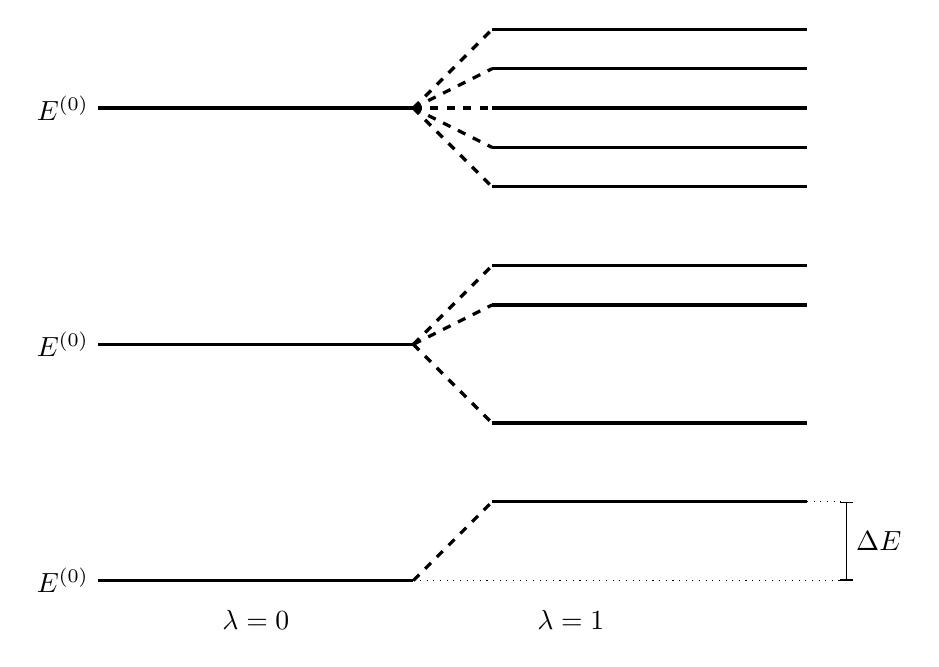
\begin{tikzpicture}
            \tikzstyle{energy level} = [very thick]
            \draw[energy level] (0, 0) -- (4, 0);
            \foreach \y in {1, 0.5, 0, -0.5, -1} {
                \draw[energy level] (5, \y) -- (9, \y);
                \draw[energy level, dashed] (4, 0)  -- (5, \y);
            }
            \node[left] at (0, 0) {\(E^{(0)}\)};
            \begin{scope}[yshift=-3cm]
                \draw[energy level] (0, 0) -- (4, 0);
                \foreach \y in {1, 0.5, -1} {
                    \draw[energy level] (5, \y) -- (9, \y);
                    \draw[energy level, dashed] (4, 0)  -- (5, \y);
                }
                \node[left] at (0, 0) {\(E^{(0)}\)};
            \end{scope}
            \begin{scope}[yshift=-6cm]
                \draw[energy level] (0, 0) -- (4, 0);
                \draw[energy level] (5, 1) -- (9, 1);
                \draw[energy level, dashed] (4, 0)  -- (5, 1);
                \node[left] at (0, 0) {\(E^{(0)}\)};
                \draw[dotted] (4, 0) -- (9.5, 0);
                \draw[dotted] (9, 1) -- (9.5, 1);
                \draw[|-|] (9.5, 0) -- (9.5, 1);
                \node[right] at (9.5, 0.5) {\(\Delta E\)};
                \node at (2, -0.5) {\(\lambda = 0\)};
                \node at (6, -0.5) {\(\lambda = 1\)};
            \end{scope}
        \end{tikzpicture}
        \caption{The three possible cases for roots of the eigenvalue problem with 5-fold degeneracy, top to bottom: all roots distinct, some roots equal, all roots equal.}
        \label{fig:root possibilities}
    \end{figure}
    \subsection{Special Cases}
    For a diagonal matrix the determinant is simply the product along the diagonal.
    If \(H'\) is diagonal then the determinant of \(H' - E^{(1)}\ident\) will be
    \[(H'_{11} - E^{(1)})(H'_{22} - E^{(1)})\dotsm(H'_{gg} - E^{(1)}) = 0\]
    which trivially has roots
    \[\Delta E_n^{(1)} = E^{(0)} = H'_{nn} = \bra{E_n^{(0)}}\operator{H}'\ket{E_n^{(0)}}, \qquad n = 1, \dotsc, g.\]
    We see that this is exactly the same as if \(\operator{H}'\) was non-degenerate.
    Normally to diagonalise a matrix we need to know the eigenvalues and eigenvectors, which requires us to solve the eigenvalue problem so doesn't actually help us solve the eigenvalue problem.
    However here we can use the compatible observables theorem to know that the matrix is diagonal without actually computing it.
    Suppose we can find an observable, \(\observable{A}\), represented by an operator, \(\operator{A}\), such that
    \[[\operator{H}_0, \operator{A}] = [\operator{H}', \operator{A}] = 0.\]
    Notice that this doesn't necessarily mean that \([\operator{H}_0, \operator{H}'] = 0\), in fact we assume this isn't the case as if it was then we wouldn't need perturbation theory.
    We use the fact that \(\operator{H}_0\) and \(\operator{A}\) have a simultaneous eigenbasis, \(\{\ket{E_n^{(0)}, A_i}\}\), and in this basis
    \begin{align*}
        \operator{H}_0\ket{E^{(0)}, A_i} &= E^{(0)}\ket{E^{(0)}, A_i}\\
        \operator{A} \ket{E^{(0)}, A_i} &= A_i \ket{E^{(0)}, A_i}.
    \end{align*}
    If the eigenvalues, \(\{A_i\}\), for \(i = 1, \dotsc, g\), are distinct then we choose these states as our basis states, that is
    \[\ket{E_n^{(0)}} = \ket{E^{(0)}, A_n}, \qquad n = 1, \dotsc, g.\]
    We then use the fact that \(\operator{H}'\) and \(\operator{A}\) commute so
    \[\bra{E_k^{(0)}}[\operator{H}', \operator{A}]\ket{E_n^{(0)}} = 0.\]
    Writing this out in full gives
    \[\bra{E_k^{(0)}}\operator{H}'\operator{A}\ket{E_n^{(0)}} - \bra{E_k^{(0)}}\operator{A}\operator{H}'\ket{E_n^{(0)}} = (A_n - A_k)\bra{E_k^{(0)}}\operator{H}'\ket{E_n^{(0)}} = (A_n - A_k)H'_{kn}.\]
    Since this must always be zero and we assume that \(A_n \ne A_k\) for \(n \ne k\) we must have that \(H'_{kn} = 0\) for \(k \ne n\).
    Thus in this eigenbasis \(\operator{H}'\) is diagonalised and so we can use the same solution as we would for the non-degenerate case.
    
    If \(A_i\) are not distinct then we look for another new operator, \(\operator{B}\), such that \(\{\operator{H}_0, \operator{A}, \operator{B}\}\) and \(\{\operator{H}', \operator{A}, \operator{B}\}\) are mutually commuting sets of operators, and so on.
    
    \begin{example}
        Consider a central potential, \(\operator{V}(r)\), along with spin 1/2 spin-orbit interaction, that is an interaction between the dipole of an electron and the magnetic field it sees due to moving in an electric field.
        The Hamiltonian for this system can be written as
        \[\operator{H} = \frac{\operator{P}^2}{2m} + \operator{V}(r) + f(r)\vecoperator{L}\cdot\vecoperator{S} = \operator{H}_0 + \operator{H'}.\]
        where \(\operator{H}' = f(r)\vecoperator{L}\cdot\vecoperator{S}\).
        Since \(\operator{H}'\) has \(\operator{L}_x\) and \(\operator{S}_x\) components we expect \([\operator{H}', \operator{L}_z] \ne 0 \ne [\operator{H}', \operator{S}_z]\).
        However we do have \([\operator{H}', \operator{J}_z] = 0\) where \(\vecoperator{J} = \vecoperator{L} + \vecoperator{S}\).
        Thus in the coupled basis, \(\ket{n, \ell, s, j, m_j}\), we can use non-degenerate perturbation theory to compute the first order energy shifts.
        Note that \([\operator{H}_0, \vecoperator{L}\cdot\vecoperator{S}] = 0\) but \([\operator{H}_0, \operator{H}']\ne 0\) due to the \(f(r)\) term in \(\operator{H}'\) and the differential operator in \(\operator{H}_0\) due to \(\operator{P}^2 = -\hbar^2\laplacian\).
    \end{example}
    
    \section{Hydrogen Fine Structure}
    As an example of a real life use of perturbation theory we consider the fine structure of hydrogen.
    This results from considering relativistic effects.
    We won't derive these but we will state and explain what they correct for.
    Recall that the unperturbed Hamiltonian for a hydrogen like atom with \(Z\) protons is
    \[\operator{H}_0 = \frac{\operator{P}^2}{2m} + \operator{V}(r), \qquad\text{where}\qquad \operator{V}(r) = -\frac{Ze^2}{4\pi\varepsilon_0r}.\]
    The eigenvalues are given by
    \[E_n^{(0)} = -\frac{m}{2\hbar^2}\left(\frac{Ze^2}{4\pi\varepsilon_0}\right)^2 \frac{1}{n^2} = -\frac{e^2}{2(4\pi\varepsilon_0)a_0}\frac{Z^2}{n^2} = -mc^2\frac{(Z\alpha)}{2n^2}\]
    where \(a_0\) is the Bohr radius and \(\alpha\) is the fine structure constant defined by
    \[a_0 = \frac{4\pi\varepsilon_0\hbar^2}{me^2}, \qquad\text{and}\qquad \alpha = \frac{e^2}{4\pi\varepsilon_0\hbar c} \approx \frac{1}{137}.\]
    One commonly used unit in this context is the rydberg unit of energy defined by
    \[\SI{1}{\rydberg} = \frac{e^2}{2(4\pi\varepsilon_0)a_0} = \SI{13.6}{\electronvolt}.\]
    The ground state of hydrogen is then \(\SI{-1}{\rydberg} = \SI{-13.6}{\electronvolt}\).
    
    \subsection{Perturbed Hamiltonian}
    The perturbation to the Hamiltonian, \(\operator{H}'\), can be further decomposed into three parts:
    \[\operator{H}' = \operator{H}'_{\mathrm{KE}} + \operator{H}'_{\mathrm{SO}} + \operator{H}'_{\mathrm{Darwin}}.\]
    The first term is a relativistic correction to the kinetic energy, which in special relativity is given by \((\gamma - 1)mc^2\).
    Expanding this we see that
    \[(\gamma - 1)mc^2 = \frac{1}{2}mv^2 + \frac{3}{8}m\frac{v^4}{c^2} + \order{v^6}.\]
    For the speeds that an electron travels this fourth order term is small but not entirely negligible.
    It leads to the perturbation
    \[\operator{H}'_{\mathrm{KE}} = -\frac{\operator{P}^4}{8m^3c^2}.\]
    
    The second term is the spin-orbit term which accounts for the interaction between the intrinsic magnetic dipole moment of the electron and the magnetic field that the electron sees due to moving in the electric field created by the nucleus.
    The form of this perturbation is
    \[\operator{H}'_{\mathrm{SO}} = f(r)\vecoperator{L}\cdot\vecoperator{S}\]
    where
    \[f(r) = \frac{2}{m^2c^2r}\dv{V}{r}.\]
    
    The third term, known as the Darwin term\footnote{Named after Charles Galton Darwin who was the grandson of Charles Robert Darwin of evolution fame.} is a relativistic correction to the potential energy given by
    \[\operator{H}'_{\mathrm{Darwin}} = \frac{\hbar^2}{8m^2c^2}\laplacian V(\vv{r}) = \frac{\pi\hbar^2}{2m^2c^2}\frac{Ze^2}{4\pi\varepsilon_0}\delta(\vv{r})\]
    where \(\delta\) is the Dirac delta distribution.
    
    \subsection{Kinetic Energy Correction}
    The unperturbed energy level \(E_n^{(0)}\) for some specific \(n\) is \(2n^2\)-fold degenerate.
    However since \(\operator{H}'_{\mathrm{KE}}\) contains no spin components we know it commutes with \(\operator{S}^2\) and \(\operator{S}_z\).
    It can also be shown that \(\operator{H}'_{\mathrm{KE}}\) commutes with \(\operator{L}^2\) and \(\operator{L}_z\).
    Therefore in the uncoupled basis, \(\{\ket{n, \ell, m_\ell, s, m_s}\}\), \(\operator{H}'_{\mathrm{KE}}\) will be diagonal.
    This means that if we work in the uncoupled basis we can use non-degenerate perturbation theory.
    Since \(\operator{H}'_{\mathrm{KE}}\) has no effect on the spin components we drop \(s\) and \(m_s\) from the notation.
    The first order energy shift is
    \begin{align*}
        \Delta E_{\mathrm{KE}} &= \bra{n, \ell, m_\ell}\left(-\frac{\operator{P}^4}{8m^3c^2}\right)\ket{n, \ell, m_\ell}\\
        &= -\frac{1}{2mc^2}\bra{n, \ell, m_\ell}\operator{T}^2\ket{n, \ell, m_\ell}.
    \end{align*}
    Here we have used the fact that
    \[\operator{T} = \frac{\operator{P}^2}{2m} \implies \operator{T}^2 = \frac{\operator{P}^4}{4m^2}.\]
    Rather than try to compute the fourth derivative, \(\laplacian\laplacian \Psi(\vv{r})\), we use the fact that \(\operator{T} = \operator{H}_0 - \operator{V}(r)\) and therefore
    \[\operator{T}^2 = \operator{H}_0^2 - \operator{H}_0\operator{V}(r) - \operator{V}(r)\operator{H}_0 + \operator{V}(r)\]
    and then \(\Delta E_{\mathrm{KE}}\) is proportional to the expectation value of this:
    \[\Delta E_{\mathrm{KE}} = -\frac{1}{2mc^2}({E_n^{(0)}}^2 - 2E_n^{(0)}\expected{\operator{V}}_{n\ell m_\ell} + \expected{\operator{V}^2}_{n\ell m_\ell}).\]
    Since \(\operator{V} \propto 1/r\) to evaluate the right hand side we simply need \(\expected{1/r}\) and \(\expected{1/r^2}\) which can be shown to be
    \[\expectedResize{\frac{1}{r}}_{n} = \frac{Z}{a_0}\frac{1}{n^2}, \qquad\text{and}\qquad \expectedResize{\frac{1}{r^2}}_{n\ell} = \frac{Z^2}{a_0^2}\frac{1}{n^3(\ell + 1/2)}.\]
    So we find that
    \[\Delta E_{\mathrm{KE}} = -E_n^{(0)}\frac{(Z\alpha)^2}{n^2}\left[\frac{3}{4} - \frac{n}{\ell + 1/2}\right].\]
    As a quick sanity check we see that this is proportional to \(\alpha^2E_n^{(0)} \approx \num{5e-5}E_n^{(0)}\) so the energy shift is indeed small compared to the size of the energy levels, \(E_n^{(0)}\).
    
    \subsection{Spin-Orbit Correction}
    For given values of \(n\) and \(\ell\) the \(E_n^{(0)}\) energy level is \(2(2\ell + 1)\)-fold degenerate.
    This is due to the \(2\ell + 1\) different values of \(m_\ell\) for each value of \(\ell\) and the two possible values of \(m_s\), i.e. \(\pm 1/2\).
    
    However if we work in the coupled basis, \(\{n,\ell, s, j, m_j\}\), then we can use non-degenerate theory.
    To see that this is valid first note that
    \[\operator{H}'_{\mathrm{SO}} = f(r)\vecoperator{L}\cdot\vecoperator{S} = \frac{1}{2}f(r)[\operator{J}^2 - \operator{L}^2 - \operator{S}^2]\]
    and
    \[[\operator{J}^2 - \operator{L}^2 - \operator{S}^2]\ket{n, \ell, s, j, m_j} = [j(j + 1) - \ell(\ell + 1) - s(s + 1)]\hbar^2\ket{n, \ell, s, j, m_j}.\]
    Since this is just an eigenvalue equation we see that \(\operator{H}'_{\mathrm{SO}}\) is diagonal in the coupled basis.
    Thus the energy shift is simply the expectation value in this basis:
    \begin{align*}
        \Delta E_{\mathrm{SO}} &= \bra{n, \ell, s, j, m_j} \operator{H}'_{\mathrm{SO}}\ket{n, \ell, s, j, m_j}\\
        &= \frac{1}{2}[j(j + 1) - \ell(\ell + 1) - s(s + 1)]\hbar^2\expected{f(r)}.
    \end{align*}
    This simplifies since we are considering an electron we know that \(s = 1/2\) and by the angular momentum addition theorem this means that for a given value of \(\ell\)  we have \(j = \ell + 1/2\) or \(j = \ell - 1/2\).
    This means that a state of given \(n\) and \(\ell\) is split into a doublet by the spin-orbit interaction.
    Since \(f(r)\) is independent of \(\vartheta\) and \(\varphi\) and of the spin the expectation value can be written as
    \[\expected{f(r)} = \frac{1}{2m^2c^2}\frac{Ze^2}{4\pi\varepsilon_0}\int_0^{\infty} \frac{1}{r^3}\abs{R_{n\ell}(r)}^2r^2\dd{r}.\]
    Note that the \(1/r^3\) comes from \(f\) and the \(r^2\) comes from the integration measure in polar coordinates.
    It can be shown that
    \[\expectedResize{\frac{1}{r^3}}_{n\ell} = \frac{Z^3}{a_0^3}\frac{1}{n^3\ell(\ell + 1/2)(\ell + 1)}.\]
    For \(\ell \ne 0\) we then find
    \[\Delta E_{\mathrm{SO}} =
        \begin{cases}
            -E_n^{(0)}\frac{(Z\alpha)^2}{2n}\frac{\ell}{\ell(\ell + 1/2)(\ell + 1)}, & j = \ell + \frac{1}{2},\\
            E_n^{(0)}\frac{(Z\alpha)^2}{2n}\frac{1}{\ell(\ell + 1/2)}, & j = \ell - \frac{1}{2}.
        \end{cases}
    \]
    
    \subsection{Darwin Correction}
    The Darwin correction is non-zero only at \(\vv{r} = \vv{0}\) as it is proportional to \(\delta(\vv{r})\).
    The radial function, \(R_{n\ell}(r)\), vanishes at the origin when \(\ell \ne 0\).
    Therefore we only need to consider this term at the origin when \(\ell = 0\) and consequently \(m_\ell = 0\).
    This term also contains no spin components so has no effect on the spin so again we drop \(s\) and \(m_s\) from the notation.
    We find that
    \begin{align*}
        \Delta E_{\mathrm{Darwin}} &= \frac{\pi\hbar^2}{2m^2c^2}\frac{Ze^2}{4\pi\varepsilon_0}\bra{n, 0, 0}\delta(\vv{r})\ket{n, 0, 0}\\
        &= \frac{\pi\hbar^2}{2m^2c^2}\frac{Ze^2}{4\pi\varepsilon_0}\int u_{n00}^*(\vv{r})\delta(\vv{r})u_{n00} \dd[3]{r}\\
        &= \frac{\pi\hbar^2}{2m^2c^2}\frac{Ze^2}{4\pi\varepsilon_0}\abs{u_{n00}(\vv{0})}^2
    \end{align*}
    where in the last step we used the sifting property of the Dirac delta distribution.
    This simplifies as
    \[\abs{u_{n00}(\vv{0})} = \abs{Y_0^0(\vartheta, \varphi)}^2\abs{R_{n\ell}(0)}^2 = \frac{1}{4\pi}\abs{R_{n\ell}(0)}^2 = \frac{Z^3}{\pi a_0^3n^3}.\]
    Hence
    \[\Delta E_{\mathrm{Darwin}} = -E_n^{(0)}\frac{(Z\alpha)^2}{n}.\]
    
    \subsection{Total Correction}
    Combining all three terms it can be shown that
    \[\Delta E_{nj} = E_n^{(0)}\frac{(Z\alpha)^2}{n^2}\left[\frac{n}{j + 1/2} - \frac{3}{4}\right].\]
    
    \begin{figure}[ht]
        \centering
        \tikzsetnextfilename{hydrogen-fine-structure}
        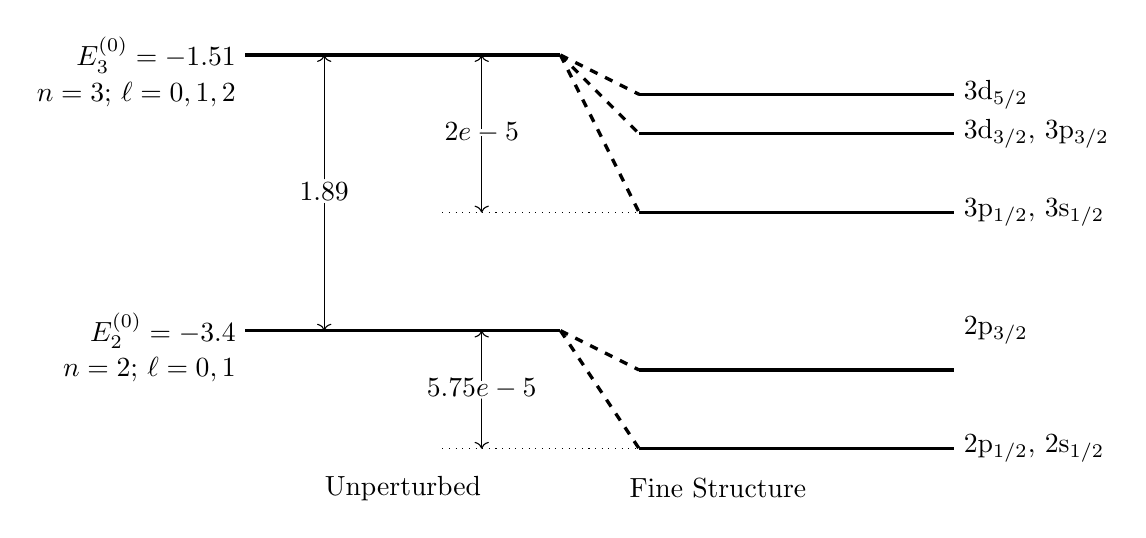
\begin{tikzpicture}
            \tikzstyle{energy level} = [very thick]
            \draw[energy level] (0, 5) -- (4, 5);
            \foreach \y in {4.5, 4, 3} {
                \draw[energy level] (5, \y) -- (9, \y);
                \draw[energy level, dashed] (4, 5) -- (5, \y);
            }
            \draw[energy level] (0, 1.5) -- (4, 1.5);
            \foreach \y in {1, 0} {
                \draw[energy level] (5, \y) -- (9, \y);
                \draw[energy level, dashed] (4, 1.5) -- (5, \y);
            }
            \node[left] at (0, 5) {\(E_3^{(0)} = \SI{-1.51}{\electronvolt}\)};
            \node[left] at (0, 1.5) {\(E_2^{(0)} = \SI{-3.4}{\electronvolt}\)};
            
            \node[right] at (9, 4.5) {\(3\mathrm{d}_{5/2}\)};
            \node[right] at (9, 4) {\(3\mathrm{d}_{3/2}\), \(3\mathrm{p}_{3/2}\)};
            \node[right] at (9, 3) {\(3\mathrm{p}_{1/2}\), \(3\mathrm{s}_{1/2}\)};
            \node[right] at (9, 1.5) {\(2\mathrm{p}_{3/2}\)};
            \node[right] at (9, 0) {\(2\mathrm{p}_{1/2}\), \(2\mathrm{s}_{1/2}\)};
            
            \contourlength{1pt}
            \contournumber{32}
            \draw[<->] (1, 5) -- (1, 1.5) node[midway] {\contour{white}{\(\SI{1.89}{\electronvolt}\)}};
            \draw[dotted] (2.5, 3) -- (5, 3);
            \draw[<->] (3, 3) -- (3, 5) node[midway] {\contour{white}{\(\SI{2e-5}{\electronvolt}\)}};
            \draw[dotted] (2.5, 0) -- (5, 0);
            \draw[<->] (3, 0) -- (3, 1.5) node[midway] {\contour{white}{\(\SI{5.75e-5}{\electronvolt}\)}};
            \node[left] at (0, 4.5) {\(n = 3\); \(\ell = 0, 1, 2\)};
            \node[left] at (0, 1) {\(n = 2\); \(\ell = 0, 1\)};
            \node at (2, -0.5) {Unperturbed};
            \node at (6, -0.5) {Fine Structure};
        \end{tikzpicture}
        \caption{The fine structure of the \(n = 2, 3\) energy levels of hydrogen (not to scale).}
        \label{fig:H fine structure}
    \end{figure}
    The resulting energy levels that occur when we account for relativistic effects are shown (not to scale) in figure~\ref{fig:H fine structure}.
    Since \(\Delta E \propto \alpha^2\) the energy shifts are therefore on the order of \(\SI{e-4}{\electronvolt}\).
    The degeneracy between the states with \(\ell = j \pm 1/2\), such as \(\termNotation[2]{}{\mathrm{p}}{1/2}\) and \(\termNotation[2]{}{\mathrm{s}}{1/2}\), is lifted if we take into account effects from \gls{qed}.
    This shift, called the Lamb shift, was discovered experimentally in 1947 by Lamb and Rutherford.
    In atomic hydrogen this shift is another two orders of magnitude smaller than the relativistic shifts, on the order of \(\SI{4e-6}{\electronvolt}\).
    
    \subsection{Term Notation}
    Term notation, also know as Russell--Saunders notation is a way of denoting a particular state with orbital angular momentum \(\ell\), spin \(s\), and total angular momentum \(j\).
    Such states are denoted
    \[\termNotation{2s + 1}{l}{j}.\]
    Here \(l\) is a letter corresponding to a particular value of \(\ell\) as given in table~\ref{tab:l letters}
    \begin{table}[ht]
        \centering
        \begin{tabular}{c|cccccccc}
            \(\ell\) & 0 & 1 & 2 & 3 & 4 & 5 & 6 & 7\\\hline
            \(l\)    & s & p & d & f & g & h & i & k
        \end{tabular}
        \caption{The orbital angular momentum quantum number, \(\ell\), and the corresponding letter used in term notation. From \(f\) onwards the letters are simply alphabetical skipping \(\mathrm{j}\). The first few letters come from the names for the corresponding spectral lines, namely sharp, primary, diffuse, and fundamental}
        \label{tab:l letters}
    \end{table}
    If the principle quantum number, \(n\), is important then it is prepended:
    \[\termNotation[n]{2s + 1}{l}{j}.\]
    Since for one electron atoms like hydrogen the spin is always \(s = 1/2\) often the spin is dropped from the notation.
    
    For example the ground state of hydrogen has \(n = 1\), \(\ell = 0\), \(s = 1/2\), and \(j = 1/2\).
    Therefore the corresponding state can be denoted as any of the following:
    \[\termNotation[1]{2}{\mathrm{s}}{1/2}, \qquad \termNotation[1]{}{\mathrm{s}}{1/2}, \qquad \termNotation{2}{\mathrm{s}}{1/2}, \qquad \termNotation{}{\mathrm{s}}{1/2} \qquad\text{or}\qquad \termNotation{}{\mathrm{s}}{}.\]
    
    \section{Helium Atom}
    \subsection{The Hamiltonian}
    Helium, \ce{He}, is the second element on the periodic table.
    It has two protons and two electrons.
    We label these electrons 1 and 2.
    The Hamiltonian for a \ce{He} atom is
    \[\operator{H} = \operator{H}_1 + \operator{H}_2 + \frac{e^2}{4\pi\varepsilon\abs{\vv{r_1} - \vv{r_2}}}\]
    where
    \[\operator{H}_i = \frac{\operator{P}_i^2}{2m} - \frac{2e^2}{4\pi\varepsilon_0}.\]
    This Hamiltonian is the sum of the a Hamiltonian for hydrogen like atom as well as an electron--electron interaction term.
    Notice that the Hamiltonian is symmetric under exchanging of the two electrons.
    That is if we change all the terms labelled 1 to be labelled 2 and vice versa the Hamiltonian wouldn't change.
    This is important as electrons are identical so it should be able to swap them without changing the physics.
    Our goal in this section is to apply perturbation theory to find the energy of the ground state.
    
    \subsection{Electron Wave Functions}
    Before we can apply perturbation theory we need to know the ground state of the unperturbed system.
    We first consider the spin components.
    Recall that since electrons are spin 1/2 particles the entire system is thus a spin 1 system.
    We will use a condensed notation where
    \[\alpha = \ket{\spinUp}, \qquad \beta = \ket{\spinDown}, \qquad \chi_{SM_S} = \ket{s_1 = 1/2, s_2 = 1/2, S, M_S}.\]
    We will also use subscripts for \(\alpha\) and \(\beta\) to denote the electron that the state corresponds to.
    As well as this tensor products will simply be written by putting the two vectors next to each other without the usual \(\tensorProd\) symbol.
    
    Recall that there are three triplet states:
    \[\chi_{11} = \alpha_1\alpha_2, \qquad \chi_{10} = \frac{1}{\sqrt{2}}[\alpha_1\beta_2 + \beta_1\alpha_2], \qquad\text{and}\qquad \chi_{1,-1} = \beta_1\beta_2,\]
    and one singlet state:
    \[\chi_{00} = \frac{1}{\sqrt{2}}[\alpha_1\beta_2 - \beta_1\alpha_2].\]
    Notice the triplet states are symmetric under exchange of the two electrons whereas the singlet state is antisymmetric.
    This is important because the spin statistics theorem tells us that the symmetry of a wave function for the whole system must be antisymmetric under exchange of the two electrons.
    That is
    \[\Psi(1, 2) = \psi(\vv{r_1}, \vv{r_2})\chi = -\Psi(2, 1).\]
    
    We start by treating neglecting the electron--electron Coulomb interaction and consider the system as two independent hydrogenic atoms with \(Z = 2\) which have a combined Hamiltonian
    \[\operator{H}_0 = \operator{H}_1 + \operator{H}_2.\]
    We already know the eigenfunctions for \(\operator{H}_i\) are
    \[\operator{H}_iu_{n_i\ell_im_{\ell_i}}(\vv{r_i}) = E_{n_i}u_{n_i\ell_im_{\ell_i}}(\vv{r_i}).\]
    Since the two Hamiltonians only act on their respective electron's:
    \[\operator{H}_iu_{n_1\ell_1m_{\ell_1}}(\vv{r_1})u_{n_2\ell_2m_{\ell_2}}(\vv{r_2}) = E_{n_i}u_{n_1\ell_1m_{\ell_1}}(\vv{r_1})u_{n_2\ell_2m_{\ell_2}}(\vv{r_2})\]
    wave function the action of the total Hamiltonian on the combined state is simply
    \begin{align*}
        \operator{H}_0 u_{n_1\ell_1m_{\ell_1}}(\vv{r_1})u_{n_2\ell_2m_{\ell_2}}(\vv{r_2}) &= (\operator{H}_1 + \operator{H}_2) u_{n_1\ell_1m_{\ell_1}}(\vv{r_1}) u_{n_2\ell_2m_{\ell_2}}(\vv{r_2})\\
        &= (E_{n_1} + E_{n_2}) u_{n_1\ell_1m_{\ell_1}}(\vv{r_1}) u_{n_2\ell_2m_{\ell_2}}(\vv{r_2})\\
        &= E_n u_{n_1\ell_1m_{\ell_1}}(\vv{r_1}) u_{n_2\ell_2m_{\ell_2}}(\vv{r_2}).
    \end{align*}
    So the energy eigenvalues are given by
    \[E_n = E_{n_1} + E_{n_2}, \qquad\text{where}\qquad E_{n_i} = -\frac{m}{2\hbar^2}\left(\frac{2e^2}{4\pi\varepsilon_0}\right)^2\frac{1}{n_i^2}.\]
    
    \subsection{Unperturbed Ground State}
    We are only interested in the ground state, that is \(n = 1\), which corresponds to both constituent systems also being in their ground states, \(n_i = 1\).
    The energy of the ground state, ignoring the effects of the perturbation, is
    \[E_{n=1} = E_{n_1=1} + E_{n_2=1} = 2E_{n_2=1}.\]
    Now we use the fact that for hydrogen with \(Z = 1\) the ground state energy is \(-\SI{13.6}{\electronvolt}\) and helium has the same form of energy levels but with \(Z = 2\).
    Since \(Z\) appears squared in the energy level we expect \(E_{n_i} = 4\cdot(-\SI{13.6}{\electronvolt})\).
    Thus the total energy of the ground state is
    \[E_n = 2\cdot 4 \cdot (-\SI{13.6}{\electronvolt}) = -\SI{108.8}{\electronvolt}.\]
    Experimentally we actually measure the ground state energy to be \(-\SI{78.957}{\electronvolt}\) which is higher.
    The reason this is higher is the repulsive force between the electrons which we have not yet considered.
    
    The wave function in the ground state has \(n_1 = n_2 = 1\) and \(\ell_1 = \ell_2 = m_{\ell_1} = m_{\ell_2} = 0\) which gives the joint spatial wave function in the ground state
    \[\psi_{\mathrm{GS}}(\vv{r_1}, \vv{r_2}) = u_{100}(\vv{r_1})u_{100}(\vv{r_2}).\]
    At this point we remark that the electronic configuration of \ce{He} is typically denoted \(\termNotation[1]{}{\mathrm{s}}{}^2\) where the 1 refers to the value of \(n\), \(s\) corresponds to \(\ell = 1\) and \(2\) tells us that there are two electrons in this state.
    Notice that the ground state wave function is symmetric under exchange of the electrons and therefore for the total ground state wave function, \(\Psi_{\mathrm{GS}} = \psi_{\mathrm{GS}}\chi_{\mathrm{GS}}\), to be antisymmetric \(\chi_{\mathrm{GS}}\) must be antisymmetric.
    Therefore we conclude that \(\chi_{\mathrm{GS}} = \chi_{00}\) as this is the only antisymmetric spin state.
    The total ground state wave function is then
    \[\ket{\Psi_{\mathrm{GS}}} \representation u_{100}(\vv{r_1})u_{100}(\vv{r_2})\chi_{00}.\]
    
    \subsection{The Perturbation}
    We are now in a position to apply perturbation theory to estimate the ground state energy.
    As usual we start with the Hamiltonian
    \[\operator{H} = \operator{H}_0 + \operator{H}'\]
    where
    \[\operator{H}_0 = \operator{H}_1 + \operator{H}_2, \qquad\text{and}\qquad \operator{H}' = \frac{e^2}{4\pi\varepsilon_0\abs{\vv{r_1}-\vv{r_2}}}.\]
    For brevity of notation let \(r_{12} = \abs{\vv{r_1} - \vv{r_2}}\).
    The first order correction to the ground state is then
    \begin{align*}
        \Delta E_1 &= \bra{\Psi_{\mathrm{GS}}} \operator{H}' \ket{\Psi_{\mathrm{GS}}}\\
        &= \bra{\psi, \chi_{00}} \operator{H}' \ket{\psi, \chi_{00}}\\
        &= (\bra{\psi}\tensorProd\bra{\chi_{00}}) \operator{H}' (\ket{\psi} \tensorProd \ket{\chi_{00}})\\
        &= \bra{\psi}\operator{H}'\ket{\psi} \tensorProd \bra{\chi_{00}} \operator{H}' \ket{\chi_{00}}\\
        &= \bra{\psi}\operator{H}'\ket{\psi} \tensorProd \braket{\chi_{00}}{\chi_{00}}\\
        &= \bra{\psi}\operator{H}'\ket{\psi}
    \end{align*}
    Here we have used the fact that \(\operator{H}'\) has no spin components and therefore doesn't act on \(\ket{\chi_{00}}\) so assuming that \(\ket{\chi_{00}}\) is properly normalised the spin terms become one and we drop them.
    Next we use the full form of the \(\termNotation[1]{}{\mathrm{s}}{}\) electron wave function:
    \[u_{100}(\vv{r}) = \frac{1}{\sqrt{\pi}} \left(\frac{Z}{a_0}\right)^{3/2}e^{-Zr/a_0}.\]
    Which gives the integral
    \[\Delta E_1 = \frac{e^2}{4\pi\varepsilon_0} \left(\frac{Z^3}{\pi a_0^3}\right)^{2} \int \frac{1}{r_{12}} \exp\left[-\frac{2Z(r_1 + r_2)}{a_0}\right] \dd[3]{r_1}\dd[3]{r_2}.\]
    This integral can then be shown to give
    \[\Delta E_1 = \frac{5}{4}Z\,\si{\rydberg} = \frac{5}{2}\,\si{\rydberg} = \SI{34}{\electronvolt}.\]
    So to first order we estimate the ground state energy to be
    \[E_1 = -\SI{108.8}{\electronvolt} + \SI{34}{\electronvolt} = -\SI{74.8}{\electronvolt} = -\SI{5.5}{\rydberg}.\]
    This is respectably close to the measured value of \(-\SI{78.957}{\electronvolt}\).
    
    One thing we do have to consider is if perturbation theory is even valid in this case.
    The perturbation is on the order of \SI{10}{\electronvolt}.
    This is only one order of magnitude smaller than the unperturbed energy which on the order of \SI{100}{\electronvolt}.
    As well as this the fine structure corrections will be on the order of \SI{10}{\electronvolt}.
    One justification for using perturbation theory is simply how close the first order energy is to the experimental value.
    
    \section{Multi-Electron Atoms}
    \subsection{Excited States of Helium}
    Recall that the Hamiltonian for Helium is
    \[\operator{H} = \operator{H_1} + \operator{H_2} + \frac{e^2}{4\pi\varepsilon_0\abs{\vv{r_1} - \vv{r_2}}}\]
    where
    \[\operator{H_i} = \frac{\operator{P}_i^2}{2m} - \frac{2e^2}{4\pi\varepsilon_0r_i}.\]
    Ignoring the electron repulsion term the first excited state for helium corresponds to exciting an electron to the first hydrogen-like excited state.
    That is one of \(n_1\) or \(n_2\) becomes \(2\) and the corresponding angular orbital momentum, \(\ell_i\) becomes 0 or 1.
    The corresponding electron configuration is then 1s2s or 1s2p with \(\ell_i = 0, 1\) respectively.
    
    Since the electrons are indistinguishable it doesn't make sense to say which electron is in the excited state.
    Instead we consider a superposition of each electron in the excited state.
    This allows us to construct the spatial wave function
    \[\psi(\vv{r_1}, \vv{r_2}) = \frac{1}{\sqrt{2}} [u_{2\ell m_\ell}(\vv{r_1})u_{100}(\vv{r_2}) \pm u_{100}(\vv{r_1})u_{2\ell m_\ell}(\vv{r_2})].\]
    This is symmetric if we choose \(+\) and antisymmetric if we choose \(-\).
    From this we can construct overall antisymmetric wave functions, the antisymmetry being dictated by spin statistics:
    \begin{align*}
        \Psi_{LM_LSM_S}^{\text{singlet}}(1, 2) &= \frac{1}{\sqrt{2}} [u_{2\ell m_\ell}(\vv{r_1})u_{100}(\vv{r_2}) + u_{100}(\vv{r_1})u_{2\ell m_\ell}(\vv{r_2})] \tensorProd \chi_{S = 0}\\
        \Psi_{LM_LSM_S}^{\text{triplet}}(1, 2) &= \frac{1}{\sqrt{2}} [u_{2\ell m_\ell}(\vv{r_1})u_{100}(\vv{r_2}) - u_{100}(\vv{r_1})u_{2\ell m_\ell}(\vv{r_2})] \tensorProd \chi_{S=1}
    \end{align*}
    Here \(L\) denotes the total angular momentum quantum number.
    It is \(0\) for the 1s2s state and 1 for the 1s2p state.
    
    We can see the degeneracy of various states by considering all possible combinations of quantum numbers allowed by the angular momentum addition theorem.
    First consider the case \(S = 0\).
    There are two options for \(L\), it can be 0 or 1.
    Recall that by the addition of angular momentum theorem the total angular momentum number, \(J\), can be any value from \(L + S\) to \(\abs{L - S}\) decreasing in integer steps.
    The degeneracy, \(g_J\), of this state is then \(2J + 1\).
    The possible values of the quantum numbers the first two excited states are given in table~\ref{tab:degeneracy of helium excited states}.
    \begin{table}[ht]
        \centering
        \begin{tabular}{c|ccc|c}
            \hline
            \(S\) & \(L\) & \(J\) & \(g_J\) &           Terms           \\ \hline
              0   &   0   &   0   &    1    & \(\termNotation{1}{S}{0}\)\\
                  &   1   &   1   &    3    & \(\termNotation{1}{P}{1}\)\\ \hline
              1   &   0   &   1   &    3    & \(\termNotation{3}{S}{1}\)\\
                  &   1   &   0   &    1    & \(\termNotation{3}{P}{0}\)\\
                  &   1   &   1   &    3    & \(\termNotation{3}{P}{1}\)\\
                  &   1   &   2   &    5    & \(\termNotation{3}{P}{2}\)\\ \hline
        \end{tabular}
        \caption{The degeneracy of the first few excited states of helium.}
        \label{tab:degeneracy of helium excited states}
    \end{table}
    We can use perturbation theory to calculate the energy shift due to the electron-electron interaction.
    The perturbation commutes with \(\operator{L}_z\) and therefore is independent of \(m_\ell\).
    This means we can calculate for a specific \(m_\ell\) and use the result for any \(m_\ell\).
    We choose \(m_\ell = 0\).
    As before the spin components commute with the perturbation and their inner product is one.
    The energy shift is then
    \begin{multline*}
        \Delta E_{\text{triplet}}^{\text{singlet}} = \frac{e^2}{2(4\pi\varepsilon_0)} \int [u_{2\ell0}(\vv{r_1})u_{100}(\vv{r_2}) \pm u_{100}(\vv{r_1})u_{2\ell0}(\vv{r_2})]^* \frac{1}{r_{12}}\\ [u_{2\ell0}(\vv{r_1})u_{100}(\vv{r_2}) \pm u_{100}(\vv{r_1})u_{2\ell0}(\vv{r_2})] \dd[3]{r_1}\dd[3]{r_2}.
    \end{multline*}
    Here \(r_{12} = \abs{\vv{r_1} - \vv{r_2}}\).
    Expanding this gives
    \begin{align*}
        \Delta E_{\text{triplet}}^{\text{singlet}} &= \frac{e^2}{2(4\pi\varepsilon_0)} \left[\int \frac{1}{r_{12}} u_{2\ell 0}^*(\vv{r_1}) u_{100}^*(\vv{r_2}) u_{2\ell0}(\vv{r_1})u_{100}(\vv{r_2}) \dd[3]{r_1}\dd[3]{r_2} \right.\\
        &\qquad\qquad\pm \int\frac{1}{r_{12}} u_{2\ell 0}^*(\vv{r_1}) u_{100}^*(\vv{r_2})u_{100}(\vv{r_1})u_{2\ell0}(\vv{r_2}) \dd[3]{r_1}\dd[3]{r_2}\\
        &\qquad\qquad\pm \int \frac{1}{r_{12}} u_{100}^*(\vv{r_1}) u_{2\ell0}^*(\vv{r_2}) u_{2\ell0}(\vv{r_1})u_{100}(\vv{r_2}) \dd[3]{r_1}\dd[3]{r_2}\\
        &\left.\qquad\qquad+ \int \frac{1}{r_{12}} u_{100}^*(\vv{r_1}) u_{2\ell0}^*(\vv{r_2}) u_{100}(\vv{r_1})u_{2\ell0}(\vv{r_2}) \dd[3]{r_1}\dd[3]{r_2}\right]\\
        &= \frac{e^2}{2(4\pi\varepsilon_0)} \left[ \int\frac{1}{r_{12}} \abs{u_{2\ell 0}(\vv{r_1})}^2\abs{u_{100}(\vv{r_2})}^2 \dd[3]{r_1}\dd[3]{r_2} \right.\\
        &\qquad\qquad\pm \int\frac{1}{r_{12}} u_{2\ell 0}^*(\vv{r_1}) u_{100}^*(\vv{r_2})u_{100}(\vv{r_1})u_{2\ell0}(\vv{r_2}) \dd[3]{r_1}\dd[3]{r_2}\\
        &\qquad\qquad\pm \int \frac{1}{r_{12}} u_{100}^*(\vv{r_1}) u_{2\ell0}^*(\vv{r_2}) u_{2\ell0}(\vv{r_1})u_{100}(\vv{r_2}) \dd[3]{r_1}\dd[3]{r_2}\\
        &\left.\qquad\qquad+ \int \frac{1}{r_{12}} \abs{u_{100}(\vv{r_1})}^2 \abs{u_{2\ell0}(\vv{r_2})}^2 \dd[3]{r_1}\dd[3]{r_2}\right]
        \shortintertext{We now use the fact that the perturbation is symmetric under exchagne of the two electrons which allows us to swap \(\vv{r_1}\) and \(\vv{r_2}\) as long as we do it for every occurence within a term}
        \Delta E_{\text{triplet}}^{\text{singlet}} &= \frac{e^2}{2(4\pi\varepsilon_0)} \left[ \int\frac{1}{r_{12}} \abs{u_{2\ell 0}(\vv{r_1})}^2\abs{u_{100}(\vv{r_2})}^2 \dd[3]{r_1}\dd[3]{r_2} \right.\\
        &\qquad\qquad\pm \int\frac{1}{r_{12}} u_{2\ell 0}^*(\vv{r_1}) u_{100}^*(\vv{r_2})u_{100}(\vv{r_1})u_{2\ell0}(\vv{r_2}) \dd[3]{r_1}\dd[3]{r_2}\\
        &\qquad\qquad\pm \int \frac{1}{r_{12}} u_{100}^*(\vv{r_2}) u_{2\ell0}^*(\vv{r_1}) u_{2\ell0}(\vv{r_2})u_{100}(\vv{r_1}) \dd[3]{r_1}\dd[3]{r_2}\\
        &\left.\qquad\qquad+ \int \frac{1}{r_{12}} \abs{u_{100}(\vv{r_2})}^2 \abs{u_{2\ell0}(\vv{r_1})}^2 \dd[3]{r_1}\dd[3]{r_2}\right]
        \shortintertext{Notice now the repeated terms which we can combine and cancel the factor of \(1/2\) in the constant at the start}
        \Delta E_{\text{triplet}}^{\text{singlet}} &= \frac{e^2}{4\pi\varepsilon_0} \left[ \int\frac{1}{r_{12}} \abs{u_{2\ell 0}(\vv{r_1})}^2\abs{u_{100}(\vv{r_2})}^2 \dd[3]{r_1}\dd[3]{r_2} \right.\\
        &\left.\qquad\qquad\pm \int\frac{1}{r_{12}} u_{2\ell 0}^*(\vv{r_1}) u_{100}^*(\vv{r_2})u_{100}(\vv{r_1})u_{2\ell0}(\vv{r_2}) \dd[3]{r_1}\dd[3]{r_2}\right]\\
    \end{align*}
    The first term looks similar to the ground state shift and is due to the interaction between the electrons.
    The second term has no classical interpretation.
    It is called the exchange contribution.
    Its sign depends on whether the total spin is 0 or 1.
    What we see is that although the perturbation doesn't depend on the spin the energy shift does as the symmetry of the wave function depends on the spin.
    
    In general the energy shift for the energy level with quantum numbers \(n\) and \(\ell\) is
    \[\Delta E_{n\ell}^{\text{singlet}} = A_{n\ell} + B_{n\ell}, \qquad\text{or}\qquad \Delta E_{n\ell}^{\text{triplet}} = A_{n\ell} - B_{n\ell}.\]
    Here \(A_{n\ell}\) represents the electron interaction and \(B_{n\ell}\) represents the exchange contribution.
    Clearly \(A_{n\ell} > 0\) and it turns out that \(B_{n\ell} > 0\) to and \(B_{n\ell} < A_{n\ell}\) so we find that
    \[\Delta_{n\ell}^{\text{triplet}} < \Delta_{n\ell}^{\text{singlet}}.\]
    This should be of no suprise to chemists as it essentially says that the p orbitals are of higher energy than the s orbitals.
    This is shown if figure~\ref{fig:helium spectrum excited states}.
    The reason for this can be seen if we look at the original spatial wave functions.
    The antisymmetric spatial wave function is zero if \(\vv{r_1} = \vv{r_2}\) and very small if they are close.
    We interpret this as the electrons being, on average, further apart in this state meaning that the repulsive effect of the electron interaction is smaller in this state and hence the energy shift is smaller.
    
    \begin{figure}[ht]
        \centering
        \tikzsetnextfilename{helium-energy-levels}
        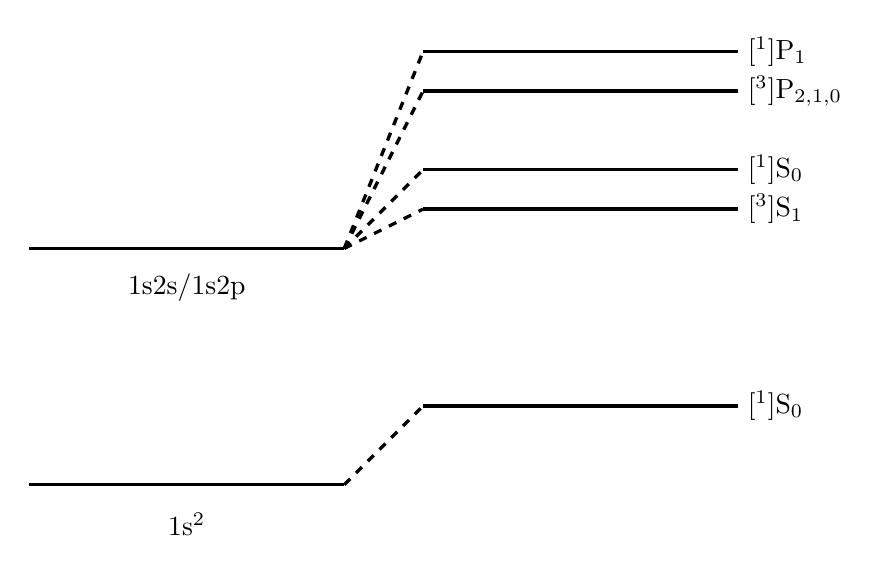
\begin{tikzpicture}
            \tikzstyle{energy level} = [very thick]
            \foreach \y in {0, 3} {
                \draw[energy level] (0, \y) -- (4, \y);
            }
            \draw[energy level] (5, 1) -- (9, 1);
            \draw[energy level, dashed] (4, 0) -- (5, 1);
            \node[right] at (9, 1) {\(\termNotation{1}{S}{0}\)};
            \foreach \y/\term in {3.5/\termNotation{3}{S}{1}, 4/\termNotation{1}{S}{0}, 5/\termNotation{3}{P}{2,1,0}, 5.5/\termNotation{1}{P}{1}} {
                \draw[energy level] (5, \y) -- (9, \y);
                \draw[energy level, dashed] (4, 3) -- (5, \y);
                \node[right] at (9, \y) {\(\term\)};
            }
            \node at (2, -0.5) {\(\mathrm{1s^2}\)};
            \node at (2, 2.5) {\(\mathrm{1s2s/1s2p}\)};
        \end{tikzpicture}
        \caption{The effect of Coulomb repulsion on the helium spectrum. Notice that this shows two possible excited states, 1s2s and 1s2p.}
        \label{fig:helium spectrum excited states}
    \end{figure}
    
    \subsection{Multi-Electron Atoms}
    Consider now a generic atom with a nuclear charge of \(Ze\) and \(N\) electrons.
    As usual we assume the nucleus is infinitely heavy and neglect all interactions apart from the Coulomb interactions.
    The Hamiltonian for this system is
    \[\operator{H} = \sum_{i=1}^{N}\left[\frac{\operator{P}_i}{2m} - \frac{Ze^2}{4\pi\varepsilon_0r_i}\right] + \sum_{i > j = 1}^{N} \frac{e^2}{4\pi\varepsilon_0 r_{ij}}.\]
    Here \(r_{ij} = \abs{\vv{r_i} - \vv{r_j}}\).
    Notice that the final sum simply sums over pairs of electrons without double counting.
    The goal is to solve the \gls{tise} but as is often the case this isn't possible so we approximate.
    
    One way of approximating is called the central field approximation.
    We treat each electron as an independent particle moving in a central potential which is a function of \(r\), the distance from the nucleus (which is assumed to be a point mass).
    The task is to come up with a potential that approximates the true potential.
    We start by considering the limiting cases of \(r \to 0\) and \(r \to \infty\).
    In the limit of \(r \to 0\) there will be no other electrons nearby and therefore we expect the only potential to be the interaction between the nucleus and electron:
    \[\lim_{r\to 0} V(r) = -\frac{Ze^2}{4\pi\varepsilon_0r}.\]
    In the limit that \(r\to\infty\) we expect all of the other \(N - 1\) electrons to be between the electron and the nucleus diluting the effective potential:
    \[\lim_{r\to\infty} V(r) = -\frac{[Z - N + 1]e^2}{4\pi\varepsilon_0 r}.\]
    Finding the intermediate form of \(V\) is not easy and is generally done by an iterative process called the Hartree--Fock method or the self-consistent field method.
    We will not discuss this here.
    
    We write the full Hamiltonian as
    \[\operator{H} = \operator{H}_c + \operator{H}'\]
    where \(\operator{H}_c\) corresponds to the central field approximation:
    \[\operator{H}_c = \sum_{i=1}^{N} \left[\frac{\operator{P}_i^2}{2m} + V(r_i)\right] = \sum_{i=1}^{N} \operator{H}_i\]
    where
    \[\operator{H}_i = \frac{\operator{P}_i^2}{2m} + V(r_i).\]
    \(\operator{H}'\) is the rest of the Hamiltonian.
    
    Considering only the central field Hamiltonian we can view it as the sum of \(N\) single particle Hamiltonians, \(\operator{H}_i\), which will have energy eigenfunctions satisfying
    \[\operator{H}_i u_{n_i\ell_im_{\ell_i}}(\vv{r_i}) = E_{n_i\ell_i}u_{n_i\ell_im_{\ell_i}}(\vv{r_i}).\]
    The energy eigenvalues are independent of \(m_{\ell_i}\) due to the spherical symmetry of \(\operator{H}_i\) but they depend on \(\ell_i\).
    The fact that the Hydrogen energy levels \emph{don't} depend on \(\ell\) turns out to be an exception rather than a rule.
    The spherical symmetry of the single particle Hamiltonians means we can decompose the energy eigenstates as
    \[u_{n_i\ell_im_{\ell_i}}(\vv{r_i}) = R_{n_i\ell_i}(r_i)Y_{\ell_i}^{m_{\ell_i}}(\vartheta_i, \varphi_i).\]
    We can then account for spin by including a spin term, \(\chi_{s_im_{s_i}}\) where, since these are single electrons \(s_i = 1/2\) and so \(m_{s_i} = \pm 1/2\).
    So the total wave function is
    \[u_{n_i\ell_im_{\ell_i}s_im_{s_i}}(i) = u_{n_i\ell_im_{\ell_i}}(\vv{r_i}) \tensorProd \chi_{s_im_{s_i}}.\]
    The total energy of the atom in this approximation is simply the sum of the individual energies:
    \[E_c = \sum_{i=1}^{N} E_{n_i\ell_i}.\]
    The wave function for the entire system is totally antisymmetric, as spin statistics demands, and is a linear combination of single electron spin orbitals given by the Slater determinant:
    \[
        \Psi(1, 2, \dotsc, N) = \frac{1}{\sqrt{N!}} 
        \begin{vmatrix}
            u_\alpha(1) & u_\beta(1) & \dotsc & u_\nu(1)\\
            u_\alpha(2) & u_\beta(2) & \dotsc & u_\nu(2)\\
            \vdots      & \vdots     & \ddots & \vdots\\
            u_\alpha(N) & u_\beta(N) & \dotsc & u_\nu(N)\\
        \end{vmatrix}
    \]
    Here \(\alpha\), \(\beta\) and \(\nu\) represent different sets of the four quantum numbers \((n, \ell, m_\ell, m_s)\) so that the final state satisfies the Pauli exclusion principle.
    
    The order of the individual energy levels doesn't depend on the potential.
    The order is
    \[\mathrm{1s2s2p3s3p[4s3d]4p[5s4d]5p[6s4f5d]}.\]
    Orbitals in square brackets are close enough in energy that the exact order can change from atom to atom.
    Electrons with the same value of \(n\) are said to be in the same shell, electrons with the same values of \(n\) and \(\ell\) are said to be in the same sub shell.
    The maximum number of electrons in the same subshell is \(2(2\ell + 1)\).
    The electron configuration of a given atom is given using a superscript to denote the number of electrons in a given subshell.
    For example in its ground state carbon has the electron configuration \(1s^22s^22p^2\) which can also be written as \([\ce{He}]\mathrm{2s^22p^2}\) where \([\ce{He}]\) denotes the electron configuration of helium in its ground state which is \(\mathrm{1s^2}\).
    
    \section{Variational Methods}
    \subsection{The Theory}
    Variational methods, also known as Rayleigh--Ritz methods, are a way of approximating the ground state energy of a given Hamiltonian, \(\operator{H}\).
    Suppose \(\operator{H}\) has a complete set of eigenstates, \(\{\ket{n}\}\), and corresponding energy eigenvalues, \(\{E_n\}\), such that \((E_n)\) is an increasing sequence, that is
    \[E_1 \le E_2 \le \dotsb \le E_{i} \le E_{i + 1} \le \dotsb\]
    Then we can expand any state, \(\ket{\psi}\), as a linear superposition of these states as
    \[\ket{\psi} = \sum_n c_n\ket{\psi}, \qquad\text{where}\qquad c_n = \braket{n}{\psi}.\]
    The expectation energy of a system in state \(\ket{\psi}\) is then
    \[\expected{E} = \frac{\bra{\psi}\operator{H}\ket{\psi}}{\braket{\psi}{\psi}} = \frac{\sum_n\abs{c_n}^2E_n}{\sum_n \abs{c_n}^2} \ge \frac{\sum_n \abs{c_n}^2 E_1}{\sum_n \abs{c_n}^2} = E_1.\]
    Where we have used the ordering of \((E_n)\) to replace all \(E_n\) with \(E_1 \le E_n\).
    We see that \(\expected{E}\) provides an upper bound for the ground state energy, \(E_1\).
    Using this fact the variational method simply gives us a way to find a close upper bound.
    
    To apply the variational method to a given Hamiltonian, \(\operator{H}\), choose a trial state, \(\ket{\psi_T}\), which depends on the parameters \(\alpha_1, \dotsc, \alpha_r\).
    We then calculate
    \[E(\alpha_1, \dotsc, \alpha_r) = \frac{\bra{\psi_T}\operator{H}\ket{\psi_T}}{\braket{\psi_T}{\psi_T}}.\]
    To find the upper bound on the ground state energy we then minimise \(E\) with respect to its parameters by finding \(\{\alpha_i^*\}\) such that
    \[\pdvat{E}{\alpha_i}{\alpha_i^*} = 0.\]
    This then gives us a best estimate for the upper bound of the ground state energy.
    
    This method works best when \(\ket{\psi_T}\) is as close to the true ground state as possible.
    This means we should consider symmetry requirements when choosing \(\ket{\psi_T}\).
    For example if our system is a particle in a box we should choose \(\psi_T(\vv{r})\) to be zero at the boundaries.
    
    It is important to note that the only thing variational methods predict is an upper bound of the ground state energy.
    The resulting trial state, \(\ket{\psi_T}\), may have a close value for the expectation value of the energy but there is no reason why it should be close to the ground state.
    Similarly if we choose our parameters, \(\{\alpha_i\}\), to have some physical meaning we shouldn't read too much into whatever values they have.
    
    \subsection{Hydrogen Ground State}
    Suppose we want to use variational methods to estimate the ground state energy of hydrogen.
    After various symmetry considerations we conclude that the ground state will have \(\ell = 0\) which means the radial part of the wave function, \(Y_\ell^m\), will be spherically symmetric.
    Thus we choose our trial solution to be the radial component of the wave function.
    Further \(\ell = 0\) is the only value where the radial component doesn't need to vanish at the origin.
    The only requirement is that our function be square integrable on \([0, \infty)\), i.e. \(\psi_T\in \squareIntegrable([0, \infty)\).
    One such function is
    \[\psi_T(r) = Ce^{-\alpha r}\]
    where \(C\) is a normalisation constant and \(\alpha\) is a variational parameter (not the fine structure coefficient).
    Notice that this is actually the form of the true wave function for the ground state.
    
    First we will normalise \(\ket{\psi_T}\) to avoid constant factors of \(1/\braket{\psi_T}{\psi_T}\).
    \begin{align*}
        \braket{\psi_T}{\psi_T} &= \int_V \psi_T^*(r)\psi_T(r) \dd{V}\\
        &= \abs{C}^2 \int_{0}^{2\pi} \dd{\varphi} \int_{0}^{\pi} \dd{\vartheta} \int_{0}^{\infty} \dd{r} e^{-2\alpha r}r^2\sin\vartheta\\
        &= \abs{C}^2\int_0^{2\pi}\dd{\varphi} \int_0^{\pi} \sin\vartheta \dd{\vartheta} \int_0^{\infty} r^2e^{-2\alpha r} \dd{r}\\
        &= \abs{C}^2\cdot2\pi\cdot 2 \cdot \left(\left[-\frac{1}{2\alpha} r^2e^{-2\alpha r}\right]_0^{\infty} + \frac{1}{\alpha}\int_0^{\infty} re^{-2\alpha r} \dd{r}\right)\\
        &= 4\pi\abs{C}^2 \frac{1}{\alpha} \int_0^{\infty} re^{-2\alpha r} \dd{r}\\
        &= 4\pi\abs{C}^2 \frac{1}{\alpha} \left(\left[-\frac{1}{2\alpha} re^{-2\alpha r}\right]_0^{\infty} + \frac{1}{2\alpha} \int_0^{\infty} e^{-2\alpha r} \dd{r}\right)\\
        &= 4\pi\abs{C}^2\frac{1}{2\alpha^2} \int_0^{\infty} e^{-2\alpha r} \dd{r}\\
        &= 4\pi\abs{C}^2\frac{1}{2\alpha^2} \left[-\frac{1}{2\alpha}e^{-\alpha r}\right]_0^{\infty}\\
        &= \pi\abs{C}^2\frac{1}{\alpha^3}
    \end{align*}
    For this to equal 1 we must have \(C = \sqrt{\alpha^3/\pi}\).
    
    The expectation value is linear so we can find \(\expected{\operator{H}}\) using
    \[\expected{\operator{H}} = \expected{\operator{T} + \operator{V}} = \expected{\operator{T}} + \expected{\operator{V}}.\]
    We will start with \(\expected{\operator{V}}\).
    \begin{align*}
        \expected{\operator{V}} &= \bra{\psi_T} \operator{V} \ket{\psi_T}\\
        &= -\frac{\abs{C}^2e^2}{4\pi\varepsilon_0} \int_V\frac{1}{r}e^{-2\alpha r} \dd{V}\\
        &= -\frac{\abs{C}^2e^2}{4\pi\varepsilon_0} \int_0^{2\pi}\dd{\varphi} \int_0^\pi \dd{\vartheta} \int_0^\infty \dd{r} \frac{1}{r}e^{-2\alpha r} r^2\sin\vartheta\\
        &= -\frac{\abs{C}^2e^2}{\varepsilon_0} \int_0^\infty re^{-2\alpha r} \dd{r}\\
        &= -\frac{\abs{C}^2e^2}{\varepsilon_0} \left(\left[-\frac{1}{2\alpha} re^{-2\alpha r}\right]_0^{\infty} + \frac{1}{2\alpha} \int_0^{\infty} e^{-2\alpha r} \dd{r} \right)\\
        &= -\frac{\abs{C}^2e^2}{\varepsilon_0} \frac{1}{2\alpha} \int_0^{\infty} e^{-2\alpha r} \dd{r}\\
        &= -\frac{\abs{C}^2e^2}{\varepsilon_0}\frac{1}{2\alpha} \left[-\frac{1}{2\alpha} e^{-2\alpha r}\right]_0^{\infty}\\
        &= -\frac{1}{4\alpha^2}\frac{\abs{C}^2e^2}{\varepsilon_0}\\
        &= -\frac{\alpha e^2}{4\pi\varepsilon_0}
    \end{align*}
    Next we find the expectation value of the energy of the kinetic energy.
    To do this we will use the following identity:
    \[\div(f \vv{v}) = f(\div\vv{v}) + (\grad f)\cdot\vv{v}.\]
    Considering the particular case \(f = \varphi^*\) and \(\vv{v} = \grad\varphi\) this becomes
    \[\div(\varphi^*\grad\varphi) = \varphi^*(\div(\grad\varphi)) + (\grad\varphi^*) \cdot (\grad\varphi).\]
    Integrating over all space this becomes
    \[\int_V \div(\varphi^*\grad\varphi) \dd{V} = \int_V \varphi^*\laplacian\varphi \dd{V} + \int_V (\grad\varphi^*)\cdot(\grad\varphi) \dd{V}.\]
    Using the divergence theorem the left hand side becomes
    \[\int_V \div(\varphi^*\grad\varphi) \dd{V} = \int_S (\varphi^*\grad\varphi)\cdot\dd{\vv{S}}.\]
    If we take \(V\) to be all of space then the boundary, \(S\), is at infinity.
    Since we are assuming \(\varphi\in\squareIntegrable(\reals^3)\) it will be zero when evaluated at infinity so the left hand side of the identity disappears and we are left with
    \[\int_V \varphi^*\laplacian\varphi \dd{V} = -\int_V \abs{\grad\varphi}^2\dd{V}.\]
    The expectation value of the the kinetic energy is then
    \begin{align*}
        \expected{\operator{T}} &= \frac{1}{2m} \bra{\psi_T} \operator{P}^2 \ket{\psi_T}\\
        &= -\frac{\hbar^2}{2m} \int_V \psi_T^* \laplacian \psi_T \dd[3]{r}\\
        &= \frac{\hbar^2}{2m} \int_V \abs{\grad\psi_T}^2\dd[3]{r}
    \end{align*}
    The trial function, \(\psi_T\), depends only on \(r\) so
    \[\grad\psi_T = \pdv{\psi_T}{r} \ve{r}\]
    and hence
    \[\abs{\grad\psi_T}^2 = \abs{\pdv{\psi_T}{r}} = \alpha^2\abs{\psi_T}^2.\]
    So
    \[\expected{\operator{T}} = \frac{\hbar^2\alpha^2}{2m}.\]
    So the expectation value of the Hamiltonian is
    \[E(\alpha) = \expected{\operator{H}} = \expected{\operator{T}} + \expected{\operator{V}} = \frac{\hbar^2\alpha^2}{2m} - \frac{e^2\alpha}{4\pi\varepsilon_0}.\]
    Differentiating with respect to \(\alpha\) we have
    \[\pdv{E}{\alpha} = \frac{\hbar^2\alpha}{m} - \frac{e^2}{4\pi\varepsilon_0}.\]
    Demanding that this is zero so \(E\) is minimised we have
    \[\alpha = \frac{me^2}{r\pi\varepsilon_0\hbar^2} = \frac{1}{a_0}\]
    where \(a_0\) is the Bohr radius.
    Thus an upper bound on the ground state energy is
    \[E = -\frac{e^2}{2(4\pi\varepsilon_0)a_0} = \SI{-1}{\rydberg} = \SI{-13.6}{\electronvolt}.\]
    This is actually the ground state energy because our trial function with \(\alpha = 1/a_0\) is the ground state eigenfunction so \(\expected{\operator{H}}\) is simply the expectation value of the energy of a particle in a ground state, which is the ground state energy.
    
    \subsection{Helium Ground State}
    Suppose we want to use variational methods to calculate the ground state energy of helium.
    As a trial wave function we take a product of 1s orbital wave functions with an effective nuclear charge \(\tilde{Z}\) which accounts for shielding of the nucleus by the other electron.
    \[\psi_T(r_1, r_2) = \frac{\tilde{Z}^3}{\pi a_0^3} \exp\left[-\frac{\tilde{Z}}{a_0}(r_1 + r_2)\right].\]
    Setting \(\tilde{Z} = Z\) would be the equivalent of no electron-electron interaction.
    The variational parameter in this wave function is \(\tilde{Z}\).
    
    For the kinetic energy we can use the same result as for hydrogen:
    \[\expected{\operator{T}} = -\frac{\hbar^2}{2m}\ket{\psi_T}(\operator{P}_1^2 + \operator{P}_2^2)\ket{\psi_T} = \frac{\hbar^2 \tilde{Z}^2}{ma_0^2} = 2\tilde{Z}^2\,\si{\rydberg}.\]
    Similarly for the potential energy
    \[\expected{\operator{V}} = -\frac{2Ze^2}{4\pi\varepsilon_0a_0} \tilde{Z} = -4Z\tilde{Z}\,\si{\rydberg}.\]
    Finally the electron-electron Coulomb term has an expectation value of \(5/4\tilde\,\si{\rydberg}\).
    The total energy is then
    \[E(\tilde{Z}) = 2\left[\tilde{Z}^2 - \left(2Z - \frac{5}{8}\right)\tilde{Z}\right] \,\si{\rydberg}.\]
    Differentiating with respect to \(\tilde{Z}\), setting equal to zero, and then rearranging gives us
    \[\tilde{Z} = Z - \frac{5}{16}.\]
    The energy corresponding to this is then
    \[E(\tilde{Z}) = \SI{-5.695}{\rydberg} = \SI{-77.46}{\electronvolt}.\]
    This is within \SI{2}{\percent} of the measured value of \(\SI{-78.975}{\electronvolt}\) and is better than the first order perturbation result of \(\SI{-74.8}{\electronvolt}\).
    
    \subsection{Excited States}
    It is sometimes possible to use variational methods to find upper bounds on excited states.
    Suppose we know enough about the ground state to choose a trial state that is orthogonal to the ground state such that \(\braket{n=1}{\psi_T} = 0\).
    Then the expansion of \(\ket{\psi_T}\) in \(\{\ket{n}\}\) doesn't contain \(\ket{n=1}\) and so
    \[\frac{\bra{\psi_T}\operator{H}\ket{\psi_T}}{\braket{\psi_T}{\psi_T}} = \frac{\sum_{n=2}\abs{c_n}^2E_n}{\sum_{n=2} \abs{c_n}^2} \ge E_2.\]
    Using variational methods as before we can then find an upper bound on \(E_2\).
    
    The problem with this is we don't typically know the eigenstates so we can't construct an orthogonal state.
    We can avoid this problem if we are interested in an excited state with symmetries lower energy states don't posses.
    If we choose a trial state that does have these symmetries then it is guaranteed to be orthogonal to the lower energy states and we can use variational methods.
    
    Consider, for example, helium.
    It's ground state is a \(\termNotation{1}{S}{}\) state.
    The first four excited states are \(\termNotation{3}{S}{}\), \(\termNotation{1}{S}{}\), \(\termNotation{3}{P}{}\), and \(\termNotation{1}{P}{}\) states/
    Apart from the \(\termNotation{1}{S}{}\) state these all have symmetries different from the ground state.
    For example \(\termNotation{}{P}{}\) states have \(L = 1\) and are therefore orthogonal to the ground state which has \(L = 0\).
    A trial function that may be considered when trying to find an upper bound on the state 1s2p is
    \[\psi_T^{\pm}(\vv{r_1}, \vv{r_2}) = C_{\pm} [f(r_1)g(r_2)\cos\vartheta_1 \pm f(r_2)g(r_2)\cos\vartheta_2]\]
    where
    \[f(r) = e^{-\alpha r / a_0}, \qquad\text{and}\qquad g(r) = re^{-\beta r/ 2a_0}.\]
    This has two variational parameters \(\alpha\) and \(\beta\).
    
        \part{Applications of Quantum Theory}
    \section{Hidden Variables, EPR Paradox and Bell's Inequality}
    \subsection{Hidden Variables}
    For most of the time up until this point we haven't thought too hard about what anything that we are doing actually means.
    We started by stating that the state of a system is specified by its wave function.
    We then went on to say that observables don't have definite values until we measure them.
    The most we can predict in general is the probability of a given result.
    This assumes (correctly) that there is no pre-existing value of the observable.
    This upset a lot of important physicists in early quantum theory, including Einstein who famously said `God does not play dice'.
    
    Einstein believed that there was an underlying reality in which observables have definite values and we are simply ignorant of this deeper reality.
    This idea, called a hidden variables theory, is similar to the assumption that, given infinite computing power, we could deterministically calculate the future of any system and wouldn't have to resort to statistical mechanics.
    While it turns out that hidden variables theories are wrong in showing so we develop several key ideas.
    
    \subsection{EPR Paradox}
    \subsubsection{Background}
    Recall that for a spin 1/2 system when measuring spin along the \(z\)-axis we can get either \(\pm 1/2\).
    This idea is the basis for the Stern--Gerlach experiment.
    The details of how aren't important here but a Stern--Gerlach experiment splits a beam of particles into two beams according to the spin along a given axis.
    For example, figure~\ref{fig:stern-gerlach z} shows a Stern--Gerlach magnet splitting a beam according to its spin along the \(z\)-axis.
    \begin{figure}[ht]
        \centering
        \tikzsetnextfilename{stern-gerlach}
        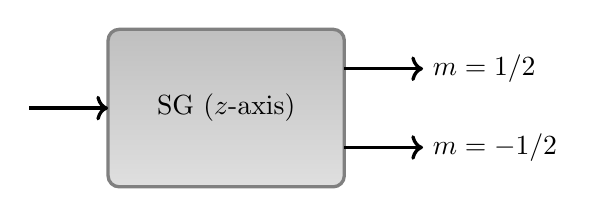
\begin{tikzpicture}
            \tikzstyle{experiment} = [draw=gray, very thick, fill=lightgray, rounded corners, top color=lightgray, bottom color=lightgray!50]
            \tikzstyle{beam} = [very thick]
            \shadedraw[experiment] (0, 0) rectangle (3, 2);
            \node at (1.5, 1) {SG (\(z\)-axis)};
            \draw[beam, ->] (-1, 1) -- (0, 1);
            \draw[beam, ->] (3, 1.5) -- (4, 1.5);
            \draw[beam, ->] (3, 0.5) -- (4, 0.5);
            \node[right] at (4, 1.5) {\(m = 1/2\)};
            \node[right] at (4, 0.5) {\(m = -1/2\)};
        \end{tikzpicture}
        \caption{Stern--Gerlach experiment splits a beam according to the spin along the \(z\)-axis.}
        \label{fig:stern-gerlach z}
    \end{figure}
    The two beams leaving this machine correspond to the two eigenstates of \(\operator{S}_z\).
    Recall that \(\operator{S}_z\) can be represented as
    \[
        \operator{S}_z \representation \frac{1}{2}\hbar
        \begin{pmatrix}
            1 & 0\\
            0 & -1
        \end{pmatrix}
        .
    \]
    This has two eigenvectors which have the following representations
    \[
        \ket{m = 1/2} \representation 
        \begin{pmatrix}
            1 \\ 0
        \end{pmatrix}
        , \qquad\text{and}\qquad \ket{m = -1/2} \representation 
        \begin{pmatrix}
            0 \\ 1
        \end{pmatrix}
        .
    \]
    It is equally valid to have a Stern--Gerlach experiment measure along the \(x\)-axis.
    The corresponding operator, \(\operator{S}_x\), has the representation
    \[
        \operator{S}_x \representation \frac{1}{2}\hbar
        \begin{pmatrix}
            0 & 1\\
            1 & 0
        \end{pmatrix}
        .
    \]
    This has two eigenvectors which have the following representations
    \[
        \ket{m_x = 1/2} \representation \frac{1}{\sqrt{2}}
        \begin{pmatrix}
            1 \\ 1
        \end{pmatrix}
        ,\qquad\text{and}\qquad \ket{m_x = -1/2} \representation \frac{1}{\sqrt{2}}
        \begin{pmatrix}
            1 \\ -1
        \end{pmatrix}
        .
    \]
    These can be written as a linear combination of eigenstates of \(\operator{S}_z\):
    \begin{align*}
        \frac{1}{\sqrt{2}} 
        \begin{pmatrix}
            1 \\ 1
        \end{pmatrix}
        &= \frac{1}{\sqrt{2}}
        \begin{pmatrix}
            1 \\ 0
        \end{pmatrix}
        + \frac{1}{\sqrt{2}}
        \begin{pmatrix}
            0 \\ 1
        \end{pmatrix}
        ,\\
        \frac{1}{\sqrt{2}} 
        \begin{pmatrix}
            1 \\ -1
        \end{pmatrix}
        &= \frac{1}{\sqrt{2}}
        \begin{pmatrix}
            1 \\ 0
        \end{pmatrix}
        - \frac{1}{\sqrt{2}}
        \begin{pmatrix}
            0 \\ 1
        \end{pmatrix}
        .
    \end{align*}
    Using a Stern--Gerlach magnet oriented in the \(x\) direction we can select the beam containing only particles in the \(\ket{m_x = -1/2}\) state.
    If we then use a second Stern--Gerlach magnet to measure the \(z\) component of the spin then we find that the probability of measuring \(m = 1/2\) is \(\abs{1/\sqrt{2}}^2 = 1/2\).
    This is shown in figure~\ref{fig:stern-gerlach x then z}
    \begin{figure}[ht]
        \centering
        \tikzsetnextfilename{double-stern-gerlach}
        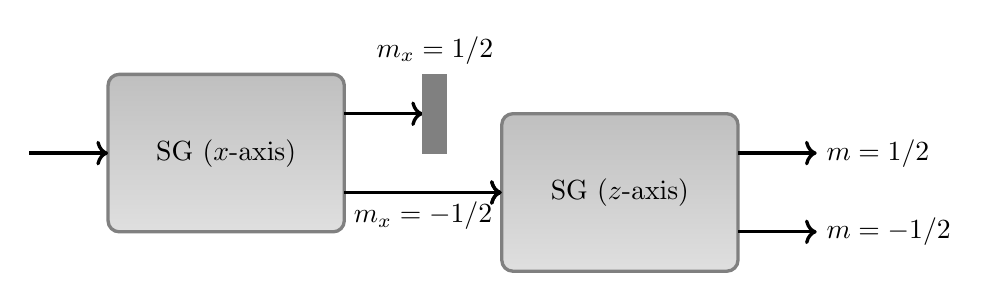
\begin{tikzpicture}
            \tikzstyle{experiment} = [draw=gray, very thick, fill=lightgray, rounded corners, top color=lightgray, bottom color=lightgray!50]
            \tikzstyle{block} = [fill=gray, color=gray]
            \tikzstyle{beam} = [very thick]
            \shadedraw[experiment] (0, 0) rectangle (3, 2);
            \node at (1.5, 1) {SG (\(x\)-axis)};
            \draw[beam, ->] (-1, 1) -- (0, 1);
            \draw[beam, ->] (3, 1.5) -- (4, 1.5);
            \draw[beam, ->] (3, 0.5) -- (5, 0.5);
            \draw[block] (4, 1) rectangle (4.3, 2);
            \node[below] at (4, 0.5) {\(m_x = -1/2\)};
            \node[above] at (4.15, 2) {\(m_x = 1/2\)};
            \begin{scope}[xshift=5cm, yshift=-0.5cm]
                \shadedraw[experiment] (0, 0) rectangle (3, 2);
                \node at (1.5, 1) {SG (\(z\)-axis)};
                \draw[beam, ->] (-1, 1) -- (0, 1);
                \draw[beam, ->] (3, 1.5) -- (4, 1.5);
                \draw[beam, ->] (3, 0.5) -- (4, 0.5);
                \node[right] at (4, 1.5) {\(m = 1/2\)};
                \node[right] at (4, 0.5) {\(m = -1/2\)};
            \end{scope}
        \end{tikzpicture}
        \caption{Stern--Gerlach experiment splits a beam according to the spin along the \(z\)-axis.}
        \label{fig:stern-gerlach x then z}
    \end{figure}
    We can more generally measure the spin along some unit vector in the \((x, z)\)-plane, \(\vh{n} = (\sin\vartheta, 0, \cos\vartheta)\).
    The corresponding operator for this measurement is
    \[
        \vecoperator{S}\cdot\vh{n} = \operator{S}_x\sin\vartheta + \operator{S}_z\cos\vartheta \representation \frac{1}{2}
        \begin{pmatrix}
            \cos\vartheta & \sin\vartheta\\
            \sin\vartheta & -\cos\vartheta
        \end{pmatrix}
        .
    \]
    This has eigenvectors
    \[
        \ket{m_{\vartheta} = 1/2} \representation
        \begin{pmatrix}
            \cos \frac{\vartheta}{2}\\
            \sin \frac{\vartheta}{2}
        \end{pmatrix}
        , \qquad\text{and}\qquad
        \ket{m_{\vartheta} = -1/2} \representation
        \begin{pmatrix}
            \sin \frac{\vartheta}{2}\\
            \cos \frac{\vartheta}{2}
        \end{pmatrix}
        .
    \]
    
    \subsubsection{The EPR Thought Experiment}
    In 1935 Einstein, Podolsky, and Rosen published a paper discussing a thought experiment that they thought demonstrated something was missing from quantum mechanics.
    We will discuss this thought experiment, known as the \gls{epr} paradox here.
    
    Consider a process where a particle with no spin decays into a pair of spin 1/2 particles, for example a photon could produce an electron-positron pair.
    To conserve momentum these particles will go off in opposite directions from the point where they were created.
    Suppose that we analyse the two particles with Stern--Gerlach magnets, \(A\) and \(B\), which can be orientated in an arbitrary direction.
    We will place \(A\) and \(B\) sufficiently far apart such that within the time taken for the experiment to occur even light cannot get between from \(A\) to \(B\).
    This means that no information can be shared during the experiment.
    This is shown in figure~\ref{fig:epr setup}.
    \begin{figure}[ht]
        \centering
        \tikzsetnextfilename{epr-setup}
        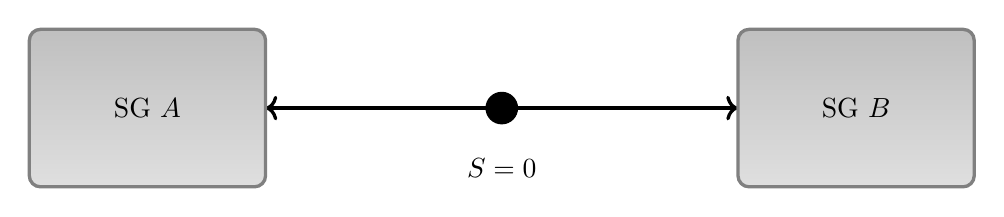
\begin{tikzpicture}
            \tikzstyle{experiment} = [draw=gray, very thick, fill=lightgray, rounded corners, top color=lightgray, bottom color=lightgray!50]
            \tikzstyle{beam} = [very thick]
            \draw[beam, <->] (-3, 1) -- (3, 1);
            \shadedraw[experiment] (3, 0) rectangle (6, 2);
            \shadedraw[experiment] (-3, 0) rectangle (-6, 2);
            \node at (4.5, 1) {SG \(B\)};
            \node at (-4.5, 1) {SG \(A\)};
            \draw[fill=black] (0, 1) circle[radius=0.2cm];
            \node[above] (0, 1) {\(S = 0\)};
        \end{tikzpicture}
        \caption{The setup for the \gls{epr} paradox.}
        \label{fig:epr setup}
    \end{figure}
    Suppose that both experiments are aligned to measure the spin along the \(z\)-axis.
    Conservation of angular momentum means that since we started with \(S = 0\) we must have \(S = 0\) at all times.
    The only way for this to happen is if the two particles have equal and opposite spins along the \(z\)-axis.
    Therefore if we measure the spin at \(A\) and get \(\hbar/2\) we know for a fact that at \(B\) they must measure \(-\hbar/2\).
    At first this seems to be the same as classical mechanics which also has conservation of angular momentum.
    However in quantum mechanics the spin isn't defined until we take a measurement.
    This means that when we make the measurement at \(A\) before the measurement the spin is undefined at both \(A\) and \(B\).
    After the measurement the spin is defined at both \(A\) and \(B\).
    Therefore by making a measurement at \(A\) we necessarily change something at \(B\).
    This raises two questions:
    \begin{enumerate}
        \item Is the fact that the outcome at \(B\) is entirely predictable a consequence of the measurement at \(A\)?
        \item If so how does the information about the measurement at \(A\) get to \(B\)?
    \end{enumerate}
    Suppose instead we had \(A\) measuring along the \(x\)-axis and \(B\) measuring along the \(z\)-axis.
    Then the measurement at \(A\) doesn't affect the outcome of the experiment at \(B\) as both of \(\ket{m_x=\pm1/2}\) are a superposition of equal parts of \(\ket{m = \pm1/2}\).
    Suppose instead that \(B\) measures at an angle \(\vartheta\) to the \(z\)-axis in the \((x, z)\)-plane.
    If \(A\) measured \(-\hbar/2\) as the \(x\) spin then we know that the particle at \(B\) must have an \(x\) component of \(\hbar/2\).
    We can then decompose the \(\hbar/2\) state along the \(z\)-axis in terms of the spin along the \(\vartheta\)-axis:
    \begin{align*}
        \begin{pmatrix}
            1\\ 0
        \end{pmatrix}
        &= \cos\frac{\vartheta}{2}
        \begin{pmatrix}
            \cos\frac{\vartheta}{2}\\\sin\frac{\vartheta}{2}
        \end{pmatrix}
        + \sin\frac{\vartheta}{2}
        \begin{pmatrix}
            \sin\frac{\vartheta}{2}\\
            -\cos\frac{\vartheta}{2}
        \end{pmatrix}
        \\
        &= \cos\frac{\vartheta}{2} \ket{m_{\vartheta} = 1/2} + \sin\frac{\vartheta}{2} \ket{m_{\vartheta} = -1/2}.
    \end{align*}
    So measuring along the \(\vartheta\)-axis \(B\) measures spin-up with probability \(\cos^2(\vartheta/2)\) and spin down with probability \(\sin^2(\vartheta/2)\).
    The measurement at \(B\) is still affected by the measurement at \(A\).
    
    The fact that measurement at \(A\) seems to affect measurements at \(B\) regardless of how far apart the two experiments are seems to imply action at a distance or faster than light information transmission.
    The solution that \gls{epr} suggested was that the particles knew before hand (or rather some hidden variables fixed before hand) the spin they would have when measured along any axis.
    However this was shown to be false by John Bell.
    
    \subsection{Bell's Inequality}
    Bell sought to the following question:
    \begin{enumerate}
        \item Is quantum mechanics a realistic local theory?
        \item If not can we make a prediction or observation that can demonstrate this.
    \end{enumerate}
    To answer these he came up with the Bell inequality.
    
    We start with the same setup as with the \gls{epr} paradox.
    We define three co-planar directions, \(\{\vh{n}\vv{_{i}}\}\), along which we can measure the spin.
    
    \subsubsection{Realistic Theory}
    In a realistic local theory the spin 1/2 particles must individually have definite values, \(\pm\hbar/2\), for each direction we can measure.
    Notice that we don't require measurement of all three directions simultaneously, this can't be done as generally spin operators along different axes don't commute.
    We will denote the two possible outcomes along a given axis by \(+\) and \(-\).
    The spin state of a particle can then be denoted \((\pm, \pm, \pm)\) where, for example, \((+, -, +)\) denotes a particle that will have spin \(\hbar/2\) if measured along \(\vh{n}\vv{_1}\) or \(\vh{n}\vv{_3}\) and \(-\hbar/2\) if measured along \(\vh{n}\vv{_2}\).
    We can denote the spin state of the whole system as \((\pm, \pm, \pm, \pm, \pm, \pm)\) which is simply the state of one particle written immediately after the state of the other particle.
    A generic state can then be written as \((\sigma_1, \sigma_2, \sigma_3, \tau_1, \tau_2, \tau_3)\) where \(\sigma_i\) and \(\tau_i\) represent the spin of the particle at \(A\) and \(B\) respectively when measured along \(\vh{n_i}\).
    We denote by \(f(\sigma_1, \sigma_2, \sigma_3, \tau_1, \tau_2, \tau_3)\) the fraction of particle pairs that are in the state \((\sigma_1, \sigma_2, \sigma_3, \tau_1, \tau_2, \tau_3)\).
    Since ew assume that the net spin is \(0\) we have \(f(\sigma_1, \sigma_2, \sigma_3, \tau_1, \tau_2, \tau_3) = 0\) unless \(\sigma_i = -\tau_i\) for all \(i\).
    This satisfies locality as we can set \(\sigma_i\) and \(\tau_i\) when the particles are first produced and close and then nothing changes when we make a measurement.
    
    \subsubsection{Spin Correlations}
    Denote by \(P_{++}(\vh{n}\vv{_i}, \vh{n}\vv{_j})\) the probability that when measuring along \(\vh{n}\vv{_i}\) (\(\vh{n}\vv{_j}\)) at \(A\) (\(B\)) we get \(+\) (\(+\)).
    Then, for example
    \begin{align*}
        P_{++}(\vh{n}\vv{_1}, \vh{n}\vv{_2}) &= \sum_{\sigma_2, \sigma_3} \sum_{\tau_1, \tau_2} f(+, \sigma_2, \sigma_3, \tau_1, +, \tau_3)\\
        &= f(+, -, +, -, +, -) + f(+, -, -, -, +, +)
    \end{align*}
    where we have used the fact that \(f\) is zero unless \(\sigma_i = -\tau_i\),
    Similarly we have
    \begin{align*}
        P_{++}(\vh{n}\vv{_3}, \vh{n}\vv{_2}) &= f(+, -, +, -, +, -) + f(-, -, +, +, +, -),\\
        P_{++}(\vh{n}\vv{_1}, \vh{n}\vv{_3}) &= f(+, +, -, -, -, +) + f(+, -, -, -, +, +).
    \end{align*}
    Since \(f\) are all non-negative we can add these last two results and we get
    \[P_{++}(\vh{n}\vv{_1}, \vh{n}\vv{_2}) \le P_{++}(\vh{n}\vv{_3}, \vh{n}\vv{_2}) + P_{++}(\vh{n}\vv{_1}, \vh{n}\vv{_3}).\]
    
    \subsubsection{Non-Realistic Theory}
    We can now compute the spin correlations that we get from quantum mechanics.
    Suppose \(\vh{n}\vv{_1}\) corresponds to the \(z\)-axis and at \(B\) we choose to measure the spin along the \(\vh{n}\vv{_2}\) direction which is at an angle \(\vartheta\) to the \(z\)-axis.
    If \(\vartheta_{ij}\) is the angle between \(\vh{n}\vv{_i}\) and \(\vh{n}\vv{_j}\) then
    \[P_{++}(\vh{n}\vv{_i}\vh{n}\vv{_j}) = \frac{1}{2}\sin^2\frac{\vartheta_{ij}}{2}, \qquad\text{and}\qquad P_{-+}(\vh{n}\vv{_i}, \vh{n}\vv{_j}) = \frac{1}{2}\cos^2\frac{\vartheta_{ij}}{2}.\]
    If Bell's inequality is to be satisfied then we must have
    \[\sin^2\frac{\vartheta_{12}}{2} \le \sin^2\frac{\vartheta_{23}}{2} + \sin^2\frac{\vartheta_{13}}{2}.\]
    Consider the case that
    \[\vartheta_{13} = \vartheta_{23} = \frac{\vartheta_{12}}{2}.\]
    Then Bell's inequality becomes
    \[\sin^2\vartheta_{13} \le 2\sin^2\frac{\vartheta_{13}}{2}.\]
    This simplifies to
    \[\cos^2\frac{\vartheta_{13}}{2} \le \frac{1}{2}.\]
    This is not satisfied if \(0 \le \vartheta_{13} \le \pi/2\).
    So if quantum mechanics is correct we would expect Bell's inequality to be violated showing it is not a realistic local theory.
    
    \subsubsection{Experimental Tests of Bell's Inequality}
    Now that we know Bell's inequality can differentiate between a realistic local theory and a non-realistic local theory we need to test to see if Bell's theory is ever violated.
    This was first done not with spins but with linearly polarised photons.
    Photons where polarised at \(A\) and \(B\) in directions \(\vh{n}\vv{_i}\) and \(\vh{n}\vv{_j}\) respectively.
    We define a result to be \(+\) when the polarisation is parallel to \(\vh{n}\vv{_i}\) and \(-\) if it is perpendicular.
    The correlation coefficient is defined as
    \[E(\vh{n}\vv{_i}, \vh{n}\vv{_j}) = P_{++}(\vh{n}\vv{_i}, \vh{n}\vv{_j}) + P_{--}(\vh{n}\vv{_i}, \vh{n}\vv{_j}) - P_{-+}(\vh{n}\vv{_i}, \vh{n}\vv{_j}) - P_{+-}(\vh{n}\vv{_i}, \vh{n}\vv{_j}).\]
    This is the expectation value in the singlet state:
    \[\expected{(\vv{\sigma\cdot\vh{n}\vv{_i}})(\vv{\sigma}\cdot\vh{n}\vv{_j})} = \cos\vartheta_{ij}.\]
    In the original experiment the combination
    \[S = E(\vh{n}\vv{_i}, \vh{n}\vv{_j}) - E(\vh{n}\vv{_i}, \vh{n}\vv{'_j}) + E(\vh{n}\vv{'_i}, \vh{n}\vv{_j}) + E(\vh{n}\vv{'_i}, \vh{n}\vv{'_j}).\]
    Where \(\vh{n}\vv{_i}\), \(\vh{n}\vv{'_i}\) and \(\vh{n}\vv{_j}\), \(\vh{n}\vv{'_j}\) represent two different orientations of the polarises at \(A\) and \(B\) respectively.
    
    In a realistic local theory a Bell inequality for this quantity is
    \[-2 \le S \le 2.\]
    Quantum mechanics on the other hand predicts
    \[-2\sqrt{2} \le S \le 2\sqrt{2}.\]
    Orientations where chosen such that
    \[\vh{n}\vv{_i}\cdot\vh{n}\vv{_j} = \vh{n}\vv{'_i}\cdot\vh{n}\vv{_j} = \vh{n}\vv{'_i}\cdot\vh{n}\vv{'_j} = \cos\varphi, \qquad\text{and}\qquad \vh{n}\vv{_i}\cdot\vh{n}\vv{'_j} = \cos3\varphi.\]
    The value of \(S\) was then determined for various values of \(\varphi\) between \(0^\circ\) and \(90^\circ\).
    The results violated Bell's inequality.
    The maximum violation was at \(\varphi = 22.5^\circ\) where they measured \(S = 2.697 \pm 0.015\).
    
    \section{Quantum Teleportation}
    In the last section we introduced the idea of entangled particles.
    These can be used in many different ways to do things that can't be done classically.
    The first use we will consider is quantum teleportation.
    This allows for information about one quantum state to be transferred to another location.
    No matter is transferred, only information.
    This process is called teleportation because if a second particle is placed into the same state that is sent to the remote location then it as if the particle teleported.
    The process requires both quantum and classical communication and the restriction of the classical communication to be slower than the speed of light means that information cannot be transferred faster than the speed of light.
    
    \subsection{Entanglement}
    In classical computing the most basic unit of information is the bit which can be either 0 or 1.
    In quantum computing the most basic unit of information is the \define{qubit} which is a two state system, which can be described by the Hilbert space \(\hilbert_\text{qubit}\).
    Often we identify one state with 0 and the other with 1.
    As a matter of notation in this section we will refer to two states, \(\ket{+}\) and \(\ket{-}\) although later on we will refer to the same two states as \(\ket{0}\) and \(\ket{1}\) respectively in a different context.
    We will often think of the states as electron spins, for example we may identify spin up with \(\ket{+}\) and spin down with \(\ket{-}\).
    We choose electron spins simply because we are familiar with the mathematics behind them but in practice any two state system could be used.
    In this case it is natural to make the following identification with spinor states:
    \[
        \ket{+} \representation 
        \begin{pmatrix}
            1\\ 0
        \end{pmatrix}
        , \qquad\text{and}\qquad
        \begin{pmatrix}
            0\\ 1
        \end{pmatrix}
        .
    \]
    The main difference from a classical bit is that a qubit is in a quantum superposition of the two pure states.
    A generic qubit state, \(\ket{\psi}\in\hilbert_{\text{qubit}}\), is then
    \[\ket{\psi} = a_-\ket{-} + a_+\ket{+}\]
    for some \(a_-, a_+\in\complex\) such that \(\abs{a_-}^2 + \abs{a_+}^2 = 1\).
    We can parametrise this as
    \[\ket{\psi} = \cos\frac{\vartheta}{2}\ket{+} + e^{i\varphi}\sin\frac{\vartheta}{2}\ket{-}\]
    where \(\vartheta\in[0, \pi]\) and \(\varphi\in[0, 2\pi]\).
    We are free to choose the phase of \(\ket{\psi}\) to make \(a_-\) real.
    When we do this we often represent the state as a point on the Bloch sphere as shown in figure~\ref{fig:bloch sphere 2}.
    \tikzexternaldisable
    \begin{figure}[ht]
        \centering
        \tikzsetnextfilename{bloch-sphere-qubits}
            \begin{blochsphere}[nested=false, radius=3cm, ball=3d]
                \drawBall[radius=3cm, opacity=0.2];
                \drawBallGrid[radius=3cm, style={opacity=0.3}]{30}{30};
                \drawGreatCircle[style={opacity=0.3}]{0}{0}{0};
                \labelLatLon{plus}{90}{0};
                \labelLatLon{minus}{-90}{90};
                \node[above] at (plus) {\(\ket{+}\)};
                \node[below] at (minus) {\(\ket{-}\)};
                \labelLatLon{point 1}{0}{0};
                \labelLatLon{point 2}{0}{90};
                \draw[->] (0, 0) -- (point 1);
                \draw[->] (0, 0) -- (plus);
                \draw[->] (0, 0) -- (minus);
                \draw[->] (0, 0) -- (point 2);
                \node[right] at (point 1) {\(\frac{1}{\sqrt{2}}(\ket{+} + i\ket{-})\)};
                \node[below left] at (point 2) {\(\frac{1}{\sqrt{2}}(\ket{+} + \ket{-})\)};
                \labelLatLon{psi}{30}{30};
                \draw[very thick, ->] (0, 0) -- (psi);
                \node[above right] at (psi) {\(\ket{\psi}\)};
                \coordinate (projection) at ($(psi) - (0, 1.5)$);
                \draw[dashed] (psi) -- (projection);
                \draw[dashed] (0, 0) -- (projection);
                \begin{scope}
                    \clip (0, 0) -- (plus) -- (psi) -- cycle;
                    \draw (0, 0) circle[radius=0.5cm];
                \end{scope}
                \begin{scope}
                    \clip (0, 0) -- (projection) -- (point 2) -- cycle;
                    \draw (0, 0) circle[x radius=0.5cm, y radius=0.3cm];
                \end{scope}
                \node at (0.3,0.6) {\(\vartheta\)};
                \node at (0.35, -0.45) {\(\varphi\)};
                \node at (-4, 0) {};
            \end{blochsphere}
%        \end{tikzpicture}
        \caption{A Bloch sphere parametrised in terms of \(\vartheta\) and \(\varphi\).}
        \label{fig:bloch sphere 2}
    \end{figure}
    \tikzexternalenable
    The next step up from a single bit is a pair of bits.
    Two bits can represent \(2^2 = 4\) different states, 00, 01, 10, and 11.
    The quantum analogue of a two bit system is a two qubit system which is two two state states described by \(\hilbert = \hilbert_{\text{qubit}} \tensorProd \hilbert_{\text{qubit}}\).
    A generic state, \(\ket{\psi}\in\hilbert\), is then given by
    \[\ket{\psi} = a_{--}\ket{--} + a_{-+}\ket{-+} + a_{+-}\ket{+-} + a_{++}\ket{++}\]
    where \(a_{ij\in\complex}\) such that \(\sum_{ij}\abs{a_{ij}}^2 = 1\).
    Each state is simply \(\ket{ij} = \ket{i}\tensorProd\ket{j}\).
    
    Now that we have two systems together we have the possibility for entanglement.
    Call the two systems \(A\) and \(B\).
    An \define{entangled state} between systems \(A\) and \(B\) is any state that can be written as \(\ket{\psi} = \ket{\psi_A}\tensorProd\ket{\psi_B}\) where \(\ket{\psi_A}\) and \(\ket{\psi_B}\) are the states of \(A\) and \(B\) respectively.
    Note that not every state in \(\hilbert\) can be written this way even though \(\hilbert = \hilbert_A\tensorProd\hilbert_B\).
    When discussing entangled states it is often best to work in a basis of entangled states called the \define{Bell states}:
    \[\ket{\Phi^{\pm}} = \frac{\sqrt{2}}{2}(\ket{++} \pm \ket{--}), \qquad\text{and}\qquad \ket{\Psi^{\pm}} = \frac{\sqrt{2}}{2}(\ket{+-} \pm \ket{-+}).\]
    
    \subsection{No Cloning Theorem}
    \begin{theorem}{No Cloning Theorem}{}
        It is impossible to create an identical copy of an arbitrary \emph{unknown} quantum state.
    \end{theorem}
    Let \(\ket{\chi}\in\hilbert\) be an unknown quantum state that we wish to duplicate.
    The duplicate exists with the original so the entire system is described by states in \(\hilbert\tensorProd\hilbert\).
    Suppose we start with some arbitrary normalised state \(\ket{j}\).
    The system then starts in the state
    \[\ket{j}\tensorProd\ket{\chi} = \ket{j}\ket{\chi} = \ket{j\chi} \in\hilbert\tensorProd\hilbert.\]
    The question is can we somehow act on this state to reach the state \(\ket{\chi}\tensorProd\ket{\chi}\)?
    There are two possible things that we can do to change states.
    First we can observe them but this collapses the state and we lose information and, in general, alter \(\ket{\chi}\), so this option isn't useful here.
    The second thing we can do is control the Hamiltonian of the system so that the system evolves with some unitary time evolution operator, \(\operator{U}(t)\), which evolves the system into the desired state.
    This allows for an alternate framing of the no cloning theorem:
    \addtocounter{theoremCounter}{-1}
    \begin{theorem}{No Cloning Theorem (Alternate Formulation)}{}
        There is no unitary operator, \(\operator{U}\), on \(\hilbert\tensorProd\hilbert\) with the action
        \[\operator{U}(\ket{j}\tensorProd\ket{\chi}) = e^{i\varphi}\ket{\chi}\tensorProd\ket{\chi}.\]
        Where \(\ket{\chi}\in\hilbert\) is an \emph{unknown} state and \(e^{i\varphi}\) is some arbitrary phase.
    \end{theorem}
    \begin{proof}
        Suppose that there exists a unitary operator, \(\operator{U}\), on \(\hilbert\tensorProd\hilbert\) such that
        \begin{align*}
            \operator{U}(\ket{j}\tensorProd\ket{\chi}) &= \exp[-i\Theta(j, \chi)](\ket{\chi}\tensorProd\ket{\chi}),
            \shortintertext{and}
            \operator{U}(\ket{j}\tensorProd\ket{\xi}) &= \exp[-i\Theta(j, \xi)](\ket{\xi}\tensorProd\ket{\xi}),
        \end{align*}
        where \(\ket{\chi}, \ket{\xi}\in\hilbert\) are arbitrary states, and \(\Theta(j, \chi)\) and \(\Theta(j, \xi)\) are phases.
        Using \(\operator{U}\hermit\operator{U} = \ident\) we have
        \[\bra{j}\operator{U}\hermit\operator{U}\ket{j} = \braket{j}{j} = 1.\]
        Thus
        \begin{align*}
            \braket{\chi}{\xi} &= \bra{\chi}\tensorProd\ket{j} \operator{U}\hermit\operator{U} \ket{j} \ket{\xi}\\
            &= \exp[i(\Theta(j, \chi) - \Theta(j, \xi))] (\bra{\chi}\tensorProd\bra{\chi}) (\ket{\xi}\tensorProd \ket{\xi})\\
            &= \exp[i(\Theta(j, \chi) - \Theta(j, \xi))] (\braket{\chi}{\xi})^2.
        \end{align*}
        Consider now \(\abs{\braket{\chi}{\xi}}\).
        Since the exponential term is unitary we have \(\abs{\braket{\chi}{\xi}} = \abs{\braket{\chi}{\xi}}^2\) which means either \(\abs{\braket{\chi}{\xi}} = 1\) or \(\abs{\braket{\chi}{\xi}} = 0\).
        Therefore \(\ket{\chi}\) and \(\ket{\xi}\) are either parallel or orthogonal.
        This contradicts the assumption that \(\ket{\chi}\) and \(\ket{\xi}\) are arbitrary states so we conclude that no such operator can exist.
    \end{proof}
    The no cloning theorem means that quantum teleportation is one of the only way to get information about an unknown state from \(A\) to \(B\).
    We could simply move the particle from \(A\) to \(B\) of course but doing this without disturbing the state becomes increasingly difficult as distances and complexities increase.
    One could imagine taking all pertinent information about a state and sending it classically to \(B\) and recreating the state there but this violates the no cloning theorem.
    There is a corollary theorem, called the \define{no teleportation theorem}, which states that an arbitrary quantum system cannot be converted into a system of classical bits.
    If this were possible then we could violate the no cloning theorem.
    Note that the word arbitrary is important here.
    We will see in the next section that quantum teleportation doesn't work with arbitrary states.
    
    The no cloning theorem can be seen, like weird things in quantum mechanics, as a corollary of the uncertainty principle.
    If we could clone an arbitrary state then we could make a large number of copies and perform multiple measurements and measure conjugate variables to arbitrary precision violating the uncertainty relationship between them.
    
    \subsection{Quantum Teleportation}
    Suppose we have two observers, Alice\footnote{\url{https://en.wikipedia.org/wiki/Alice_and_Bob}} or \(A\), and Bob or \(B\).
    Alice has a particle in quantum state \(\ket{\chi}\).
    This may be an electron with a particular spin or a photon with a given polarisation, the details aren't important.
    Alice may not know the precise state of this system.
    Bob, at another location, has an identical particle.
    The goal is for Alice to send complete information about her state, \(\ket{\chi}\), to Bob to input into their identical particle so that Bob ends up with a particle in an identical state.
    This is the process of \define{quantum teleportation}.
    Information is the only thing transferred in quantum teleportation.
    No matter is transferred.
    
    To understand the process of quantum teleportation we will take the simplest case where \(\ket{\chi}\) is a single qubit which we will imagine to be a spin 1/2 electron.
    Quantum teleportation two entangled particles.
    Suppose that they are in the Bell state
    \[\ket{\Psi^-_{AB}} = \frac{\sqrt{2}}{2}[\ket{+_A-_B} - \ket{{-_A}{+_B}}].\]
    Here subscripts denote which observer starts with the relevant particle.
    The details of how this pair of particles are created are not important.
    It could be that Alice or Bob produced them at the start of the experiment or some third party, Charlie, could have provided them.
    The important thing is that the particles are entangled and the entangled state is known.
    Sharing this entangled state between Alice and Bob is called establishing a \define{quantum channel} between them.
    There is also a classical channel such as a phone line, messaging service or bicycle messenger between them, again the details aren't important as long as Alice can somehow send at least two classical bits to Bob.
    
    To recap Alice now has two particles.
    The original particle she wishes to send information about to Bob, which is in state \(\ket{\chi}\), and her entangled particle in state \(\ket{\chi_A}\).
    The most general state that \(\ket{\chi}\) can be in is
    \[\ket{\chi} = c\ket{+} + d\ket{-}\]
    where \(\abs{c}^2 + \abs{d}^2 = 1\).
    The state of the entire, three particle system is
    \begin{align*}
        \ket{\Xi} &= \ket{\chi} \tensorProd \ket{\Psi^-_{AB}}\\
        &= [c\ket{+} + d\ket{-}] \tensorProd \frac{\sqrt{2}}{2}[\ket{+_A-_B} - \ket{-_A+_B}]\\
        &= [c\ket{+} + d\ket{-}] \tensorProd \frac{\sqrt{2}}{2}[\ket{+_A}\tensorProd\ket{-_B} - \ket{-_A}\tensorProd\ket{+_B}]\\
        &= \frac{c\sqrt{2}}{2}[\ket{+}\tensorProd\ket{+_A}\tensorProd\ket{-_B} + \ket{+}\tensorProd\ket{-_A}\tensorProd\ket{+_B}]\\
        &+ \frac{d\sqrt{2}}{2} [\ket{-}\tensorProd\ket{+_A} \tensorProd \ket{-_B} + \ket{-}\tensorProd\ket{-_A}\tensorProd\ket{+_B}].
    \end{align*}
    We can rewrite the state of the two particles that Alice has in terms of Bell states.
    For example
    \[\ket{+}\tensorProd\ket{+_A} = \frac{\sqrt{2}}{2}[\ket{\Phi^+_{A}} + \ket{\Phi^-_{A}}].\]
    If we do this for all other pairs of states then we have
    \begin{align*}
        \ket{\Xi} &= \frac{1}{2}\left[\ket{\Psi^-_{A}} \tensorProd (-c\ket{+_B} - d\ket{-_B}) + \ket{\Psi^+_A} \tensorProd (-c\ket{+_B} + d\ket{-_B}) \right.\stepcounter{equation}\tag{\theequation}\label{eqn:quantum teleportation state}\\
        &\left.+ \ket{\Phi^-_A} \tensorProd (c\ket{-_B} + d\ket{+_B}) + \ket{\Phi^+_A} \tensorProd (c\ket{-_B} - d\ket{+_B})\right].
    \end{align*}
    Both Alice and Bob have enough information to write this expansion.
    Notice that the states of \(B\) are now similar in form to the state \(\ket{\chi}\), in fact the first state is identical to the state of \(\ket{\chi}\) up to total phase of \(-1\).
    The other states are related to \(\ket{\chi}\) in a simple way.
    Simple here meaning that there is a unitary transformation that will take any given state to \(\ket{\chi}\).
    
    At this point Alice makes an observation of her particles and this collapses the wave function.
    Alice will observe one of the four Bell states, \(\ket{\Psi^{\pm}_A}\) and \(\ket{\Phi^{\pm}_A}\).
    Whichever she observes she will send this information to Bob via the classical channel.
    This requires two classical bits of information as there are four Bell states.
    Once Bob receives this information they will know exactly what state their particle is in because they too know the above expansion.
    Bob can then perform the appropriate unitary transformation and move their state to coincide with the state \(\ket{\chi}\).
    So we have sufficiently teleported \(\ket{\chi}\) from Alice to Bob.
    
    Notice that it was necessary for Alice to make an observation which disturbs the state of the particle she started with and so the particle hasn't been cloned as we don't now have two copies.
    Another important feature is that it is not necessary for Alice to know anything about \(\ket{\chi}\).
    If this was required then Alice would have to make measurements which would collapse \(\ket{\chi}\) before it could be teleported.
    If Alice does know the state of her particle then there is really no reason to use quantum teleportation as she can simply send this information classically to Bob.
    However, we will see later that quantum teleportation can be used as the basis for secure communication of information so it may still be useful even if Alice knows the state of her particle.
    
    \section{Secure Communication and Superdense Coding}
    \subsection{Secure Communication}
    One important application of quantum teleportation is securely sending information from one place to another without a third party being able to listen in.
    There are many procedures that have been developed with this goal in mind.
    In this context a procedure is called a \define{protocol}.
    The simplest protocol uses quantum teleportation to send a message that can only be understood if you have one of the entangled particles.
    
    We will consider the protocol called quantum secure direct communication.
    Suppose Alice wants to send a binary message to Bob.
    If she used a classical channel then she risks a third party, Eve, listening in.
    Instead Alice and Bob set up \(N\) pairs of entangled particles for a message of \(N\,\si{bits}\).
    Alice then sets up \(N\) particles in states \(\ket{\chi_i}\) being either \(\ket{+}\) or \(\ket{-}\) to match the \(i\)th bit of the message.
    Alice and Bob then follow the normal quantum teleportation procedure to send information about \(\ket{\chi_i}\) to Bob.
    This protocol is secure because while Eve could listen in to the classical channel and find out what state Alice measures without access to the quantum channel, that is the entangled pair, that knowledge does not provide enough information to know what state \(\ket{\chi_i}\) is.
    This protocol can actually be made more efficient as Bob only cares if \(\ket{\chi_i}\) represents \(+\) or \(-\) and therefore Alice only needs to send one classical bit as the overall phase is not important.
    
    For example, suppose Alice wants to send a \(+\) bit of data to Bob.
    She starts by preparing her state, 
    \[\ket{\chi} = c\ket{+} + d\ket{-},\]
    with \(c = 1\) and \(d = 0\).
    The state of the overall system is given in equation~\ref{eqn:quantum teleportation state}.
    If Alice measures either of \(\ket{\Psi^{\pm}_A}\) and tells Bob she measured one of the \(\Psi\) states then Bob's measurement of their state will give \(+\) and they will know that \(c = 1\).
    Similarly if Alice measures either of \(\ket{\Phi^{\pm}_A}\) and tells Bob she measured one of the \(\Phi\) states then Bob's measurement of their state will give \(-\) and again they will know that \(c = 1\).
    
    Problems that arise when this protocol is used mostly stem from the fact that it is only as secure as the quantum channel is.
    For example if Alice is producing the entangled pairs and sending Bob their entangled particle and Eve can intercept the particle then she can listen in on the classical channel and use the entangled particle to decode the message in the same way Bob would.
    Eve can then send the entangled particle on to Bob to avoid suspicion.
    However there is no way that Eve can do this without making measurements of the particles and interfering with the entanglement.
    Therefore Alice and Bob should test the entangled particles they use to ensure that the correlation still exists to know that no one has interfered.
    
    Another protocol, called remote state preparation, works as follows.
    Suppose Alice wishes to send Bob the state
    \[\ket{\chi} = c\ket{+} + d\ket{-}\]
    and she knows the values of \(c\) and \(d\).
    As usual Alice and Bob must start of sharing a pair of entangled particles.
    Suppose they start in state
    \[\ket{\Psi_{AB}^-} = \frac{\sqrt{2}}{2}(\ket{+_A-_B} - \ket{-_A+_B}).\]
    This state can be expressed in a different basis made of \(\ket{\chi}\) and a state \(\ket{\chi^\perp}\), which is perpendicular to \(\ket{\chi}\).
    For example
    \[\ket{\chi^\perp} = d^*\ket{+} - c^*\ket{-}.\]
    In this basis
    \[\ket{\Psi^-_{AB}} = \frac{\sqrt{2}}{2}(-\ket{\chi_A\chi_B^\perp} + \ket{\chi_A^\perp\chi_B}).\]
    Alice measures her state in this basis.
    If she measures \(\chi_A^\perp\) then Bob will have a particle in the desired state \(\chi_B\).
    If she measures \(\chi_A\) then Bob will have a particle in the state \(\chi_B^\perp\).
    Alice sends one bit along a classical channel to tell Bob which state she measured and then Bob knows which state they have.
    This protocol is also secure in the sense that Eve needs access to both the classical and quantum channels to eavesdrop and even if she does Alice and Bob can tell that their communication has been interfered with.
    
    \subsection{Superdense Coding}
    Superdense coding is a protocol that uses only a quantum channel to communicate classical information.
    In this section we will consider two states, \(\ket{0}\) and \(\ket{1}\), and suppose Alice has a two bit message that she wishes to send Bob.
    Alice and Bob start with an entangled state, for example
    \[\ket{\Phi^+} = \frac{\sqrt{2}}{2}(\ket{00} + \ket{11}),\]
    where the first bit corresponds to the state of Alice's particles and the second to the state of Bob's particle.
    If the message that Alice wants to send is the two bits \((m, n)\) then the protocol is as follows:
    \begin{enumerate}
        \item If \(m = 1\) Alice applies the unitary transformation \(\operator{\sigma}_z\tensorProd\ident\) to the state.
        \item If \(n - 1\) Alice applies the unitary transformation \(\operator{\sigma}_z\tensorProd\ident\) to the state.
        \item Alice sends her particle to Bob without allowing it to change state.
        \item Bob applies the control NOT, or CNOT, operation, \(\operator{C}\), to the state.
        \item Bob applies the Hadamard operation, \(\operator{H}_d\tensorProd\ident\), to the state.
        \item The system will now be in the state \(\ket{mn}\) and Bob simply makes measurements to find out the message.
    \end{enumerate}
    The operators mentioned above have matrix representations.
    There are two representations that we use in this protocol.
    The first is the two dimensional tensor product representation where each state is simply a superposition of tensor products of states.
    Three operators above, \(\operator{\sigma}_z\), \(\operator{\sigma}_x\) and \(\operator{H}_d\) are given in the two dimensional representation:
    \[
        \operator{\sigma}_z \representation
        \begin{pmatrix}
            1 & 0\\
            0 & -1
        \end{pmatrix}
        , \qquad \operator{\sigma}_x \representation
        \begin{pmatrix}
            0 & 1\\
            1 & 0
        \end{pmatrix}
        , \qquad\text{and}\qquad \operator{H}_d \representation \frac{\sqrt{2}}{2}
        \begin{pmatrix}
            1 & 1\\
            1 & -1
        \end{pmatrix}
        .
    \]
    Note that \(\sigma_i\) are simply the Pauli matrices.
    The third operator, \(\operator{C}\), is best described in the four dimensional representation where
    \[
        \lambda\ket{00} + \mu\ket{01} + \nu\ket{10} + \xi\ket{11} \representation
        \begin{pmatrix}
            \lambda\\ \mu\\ \nu\\ \xi
        \end{pmatrix}
        .
    \]
    In this representation
    \[\operator{C} \representation \CNOT\]
    
    Suppose Alice wants to send the message \((m, n) = (1, 1)\) to Bob.
    In the tensor product representation the starting state of the system is
    \[
        \ket{\Phi^+} \representation \frac{\sqrt{2}}{2} \left[\twoVec{1}{0} \tensorProd \twoVec{1}{0} + \twoVec{0}{1} \tensorProd \twoVec{0}{1}\right].
    \]
    Since \(m = 1\) Alice starts by applying \(\operator{\sigma}_z \tensorProd \ident\):
    \begin{align*}
        (\operator{\sigma}_z \tensorProd \ident)\ket{\Phi^+} &\representation \left[\twoMat{1}{0}{0}{-1}\tensorProd \ident\right]\frac{\sqrt{2}}{2} \left[\twoVec{1}{0} \tensorProd \twoVec{1}{0} + \twoVec{0}{1} \tensorProd \twoVec{0}{1}\right]\\
        &= \frac{\sqrt{2}}{2}\left[\twoMat{1}{0}{0}{-1}\twoVec{1}{0} \tensorProd \ident \twoVec{1}{0} + \twoMat{1}{0}{0}{-1}\twoVec{0}{1} \tensorProd \ident \twoVec{0}{1}\right]\\
        &= \frac{\sqrt{2}}{2}\left[\twoVec{1}{0} \tensorProd \twoVec{1}{0} + \twoVec{0}{-1} \tensorProd \twoVec{0}{1}\right].
    \end{align*}
    Next since \(n = 1\) Alice applies \(\operator{\sigma}_x\tensorProd\ident\):
    \begin{align*}
        (\operator{\sigma}_x\tensorProd\ident)(\operator{\sigma}_z \tensorProd \ident)\ket{\Phi^+} &= (\operator{\sigma}_x\operator{\sigma}_z\tensorProd\ident)\ket{\Phi^+}\\
        &\representation \left[\twoMat{0}{1}{1}{0}\tensorProd\ident\right] \frac{\sqrt{2}}{2} \left[\twoVec{1}{0} \tensorProd \twoVec{1}{0} + \twoVec{0}{-1} \tensorProd \twoVec{0}{1}\right]\\
        &= \frac{\sqrt{2}}{2} \left[\twoMat{0}{1}{1}{0} \twoVec{1}{0} \tensorProd \ident \twoVec{1}{0} + \twoMat{0}{1}{1}{0} \twoVec{0}{-1} \tensorProd \ident \twoVec{0}{1}\right]\\
        &= \frac{\sqrt{2}}{2} \left[\twoVec{0}{1} \tensorProd \twoVec{1}{0} + \twoVec{-1}{0} \tensorProd \twoVec{0}{1}\right]\\
    \end{align*}
    Alice then sends this particle to Bob.
    First Bob applies the CNOT operator which is best expressed in the four dimensional representation.
    In this representation the state of the system is
    \[(\operator{\sigma}_x\operator{\sigma}_z\tensorProd\ident)\ket{\Phi^+} \representation \frac{\sqrt{2}}{2}\fourVec{0}{-1}{1}{1}.\]
    So Bob applying the CNOT gives
    \begin{align*}
        \operator{C}(\operator{\sigma}_x\operator{\sigma}_z\tensorProd\ident)\ket{\Phi^+} &\representation \frac{\sqrt{2}}{2}\CNOT\fourVec{0}{-1}{1}{0}\\
        &= \frac{\sqrt{2}}{2}\fourVec{0}{-1}{0}{1}.
    \end{align*}
    Moving back to the two dimensional tensor product representation we have
    \[\operator{C}(\operator{\sigma}_x\operator{\sigma}_z\tensorProd\ident)\ket{\Phi^+} \representation \frac{\sqrt{2}}{2}\left[\twoVec{0}{1} \tensorProd \twoVec{0}{1} + \twoVec{-1}{0} \tensorProd \twoVec{0}{1} \right].\]
    The last step is for Bob to apply \(\operator{H}_d\tensorProd\ident\):
    \begin{align*}
        (\operator{H}_d\tensorProd\ident)\operator{C}(\operator{\sigma}_x\operator{\sigma}_z\tensorProd\ident)\ket{\Phi^+} &\representation \left[\frac{\sqrt{2}}{2} \twoMat{1}{1}{1}{-1}\tensorProd\ident\right] \frac{\sqrt{2}}{2} \left[\twoVec{0}{1} \tensorProd \twoVec{0}{1} + \twoVec{-1}{0} \tensorProd \twoVec{0}{1} \right]\\
        &= \frac{1}{2}\left[\twoMat{1}{1}{1}{-1} \twoVec{0}{1} \tensorProd \ident \twoVec{0}{1} + \twoMat{1}{1}{1}{-1} \twoVec{-1}{0} \tensorProd \ident \twoVec{0}{1} \right]\\
        &= \frac{1}{2}\left[\twoVec{1}{-1} \tensorProd \twoVec{0}{1} + \twoVec{-1}{-1} \tensorProd \twoVec{0}{1} \right]\\
        &= \frac{1}{2} \twoVec{0}{-2}\tensorProd \twoVec{0}{2}\\
        &= \twoVec{0}{-1}\tensorProd \twoVec{0}{1}\\
        &\leftarrow -\ket{11}.
    \end{align*}
    So when Bob measures the state they will find it is, up to a phase, \(\ket{11}\) which corresponds to \((m, n) = (1, 1)\).
    
    \section{Quantum Computing}
    \subsection{Classical Computing}
    A classical computer deals with binary information.
    Everything it does can be boiled down to ones and zeros.
    These can be combined and manipulated in many ways.
    This gives rise to Boolean algebra.
    Any given operation can be expressed in a truth table which simply lists all possible inputs and the corresponding outputs.
    For example the addition of two bits is given by
    \begin{center}
        \begin{tabular}{cc|cc|l}\hline
            \(a\) & \(b\) & \(s\) & \(c\) & Equation \\\hline
            0 & 0 & 0 & 0 & \(0 + 0 = 0\)\\
            0 & 1 & 1 & 0 & \(0 + 1 = 1\)\\
            1 & 0 & 1 & 0 & \(1 + 0 = 1\)\\
            1 & 1 & 0 & 1 & \(1 + 1 = 10_2 = 2_{10}\)\\\hline
        \end{tabular}
    \end{center}
    Here \(a\) and \(b\) are the two inputs, \(s\) is the sum and \(c\) is a bit that carries over to the next position.
    Many operations can be in classical computing can be implemented through the logic gates NOT, AND, OR, XOR, NAND, NOR, and XNOR.
    The truth tables for these gates and the algebraic notation are shown in table~\ref{tab:truth tables}.
    \begin{table}[ht]
        \centering
        \begin{subtable}{0.2\textwidth}
            \centering
            \begin{tabular}{c|c}\hline
                \(a\) & \(\neg a\)\\\hline
                0 & 1\\
                1 & 0\\\hline
            \end{tabular}
            \caption{NOT}
        \end{subtable}
        \begin{subtable}{0.2\textwidth}
            \centering
            \begin{tabular}{cc|c}\hline
                \(a\) & \(b\) & \(a \wedge b\)\\\hline
                0 & 0 & 0\\
                0 & 1 & 0\\
                1 & 0 & 0\\
                1 & 1 & 1\\\hline
            \end{tabular}
            \caption{AND}
        \end{subtable}
        \begin{subtable}{0.2\textwidth}
            \centering
            \begin{tabular}{cc|c}\hline
                \(a\) & \(b\) & \(a \vee b\)\\\hline
                0 & 0 & 0\\
                0 & 1 & 1\\
                1 & 0 & 1\\
                1 & 1 & 1\\\hline
            \end{tabular}
            \caption{OR}
        \end{subtable}
        \begin{subtable}{0.2\textwidth}
            \centering
            \begin{tabular}{cc|c}\hline
                \(a\) & \(b\) & \(a \oplus b\)\\\hline
                0 & 0 & 0\\
                0 & 1 & 1\\
                1 & 0 & 1\\
                1 & 1 & 0\\\hline
            \end{tabular}
            \caption{XOR}
        \end{subtable}
        \begin{subtable}{0.3\textwidth}
            \centering
            \begin{tabular}{cc|c}\hline
                \(a\) & \(b\) & \(\neg(a \wedge b)\)\\\hline
                0 & 0 & 1\\
                0 & 1 & 1\\
                1 & 0 & 1\\
                1 & 1 & 0\\\hline
            \end{tabular}
            \caption{NAND}
        \end{subtable}
        \begin{subtable}{0.3\textwidth}
            \centering
            \begin{tabular}{cc|c}\hline
                \(a\) & \(b\) & \(\neg(a \vee b)\)\\\hline
                0 & 0 & 1\\
                0 & 1 & 0\\
                1 & 0 & 0\\
                1 & 1 & 0\\\hline
            \end{tabular}
            \caption{NOR}
        \end{subtable}
    \begin{subtable}{0.3\textwidth}
        \centering
        \begin{tabular}{cc|c}\hline
            \(a\) & \(b\) & \(\neg(a \oplus b)\)\\\hline
            0 & 0 & 1\\
            0 & 1 & 0\\
            1 & 0 & 0\\
            1 & 1 & 1\\\hline
        \end{tabular}
        \caption{XNOR}
    \end{subtable}
    \caption{The truth tables for the logic gates NOT, AND, OR, XOR, NAND, NOR, and XNOR.}
    \label{tab:truth tables}
    \end{table}
    A computer is then simply a large collection of gates arranged to do more complicated things.
    These can be represented with circuit diagrams where each gate has a unique symbol, shown in figure~\ref{fig:logic gates}.
    \begin{figure}[ht]
        \centering
        \tikzsetnextfilename{classical-logic-gates}
        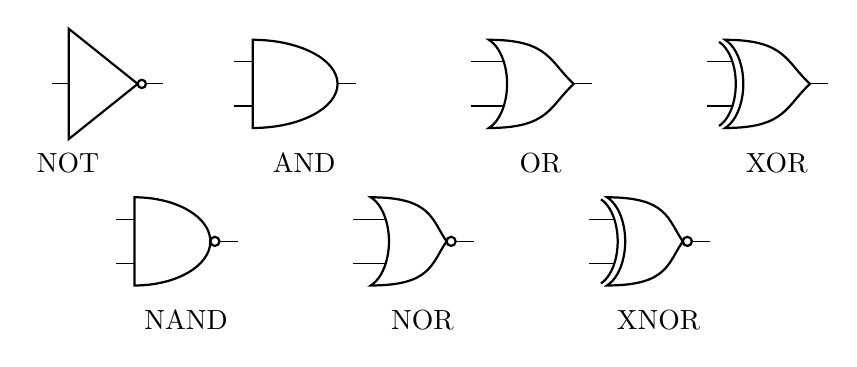
\begin{tikzpicture}
            \node[not port] (NOT) at (0, 0) {};
            \node[and port] (AND) at (3, 0) {};
            \node[or port] (OR) at (6, 0) {};
            \node[xor port] (XOR) at (9, 0) {};
            \node[nand port] (NAND) at (1.5, -2) {};
            \node[nor port] (NOR) at (4.5, -2) {};
            \node[xnor port] (XNOR) at (7.5, -2) {};
            \node at ($(NOT) - (0.5, 1)$) {NOT};
            \node at ($(AND) - (0.5, 1)$) {AND};
            \node at ($(OR) - (0.5, 1)$) {OR};
            \node at ($(XOR) - (0.5, 1)$) {XOR};
            \node at ($(NAND) - (0.5, 1)$) {NAND};
            \node at ($(NOR) - (0.5, 1)$) {NOR};
            \node at ($(XNOR) - (0.5, 1)$) {XNOR};
        \end{tikzpicture}
        \caption{Circuit diagram symbols for NOT, AND, OR, XOR, NAND, NOR, and XNOR.}
        \label{fig:logic gates}
    \end{figure}
    For example the addition operation defined above, called a half adder, can be constructed from an AND gate and an XOR gate as shown in figure~\ref{fig:half adder}.
    \begin{figure}[ht]
        \centering
        \tikzsetnextfilename{classical-half-adder}
        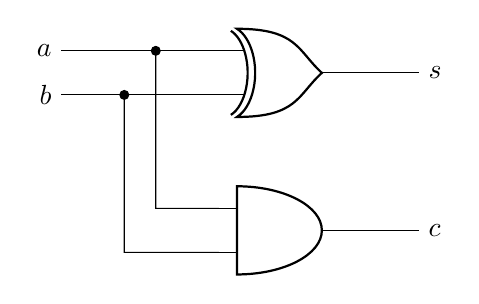
\begin{tikzpicture}
            \node[and port] (AND) at (0, 0) {};
            \node[xor port] (XOR) at (0, 2) {};
            \coordinate (a) at ($(XOR.in 1) - (2, 0)$) {};
            \coordinate (b) at ($(XOR.in 2) - (2, 0)$) {};
            \coordinate (a branch) at ($(a)!.6!(XOR.in 1)$) {};
            \coordinate (b branch) at ($(b)!.4!(XOR.in 2)$) {};
            \coordinate (a right) at (a branch|-AND.in 1) {};
            \coordinate (b right) at (b branch|-AND.in 2) {};
            \coordinate (s) at ($(XOR.out) + (1, 0)$) {};
            \coordinate (c) at ($(AND.out) + (1, 0)$) {};
            \node[left] at (a) {\(a\)};
            \node[left] at (b) {\(b\)};
            \draw (a) to[short] (XOR.in 1);
            \draw (b) to[short] (XOR.in 2);
            \draw (a branch) to[short, *-] (a right) to[short] (AND.in 1);
            \draw (b branch) to[short, *-] (b right) to[short] (AND.in 2);
            \draw (XOR.out) to[short] (s) node[right] {\(s\)};
            \draw (AND.out) to[short] (c) node[right] {\(c\)};
        \end{tikzpicture}
        \caption{Half adder}
        \label{fig:half adder}
    \end{figure}
    Comparing the truth tables XOR and AND we see that the outputs correspond to \(s\) and \(c\) respectively from the half adder.
    
    \subsection{Quantum Computing}
    The field of quantum computing essentially follows the ideas of classical computing but instead of electric currents representing bits we work with state vectors.
    Instead of gates and switches we evolve the state vector to the desired output.
    
    Quantum computing first arose from a practical issue.
    Suppose we have a binary gate with two inputs and one output.
    Because this gate is not reversible some information is necessarily lost when it is used.
    The most efficient possible case would be to have one electron go into each input and then have one electron come out and the other dissipate away.
    The loss of information here leads to an entropy increase of \(\ln 2\).
    If the system is at temperature \(T\) then this leads to generation of heat \(\boltzmann T\ln 2\).
    In a real computer far more than one electron is used and this simply increases the heat released.
    While better designs can reduce the heat output of a computer there is still an intrinsic heat release due to information loss that simply cannot be removed.
    Another concern with classical computing is the breakdown of Moore's law.
    Moore's law, in its simplest form, states that the density of transistors on a chip doubles approximately every two years.
    The problem is that there is a quantum limit to this.
    At some point transistors will becomes so small that quantum effects such as tunnelling cause real problems and transistors simply can't be made smaller.
    Since almost all systems, including logic gates, are implemented with transistors this causes some real problems for the future of computing.
    
    One solution to these problems was the suggestion that computers should be designed so that every operation is reversible.
    It was then suggested that quantum mechanics could be exploited to do this and so quantum computing was birthed.
    Another motivation was that quantum computers could be used to simulate quantum mechanical systems realistically in a way that simply isn't possible with classical computers.
    Many algorithms have been designed to work with quantum computers exploiting quantum mechanics to perform certain tasks orders of magnitude faster than is possible with classical computers.
    
    The basic quantum computer works with a set of \(n\)-qubits.
    A full description then uses states in a Hilbert space of dimension \(2^n\).
    The \(n\)-qubits are formed into tensor product states and these sates are acted on by unitary operators leading to various superpositions of the \(2^n\) basis states.
    The idea is then to use these superpositions to cancel out certain states and leave behind only the desired output.
    The goal is to find a combination of basic operations that leads to something computationally useful.
    This is then called a quantum algorithm.
    
    \subsection{Quantum Registers and Logic Gates}
    In a classical computer the bits of data are held in a register and then the data is accessed and combined using logic gates.
    The language used in quantum computing is similar to this however the implementation is not.
    A quantum register is a state vector.
    For example a one qubit register is simply the state of the qubit, \(\ket{\psi} = a_0\ket{0} + a_1\ket{1}\).
    A two qubit register is state of the two qubit system,
    \[\ket{\psi} = a_{00}\ket{00} + a_{01}\ket{01} + a_{10}\ket{10} + a_{11}\ket{11}.\]
    Higher qubit registers are defined similarly.
    Note that a quantum register of multiple qubits is more complicated than simply multiple copies of a single qubit register as it allows for entanglement.
    
    A standard way to think about quantum computing algorithms is to write the quantum register in the form
    \[\sum_{c, t}a_{ct}\ket{c}_n\tensorProd\ket{t}_m.\]
    Here the first terms, \(c\), are called the control or input register and the second terms, \(t\), are called the target or output register.
    These names don't necessarily match with the actual implementation of the algorithm but we aren't concerned about that here.
    The subscripts \(m\) and \(n\) are simply the number of qubits which is also the length of the binary number needed to specify a state.
    For example \(\ket{c}_4\) is an input register that can take one of \(2^4 = 16\) states labelled from 0 to 15.
    
    A quantum logic gate is an operator that acts on the quantum register.
    Since we are interested in reversible computations most of the operators we consider are unitary and therefore preserve the norm of the quantum register.
    Since the time evolution operator is unitary we can think of these gates as simply controlling the Hamiltonian so that the state evolves in a desirable way.
    Non-unitary operators are also sometimes considered.
    For example making a measurement is generally non-unitary.
    It is also possible that interactions with the environment will cause decoherence in a real life application.
    It is possible that non-unitary operators could be used to reverse these effects.
    Since we are only going to look at introductory quantum computing we will consider all operators to be unitary.
    
    One operator that we have already seen is the Hadamard operator, \(\operator{H}_d\).
    This acts on a single qubit.
    In the two dimensional spinor representation this gate is given by
    \[\operator{H}_d\representation \frac{\sqrt{2}}{2}\twoMat{1}{1}{1}{-1}.\]
    This can be written more abstractly as
    \[\operator{H}_d = \frac{\sqrt{2}}{2}(\ketbra{0}{0} + \ketbra{0}{1} + \ketbra{1}{0} - \ketbra{1}{1}).\]
    Gates can also be represented diagrammaticality as a labelled box:
    \begin{center}
        \tikzsetnextfilename{quantum-gate-1}
        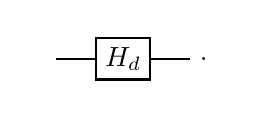
\begin{tikzpicture}
            \tikzstyle{operator} = [draw, fill=white, minimum size=1.5em, thick]
            \matrix[row sep=0.4cm] {
            \node (in) {}; &[0.5cm]
            \node[operator] {\(\operator{H}_d\)}; &[0.5cm]
            \node (out) {.}; \\
            };
            \begin{pgfonlayer}{background}
                \draw[thick] (in) -- (out);
            \end{pgfonlayer}
        \end{tikzpicture}
    \end{center}
    The action of this operator on, for example, the state \(\ket{0}\), is then given by
    \begin{center}
        \tikzsetnextfilename{quantum-gate-2}
        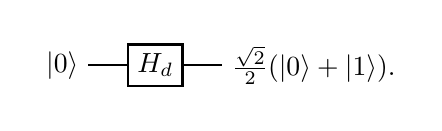
\begin{tikzpicture}
            \tikzstyle{operator} = [draw, fill=white, minimum size=1.5em, thick]
            \matrix[row sep=0.4cm] {
                \node (in) {\(\ket{0}\)}; &[0.5cm]
                \node[operator] {\(\operator{H}_d\)}; &[0.5cm]
                \node (out) {\(\frac{\sqrt{2}}{2}(\ket{0} + \ket{1})\).}; \\
            };
            \begin{pgfonlayer}{background}
                \draw[thick] (in) -- (out);
            \end{pgfonlayer}
        \end{tikzpicture}
    \end{center}
    Other gates that we have met are the Pauli gates which in the two dimensional spinor representation are represented by the Pauli spin matrices,
    \[\sigma_x = \twoMat{0}{1}{1}{0}, \qquad \sigma_y = \twoMat{0}{-i}{i}{0}, \qquad\text{and}\qquad \sigma_z = \twoMat{1}{0}{0}{-1}.\]
    These are written more abstractly as
    \[\operator{\sigma}_x = \operator{X} = \ketbra{1}{0} + \ketbra{0}{1}, \qquad \operator{\sigma}_y = \operator{Y} = i\ketbra{1}{0} - i\ketbra{0}{1}, \qquad\text{and}\qquad \operator{\sigma}_z = \operator{Z} = \ketbra{0}{0} - \ketbra{1}{1}.\]
    Or diagrammatically:
    \begin{center}
        \tikzsetnextfilename{quantum-gate-3}
        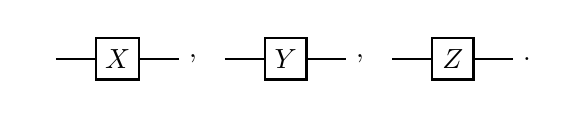
\begin{tikzpicture}
            \tikzstyle{operator} = [draw, fill=white, minimum size=1.5em, thick]
            \matrix[row sep=0.4cm] {
                \node (x in) {}; &[0.5cm]
                \node[operator] {\(\operator{X}\)}; &[0.5cm]
                \node (x out) {,}; &&
                \node (y in) {}; &[0.5cm]
                \node[operator] {\(\operator{Y}\)}; &[0.5cm]
                \node (y out) {,}; & and &
                \node (z in) {}; &[0.5cm]
                \node[operator] {\(\operator{Z}\)}; &[0.5cm]
                \node (z out) {.}; \\
            };
            \begin{pgfonlayer}{background}
                \draw[thick] (x in) -- (x out);
                \draw[thick] (y in) -- (y out);
                \draw[thick] (z in) -- (z out);
            \end{pgfonlayer}
        \end{tikzpicture}
    \end{center}
    These can be generalised further.
    Fore example a generalisation of the Pauli-\(Z\) gate is the \(R_\varphi\) gate which in the two dimensional spinor representation is
    \[\operator{R}_\varphi \representation \twoMat{1}{0}{0}{e^{i\varphi}},\]
    or more abstractly
    \[\operator{R}_\varphi = \ketbra{0}{0} + e^{i\varphi}\ketbra{1}{1},\]
    or diagrammatically
    \begin{center}
        \tikzsetnextfilename{quantum-gate-4}
        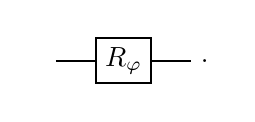
\begin{tikzpicture}
            \tikzstyle{operator} = [draw, fill=white, minimum size=1.5em, thick]
            \matrix[row sep=0.4cm] {
                \node (in) {}; &[0.5cm]
                \node[operator] {\(\operator{R}_\varphi\)}; &[0.5cm]
                \node (out) {.}; \\
            };
            \begin{pgfonlayer}{background}
                \draw[thick] (in) -- (out);
            \end{pgfonlayer}
        \end{tikzpicture}
    \end{center}
    There are also gates that act on two or more qubits at once.
    For example the CNOT gate represented by
    \[\operator{C}\representation\CNOT,\]
    or more abstractly
    \[\operator{C} = \ketbraResize{00}{00} + \ketbra{01}{01} + \ketbra{10}{11} + \ketbra{11}{10},\]
    or diagrammatically
    \begin{center}
        \tikzsetnextfilename{quantum-gate-5}
        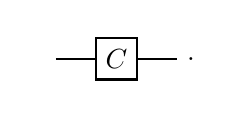
\begin{tikzpicture}
            \tikzstyle{operator} = [draw, fill=white, minimum size=1.5em, thick]
            \matrix[row sep=0.4cm] {
                \node (in) {}; &[0.5cm]
                \node[operator] {\(\operator{C}\)}; &[0.5cm]
                \node (out) {.}; \\
            };
            \begin{pgfonlayer}{background}
                \draw[thick] (in) -- (out);
            \end{pgfonlayer}
        \end{tikzpicture}
    \end{center}
    This gate can also be written in a more detailed form as
    \begin{center}
        \tikzsetnextfilename{quantum-gate-6}
        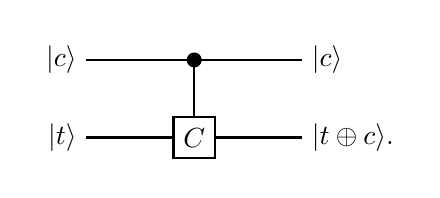
\begin{tikzpicture}
            \tikzstyle{operator} = [draw, fill=white, minimum size=1.5em, thick]
            \tikzstyle{phase} = [draw, fill, shape=circle, minimum size=5pt, inner sep=0pt]
            \matrix[row sep=0.4cm, column sep=0.6cm] {
                % First row
                \node[left] (in1) {\(\ket{c}\)}; &[0.5cm]
                \node[phase] (p) {}; &[0.5cm]
                \node[right] (out1) {\(\ket{c}\)}; \\
                % Second row
                \node[left] (in2) {\(\ket{t}\)}; &[0.5cm]
                \node[operator] (C) {\(\operator{C}\)}; &[0.5cm]
                \node[right] (out2) {\(\ket{t\oplus c}\).}; \\
            };
            \begin{pgfonlayer}{background}
                \draw[thick] (in1) -- (out1);
                \draw[thick] (in2) -- (out2);
                \draw[thick] (p) -- (C);
            \end{pgfonlayer}
        \end{tikzpicture}
    \end{center}
    Here \(\oplus\) is simply addition modulo two which is the same as XOR.
    We can think of CNOT as the reversible version of XOR as the output is \(c\) and \(t \oplus c\) which gives us enough information to determine \(c\) and \(t\).
    This is also sometimes written as
    \begin{center}
        \tikzsetnextfilename{quantum-gate-7}
        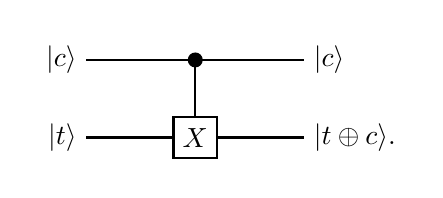
\begin{tikzpicture}
            \tikzstyle{operator} = [draw, fill=white, minimum size=1.5em, thick]
            \tikzstyle{phase} = [draw, fill, shape=circle, minimum size=5pt, inner sep=0pt]
            \matrix[row sep=0.4cm, column sep=0.6cm] {
                % First row
                \node[left] (in1) {\(\ket{c}\)}; &[0.5cm]
                \node[phase] (p) {}; &[0.5cm]
                \node[right] (out1) {\(\ket{c}\)}; \\
                % Second row
                \node[left] (in2) {\(\ket{t}\)}; &[0.5cm]
                \node[operator] (X) {\(\operator{X}\)}; &[0.5cm]
                \node[right] (out2) {\(\ket{t\oplus c}\).}; \\
            };
            \begin{pgfonlayer}{background}
                \draw[thick] (in1) -- (out1);
                \draw[thick] (in2) -- (out2);
                \draw[thick] (p) -- (X);
            \end{pgfonlayer}
        \end{tikzpicture}
    \end{center}
    as we can view \(\operator{C}\) as a block matrix:
    \[\operator{C}\representation \twoMat{\ident}{0}{0}{\operator{X}}.\]
    Note that the order of operators in a diagram is left to right in the order we would think of a circuit passing through gates whereas the order of operators in a product is right to left as with matrix multiplication.
    Hence
    \begin{center}
        \tikzsetnextfilename{quantum-gate-8}
        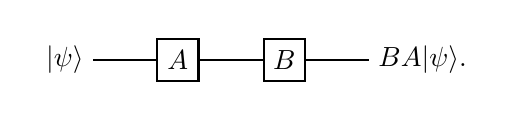
\begin{tikzpicture}
            \tikzstyle{operator} = [draw, fill=white, minimum size=1.5em, thick]
            \matrix[row sep=0.4cm, column sep=0.8cm] {
                \node (in) {\(\ket{\psi}\)}; &%[0.5cm]
                \node[operator] {\(\operator{A}\)}; &%[0.5cm]
                \node[operator] {\(\operator{B}\)}; &%[0.5cm]
                \node[right] (out) {\(\operator{B}\operator{A}\ket{\psi}\).}; \\
            };
            \begin{pgfonlayer}{background}
                \draw[thick] (in) -- (out);
            \end{pgfonlayer}
        \end{tikzpicture}
    \end{center}
    
    \section{Deutsch Algorithm}
    The Deutsch algorithm is one of the simplest quantum computing algorithms and provides useful insight into the key features of many quantum computing algorithms.
    The Deutsch algorithm aims to answer the following question: Given a function, \(f\colon\{1, 0\} \to \{1, 0\}\), that is a function from a bit to a bit, is \(f(0) = f(1)\), that is, is \(f\) constant?
    To answer this question classically we would need to compute \(f(0)\) and \(f(1)\) and compare the results.
    This corresponds to two measurements.
    The Deutsch algorithm gives us a way to make one measurement and it will tell us if \(f\) is constant or not.
    It should be noted that the actual value is not known after this algorithm, just if it is the same for both inputs or different.
    
    A variable that we wish to investigate in quantum computing is often encoded in an operator, \(\operator{O}\), usually called the \define{oracle}.
    The exact specifics of how this is done depend on the object we want to study.
    In this case we wish to know about \(f\) and we define the oracle as an operator on the register with the action
    \[\operator{O}_f (\ket{c}\tensorProd\ket{t}) = \ket{c}\tensorProd\ket{c \oplus f(t)},\]
    where \(\oplus\) is addition modulo 2.
    This can be represented diagrammatically as
    \begin{center}
        \tikzsetnextfilename{deutsch-algorithm-quantum-gate-1}
        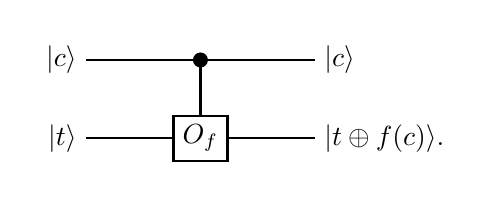
\begin{tikzpicture}
            \tikzstyle{operator} = [draw, fill=white, minimum size=1.5em, thick]
            \tikzstyle{phase} = [draw, fill, shape=circle, minimum size=5pt, inner sep=0pt]
            \matrix[row sep=0.4cm, column sep=0.6cm] {
                % First row
                \node[left] (in1) {\(\ket{c}\)}; &[0.5cm]
                \node[phase] (p) {}; &[0.5cm]
                \node[right] (out1) {\(\ket{c}\)}; \\
                % Second row
                \node[left] (in2) {\(\ket{t}\)}; &[0.5cm]
                \node[operator] (O) {\(\operator{O}_f\)}; &[0.5cm]
                \node[right] (out2) {\(\ket{t\oplus f(c)}\).}; \\
            };
            \begin{pgfonlayer}{background}
                \draw[thick] (in1) -- (out1);
                \draw[thick] (in2) -- (out2);
                \draw[thick] (p) -- (O);
            \end{pgfonlayer}
        \end{tikzpicture}
    \end{center}
    Since the domain and codomain of \(f\) are small we can exactly specify all four possible functions:
    \[
        \begin{array}{c|cc}\hline
            f_i & f_i(0) & f_i(1)\\\hline
            f_1 & 0 & 0\\
            f_2 & 0 & 1\\
            f_3 & 1 & 0\\
            f_4 & 1 & 1\\\hline
        \end{array}
    \]
    We can encode each of these into an oracle, \(\operator{O}_{f_i}\).
    For example the action of \(\operator{O}_{f_2}\) is
    \begin{align*}
        \operator{O}_{f_2}\ket{0}\tensorProd\ket{0} &= \ket{0}\tensorProd\ket{0 \oplus f_2(0)} = \ket{0}\tensorProd\ket{0 \oplus 0} = \ket{0}\tensorProd\ket{0},\\
        \operator{O}_{f_2}\ket{0}\tensorProd\ket{1} &= \ket{0}\tensorProd\ket{1 \oplus f_2(0)} = \ket{0}\tensorProd\ket{1 \oplus 0} = \ket{0}\tensorProd\ket{1},\\
        \operator{O}_{f_2}\ket{1}\tensorProd\ket{0} &= \ket{1}\tensorProd\ket{0 \oplus f_2(1)} = \ket{1}\tensorProd\ket{0 \oplus 1} = \ket{1}\tensorProd\ket{1},\\
        \operator{O}_{f_2}\ket{1}\tensorProd\ket{1} &= \ket{1}\tensorProd\ket{1 \oplus f_2(1)} = \ket{1}\tensorProd\ket{1 \oplus 1} = \ket{1}\tensorProd\ket{0}.
    \end{align*}
    Notice that this is the same action as \(\operator{C}\).
    
    The next step is the actual algorithm which is just a list of operators to apply and a final measurement.
    The process for finding the appropriate operators is mostly trial and error and not very illuminating so we will just give the final algorithm.
    Start with the register \(\ket{0}\tensorProd\ket{0}\), it is common for quantum algorithms to start with a state of the form \(\ket{0}\tensorProd\dotsb\tensorProd\ket{0}\).
    Compute
    \[(\operator{H}_d\tensorProd\ident)\operator{O}_{f} (\operator{H}_d\tensorProd\operator{H}_d) (\operator{X}\tensorProd\operator{X}) (\ket{0}\tensorProd\ket{0}).\]
    Measure the state.
    If you get \(\ket{c} = \ket{0}\) then the function is constant.
    If \(\ket{c} = \ket{1}\) then the function is not constant.
    We will now carry out this algorithm.
    
    First we need to compute
    \[(\operator{X}\tensorProd\operator{X})(\ket{0}\tensorProd\ket{0}).\]
    We do this in the two dimensional tensor product representation:
    \begin{align*}
        \operator{X}\ket{0} &\representation \twoMat{0}{1}{1}{0}\twoVec{1}{0}\\
        &= \twoVec{0}{1}\\
        &\represents \ket{1}
    \end{align*}
    So,
    \[(\operator{X}\tensorProd\operator{X})(\ket{0}\tensorProd\ket{0}) = (\operator{X}\ket{0})\tensorProd(\operator{X}\ket{0}) = \ket{1}\tensorProd\ket{1}.\]
    Next we compute
    \[(\operator{H}_d\tensorProd\operator{H}_d)(\ket{1}\tensorProd\ket{1}),\]
    again in the two dimensional tensor product representation we have
    \begin{align*}
        \operator{H}_d\ket{1} &\representation \frac{\sqrt{2}}{2}\twoMat{1}{1}{1}{-1}\twoVec{0}{1}\\
        &= \frac{\sqrt{2}}{2}\twoVec{1}{-1}\\
        &= \frac{\sqrt{2}}{2}\left[\twoVec{1}{0} - \twoVec{0}{1}\right]\\
        &\represents \frac{\sqrt{2}}{2}(\ket{0} - \ket{1}).
    \end{align*}
    So,
    \begin{align*}
        (\operator{H}_d\tensorProd\operator{H}_d) (\ket{1}\tensorProd\ket{1}) &= (\operator{H}_d\ket{1})\tensorProd (\operator{H}_d\tensorProd\ket{1})\\
        &= \frac{1}{2}(\ket{0} - \ket{1})\tensorProd(\ket{0} - \ket{1})\\
        &= \frac{1}{2}(\ket{0}\tensorProd\ket{0} - \ket{0}\tensorProd\ket{1} - \ket{1}\tensorProd\ket{0} + \ket{1}\tensorProd\ket{1}).
    \end{align*}
    Next we act with the oracle:
    \begin{align*}
        \ket{\psi} &= \operator{O}_f \frac{1}{2}(\ket{0}\tensorProd\ket{0} - \ket{0}\tensorProd\ket{1} - \ket{1}\tensorProd\ket{0} + \ket{1}\tensorProd\ket{1})\\
        &= \frac{1}{2}(\ket{0}\tensorProd\ket{0\oplus f(0)} - \ket{0}\tensorProd\ket{1\oplus f(0)} - \ket{1}\tensorProd\ket{0\oplus f(1)} + \ket{1}\tensorProd\ket{1\oplus f(1)})\\
        &= \frac{1}{2}[\ket{0}\tensorProd(\ket{0\oplus f(0)} - \ket{1\oplus f(0)}) + \ket{1}\tensorProd (-\ket{0\oplus f(1)} + \ket{1\oplus f(1)})].
    \end{align*}
    Finally we apply the Hadamard operator to only the control state.
    In the two dimensional tensor product representation we have
    \begin{align*}
        \operator{H}_d\ket{0} &\representation \frac{\sqrt{2}}{2}\twoMat{1}{1}{1}{-1}\twoVec{1}{0} = \twoVec{1}{1} = \twoVec{1}{0} + \twoVec{0}{1} \represents \frac{\sqrt{2}}{2}(\ket{0} + \ket{1})\\
        \operator{H}_d\ket{1} &\representation \frac{\sqrt{2}}{2}\twoMat{1}{1}{1}{-1}\twoVec{0}{1} = \twoVec{1}{-1} = \twoVec{1}{0} - \twoVec{0}{1} \represents \frac{\sqrt{2}}{2}(\ket{0} - \ket{1})\\
    \end{align*}
    and so,
    \begin{align*}
        (\operator{H}_d\tensorProd\ident)\ket{\psi} &= \frac{\sqrt{2}}{4}[(\ket{0} + \ket{1})\tensorProd(\ket{0\oplus f(0)} - \ket{1\oplus f(0)}) + (\ket{0} - \ket{1})\tensorProd (-\ket{0\oplus f(1)} + \ket{1\oplus f(1)})]\\
        &= \frac{\sqrt{2}}{4} \ket{0} \tensorProd (\ket{0\oplus f(0)} - \ket{1 \oplus f(0)} - \ket{0 \oplus f(1)} + \ket{1 \oplus f(1)})\\
        &+ \frac{\sqrt{2}}{4}\ket{1} \tensorProd (\ket{0\oplus f(0)} - \ket{1\oplus f(0)} + \ket{0\oplus f(1)} - \ket{1\oplus f(1)})\\
        &= \frac{\sqrt{2}}{4} \ket{0} \tensorProd (\ket{f(0)} - \ket{1 \oplus f(0)} - \ket{f(1)} + \ket{1 \oplus f(1)})\\
        &+ \frac{\sqrt{2}}{4}\ket{1} \tensorProd (\ket{f(0)} - \ket{1\oplus f(0)} + \ket{f(1)} - \ket{1\oplus f(1)})\\
    \end{align*}
    Now consider the case when \(f\) is constant so \(f(0) = f(1)\).
    We then have
    \begin{align*}
        (\operator{H}_d\tensorProd\ident)\ket{\psi} &= \frac{\sqrt{2}}{4}\ket{0} \tensorProd (\ket{f(0)} - \ket{1\oplus f(0)} - \ket{f(0)} + \ket{1\oplus f(0)})\\
        &+ \frac{\sqrt{2}}{4}\ket{1}\tensorProd (\ket{f(0)} - \ket{1 \oplus f(0)} + \ket{f(0)} - \ket{1 \oplus f(0)})\\
        &= \frac{\sqrt{2}}{2}\ket{1}\tensorProd (\ket{f(0)} - \ket{1 \oplus f(0)}).
    \end{align*}
    So if we measure this state we will find \(\ket{c} = \ket{1}\).
    If instead \(f(0) \ne f(1)\) then \(1 \oplus f(0) = 0\oplus f(1)\) and \(0 \oplus f(0) = 1\oplus f(1)\).
    Also \(f(0) = 1 \oplus f(1)\) and \(f(1) = 1 \oplus f(0)\).
    Thus
    \begin{align*}
        (\operator{H}_d\tensorProd\ident)\ket{\psi} &= \frac{\sqrt{2}}{4} \ket{0} \tensorProd (\ket{f(0)} - \ket{1 \oplus f(0)} - \ket{1\oplus f(0)} + \ket{f(0)})\\
        &+ \frac{\sqrt{2}}{4}\ket{1} \tensorProd (\ket{f(0)} - \ket{1\oplus f(0)} + \ket{1\oplus f(0)} - \ket{f(0)})\\
        &= \frac{\sqrt{2}}{2}\ket{0} \tensorProd (\ket{f(0)} - \ket{1 \oplus f(0)}).
    \end{align*}
    So if upon measuring the register we get \(\ket{c} = \ket{0}\) we know that \(f(0) \ne f(1)\).
    
    \subsection{Constructing The Oracle}
    When defining a quantum algorithm one should show that all operators are unitary and, if possible, that they can be constructed from elementary gates such as \(\operator{C}\), \(\operator{X}\), etc.
    This is useful as it would allow a general quantum computer to use the algorithm without needing special hardware.
    The only new operator in the Deutsch algorithm is the oracle.
    It is fairly simple to show directly that the oracles can be constructed as follows:
    \begin{align*}
        \operator{O}_{f_1} &= \ident,\\
        \operator{O}_{f_2} &= \operator{C},\\
        \operator{O}_{f_3} &= \operator{C} (\ident \tensorProd \operator{X}),\\
        \operator{O}_{f_4}&= (\operator{I}\tensorProd\operator{X}).
    \end{align*}
    We can construct \(4\times 4\) matrices representing these.
    To do so we need to define the tensor product of two \(2\times 2\) matrices.
    Let \(A\) and \(B\) be \(2\times 2\) matrices with components \(a_{ij}\) and \(b_{ij}\).
    Then
    \[
        A\tensorProd B = \twoMat{a_{11}B}{a_{12}B}{a_{21}B}{a_{22}B} =
        \begin{pmatrix}
            a_{11}b_{11} & a_{11}b_{12} & a_{12}b_{11} & a_{12}b_{12}\\
            a_{11}b_{21} & a_{11}b_{21} & a_{12}b_{21} & a_{12}b_{21}\\
            a_{21}b_{11} & a_{21}b_{12} & a_{22}b_{11} & a_{22}b_{12}\\
            a_{21}b_{21} & a_{21}b_{21} & a_{22}b_{21} & a_{22}b_{21}
        \end{pmatrix}
        .
    \]
    This generalises to higher dimensional matrices as well.
    This allows us to write terms like \(\ident\tensorProd\operator{X}\) as \(4\times 4\) matrices.
    Thus the four oracles in this representation and as quantum circuits are given by
    \begin{align*}
        \operator{O}_{f_1} &= \ident\\
        &\representation
        \begin{pmatrix}
            1 & 0 & 0 & 0\\
            0 & 1 & 0 & 0\\
            0 & 0 & 1 & 0\\
            0 & 0 & 0 & 1
        \end{pmatrix}
        \\
        &= \tikzsetnextfilename{deutsch-algorithm-quantum-gate-2}
        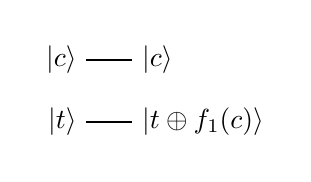
\begin{tikzpicture}[baseline=(current bounding box.center)]
            \tikzstyle{operator} = [draw, fill=white, minimum size=1.5em, thick]
            \tikzstyle{phase} = [draw, fill, shape=circle, minimum size=5pt, inner sep=0pt]
            \matrix[row sep=0.2cm, column sep=0.6cm] {
                % First Row
                \node[left] (in1) {\(\ket{c}\)}; \pgfmatrixnextcell
                \node[right] (out1) {\(\ket{c}\)}; \\
                % Second Row
                \node[left] (in2) {\(\ket{t}\)}; \pgfmatrixnextcell
                \node[right] (out2) {\(\ket{t \oplus f_1(c)}\)}; \\
            };
            \begin{pgfonlayer}{background}
                \draw[thick] (in1) -- (out1);
                \draw[thick] (in2) -- (out2);
            \end{pgfonlayer}
        \end{tikzpicture}
        \\
        \operator{O}_{f_2} &= \operator{C}\\
        &\representation \CNOT\\
        &= \tikzsetnextfilename{deutsch-algorithm-quantum-gate-3}
        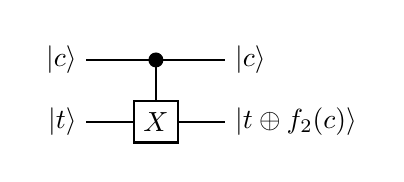
\begin{tikzpicture}[baseline=(current bounding box.center)]
            \tikzstyle{operator} = [draw, fill=white, minimum size=1.5em, thick]
            \tikzstyle{phase} = [draw, fill, shape=circle, minimum size=5pt, inner sep=0pt]
            \matrix[row sep=0.2cm, column sep=0.6cm] {
                % First Row
                \node[left] (in1) {\(\ket{c}\)}; \pgfmatrixnextcell
                \node[phase] (P) {}; \pgfmatrixnextcell
                \node[right] (out1) {\(\ket{c}\)}; \\
                % Second Row
                \node[left] (in2) {\(\ket{t}\)}; \pgfmatrixnextcell
                \node[operator] (X) {\(\operator{X}\)}; \pgfmatrixnextcell
                \node[right] (out2) {\(\ket{t \oplus f_2(c)}\)}; \\
            };
            \begin{pgfonlayer}{background}
                \draw[thick] (in1) -- (out1);
                \draw[thick] (in2) -- (out2);
                \draw[thick] (P) -- (X);
            \end{pgfonlayer}
        \end{tikzpicture}
        \\
        \operator{O}_{f_3} &= \operator{C}(\ident \tensorProd \operator{X})\\
        &\representation
        \begin{pmatrix}
            0 & 1 & 0 & 0\\
            1 & 0 & 0 & 0\\
            0 & 0 & 1 & 0\\
            0 & 0 & 0 & 1
        \end{pmatrix}
        \\
        &= \tikzsetnextfilename{deutsch-algorithm-quantum-gate-4}
        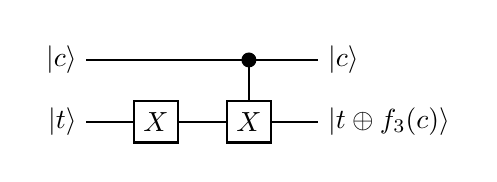
\begin{tikzpicture}[baseline=(current bounding box.center)]
            \tikzstyle{operator} = [draw, fill=white, minimum size=1.5em, thick]
            \tikzstyle{phase} = [draw, fill, shape=circle, minimum size=5pt, inner sep=0pt]
            \matrix[row sep=0.2cm, column sep=0.6cm] {
                % First Row
                \node[left] (in1) {\(\ket{c}\)}; \pgfmatrixnextcell
                \node[left] {}; \pgfmatrixnextcell
                \node[phase] (P) {}; \pgfmatrixnextcell
                \node[right] (out1) {\(\ket{c}\)}; \\
                % Second Row
                \node[left] (in2) {\(\ket{t}\)}; \pgfmatrixnextcell
                \node[operator] {\(\operator{X}\)}; \pgfmatrixnextcell
                \node[operator] (X) {\(\operator{X}\)}; \pgfmatrixnextcell
                \node[right] (out2) {\(\ket{t \oplus f_3(c)}\)}; \\
            };
            \begin{pgfonlayer}{background}
                \draw[thick] (in1) -- (out1);
                \draw[thick] (in2) -- (out2);
                \draw[thick] (P) -- (X);
            \end{pgfonlayer}
        \end{tikzpicture}
        \\
        \operator{O}_{f_4} &= \ident\tensorProd\operator{X}\\
        &\representation
        \begin{pmatrix}
            0 & 1 & 0 & 0\\
            1 & 0 & 0 & 0\\
            0 & 0 & 0 & 1\\
            0 & 0 & 1 & 0
        \end{pmatrix}
        \\
        &= \tikzsetnextfilename{deutsch-algorithm-quantum-gate-5}
        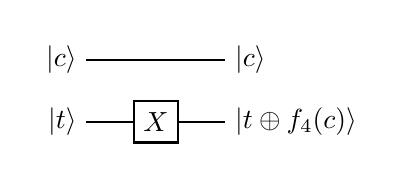
\begin{tikzpicture}[baseline=(current bounding box.center)]
            \tikzstyle{operator} = [draw, fill=white, minimum size=1.5em, thick]
            \tikzstyle{phase} = [draw, fill, shape=circle, minimum size=5pt, inner sep=0pt]
            \matrix[row sep=0.2cm, column sep=0.6cm] {
                % First Row
                \node[left] (in1) {\(\ket{c}\)}; \pgfmatrixnextcell
                \node {}; \pgfmatrixnextcell
                \node[right] (out1) {\(\ket{c}\)}; \\
                % Second Row
                \node[left] (in2) {\(\ket{t}\)}; \pgfmatrixnextcell
                \node[operator] {\(\operator{X}\)}; \pgfmatrixnextcell
                \node[right] (out2) {\(\ket{t \oplus f_4(c)}\)}; \\
            };
            \begin{pgfonlayer}{background}
                \draw[thick] (in1) -- (out1);
                \draw[thick] (in2) -- (out2);
            \end{pgfonlayer}
        \end{tikzpicture}
    \end{align*}
    
    \section{Grover's Algorithm}
    Grover's algorithm can be stated in many ways.
    It can be thought of as a search algorithm which finds a given state in a quantum register or as a way to probe an unknown oracle and find the state that it picks out.
    The algorithm starts with the state \(\ket{0}^{\tensorProd N}\) where
    \[\ket{0}^{\tensorProd N} = \underbrace{\ket{0}\tensorProd\ket{0} \tensorProd\dotsb\tensorProd \ket{0}}_{N~\text{times}},\]
    and \(N\) is the number of things we have to search through.
    Then the Hadamard operator is applied to each term which results in the state \(\operator{H}_d^{\tensorProd N} \ket{0}^{\tensorProd N}\) which is a linear combination of all basis states such that all states have equal probability.
    We will consider for an example here the case \(n = 3\).
    The starting state is then \(\ket{000}\) and the first step gives us
    \[\ket{\psi} = (\operator{H}_d\tensorProd \operator{H}_d\tensorProd \operator{H}_d)\ket{000} = \frac{\sqrt{2}}{4}(\ket{000} + \ket{001} + \ket{010} + \ket{100} + \ket{011} + \ket{101} + \ket{110} + \ket{111}).\]
    Suppose we have an oracle that picks out the state \(\ket{s}\).
    The Grover algorithm gives us a way to move the system towards this state in a unitary manner.
    This is important as it means that operations are reversible and we can continue to use the state for further computations after the algorithm.
    Compare this to the normal way we pick out a state by simply taking the inner product with \(\bra{s}\).
    
    The next step of the Grover algorithm is to apply the oracle, \(\operator{O}\), which flips the sign of the state, \(\ket{s}\), which it is singling out.
    This oracle is given by
    \[\operator{O} = \ident - 2\ketbra{s}{s}.\]
    This has a diagonal matrix representation of ones down the diagonal
    except for the entry associated with \(\ket{s}\) which has a \(-1\).
    
    Suppose for our example that \(\ket{s} = \ket{110}\).
    Then the action of the oracle is
    \[\ket{\psi_-} = \operator{O}\ket{\psi} = \frac{\sqrt{2}}{4}(\ket{000} + \ket{001} + \ket{010} + \ket{100} + \ket{011} + \ket{101} - \ket{110} + \ket{111}).\]
    The only change is that the coefficient of \(\ket{s} = \ket{110}\) is now negative.
    
    The next step of the algorithm is to apply the Grover operation,
    \[\operator{G} = 2\ketbra{\psi}{\psi} - \ident\]
    which for our example gives us
    \[\ket{\psi_d} = \frac{\sqrt{2}}{8}(\ket{000} + \ket{001} + \ket{010} + \ket{100} + \ket{011} + \ket{101} + 5\ket{110} + \ket{111}).\]
    Notice that the net effect of \(\operator{G}\operator{O}\) is to increase the probability of measuring the register in the state \(\ket{s}\).
    It turns out that applying \(\operator{G}\operator{O}\) iteratively \(\sqrt{N}\) times will cause \(\ket{s}\) to have its maximum amplitude.
    So if we do this then measure the register it is likely that we will measure the state \(\ket{s}\).
    
    We can better understand this algorithm by considering the action of \(\operator{O}\) and \(\operator{G}\) on the desired state \(\ket{s}\) and the initial state \(\ket{\psi} = \operator{H}_d^{\tensorProd N}\ket{0}^{\tensorProd N}\):
    \begin{align*}
        \operator{O}\ket{s} &= -\ket{s},\\
        \operator{O}\ket{\psi} &= \ket{\psi} - \frac{2}{\sqrt{N}}\ket{s},\\
        \operator{G}\ket{s} &= \frac{2}{\sqrt{N}}\ket{\psi} - \ket{s},\\
        \operator{G}\ket{\psi} &= \ket{\psi}.
    \end{align*}
    We see that the action of both operators always returns a linear combination of \(\ket{s}\) and \(\ket{\psi}\).
    This means that the action of \(\operator{G}\operator{O}\) on \(\ket{\psi}\) will be another state in the two dimensional subspace spanned by \(\ket{\psi}\) and \(\ket{s}\).
    
    We can write an arbitrary state, \(\ket{u}\in\hilbert\), as
    \[\ket{u} = a\ket{s_\perp} + b\ket{s}\]
    where \(\ket{s_\perp}\) is some state perpendicular to \(\ket{s}\) so \(\braket{s}{s_\perp} = 0\).
    Note that this is not a basis for the whole space as another state, \(\ket{v}\in\hilbert\) may require a different \(\ket{s_\perp}\) but all states can be decomposed this way.
    Similarly we can write an arbitrary state, \(\ket{u'}\in\hilbert\) as
    \[\ket{u'} = a\ket{\psi} + b\ket{\psi_\perp}\]
    where \(\ket{\psi_\perp}\) is perpendicular to \(\ket{\psi}\) so \(\braket{\psi}{\psi_\perp} = 0\).
    
    The first step of Grover's algorithm is to act on \(\ket{\psi}\) with \(\operator{O}\).
    We can decompose \(\ket{\psi}\) in terms of \(\ket{s}\) and \(\ket{s_\perp}\).
    First note that since each coefficient in \(\ket{\psi}\) is equal for a properly normalised state we must have \(\braket{s}{\psi} = N^{-1/2}\) and so
    \begin{align*}
        \operator{O}\ket{\psi} &= \operator{O}\left(\sqrt{\frac{N-1}{N}}\ket{s_\perp} + \frac{1}{\sqrt{N}}\ket{s}\right)\\
        &= \sqrt{\frac{N - 1}{N}}\ket{s_\perp} - \frac{1}{\sqrt{N}}\ket{s}.
    \end{align*}
    We can consider this geometrically as a reflection of \(\ket{\psi}\) in the \(\ket{s}\) axis, see figure~\ref{fig:action of O in grover algorithm as a reflection}.
    \begin{figure}[ht]
        \centering
        \tikzsetnextfilename{grover-algorithm-action-of-O}
        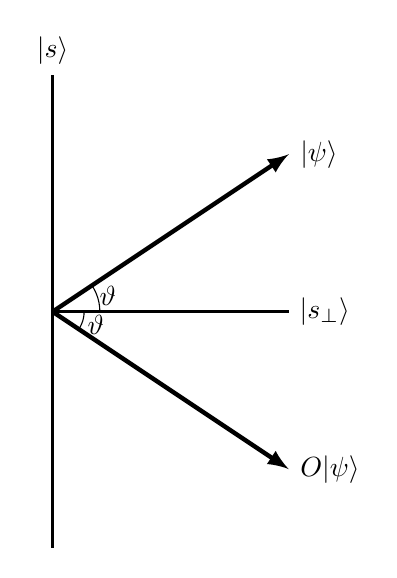
\begin{tikzpicture}
            \tikzset{axis/.style={very thick}}
            \tikzset{vector/.style={ultra thick, ->, >=latex}}
            \draw[axis] (0, -3) -- (0, 3) node[above] {\(\ket{s}\)};
            \draw[axis] (0, 0) -- (3, 0) node[right] {\(\ket{s_\perp}\)};
            \draw[vector] (0, 0) -- (3, 2) node[right] {\(\ket{\psi}\)};
            \draw[vector] (0, 0) -- (3, -2) node[right] {\(\operator{O}\ket{\psi}\)};
            \begin{scope}
                \clip (0, 0) -- (3, 2) -- (3, 0) -- cycle;
                \draw (0, 0) circle [radius=0.6cm];
            \end{scope}
            \begin{scope}
                \clip (0, 0) -- (3, -2) -- (3, 0) -- cycle;
                \draw (0, 0) circle [radius=0.4cm];
            \end{scope}
            \node at (0.7, 0.2) {\(\vartheta\)};
            \node at (0.55, -0.17) {\(\vartheta\)};
        \end{tikzpicture}
        \caption{The action of \(\operator{O}\) on \(\ket{\psi}\) can be viewed as a reflection in the \(\ket{s}\) axis.}
        \label{fig:action of O in grover algorithm as a reflection}
    \end{figure}
    Notice that if \(\ket{\psi}\) makes an angle\footnote{for some definition of angles in a non-Euclidean complex vector space} of \(\vartheta\) to \(\ket{s_{\perp}}\) then the action of \(\operator{O}\) is a rotation through \(-2\vartheta\).
    
    The action of \(\operator{G}\) can be similarly interpreted as a reflection in the line defined by the original state \(\ket{\psi}\).
    This can also be viewed as a rotation through \(4\vartheta\) and so \(\operator{G}\operator{O}\) has a net result of a rotation of \(2\vartheta\) towards \(\ket{s}\).
    
    Each iterative application of \(\operator{G}\operator{O}\) rotates the state \(2\vartheta\) towards \(\ket{s}\).
    At some point we will overshoot \(\ket{s}\) and start moving away again.
    We need to know how many times to apply \(\operator{G}\operator{O}\) to maximise the probability of measuring the register to be in state \(\ket{s}\).
    
    The initial angle, \(\vartheta\), is related to the original state as shown in figure~\ref{fig:relation between s, psi, and theta}.
    \begin{figure}[ht]
        \centering
        \tikzsetnextfilename{grover-algorithm-psi-decomposed-to-s-and-s-perpendicular}
        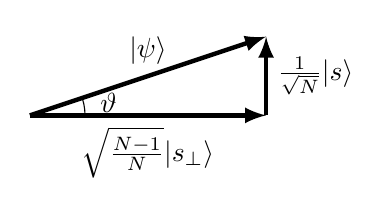
\begin{tikzpicture}
            \tikzset{vector/.style={ultra thick, ->, >=latex}}
            \draw[vector] (0, 0) -- (3, 0) node[midway, below] {\(\sqrt{\frac{N-1}{N}}\ket{s_\perp}\)};
            \draw[vector] (3, 0) -- (3, 1) node[midway, right] {\(\frac{1}{\sqrt{N}}\ket{s}\)};
            \draw[vector] (0, 0) -- (3, 1) node[midway, above] {\(\ket{\psi}\)};
            \begin{scope}
                \clip (0, 0) -- (3, 0) -- (3, 1) -- cycle;
                \draw (0, 0) circle [radius=0.7cm];
            \end{scope}
            \node at (1, 0.16) {\(\vartheta\)};
        \end{tikzpicture}
        \caption{\(\ket{\psi}\) decomposed into \(\ket{s_\perp}\) and \(\ket{s}\) components.}
        \label{fig:relation between s, psi, and theta}
    \end{figure}
    We see that
    \[\sin\vartheta = \frac{1}{\sqrt{N}}.\]
    For large \(N\) \(\vartheta\) must be small so we have \(\vartheta\approx N^{-1/2}\).
    Similarly \(\ket{\psi}\) is almost entirely aligned with \(\ket{s_\perp}\) so we need to rotate it through an angle of \(\pi/2\) to be aligned in the \(\ket{s}\) direction.
    Since each iteration moves us an angle \(2\vartheta \approx 2/\sqrt{N}\) we need \(\pi/(4\vartheta) = \pi\sqrt{N}/4\) (or the closest integer to this) iterations  to reach maximal probability of measuring \(\ket{s}\).
    
    To implement this algorithm one needs to be able to construct \(\operator{O}\) and \(\operator{G}\) from basic gates.
    This can be done but is not very illuminating and quite involved so we won't do it here.
    
    We mentioned at the start of this section that the Grover algorithm can be seen as a search algorithm.
    The context for this is as follows: suppose we have a quantum register, \(\ket{\varphi}\), and we wish to know if a given state, \(\ket{s}\), is in this register.
    Then we use the Grover algorithm as described above and after \(\sqrt{N}\) iterations we measure the register and we expect to measure \(\ket{s}\) with high probability\footnote{with high probability is used here in the technical sense that an event with probability on \(N\) occurs with high probability iff that probability goes to one as \(N\to\infty\).} if \(\ket{s}\) is in \(\ket{\varphi}\).
    From this we conclude that the Grover algorithm, when thought of as a search algorithm searching \(N\) qubits, is \(\order(\sqrt{N})\) since we need to apply \(\operator{G}\operator{O}\) \(\order(\sqrt{N})\) times.
    This is much faster than similar classical search algorithms which are \(\order(N)\).
    
    Quantum computing is still a developing field.
    One of the key features is the ability to explore multiple solutions at once by studying superpositions of states.
    For example a system of \(n\) spin 1/2 particles has \(N = 2^n\) possible states so by studying 10 particles we can study \(2^{10} = 1024\) different states.
    The number of different states grows exponentially with the size of the system.
    If each state corresponds with a possible solution then we can test many solutions at once.
    
    One hope that is held for quantum computing is the ability to solve problems that fall in a class called \NPcomplexity problems.
    \NPcomplexity stands for non-deterministic polynomial time which, roughly speaking, means that once a solution is found we can check that this is a solution in polynomial time.
    That is for a given \NPcomplexity problem there is an algorithm that will return true or false for a given solution and that algorithm is \(\order(N^n)\) for some integer \(n\) and input size \(N\).
    While a solution for a \NPcomplexity problem can be found in polynomial time whether a solution can be found in polynomial time for all \NPcomplexity problems is an open question\footnote{see  \href{https://en.wikipedia.org/wiki/P_versus_NP_problem}{\Pcomplexity vs. \NPcomplexity}}.
    
    For an example of an \NPcomplexity problem consider the task of finding a particular number in a set of all \(n\)-digit numbers which are randomly ordered.
    If we were to simply check every number then the time take grows exponentially with \(n\) (as there are \(\order(10^n)\) \(n\)-digit numbers).
    On the other hand if someone has already found the number in the list then we simply need to check each digit to check it is the correct number and the number of digits grows linearly with \(n\) (as the number of digits \emph{is} \(n\)).
    
    It is possible that a quantum computing algorithm exists which allows us to solve \NPcomplexity problems faster.
    Suppose we have a system of \(n\) spin 1/2 particles.
    If we can somehow find a correspondence between the \(2^n\) states with set of solutions and apply a quantum algorithm to the system which enhances the probability amplitude of the correct answer it is possible that this would lead to an answer faster than any classical algorithm can find a solution.
    Grover's algorithm is the most simple example where this is possible.
    We manipulate the probability amplitudes to find the desired state in \(\order(\sqrt{N})\) as opposed to the classical \(\order(N)\) algorithms.
    
    \section{Information Theory}
    \subsection{Classical Information Theory}
    Information theory is the study of messages and communications with the goal of developing efficient communication.
    The formal meaning of this is as follows.
    A (formal) \define{language} is a set of \(N\) symbols, \(\Sigma = \{s_1, \dotsc, s_N\}\).
    These can be arranged into a \define{message}, \(X\), which is an ordered set of symbols of length \(M_X\), \(X = s_{i}^{1}s_{j}^{2}\dotsm s_{k}^{M_X}\) where superscripts denote position in the message and subscripts take values from 1 to \(N\) such that \(s_i\in\Sigma\).
    At this point there is an important decision to make.
    We need to decide what we care about.
    If we only care about a few possible messages then we can be very efficient by simply assigning each a number and sending that number.
    If we want to be able to send arbitrary messages then  we need to consider the entire language.
    In the following this decision reveals itself whenever there is a sum or we count something we need to choose to sum over or count the part of the language that we care about.
    
    If we denote by \(M_i^X\) then number of times the symbol \(s_i\) appears in the message \(X\) then the frequency, or probability, of \(s_i\) is \(f_i = p_i = M_i^X/M_X\).
    We say that the \define{information} of the symbol \(s_i\) with probability \(p_i\) is
    \[I(p_i) = -\log_2p_i.\]
    Notice that this logarithm is taken in base 2.
    This is because we want to measure information in bits.
    The information of a symbol is a useful quantity when we are studying a large number of symbols.
    Roughly the information characterises how much we learn when we are sent a particular symbol.
    In the extreme case of a language with only one symbol or where we restrict messages to be only one message the information is zero as we know what every message is before it is sent.
    In a language with two symbols with equal probability the information of either symbol is 1 as we learn one thing when the message is sent (we learn which symbol was sent).
    
    The \define{Shannon entropy} of a message is the average information of all symbols:
    \[\shannonEntropy = -\sum_i p_i\log_2 p_i.\]
    This has units of bits per symbol.
    The Shannon source coding theorem states that the Shannon entropy is the minimum number of bits needed to encode the message.
    
    For a first example suppose we have a language of two symbols, \(\{A, B\}\).
    Suppose that the probability of \(A\) is \(p_A\).
    Then the Shannon entropy is
    \[\shannonEntropy = -p_A\log_2p_A - (1 - p_A)\log_2p_A.\]
    This is zero in the limits when \(p_A = 0, 1\) and peaks at \(p_A = 0.5\) with \(\shannonEntropy = \SI{1}{\bitsSI/\symbolSI}\)\footnote{This function may be familiar from the entropy in statistical mechanics}.
    The case of \(p_A = 0.5\) is equivalent to choosing randomly between \(A\) and \(B\) and the Shannon source coding theorem simply states that it requires one bit of information to tell someone which one we chose.
    
    For a more realistic (but only slightly) example we need more symbols.
    Consider a language of four symbols, \(\{A, B, C, D\}\), with  probabilities \(0.5\), \(0.25\), \(0.125\), and \(0.125\) respectively.
    The Shannon entropy of this language is
    \[\shannonEntropy = -0.5\log_20.5 - 0.25\log_20.25 - 0.125\log_20.125 - 0.125\log_20.125 = \SI{1.75}{\bitsSI/\symbolSI}.\]
    So we need at least \(\SI{1.75}{\bitsSI/\symbolSI}\) to encode a character in this language.
    For example consider the following encoding:
    \begin{center}
        \begin{tabular}{cc}\hline
            Symbol & Encoding\\\hline
            \(A\) & 1\\
            \(B\) & 01\\
            \(C\) & 001\\
            \(D\) & 000\\\hline
        \end{tabular}
    \end{center}
    This encoding seems a bit odd at first, why not just use \(0\) for \(A\), 1 for \(B\), \(10\) for \(C\) and \(11\) for \(D\)?
    Because then there is ambiguity, for example \(10\) could be either \(AB\) or \(C\).
    Computers don't have this issue as they work with fixed blocks of bits or use an extra symbol to denote the end of a symbol but this is not the most efficient way to encode.
    Notice that the information of each of the symbols above is equal to the number of bits in the encoding.
    Suppose we want to encode the message \(AABABACD\).
    Then our encoded message is \(11011011001000\).
    This is \(\SI{14}{\bitsSI}\) and as the message is 8 symbols long the information per symbol is \(\SI{14}{\bitsSI}/\SI{8}{\symbolSI} = \SI{1.75}{\bitsSI/\symbolSI}\).
    So we have achieved maximum efficiency in our encoding.
    Note that this limit is for the \emph{average} message.
    If we want to send \(AAAA\) the this can be done in four bits so the Shannon entropy is \(\SI{1}{\bitsSI/\symbolSI}\).
    Similarly if we want to send \(CDCD\) then this requires \(\SI{12}{\bitsSI}\) so the Shannon entropy is \(\SI{3}{\bitsSI/\symbolSI}\).
    
    The idea when encoding a language is that we want the highest frequency bit to have the shortest possible encoding, hence why we chose \(A\) to have a single bit encoding in the example above.
    There is one way that we can improve on this information rate.
    We can encode words.
    Suppose that the string we encoded before, \(AABABACD\), is representative of all messages in the language.
    Notice that \(AA\) appears once, \(BA\) appears twice, and \(CD\) appears once.
    The Shannon entropy of \(\{AA, BA, CD\}\) is \(\SI{1.5}{\bitsSI/\symbolSI}\).
    If we encode \(AB\) as \(1\), \(AA\) as \(01\) and \(CD\) as \(001\) then we can encode our message as \(0111001\) which is \(\SI{7}{bits}\) for 14 symbols\footnote{the hit, quantum physics, sequel to seven brides for seven brothers featuring hit songs such as barn raise(ing and lowering operators) and bless your beautiful hide(rogen atom)}, so one bit better than before.
    However there are now messages we can't encode, for example \(BACCDB\).
    
    \subsection{Quantum Information Theory}
    \subsubsection{Density Matrix}\label{sec:density matrix}
    The stats that we have dealt with so far are what are called \define{pure states}.
    This means that they are a linear combination of basis states.
    The other type of state is a \define{mixed state}.
    These are collections of pure states with some classical probability associated with them.
    These most commonly arise when we aren't certain what pure state a system is in but we do know what the probability of a given state is.
    The probabilities here are classical in that they aren't inherent to the system but are due to our lack of knowledge of the system.
    
    To account for both possibilities we define the \define{density matrix}:
    \[\operator{\rho} = \sum_i p_i\ketbra{\chi_i}{\chi_i}\]
    where \(p_i\) is the classical probability of the state \(\ket{\chi_i}\) from the mixed state.
    The density matrix for a pure state, \(\ket{\chi}\), is simply the projection operator, \(\ketbra{\chi}{\chi}\).
    Some useful properties of the density matrix are:
    \begin{itemize}
        \item \emph{Hermitian} -- This follows since \(\hermit\) distributes over addition and \((\ketbra{\chi}{\chi})\hermit = \ketbra{\chi}{\chi}\).
        
        \item \emph{Trace property} -- The trace of the density matrix is \(\Tr(\operator{\rho}) = 1\).
        To see this let \(\{\ket{\varphi_i}\}\) be a complete set of states.
        Then
        \begin{align*}
            \Tr(\operator{\rho}) &= \sum_{j} \rho_{jj}\\
            &= \sum_{j} \bra{\varphi_j}\operator{\rho}\ket{\varphi_j}\\
            &= \sum_{ij} \bra{\varphi_j} p_i\ket{\chi_i} \braket{\chi_i}{\varphi_j}\\
            &= \sum_i p_i \sum_j \braket{\varphi_j}{\chi_i} \braket{\chi_i}{\varphi_j}\\
            &= \sum_i p_i \sum_j \braket{\chi_i}{\varphi_j} \braket{\varphi_j}{\chi_i}\\
            &= \sum_i p_i \braket{\chi_i}{\chi_i}\\
            &= \sum_i p_i\\
            &= 1.
        \end{align*}
        
        \item \emph{Positive-semidefinite} -- For all \(\ket{\varphi}\in\hilbert\)
        \[\bra{\varphi}\operator{\rho}\ket{\varphi} = \sum_i p_i \braket{\varphi}{\chi_i}\braket{\chi_i}{\varphi} = \sum_i p_i \abs{\braket{\varphi}{\chi_i}}^2 \ge 0.\]
        
        \item \emph{Eigenvalues lie in \([0, 1]\)} -- Let \(\alpha_i\) be the eigenvalues of \(\operator{\rho}\).
        Since \(\operator{\rho}\) is Hermitian it only has real eigenvalues.
        Since \(\operator{\rho}\) is positive-semidefinite it's eigenvalues are non-negative.
        In the eigenbasis of \(\operator{\rho}\) it is diagonal with it's eigenvalues on the diagonal.
        The trace is invariant under change of basis so the trace is 1 meaning \(\sum_i \alpha_i = 1\).
        The only way for positive real numbers to sum to one is if all of those numbers are less than 1.
        
        \item \emph{Trace property for \(\operator{\rho}^2\)} -- \(\Tr(\operator{\rho}^2) \le 1\).
        In the eigenbasis of \(\operator{\rho}\) we have \(\Tr(\operator{\rho}^2) = \sum_i\alpha_i^2\).
        By the triangle inequality
        \[1 = \left[\sum_i \alpha_i\right] \ge \sum_i \alpha_i\]
    \end{itemize}
    Consider now the special case of a pure state.
    Then \(\operator{\rho}^2 = \sum_i\alpha_i^2\ketbra{\alpha_i}{\alpha_i}\) so \(\operator{\rho}^2 = \operator{\rho}\).
    Hence if \(\Tr(\operator{\rho}^2) = 1\) or \(\operator{\rho}^2 = \operator{\rho}\) then \(\operator{\rho}\) represents a pure state.
    
    \subsubsection{Von Neumann Entropy}
    The \define{von Neummann entropy} is defined as
    \[\vonNeumannEntropy = -\Tr(\operator{\rho}\log_2\operator{\rho}),\]
    where \(\log_2\) is applied element wise.
    It is, in many ways, the quantum analogue of the Shannon entropy.
    Consider, for example, the case of a mixed state where each state, \(\ket{\varphi_i}\), appears with probability \(p_i\), and \(\{\ket{\varphi_i}\}\) are mutually orthogonal.
    In this case we can express the density matrix as a diagonal matrix in the \(\{\ket{\varphi_i}\}\) basis.
    In this case
    \begin{align*}
        \vonNeumannEntropy &= -\Tr[\operator{\rho}\log_2\operator{\rho}]\\
        &= -\Tr \left[ 
            \begin{pmatrix}
                p_1    & 0      & \dots  & 0   \\
                0      & p_2    & \dots  & 0   \\
                \vdots & \vdots & \ddots & 0   \\
                0      & 0      & \dots  & p_N
            \end{pmatrix}
            \begin{pmatrix}
                \log_2p_1 & 0         & \dots  & 0         \\
                0         & \log_2p_2 & \dots  & 0         \\
                \vdots    & \vdots    & \ddots & 0         \\
                0         & 0         & \dots  & \log_2p_N
            \end{pmatrix}
        \right]\\
        &= - \Tr
        \begin{pmatrix}
            p_1\log_2p_1    & 0               & \dots  & 0            \\
            0               & p_2\log_2p_2    & \dots  & 0            \\
            \vdots          & \vdots          & \ddots & 0            \\
            0               & 0               & \dots  & p_N\log_2p_N
        \end{pmatrix}
        \\
        &= \sum_i p_i\log_2 p_i\\
        &= \shannonEntropy.
    \end{align*}
    So for orthogonal mixed states the von Neumann entropy reduces to the Shannon entropy.
    Consider instead the case of a pure state, \(\ket{\varphi}\).
    The density matrix is the \(\operator{\rho} = \ketbra{\varphi}{\varphi}\).
    In this case \(\operator{\rho}\) can be expressed as a matrix that is zero everywhere apart from the diagonal element corresponding to \(\ket{\varphi}\) in some basis including \(\ket{\varphi}\) as a basis vector.
    In this slot it will be 1.
    Since \(\log_2 1 = 0\) the von Neumann entropy will be zero.
    This is analogous to the case of a language of a single symbol.
    
    The von Neumann entropy starts to differ from the Shannon entropy when we consider a mixture of non-orthogonal quantum states.
    For example consider the set of two spin states, one spin up along the \(z\)-axis, \(\ket{+}\), and one spin up along the \(y\) axis, \(\ket{y} = \sqrt{2}(\ket{-} + i\ket{+})/2\).
    Suppose both states occur with equal probability in the mixed state.
    The density matrix in the \(\{\ket{+}, \ket{-}\}\) basis is then
    \begin{align*}
        \operator{\rho} &= 0.5\ketbra{+}{+} + 0.5\left[\frac{\sqrt{2}}{2}(i\ket{+} + \ket{-})\right] \left[\frac{\sqrt{2}}{2}(-i\ket{+} + \ket{-})\right]\\
        &= \left( 0.5 + i\frac{1}{2} \right)\ketbra{+}{+} + 0.5i\frac{1}{2}\ketbra{+}{-} - 0.5i\frac{1}{2}\ketbra{-}{+} + 0.5\frac{1}{2}\ketbra{-}{-}\\
        &= 
        \begin{pmatrix}
            0.75   & 0.25i\\
            -0.25i & 0.25
        \end{pmatrix}
        .
    \end{align*}
    The eigenvalues of this matrix are \(\alpha_1 = 0.146\) and \(\alpha_2 = 0.854\).
    The von Neumann entropy is then
    \[\vonNeumannEntropy = -0.146\log_20.146 - 0.854\log_20.854 = \SI{0.601}{\bitsSI}.\]
    This differs from the Shannon entropy for two symbols which occur with equal probability in which case \(\shannonEntropy = \SI{1}{\bitsSI/\symbolSI}\).
    In general \(\vonNeumannEntropy \le \shannonEntropy\).
    Equality holds only when all states in the mixed state are orthogonal.
    
    \subsubsection{Quantum Information Theory}
    In quantum mechanics the information is encoded into the quantum states.
    We have seen this already with quantum computing.
    Quantum information theory seeks to find out how much information a state can possibly hold.
    In the quantum case states replace the language so suppose we have a collection of states, \(\{\ket{i}\}\), which may or may not be orthogonal.
    Consider the ensemble where each of these states exists with probability \(p_i\).
    The density matrix for this ensemble is
    \[\operator{\rho} = \sum_i p_i \ketbra{i}{i}.\]
    The collection of all possible messages of \(n\) states is then given by the tensor product density matrix:
    \[\operator{\rho}^{\tensorProd n} = \underbrace{\operator{\rho} \tensorProd\operator{\rho} \tensorProd \dotsm \tensorProd \operator{\rho}}.\]
    The naive way to send \(n\) quantum states is to use a Hilbert space of dimension \(n\).
    However the quantum analogue of the the Shannon source coding theorem, which is called the Schumacher coding theorem, tells us that the smallest dimension of the Hilbert space needed to send \(n\) quantum states satisfies
    \[\log_2(\dim\hilbert) = n\vonNeumannEntropy(\operator{\rho}).\]
    For example suppose we have the two orthogonal states \(\ket{+}\) and \(\ket{-}\) and they appear with equal probability.
    Then
    \[\operator{\rho} = 0.5\ketbra{+}{+} + 0.5\ketbra{-}{-},\]
    and the von Neumann entropy is
    \[\vonNeumannEntropy = 2(-0.5\log_20.5) = 1.\]
    So each state we wish to send requires the Hilbert space to have an extra dimension.
    This is not that different from the classical case.
    We can simply assign one state in the Hilbert space for each state.
    We can extend this to states including many orthogonal states such as \(\ket{+--+}\).
    
    Again the difference arises when we have states which aren't orthogonal.
    In this case the von Neumann entropy is less than the Shannon entropy.
    This means that we can compress the data more than is allowed classically.
    This is because by virtue of the states being non-orthogonal they have some overlap in information and this has no classical counterpart.
    
    One way to view this overlap is explained in the following example.
    Consider the case of the two, non-orthogonal states \(\ket{+}\) and \(\ket{y}\) defined in the previous section.
    Suppose that we wish to send \(\ket{+}\) but instead \(\ket{y}\) is sent.
    All is not yet lost as \(\ket{y} = 2(i\ket{+} + \ket{-})/2\) still contains \(\ket{+}\) with probability \(1/2\) of measuring \(\ket{+}\).
    The amount in which two states, \(\ket{\varphi}\) and \(\ket{\psi}\), overlap is measured by the \define{fidelity}, \(F\), defined to be
    \[F(\ket{\varphi}, \ket{\psi}) = \abs{\braket{\varphi}{\psi}}.\]
    More generally we can define the fidelity of a pure state, \(\ket{\varphi}\), and a density matrix, \(\operator{\rho}\), as
    \[F(\ket{\varphi}, \operator{\rho}) = \sqrt{\bra{\varphi}\operator{\rho}\ket{\varphi}}.\]
    If \(\operator{\rho}\) represents the pure state \(\ket{\psi}\) then this reduces to the case of two pure states.
    
    The fidelity can be seen as a measure of how close the information is to the information intended.
    For example with our \(\ket{+}\) and \(\ket{y}\) density matrix the eigenvalues are
    \begin{align*}
        \ket{+'} &= \cos\frac{\pi}{8}\ket{+} - i\sin\frac{\pi}{8}\ket{-},\\
        \ket{-'} &= \sin\frac{\pi}{8}\ket{+} + i\cos\frac{\pi}{8}\ket{-}.
    \end{align*}
    The corresponding eigenvalues are \(\cos^2(\pi/8)\) and \(\sin^2(\pi/2)\) respectively.
    The fidelities between the primed and un-primed states are
    \begin{align*}
        F(\ket{+}, \ket{+'}) &= F(\ket{y}, \ket{+'}) = \cos\frac{\pi}{8} = 0.924,\\
        F(\ket{+}, \ket{-'}) &= F(\ket{y}, \ket{-'}) = \sin\frac{\pi}{8} = 0.0.383.
    \end{align*}
    Suppose we don't know which of the two un-primed states was sent.
    If we simply guess \(\ket{+'}\) then this still has considerable overlap with the actual state, whether it is \(\ket{+}\) or \(\ket{y}\).
    This means that \(\ket{+'}\) may be a good enough estimate of the state if we don't need to be 100\% accurate.
    Classically we cannot make this sort of approximation.
    The symbol sent is either correct or incorrect.
    There is no overlap.
    
    \subsubsection{Entanglement Entropy}
    We can use the entropy to measure how much a system is entangled.
    Recall that a two particle system is entangled if it is in a state which \emph{cannot} be written as a tensor product of state vectors of the initial single particle Hilbert spaces.
    For example if the state is \(\ket{+-}\) then we can write this as \(\ket{+}\tensorProd\ket{-}\) so the state is not entangled.
    Any two particle state that \emph{cannot} be written as
    \[(a_-\ket{-} + a_+\ket{+})\tensorProd(b_-\ket{-} + b_+\ket{+})\]
    for \(a_-, a_+, b_-, b_+\in\complex\) is entangled.
    
    Suppose our system can be split into two subsystems, \(A\) and \(B\).
    These may be individual particles but they could also be more complicated systems.
    The Hilbert space describing the system is then \(\hilbert = \hilbert_A \tensorProd \hilbert_B\) where \(\hilbert_A\) and \(\hilbert_B\) are the Hilbert spaces describing subsystems \(A\) and \(B\) respectively.
    Let \(\ket{\Psi}\in\hilbert\) be a pure state of the combined system.
    We wish to know if this state is entangled between the two subsystems, and if so to what degree.
    Note that the existence of the two subsystems is critical here. 
    It makes no sense to ask how entangled a given state is, only how entangled a subsystem is when it is in this state.
    As mentioned at the start of the section this is measured by the entropy:
    \[S = -\Tr[\operator{\rho}_A\log_2\operator{\rho}_A]\]
    which we call the \define{entanglement entropy of subsystem \(\bm{A}\)}.
    Here \(\operator{\rho}_A\) is the reduced density matrix of subsystem \(A\) which is defined by tracing out the states of subsystem \(B\):
    \[\operator{\rho}_A = \Tr_B[\operator{\rho}_{AB}]\]
    where \(\operator{\rho}_{AB}\) is the density matrix of the entire system, for a pure state \(\operator{\rho}_{AB} = \ketbra{\Psi}{\Psi}\).
    Also \(\Tr_B[\operator{\rho}_{AB}]\) is the \define{partial trace} with respect to subsystem \(B\).
    It is defined as
    \[\Tr_B(\operator{P}\tensorProd\operator{Q}) = \Tr{}[\operator{Q}]\operator{P}\]
    where \(\operator{P}\) is some operator on \(\hilbert_A\) and \(\operator{Q}\) is some operator on \(\hilbert_B\) and \(\Tr\) is the normal trace defined on a single operator.
    
    \begin{example}
        Suppose that \(\ket{\Psi} = \ket{\Psi_A}\tensorProd\ket{\Psi_B}\), i.e. the system is \emph{not} entangled.
        Then 
        \[\operator{\rho}_{AB} = \ketbra{\Psi}{\Psi} = (\ket{\Psi_A}\tensorProd\ket{\Psi_B})(\bra{\Psi_A}\tensorProd\bra{\Psi_B}) = \ketbra{\Psi_A}{\Psi_A}\tensorProd\ketbra{\Psi_B}{\Psi_B}.\]
        Hence
        \[\operator{\rho}_A = \Tr_B[\ketbra{\Psi}{\Psi}] = \Tr[\ketbra{\Psi_B}{\Psi_B}]\ketbra{\Psi_A}{\Psi_A} = \ketbra{\Psi_A}{\Psi_A}.\]
        Since \(\ketbra{\Psi_B}{\Psi_B}\) has a matrix representation with zeros everywhere apart from the diagonal entry corresponding to the state \(\ket{\Psi_B}\) where it is one and so it has unit trace.
        The entanglement entropy is then
        \[S = -\Tr[\operator{\rho}_A\log_2\operator{\rho}_A] = 0.\]
        As with \(\ketbra{\Psi_B}{\Psi_B}\) the entries in \(\operator{\rho}_A\) are either one or zero\footnote{while \(\log_20\) is undefined we are multiplying by zero and so seemingly this doesn't matter.}.
        Since \(\log_21 = 0\) this means that \(\log_2\operator{\rho}_A\) is the zero matrix and so the entanglement entropy is zero, as it should be for an state that isn't entangled.
    \end{example}
    
    \begin{example}
        Consider a two state system with two spin states, \(\ket{+}\) and \(\ket{-}\).
        Suppose the system is in the pure state\footnote{we use \(\pm\) for a general result but this is not a mixed state, the state is \(+\) or \(-\) and we choose which.}
        \[\ket{\Psi} = \frac{\sqrt{2}}{2} (\ket{+-} \pm \ket{-+}).\]
        The density matrix for the entire system is \(\operator{\rho}_{AB} = \ketbra{\Psi}{\Psi}\).
        We can write this as a matrix in a basis where the rows and columns correspond to \(\ket{++}\), \(\ket{-+}\), \(\ket{+-}\), and \(\ket{--}\), in that order.
        This is the same four-dimensional basis we have used when talking about quantum computing.
        In this basis
        \[
            \operator{\rho}_{AB} =
            \begin{pmatrix}
                0 & 0 & 0 & 0 \\
                0 & 1/2 & \pm 1/2 & 0\\
                0 & \pm 1/2 & 1/2 & 0\\
                0 & 0 & 0 & 0
            \end{pmatrix}
            .
        \]
        The density matrix for particle \(A\) is then
        \begin{align*}
            \operator{\rho}_A &= \Tr_B[\operator{\rho}_{AB}]\\
            &= \bra{+B}\operator{\rho}_{AB}\ket{+_B} + \bra{-_B}\operator{\rho}_{AB}\ket{-_B}\\
            &= \frac{1}{2}(\ketbra{-_A}{-_A} + \ketbra{+_A}{+_A}).
        \end{align*}
        As a matrix with rows and columns corresponding to \(\ket{+_A}\) and \(\ket{-_A}\) in that order this can be written as
        \[
            \operator{\rho}_A = 
            \begin{pmatrix}
                1/2 & 0\\
                0 & 1/2
            \end{pmatrix}
        \]
        Hence
        \[S = -\Tr[\operator{\rho}_A] = -\frac{1}{2}\log_2\frac{1}{2} - \frac{1}{2}\log_2\frac{1}{2} = 1.\]
        We say that the system is in a maximally entangled state as 1 is the highest entropy a two particle state can have.
    \end{example}
    
    \subsubsection{Purification}
    The notion of \define{purification} is that for a given density matrix we can find a Hilbert space such that the density matrix represents a pure state in that Hilbert space.
    That is given a system \(A\) with density matrix \(\operator{\rho}_A\) we can introduce another system, \(R\), and find a pure state, \(\ket{AR}\), in the joint system such that \(\operator{\rho}_A = \Tr_R[\ketbra{AR}{AR}]\).
    
    To show this is true recall that \(\operator{\rho}_A\) is Hermitian and therefore can be diagonalised.
    Let \(\{\ket{i_A}\}\) be a basis such that \(\operator{\rho}_A\) is diagonal.
    Then
    \[\operator{\rho}_A = \sum_i p_i\ketbra{i_A}{i_A}\]
    where \(p_i\) is the classical probability that the system is in the state \(\ket{i_A}\).
    Suppose that \(\{\ket{i_R}\}\) is an orthonormal basis for system \(R\).
    Let 
    \[\ket{AR} = \sum_i \sqrt{p_i}\ket{i_Ai_R}.\]
    Then the reduced density matrix for the system, which we get by taking the partial trace with respect to \(R\), is
    \begin{align*}
        \Tr_R[\ketbra{AR}{AR}] &= \sum_{ij} \sqrt{p_ip_j}\ketbra{i_A}{j_A}\Tr{}[\ketbra{i_R}{j_R}]\\
        &= \sum_{ij}\sqrt{p_ip_j}\ketbra{i_A}{j_A}\delta_{ij}\\
        &= \sum_i p_i\ketbra{i_A}{i_A}\\
        &= \operator{\rho}_A.
    \end{align*}
    The state \(\ket{AR}\) is called the purification of \(\operator{\rho}_A\).
    
    \subsubsection{Klein's Inequality}\label{sec:klein's inequality}
    Let \(\operator{\rho}\) and \(\operator{\sigma}\) be density matrices which are diagonal in the bases \(\{\ket{i}\}\) and \(\{\ket{j}\}\) respectively.
    Then
    \[\operator{\rho} = \sum_i p_i\ketbra{i}{i}, \qquad\text{and}\qquad \operator{\sigma} = \sum_j q_j\ketbra{j}{j}.\]
    The \define{relative entropy} of \(\operator{\rho}\) with respect to \(\operator{\sigma}\) is a measure of how close \(\operator{\rho}\) and \(\operator{\sigma}\) are.
    It is defined as
    \[\vonNeumannEntropy(\operator{\rho}\|\operator{\sigma}) = \Tr[\operator{\rho}\log_2\operator{\rho} - \operator{\rho}\log_2\operator{\sigma}] = \sum_i p_i\log_2p_i - \sum_i \bra{i}\operator{\rho}\log_2\operator{\sigma}\ket{i}.\]
    The Klein inequality simply states that this is non-negative, that is
    \[\vonNeumannEntropy(\operator{\rho}\|\operator{\sigma}) \ge 0,\]
    or equivalently,
    \[\vonNeumannEntropy(\operator{\rho}) \le -\Tr[\operator{\rho}\log_2\operator{\sigma}].\]
    
    To see why this should be true first note that
    \[\bra{i}\log_2\operator{\sigma}\ket{i} = \bra{i}\sum_j\log_2q_j\ket{j}\braket{j}{i} = \sum_jP_{ij}\log_2q_j\]
    where \(P_{ij} = \braket{i}{j}\braket{j}{i} = \abs{\braket{i}{j}}^2 \ge 0\).
    For complete, orthogonal basis sets \(P_{ij}\) satisfies
    \begin{align*}
        \sum_i P_{ij} &= \sum_i \braket{i}{j}\braket{j}{i}\\
        &= \sum_i \braket{j}{i}\braket{i}{j}\\
        &= \braket{j}{j}\\
        &= 1,
    \end{align*}
    and similarly \(\sum_j P_{ij} = 1\).
    Substituting this into the definition of the relative entropy we have
    \[\vonNeumannEntropy(\operator{\rho}\|\operator{\sigma}) = \sum_{i} p_i \left[ p_i\log_2 p_i - \sum_j P_{ij}\log_2q_j \right].\]
    It can be shown that \(\log_2\) is a concave function and therefore satisfies
    \[\log_2[(1 - a)x + ay] \ge (1 - a)\log_2x + a\log_2y\]
    for \(a\in[0, 1]\).
    Hence
    \[\sum_j P_{ij}\log_2q_j \le \log_2 r_i < 0\]
    where
    \[r_i = \sum_j P_{ij}q_j.\]
    Equality occurs if for some value of \(j\) we have \(P_{ij} = 1\).
    In this case all other \(P_{ij} = 0\).
    Using this we have
    \[\vonNeumannEntropy(\operator{\rho}\|\operator{\sigma}) \ge \sum_i p_i \log_2 \frac{p_i}{r_i} = -\sum_i p_i \log_2 \frac{r_i}{p_i}.\]
    Now we use the following identity for transforming between bases:
    \[-\log_2(x)\ln 2 = -\ln x \ge 1 - x\]
    which is valid for \(x > 0\) with equality only when \(x = 1\).
    Finally
    \[\vonNeumannEntropy(\operator{\rho}\|\operator{\sigma}) \ge - \frac{1}{\ln 2} \sum_i p_i\left[ 1 - \frac{r_i}{p_i} \right] = \frac{1}{\ln 2} \sum_i (r_i - p_i) = 0.\]
    
    \subsubsection{Mathematical Properties of von Neumann Entropy}
    The von Neumann entropy has many nice properties that aid in calculation or provide some insight.
    We list some here:
    \begin{enumerate}
        \item \emph{Invariance under unitary transformation of the density matrix.}
        
        To show this we first need a result about logarithms of matrices.
        The \(\log\) of a matrix is defined to be the function such that if \(\exp(A) = B\) then \(A = \log(B)\), i.e. the inverse of exponentiation.
        If \(B\) is Hermitian we can diagonalise it; meaning that we can find a diagonal matrix \(D\) such that \(UDU\hermit = B\) for some unitary transformation \(U\).
        Hence \(\exp(A) = UDU\hermit\) and \(A = \log(UDU\hermit)\).
        Recall that \(\exp(A)\) is defined through a power series,
        \[\exp(A) = \sum_{n=0}^{\infty} \frac{A^n}{n!}.\]
        Hence
        \begin{align*}
            U\hermit\exp(A)U &= U\hermit\left[ \sum_{n=0}^{\infty} \frac{A^n}{n!} \right]U\\
            &= \sum_{n=0}^{\infty} \frac{1}{n!} U\hermit A^nU.
        \end{align*}
        Now we use
        \[(U\hermit AU)^n = \underbrace{U\hermit AUU\hermit AU \dotsm U\hermit AU}_{n~\text{times}} = U\hermit\underbrace{A\ident A\ident \dotsm \ident A}_{n~\text{times}} U = U\hermit A^nU\]
        and so
        \[U\hermit\exp(A)U = \sum_{n=0}^{\infty} \frac{1}{n!}U\hermit A^nU = \sum_{n=0}^{\infty} \frac{1}{n!}(U\hermit AU)^n = \exp(UAU\hermit).\]
        Hence
        \[U\hermit\exp(A)U = \exp(U\hermit AU) = D \implies U\hermit AU = \log(D)\]
        and so
        \[UU\hermit AUU\hermit = A = U\log(D)U\hermit = \log(B) = \log(UDU\hermit).\]
        
        Now let \(\operator{U}\) be an arbitrary unitary operator.
        Then
        \begin{align*}
            \vonNeumannEntropy(\operator{U}\operator{\rho}\operator{U}\hermit) &= -\Tr[\operator{U}\operator{\rho}\operator{U}\hermit \log_2 (\operator{U}\operator{\rho}\operator\hermit)]\\
            &= -\Tr[\operator{U}\operator{\rho}\operator{U}\hermit \operator{U} \log_2 (\operator{\rho})\operator\hermit]\\
            &= -\Tr[\operator{U}\operator{\rho}\log_2 (\operator{\rho})\operator\hermit]\\
            &= -\Tr[\operator{U}\hermit\operator{U}\operator{\rho}\log_2\operator{\rho}]\\
            &= -\Tr[\operator{\rho}\log_2\operator{\rho}]\\
            &= \vonNeumannEntropy(\operator{\rho}).
        \end{align*}
        Here we have also used the cyclic property of the trace:
        \[\Tr[ABC] = \Tr[CAB].\]
        
        \item \emph{Positivity: \(\vonNeumannEntropy(\operator{\rho}) \ge 0\).}
        
        Since \(\operator{\rho}\) is Hermitian it can be diagonalised.
        Recall from section~\ref{sec:density matrix} that the eigenvalues, \(\alpha_i\), of \(\operator{\rho}\) all lie in the interval \([0, 1]\).
        Hence \(\log_2\alpha_i \le 0\) with equality only when \(\alpha_i = 1\).
        In the eigenbasis of \(\operator{\rho}\) the trace is simply the sum over the eigenvalues and hence
        \[\vonNeumannEntropy(\operator{\rho}) = -\sum_i \alpha_i \log_2\alpha_i \ge 0\]
        with equality only when \(\alpha_i = 1\) which means we are in a pure state.
        
        \item \emph{Maximum: \(\vonNeumannEntropy \le \vonNeumannEntropy^{\max} = \log_2 D\) where \(D\) is the number of non-zero eigenvalues of the density matrix.}
        
        In the eigenbasis of \(\operator{\rho}\) the entropy is
        \[-\sum_i \alpha_i \log_2 \alpha_i.\]
        We know from section~\ref{sec:density matrix} that
        \[\sum_i \alpha_i = 1.\]
        It can then be shown that \(\vonNeumannEntropy(\operator{\rho})\) is maximised when all eigenvalues have the same value.
        If \(D\) is the dimensionality of \(\operator{\rho}\) then this occurs when \(\alpha_i = 1/S\) and hence
        \[\vonNeumannEntropy(\operator{\rho}) = - \sum_{i=1}^D \alpha_i\log_2\alpha_i=\log_2 D.\]
        
        \item \emph{Subadditivity: \(\vonNeumannEntropy(\operator{\rho}_{AB}) \le \vonNeumannEntropy(\operator{\rho}_A) + \vonNeumannEntropy(\operator{\rho}_B)\).}
        
        That is the von Neumann entropy of the combined system of \(A\) and \(B\) is always at most the von Neumann entropy of the two individual systems.
        We will show this for the simplest case when \(\hilbert_{AB} = \hilbert_A \tensorProd \hilbert_B\) where \(\hilbert_{AB}\) is the Hilbert space for the whole system and \(\hilbert_A\) and \(\hilbert_B\) are the Hilbert spaces for the two subsystems.
        In this case \(\operator{\rho}_{AB} = \operator{\rho}_A \tensorProd \operator{\rho}_B\).
        Let \(\operator{U}_i\) be the unitary transformation that diagonalises \(\operator{\rho}_i\).
        Then \(\operator{U}_A\tensorProd\operator{U}_B\) diagonalises \(\operator{\rho}_A \tensorProd \operator{\rho}_B\).
        In this diagonal basis
        \begin{align*}
            \vonNeumannEntropy(\operator{\rho}_{AB}) &= - \sum_{ij}p_i^{(A)}p_j^{(B)}\log_2 (p_i^{(A)}p_j^{(B)})\\
            &= -\sum_{ij}p_i^{(A)}p_j^{(B)}[\log_2 p_i^{(A)} + \log_2 p_j^{(B)}]\\
            &= -\sum_{ij} p_i^{(A)}p_j^{(B)}\log_2 p_i^{(A)} -\sum_{ij} p_i^{(A)}p_j^{(B)}\log_2 p_j^{(B)}\\
            &= -\sum_{i} p_i^{(A)}\log_2 p_i^{(A)} - \sum_{ij} p_j^{(B)}\log_2 p_j^{(B)}
        \end{align*}
        where we have used the fact that \(p_i^{(j)}\) are probabilities so sum to 1.
        In the case where \(\hilbert_A\) and \(\hilbert_B\) are more correlated then this can only decrease the number of states available and hence the entropy.
        For example if there is a potential between the two particles then the particles will be limited to certain states and won't be able to access states that they could when they were free.
        Hence if \(\hilbert_{AB} \subset \hilbert_A \tensorProd \hilbert_B\) then we find that the joint entropy is less than the sum of the individual entropies.
        
        We can prove this more generally using Klein's inequality (section~\ref{sec:klein's inequality}).
        Let \(\operator{\rho} = \operator{\rho}_{AB}\) and \(\operator{\sigma} = \operator{\rho}_A\tensorProd\operator{\rho}_B\).
        Then by Klein's inequality
        \begin{align*}
            \vonNeumannEntropy(\operator{\rho}_{AB}) &\le
            -\Tr[\operator{\rho}\log_2\operator{\sigma}]\\
            &= -\Tr[\operator{\rho}_{AB}(\log_2\operator{\rho}_A + \log_2\operator{\rho}_B)]\\
            &= -\Tr[\operator{\rho}_A\log_2\operator{\rho}_A] - \Tr[\operator{\rho}_B\log_2 \operator{\rho}_B]\\
            &= \vonNeumannEntropy(\operator{\rho}_A) + \vonNeumannEntropy(\operator{\rho}_B).
        \end{align*}
        Equality holds when \(\operator{\rho}_{AB} = \operator{\rho}_A \tensorProd\operator{\rho}_B\).
        
        \item \emph{Concavity: For \(\beta_i \ge 0\) such that \(\sum_i \beta_{i=1}^{n} = 1\) we have}
        \begin{multline*}
            \vonNeumannEntropy\left( \sum_{i=1}^{n}\beta_i\operator{\rho}_i \right) = \vonNeumannEntropy(\beta_1\operator{\rho}_1 + \beta_2\operator{\rho}_2 + \dotsb + \beta_n\operator{\rho}_n) \\\ge \beta_1\vonNeumannEntropy(\operator{\rho}_1) + \beta_2\vonNeumannEntropy(\operator{\rho}_2) + \dotsb + \beta_n\vonNeumannEntropy(\operator{\rho}_n) = \sum_{i=1}^{n}\beta_i \vonNeumannEntropy(\operator{\rho}_i).
        \end{multline*}
        
        Sums of density matrices occur when we have an ensemble of ensembles.
        Intuitively the entropy is larger for the ensemble of density matrices as we know less about the system.
        On the other hand we may know a lot about each individual system and so the sum of entropies is lower.
        
        To show this mathematically let \(\operator{\rho}_A = \sum_j\beta_j\operator{\rho}_j\) and \(\operator{\rho}_B = \sum_j\beta_j\ketbra{j}{j}\) for some orthonormal basis, \(\{\ket{j}\}\).
        The joint state is then \(\operator{\rho}_{AB} = \sum_j\beta_j\operator{\rho}_j\tensorProd\ketbra{j}{j}\).
        Notice then that
        \[\vonNeumannEntropy(\operator{\rho}_{AB}) = \shannonEntropy(\{\beta_j\}) + \sum_j \beta_j \vonNeumannEntropy(\operator{\rho}_j)\]
        and concavity then follows from subadditivity.
        
        \item \emph{Triangle inequality: \(\vonNeumannEntropy(\operator{\rho}_{AB}) \ge \abs{\vonNeumannEntropy(\operator{\rho}_A}) - \vonNeumannEntropy(\operator{\rho}_B)\).}
        
        In the case \(\hilbert_{AB} = \hilbert_A\tensorProd\hilbert_B\) equality holds which follows from the discussion in the section on subadditivity.
        In general let \(R\) be a system that purifies \(A\) and \(B\).
        Recall that this means that we create a pure state \(\ket{AR}\) such that \(\operator{\rho}_A = \Tr_R[\ketbra{AR}{AR}]\).
        This can be done for any system.
        By construction the system \(ABR\) is in a pure state which means that
        \[\vonNeumannEntropy(\operator{\rho}_{AR}) = \vonNeumannEntropy(\operator{\rho}_B)\]
        and
        \[\vonNeumannEntropy(\operator{\rho}_R) = \vonNeumannEntropy(\operator{\rho}_{AB}).\]
        Applying subadditivity to systems \(A\) and \(R\) we have
        \[\vonNeumannEntropy(\operator{\rho}_R) + \vonNeumannEntropy(\operator{\rho}_A) \ge \vonNeumannEntropy(\operator{\rho}_{AR}).\]
        Combining these statements we have
        \[\vonNeumannEntropy(\operator{\rho}_{AB}) \ge \vonNeumannEntropy(\operator{\rho}_B) - \vonNeumannEntropy(\operator{\rho}_A).\]
        Since all of this is symmetric in \(A\) and \(B\) we also have
        \[\vonNeumannEntropy(\operator{\rho}_{AB}) \ge \vonNeumannEntropy(\operator{\rho}_A) - \vonNeumannEntropy(\operator{\rho}_B).\]
        These can then be combined into the triangle inequality.
        
        \item \emph{Strong subadditivity: \(\vonNeumannEntropy(\operator{\rho}_{ABC}) + \vonNeumannEntropy(\operator{\rho}_B) \le \vonNeumannEntropy(\operator{\rho}_{AB}) + \vonNeumannEntropy(\operator{\rho}_{BC})\).}
        
        The proof of is not given.
    \end{enumerate}

    \subsection{Other Measures of Information}
    Suppose we have two classical languages, \(A\) and \(B\).
    For a language \(J = A, B\) denote by \(p_i^{(J)}\) the probability of the \(i\)th symbol in the language.
    The Shannon entropy for each language is given by
    \[\shannonEntropy(J) = -\sum_{i}p_i^{(J)}\log_2p_i^{(J)}.\]
    We can imagine joining both languages together to get a new language \(AB\) with entropy
    \[\shannonEntropy(A, B) = -\sum p_i^{(AB)}\log_2p_i^{(AB)}\]
    where \(p_i^{(AB)}\) is the probability of the \(i\)th symbol in the joint language.
    If \(A\) and \(B\) are completely independent then \(i\) would simply index over all possible product states, \(j_Ak_B\), of the two sub-languages.
    However if the two languages are not independent then this is not the case.
    We define the \define{mutual information} of the joint system to be
    \[I_{\mathrm{Sh}}(A, B) = \shannonEntropy(A) + \shannonEntropy(B) - \shannonEntropy(A, B).\]
    This measures the contribution to the information of both systems and then removes the excess information that is over counted since it is provided by both systems\footnote{cf. \(\abs{A\union B} = \abs{A} + \abs{B} - \abs{A\intersect B}\) and \(P(A\vee B) = P(A) + P(B) - P(A\wedge B)\).}.
    For completely independent systems \(I_{\mathrm{Sh}} = 0\).
    
    Another measure that we could use is the \define{conditional entropy} of a system which is defined as
    \[\shannonEntropy(A|B) = \sum_{i_B} p_{i_B}^{(B)}\shannonEntropy(A|B = i_B)\]
    where
    \[\shannonEntropy(A|B = i_B) = -\sum_{i_A}p(A_{i_A}|B_{i_B})\log_2 p(A_{i_A}|B_{i_B}).\]
    Here \(p(X|Y)\) has the usual meaning in probability of `probability of \(X\) given that \(Y\) is true'.
    The conditional entropy of \(A\) as defined above measures the information content of \(A\) when \(B\) is in all possible states.
    In classical probability theory \(\shannonEntropy(A|B) = \shannonEntropy(A, B) - \shannonEntropy(B)\).
    This allows for an equivalent definition of the mutual information in classical probability theory:
    \[J_{\mathrm{Sh}}(A:B) = \shannonEntropy(A) - \shannonEntropy(A|B).\]
    
    In quantum information theory probability distributions are replaced with density matrices and Shannon entropies are replaced with von Neumann entropies.
    The joint entropy is then \(\vonNeumannEntropy(\operator{\rho}_{AB})\) where \(\operator{\rho}_{AB}\) is the density matrix for the combined system of \(A\) and \(B\).
    The \define{quantum mutual information} then has an analogous definition to its classical counterpart:
    \[I_{\mathrm{vN}}(A, B) = \vonNeumannEntropy(\operator{\rho}_A) + \vonNeumannEntropy(\operator{\rho}_B) - \vonNeumannEntropy(\operator{\rho}_{AB}).\]
    If \(I_{\mathrm{vN}}(A, B) \ne 0\) then we say that \(A\) and \(B\) are \define{correlated}.
    
    Knowing the information necessarily requires measurements to be made and therefore in quantum information theory we have to consider the collapse of the wave function.
    To find the conditional entropy in quantum mechanics we need a well defined notion of a measurement.
    The most commonly used are called the von Neumann measurements or local projective measurements.
    Suppose that we measure subsystem \(B\) and find it in the state \(\ket{j_B}\).
    The probability of this is \(p_{j_B} = \Tr[\operator{\rho}_{AB|j_B}]\) where
    \[\operator{\rho}_{AB|j_B} = \frac{1}{p_{j_B}}(\ident_A\tensorProd \operator{\Pi}_{j_B})\operator{\rho}_{AB}(\ident_A\tensorProd\operator{\Pi}_{j_B})\]
    where
    \[\operator{\Pi}_{j_B} = \ketbra{j_B}{j_B}.\]
    The conditional entropy for \(A\) when \(B\) is measured in all possible states is then
    \[\vonNeumannEntropy(\operator{\rho}_{AB}|\{\operator{\Pi}_{j_B}\}) = \sum_{j_B} p_{j_B}\vonNeumannEntropy(\operator{\rho}_{A|j_B})\]
    where
    \[\operator{\rho}_{A|j_B} = \Tr_B[\operator{\rho}_{AB|j_B}].\]
    Clearly this is dependent on which set of projection operators, \(\{\operator{\Pi}_{j_B}\}\), we choose.
    This means that what we measure \(B\) as will effect the conditional entropy of \(A\).
    
    We can now define the other form of mutual information:
    \[J_{\mathrm{vN}}(\operator{\rho}_{AB}) = \vonNeumannEntropy(\operator{\rho}_A) - \vonNeumannEntropy(\operator{\rho}_{AB}|\{\operator{\Pi}_{j_B}\}).\]
    The \define{quantum discord} is defined as
    \[D_{AB}(\operator{\rho}_{AB}) = I_{\mathrm{vN}}(\operator{\rho_{AB}}) - \max_{\{\operator{\Pi}_{j_B}\}} [J_{\mathrm{vN}}(\operator{\rho}_{AB})].\]
    That is it measures the difference between the two types of mutual information when \(\{\operator{\Pi}_{j_B}\}\) are chosen to maximise \(J_{\mathrm{vN}}\).
    Classically both measures of information are equivalent and the quantum discord is zero.
    This is no longer true in the quantum case.
    Roughly we can think of the quantum discord as a measure of how `quantum' a system is.
    Another way to think of it is as the purely quantum correction to the definition of the mutual information as \(I_{\mathrm{vN}}\) accounts for both quantum and classical effects whereas \(J_{\mathrm{vN}}\) accounts only for the classical effects and so there difference is simply the quantum effect.
    
    
    Much discussion about the philosophy of quantum mechanics centres around these measures of information and what we interpret them to mean.
    However we won't discuss them further here.
    \endgroup
    
    \part{Time Dependent Perturbation Theory}
    \section{Time Dependent Perturbation Theory}
    Suppose \(\operator{H}_0\) is a time independent Hamiltonian.
    Then the state of a system at time \(t\) satisfies the time dependent Schr\"odinger equation,
    \[\operator{H}_0\ket{\Psi(t)} = i\hbar\pdv{t}\ket{\Psi(t)}.\]
    The solution to this equation gives us an orthonormal eigenbasis, \(\{\ket{n^{(0)}}\}\), with corresponding eigenvalues \(\{E_n^{(0)}\}\), which satisfy the time independent Schr\"odinger equation:
    \[\operator{H}_0\ket{n^{(0)}} = E_n^{(0)}\ket{n^{(0)}}.\]
    
    A generic state, \(\ket{\Psi(t)}\in\hilbert\), can then be expanded in this basis as
    \[\ket{\Psi(t)} = \sum_n c_n^{(0)}\exp[-iE_n^{(0)}t/\hbar]\ket{n^{(0)}} = \sum_n c_n^{(0)}\exp[-i\omega_nt]\ket{n^{(0)}}\]
    where \(\omega_n = E_n/\hbar\).
    The coefficients, \(c_n^{(0)}\), are time independent and the time dependence of the system is entirely given by the exponential factor, which is the result of the time evolution operator.
    
    Suppose we introduce a perturbation, \(\operator{H}'\), which depends in some way on time.
    The Hamiltonian for the entire system is then
    \[\operator{H} = \operator{H}_0 + \operator{H}'(t).\]
    Now a generic state, \(\ket{\Psi(t)}\in\hilbert\), can be expanded as
    \[\ket{\Psi(t)} = \sum_{n} c_n(t) \exp(-i\omega_n t)\ket{n^{(0)}}\]
    where the coefficients, \(c_n(t)\), are now time dependent.
    
    For a given state, \(\ket{m^{(0)}}\) in the eigenbasis of \(\operator{H}_0\) the probability that we find the perturbed system in this state is
    \[\abs{\braket{m^{(0)}}{\Psi(t)}}^2 = \abs{c_m(t)\exp[-i\omega_n\hbar]}^2 = \abs{c_m(t)}^2.\]
    Here we rely on the fact that since \(\operator{H}_0\) is Hermitian it has an orthonormal eigenbasis.
    
    The state must satisfy the \gls{tdse}.
    One side of the \gls{tdse} gives
    \begin{align*}
        i\hbar \pdv{t}\ket{\Psi(t)} &= i\hbar\pdv{t} \sum_n c_n(t) \exp[-i\omega_n t]\ket{n^{(0)}}\\
        &= i\hbar [\dot{c}_n(t) - i\omega_n c_n(t)]\exp[-i\omega_nt]\ket{n^{(0)}}\\
        &= \sum_{n} [i\hbar\dot{c}_n(t) + \hbar\omega_nc_n(t)]\ket{n^{(0)}}.
    \end{align*}
    The other side gives
    \begin{align*}
        \operator{H}\ket{\Psi(t)} &= [\operator{H}_0 + \operator{H}']\sum_n c_n(t) \exp[-i\omega_n t]\ket{n^{(0)}}\\
        &= \sum_n \left[  c_n(t) \exp[-i\omega_n t]\operator{H}_0\ket{n^{(0)}} + c_n(t) \exp[-i\omega_n t]\operator{H}'\ket{n^{(0)}}\right]\\
        &= \sum_n \left[  c_n(t) \exp[-i\omega_n t]\hbar\omega_n\ket{n^{(0)}} + c_n(t) \exp[-i\omega_n t]\operator{H}'\ket{n^{(0)}}\right].\\
    \end{align*}
    Setting these equal to each other and rearranging we have
    \[\sum_{n} (i\hbar\dot{c}_n(t) - c_n(t)\operator{H}')\exp[-i\omega_nt]\ket{n^{(0)}} = 0.\]
    Now taking the inner product with \(\bra{m^{(0)}}\) we have
    \[i\hbar\dot{c}_m(t)\exp[-i\omega_nt] + \sum_n c_n(t)H'_{mn}\exp[-i\omega_nt] = 0\]
    where \(H'_{mn} = \bra{m^{(0)}}\operator{H}'\ket{n^{(0)}}\).
    We can rearrange this to get
    \[\dot{c}_n(t) = \frac{1}{i\hbar} \sum_n c_n(t)H'_{mn}\exp(-i\omega_{mn}t),\]
    where \(\omega_{mn} = \omega_m - \omega_n\).
    This gives us a set of coupled first order differential equations which we can solve for the coefficients.
    However this is easier said than done and in general we cannot analytically solve this system.
    This is why we need perturbation theory.
    
    \subsection{Perturbation Theory}
    Starting with the same Hamiltonian as we had in the last section but introducing a bookkeeping parameter, \(\lambda\), the preceding analysis is still valid but now we have
    \[\dot{c}_n = \frac{\lambda}{i\hbar}\sum_n c_n H'_{mn}\exp(-i\omega_{mn}t).\]
    We expand the coefficients in a power series of increasingly small corrections:
    \[c_n = c_n^{(0)} + \lambda c_n^{(1)} + \lambda^2 c_n^{(2)} + \dotsb.\]
    Substituting this into the equation for \(\dot{c}_m\) we have
    \[\dot{c}_m^{(0)} + \lambda\dot{c}_m^{(1)} + \dotsb = \frac{\lambda}{i\hbar} \sum_n c_n^{(0)}H'_{mn}\exp(i\omega_{mn}t) + \dotsb.\]
    Equating coefficients of \(\lambda\) at zeroth order we have
    \[\dot{c}_m^{(0)} = 0,\]
    which follows from \(c_m\) being time independent at zeroth order and therefore we recover the unperturbed state.
    At first order we have
    \[\dot{c}_m^{(1)} = \frac{1}{i\hbar}\sum_n c_n^{(0)}H'_{mn}\exp(i\omega_{mn}t).\]
    Integrating this we have
    \[c_m^{(1)}(t) = c_m^{(1)}(t_0) + \frac{1}{i\hbar} \sum_n c_n^{(0)}\int_{t_0}^{t} H'_{mn}\exp(i\omega_{mn}t')\dd{t'}.\]
    
    Suppose that the system is in an eigenstate of \(\operator{H}_0\), say \(\ket{k^{(0)}}\), for all \(t \le t_0\).
    Then in this time period \(c_k^{(0)} = 1\) and all other coefficients, \(c_n^{(0)} = 0\) for \(n \ne k\), i.e. \(c_n^{(0)} = \delta_{kn}\),
    In this case the sum reduces to a single term.
    Further assume that we are interested the probability of finding the system in a state \(\ket{m^{(0)}}\) at some time \(t\) with \(m \ne k\).
    Then at \(t = t_0\) we have \(c_m^{(1)}(t_0) = 0\) and so
    \[c_m^{(1)}(t) = \frac{1}{i\hbar} \int_{t_0}^{t} H'_{mk}\exp(i\omega_{mn}t')\dd{t}, \qquad m\ne k.\]
    This allows us to compute the \define{transition probability}.
    That is the probability of finding the system, at some later time \(t\), in the state \(\ket{m^{(0)}}\) with \(m\ne k\).
    To first order it is
    \[p_{mk}(t) = \abs{c_m^{(1)}}^2 = \frac{1}{\hbar^2} \abs{\int_{t_0}^{t} H'_{mk}\exp(i\omega_{mn}t')\dd{t'}}^2.\]
    
    \subsection{Time Independent Perturbations}
    Suppose that \(\operator{H}'\) doesn't depend on time.
    Then we can pull it outside of the integral.
    Setting our clocks such that \(t_0 = 0\) we have
    \begin{align*}
        c_m^{(1)} &= \frac{H'_{mn}}{i\hbar} \int_0^t \exp(i\omega_{mn}t')\dd{t'}\\
        &= \frac{H'_{mk}}{\hbar\omega_{mk}}[1 - \exp(i\omega_{mk}t)].
    \end{align*}
    Hence the transition probability is
    \begin{align*}
        p_{mk}(t) &= \abs{c_m^{(1)}}^2\\
        &= \frac{2}{\hbar^2}\abs{H'_{mk}}^2\frac{1 - \cos(\omega_{mk}t)}{\omega_{mk}^2}\\
        &= \frac{2\abs{H'_{mk}}^2}{\hbar^2}f(t, \omega_{mk})
    \end{align*}
    where
    \[f(t, \omega_{mk}) = \frac{1 - \cos(\omega_{mk}t)}{\omega_{mk}^2} = \frac{2\sin^2(\omega_{mk}t/2)}{\omega_{mk}^2}.\]
    This corresponds to a peak centred on \(\omega_{mk} = 0\) with height proportional to \(t^2\) and width \(\sim 2\pi/t\).
    This means that there is only a significant chance of transition to states that have energy within a bandwidth, \(\delta E \approx 2\pi\hbar/t\), of the initial energy, \(E_k^{(0)}\).
    
    These properties of \(f\) can be seen if we consider the standard integral
    \[\int_{-\infty}^{\infty} \frac{\sin^2x}{x}\dd{x} = \pi\]
    which leads to the properties
    \[\int_{-\infty}^{\infty} f(t, \omega) \dd{\omega} = \pi t\]
    and
    \[\lim_{t\to\infty} f(t, \omega) \sim \pi t\delta(\omega).\]
    
    \subsection{Applicability}
    In the non-degenerate case \(\omega_{mk}\ne 0\) and so the probability that at time \(t\) the system has transitioned to a state other than \(\ket{k}^{(0)}\) is
    \[P^{(1)}(t) = \sum_{m\ne k}p_{mk}^{(1)}(t) = \sum_{m\ne k}\frac{4\abs{H'_{mk}}^2}{\hbar^2\omega_{mk}^2} \sin^2(\omega_{mk}t/2).\]
    For perturbation theory to be valid we must have \(P^{(1)}(t) \ll 1\).
    Since \(\sin^2\) is bounded to \([0, 1]\) it is sufficient to have
    \[\sum_{m\ne k}\frac{4\abs{H'_{mk}}^2}{\hbar^2\omega_{mk}^2} \ll 1.\]
    For sufficiently small \(H'_{mk}\) this is always possible.
    
    In the degenerate case if \(\ket{k^{(0)}}\) and \(\ket{m^{(0)}}\) have the same energy then \(\omega_{mk} = 0\) and so
    \[c_m^{(1)}(t) = -\frac{i}{\hbar}H'_{mk}t\]
    which means that the transition probability is
    \[p_{mk}^{(1)}(t) = \frac{\abs{H'_{mk}}^2}{\hbar^2}t.\]
    The requirement for perturbation theory to be valid here is that \(p_{mk}^{((1))(t)} \ll 1\).
    Clearly after some time has passed this will no longer be the case meaning that perturbation theory for a degenerate system with a time dependent perturbation can only be applied in the near future.
    
    \section{Fermi's Golden Rule}
    Often we are interested not in the transition to a specific state but to one of a group of states, \(G\), with energy
    \[E_k^{(0)} - \Delta E \le E_m^{(0)} \le E_k^{(0)} + \Delta E.\]
    This is especially the case if the energy eigenvalue spectrum is continuous.
    The probability of transitioning to this group is given by summing (or integrating) over the contributions from each state in the group.
    The number of states in the range \([E_m, E_m + \dd{E_m}]\) is given by \(E_m\rho(E_m)\dd{E_m}\) where \(\rho\) is the density of final states.
    With the constant perturbation that we considered in the last section the probability of transitioning into one of the states in \(G\) is given by
    \[p_G(t) = \frac{2}{\hbar^2} \int_{E_k^{(0)} - \Delta E}^{E_k^{(0)} + \Delta E} \abs{H'_{mk}}^2 f(t, \omega_{mk}) \rho(E_m)\dd{E_m}.\]
    It is common now to assume that \(\Delta E\) is small enough that \(\rho\) and \(H'_{mk}\) are approximately constant within the range of integration and therefore can be approximated by their values at \(E_{k}^{(0)}\).
    Thus the transition probability is
    \[p_G(t) = \frac{2\abs{H'_{mk}}}{\hbar^2}\rho(E_k^{(0)}) \int_{E_k^{(0)} - \Delta E}^{E_k^{(0)} + \Delta E} f(t, \omega_{mk})\dd{E_m}.\]
    Suppose now that \(t\) is sufficiently large that \(\Delta E \gg 2\pi \hbar/t\) and then the only significant contributions of \(f\) to the integral come from the energy range given.
    We then approximate \(f\) as zero outside of this region and we extend the integration to be over all of \(\reals\).
    Recall that
    \[\int_{-\infty}^{\infty} f(t, \omega) \dd{\omega} = \pi t\]
    and we can make a simple change of variables from \(E_m\) to \(\hbar\omega_{mk}\) so \(\dd{E_m} = \hbar\dd{\omega_{mk}}\).
    Then we find that
    \[p_G(t) = \frac{2\pi t}{\hbar} \abs{H'_{mk}}^2\rho(E)\]
    Where \(E = E_k^{(0)} = E_m^{(0)}\).
    
    An important value that we may consider is the \define{transition rate} which is the average number of transitions per unit time.
    It is simply the derivative of the transition probability with respect to time and for this constant perturbation is given by
    \[R = \frac{2\pi}{\hbar} \abs{H'_{mk}}^2\rho(E).\]
    This equation, and other's like it, are referred to as \define{Fermi's golden rule}.
    
    \subsection{Harmonic Perturbations}
    Consider a perturbation of the form
    \[\operator{H}'(t) = \operator{\mathscr{H}}'\sin(\omega t)\]
    where \(\operator{\mathscr{H}}'\) is a time independent Hermitian operator.
    As so often happens trigonometry calculations become easier if we write this in terms of exponentials:
    \[\operator{H}'(t) = \operator{A}\exp(i\omega t) + \operator{A}\hermit\exp(-i\omega t)\]
    where \(\operator{A} = \operator{\mathscr{H}}'/2i\).
    
    As an initial condition suppose that for \(t \le 0\) the system is in the state \(\ket{k^{(0)}}\) with energy \(E_k^{(0)}\) meaning that \(c_n(0) = \delta_{nk}\).
    We then have
    \[c_m^{(0)}(t) = \frac{1}{i\hbar}\left[ A_{mk}\int_0^t \exp[i(\omega_{mk} + \omega)t']\dd{t'} + A_{mk}\hermit \int_0^t \exp[i(\omega_{mk} - \omega)t']\dd{t'} \right]\]
    with \(A_{mk} = \mathscr{H}'/2i\) and \(A_{mk}\hermit = A_{km}^*\).
    Computing these integrals we get
    \[c_m^{(1)}(t) = A_{mk}\left( \frac{1 - \exp[i(\omega_{mk} + \omega)t]}{\hbar(\omega_{mk} + \omega)} \right) + A_{mk}\hermit \left( \frac{1 - \exp[i(\omega_{mk} - \omega)]}{\hbar(\omega_{mk} - \omega)} \right).\]
    The transition probability is then
    \[p_{mk}^{(1)}(t) = \abs{A_{mk}\left( \frac{1 - \exp[i(\omega_{mk} + \omega)t]}{\hbar(\omega_{mk} + \omega)} \right) + A_{mk}\hermit \left( \frac{1 - \exp[i(\omega_{mk} - \omega)]}{\hbar(\omega_{mk} - \omega)} \right)}^2.\]
    There are two conditions under which this can become large which we need to consider:
    \begin{enumerate}
        \item If \(E_m^{(0)} \approx E_k^{(0)} + \hbar\omega\) then the denominator of the second term will be approximately zero so the second term will dominate.
        The transition probability will be about
        \[p_{mk}^{(1)}(t) \approx \frac{2}{\hbar^2}\abs{A\hermit_{mk}}^2 f(t, \omega_{mk} - \omega).\]
        This is sharply peaked at \(\omega_{mk} = \omega\).
        This case corresponds to the system absorbing energy
        \[\hbar\omega = E_m^{(0)} - E_k^{(0)},\]
        to within \(2\pi\hbar/t\).
        When this condition applies exactly we say we have achieved resonance.
        
        \item If \(E_m^{(0)} \approx E_k^{(0)} - \hbar\omega\) then the denominator of the first term will be approximately zero so the first term will dominate.
        The transition probability will be about
        \[p_{mk}^{(1)}(t) \approx \frac{2}{\hbar^2} \abs{A_{mk}}^2 f(t, \omega_{mk} + \omega).\]
        This is sharply peaked at \(\omega_{mk} = -\omega\).
        This case corresponds to the system emitting energy
        \[\hbar = E_k^{(0)} - E_m^{(0)}.\]
        When this condition applies exactly we say we have achieved resonance.
    \end{enumerate}
    This can be seen as the reason why an electromagnetic field, which oscillates sinusoidally, can excite an electron in an atom.
    
    Again we consider the case of transition to a group of states with energy in
    \[(E_k^{(0)} \pm \hbar\omega) - \Delta E \le E_m^{(0)} \le (E_k^{(0)} \pm \hbar\omega) + \Delta E.\]
    If the density of states is \(\rho\) then in the case where we have absorption making the same approximations as we did for the constant perturbation the transition rate, \(R_{mk}\), is given by
    \[R_{mk} = \frac{2\pi}{\hbar}\abs{A_{mk}\hermit}^2\rho(E)\]
    where \(E = E_k^{(0)} + \hbar\omega\).
    Similarly for transitions corresponding to emission the transition rate is
    \[R_{mk} = \frac{2\pi}{\hbar} \abs{A_{mk}}^2\rho(E)\]
    where \(E = E_k^{(0)} - \hbar\omega\).
    
    Since any perturbation can be expanded as a Fourier series (under some mild conditions) having solved the harmonic case we have actually solved all perturbations by simply expanding the perturbation as
    \[\operator{H}'(t) = \sum_{n=1}^{\infty} [\operator{A}_n \exp(i\omega_nt) + \operator{A}\hermit\exp(-i\omega_nt)].\]
    
    \section{Electromagnetic Radiation and Quantum Systems}
    Most particles of interest (i.e. electrons) have a charge and therefore interact with electromagnetic fields.
    This should come as no suprise as it is the mechanism behind absorption and emission spectra.
    A full treatment of quantum systems and electromagnetic fields requires us to quantise the electromagnetic field which leads us to \gls{qed}.
    This is vastly beyond the scope of this course however and it turns out that if we only consider harmonic electromagnetic waves then we can still get a reasonable answer from the semi-classical treatment where we take electrons to be quantum objects but electromagnetic waves are thought of classically.
    This is what we will do in this section.
    
    \subsection{Electromagnetic Radiation Recap}
    We will consider transverse monochromatic plane waves in a vacuum.
    These are the simplest solution to Maxwell's equation in the absence of charge and current distributions.
    It can be shown that\footnote{see the electromagnetism course}
    \begin{align*}
        \vv{\Efield}(\vv{r}, t) &= \Efield_0 \vv{\varepsilon}\sin(\vv{k}\cdot\vv{r} - \omega t + \delta_{\omega})\\
        \vv{\Bfield}(\vv{r}, t) &= \Efield_0 \frac{\vv{k}\times\vv{\varepsilon}}{\omega} \sin(\vv{k}\cdot\vv{r} - \omega t + \delta_{\omega}).
    \end{align*}
    Here \(\vv{\Efield}\) and \(\vv{\Bfield}\) are the electric and magnetic fields, \(\Efield_0\) is the amplitude of the electric field, \(\vv{\varepsilon}\) is the polarisation vector, which is a unit vector perpendicular to \(\vv{k}\), the propagation vector.
    The angular frequency of the wave is \(\omega\) which is related to \(k\) by the dispersion relation \(\omega = ck\).
    The phase factor \(\delta_{\omega}\) is a real constant.
    Two important things to notice here are that \(\vv{\Efield}\), \(\vv{\Bfield}\), and \(\vv{k}\) are mutually perpendicular and \(\abs{\vv{\Bfield}} \propto \Efield_0 k/\omega = \Efield/c\).
    
    The energy density of the electromagnetic field is
    \[\frac{1}{2}\left( \varepsilon_{0}\abs{\vv{\Efield}} + \frac{1}{\mu_0}\abs{\vv{\Bfield}} \right) = \varepsilon\Efield_0^2 \sin^2(\vv{k}\cdot\vv{r} - \omega t + \delta_{\omega}).\]
    Here \(\varepsilon_{0}\) and \(\mu_{0}\) are the electric and magnetic constants and we have used \(c^2 = 1/(\varepsilon_0\mu_0)\).
    The average of \(\sin^2(\vv{k}\cdot\vv{r} - \omega t + \delta_{\omega})\) over a period of \(T = 2\pi/\omega\) is
    \[\frac{1}{T}\int_{0}^{T}\sin^2(\vv{k}\cdot\vv{r} - \omega t + \delta_{\omega})\dd{t} = \frac{1}{2}.\]
    The average energy density is then
    \[\rho = \frac{1}{2}\varepsilon_0\Efield_0^2.\]
    
    The intensity, \(I\), is defined as the average energy flux, that is the average rate of energy flow per unit area normal to the propagation direction.
    The velocity of the wave is \(c\) and therefore we simply have \(I = \rho c\).
    
    \subsection{Incoherent Radiation}
    We have assumed so far monochromatic radiation but this is not achievable in reality.
    However we can think of non-monochromatic radiation as a superposition of monochromatic plane waves so it is still a useful mathematical construct.
    In general the amplitude at different frequencies is dependent on the frequency and so if all components propagate in the most direction then a more general electromagnetic field has
    \begin{align*}
        \vv{\Efield}(\vv{r}, t) &= \vv{\varepsilon}\int_{0}^{\infty} \Efield_0(\omega) \sin(\vv{k}\cdot\vv{r} - \omega t + \delta_{\omega}) \dd{\omega}\\
        \vv{\Bfield}(\vv{r}, t) &= \vv{k}\times\vv{\varepsilon} \int_{0}^{\infty} \frac{\Efield(\omega)}{\omega}\sin(\vv{k}\cdot\vv{r} - \omega t + \delta_{\omega})\dd{\omega}.
    \end{align*}
    Now \(\Efield_0(\omega)\) is the amplitude per unit angular frequency.
    In general \(\delta_{\omega}\) also depends on \(\delta_{\omega}\).
    If \(\delta_{\omega}\) are randomly distributed then we say that the radiation is \define{incoherent}.
    It can be shown that in the calculations for average intensity and energy density the cross terms cancel out for incoherent light and so the average energy density is
    \[\mean{\rho} = \int_{0}^{\infty} \rho(\omega)\dd{\omega}\]
    and the average intensity is
    \[\mean{I} = \int_{0}^{\infty} I(\omega)\dd{\omega}\]
    where \(\rho(\omega)\) and \(I(\omega)\) are the energy density and intensity per unit angular frequency which are given by
    \[\rho(\omega) = \frac{1}{2}\varepsilon_0\Efield_0^2(\omega)\]
    and
    \[I(\omega) = \rho(\omega)c.\]
    
    \subsection{Interaction With Single Electron Atom}
    The (classical) force on a charge is given by the Lorentz force equation.
    For an electron with charge \(-e\) the force is
    \[\vv{F} = -e[\vv{\Efield} + \vv{v}\times\vv{\Bfield}]\]
    where \(\vv{v}\) is the velocity of the electron.
    We assume that since the nucleus is much more massive than the electron the force on the nucleus is negligible.
    For light atoms also \(v/c \ll 1\) and since \(\abs{\vv{\Bfield}} = \abs{\Efield}/c\) we ignore the magnetic term as it is much smaller.
    So
    \[\vv{F} \approx -e\vv{\Efield}.\]
    
    \subsection{Dipole Approximation}
    We will study the interaction of a monochromatic plane wave with a one electron atom.
    The typical wavelength of an electromagnetic wave is greater than the size of the atom\footnotemark{} and so we can approximate the spatial distribution to be uniform across the atom.
    \footnotetext{an atom is \(\sim \SI{e-10}{\metre}\) and a photon with this wavelength has energy \(\SI{12}{\kilo\electronvolt}\) (cf. binding energy of \ce{H}: \(\SI{13.6}{\electronvolt}\)). This photon would be far into the gamma ray section of the EM spectrum and given its large energy we would be more interested in ionisation than absorption/emission.}
    In particular we take the nucleus to be at \(\vv{r} = \vv{0}\) and we take the the electromagnetic field to take on the value at \(\vv{r} = \vv{0}\) everywhere within the atom.
    The force is then
    \[\vv{F}(t) = -e\vv{\Efield} = e\Efield\vv{\varepsilon}\sin(\omega t - \delta_{\omega}).\]
    We can then think of this corresponding to an electromagnetic interaction Hamiltonian
    \[\operator{H}' = e\vv{\Efield}\cdot\vv{r} = -\vv{\Efield}\cdot\vv{D}\]
    where \(\vv{D} = -e\vv{r}\) is the \define{electric dipole operator} for a one electron atom.
    This is known as the \define{dipole approximation}.
    It is equivalent to assuming that \(\exp(i\vv{k}\cdot\vv{r}) \approx 1\).
    
    \subsection{Absorption}\label{sec:absorption}
    We will consider in detail the mathematics of absorption and then briefly the mathematics of emission since there is very little difference.
    
    We are interested in the probability that an atom in the state \(\ket{k^{(0)}}\) initially is in the state \(\ket{m^{(0)}}\) at some later time \(t\) after irradiation started.
    We assume monochromatic radiation with frequency \(\omega\) and since we are considering absorption we expect \(E_m^{(0)} > E_k^{(0)}\) as the atom gains energy when it absorbs a photon.
    We have seen that the probability of transition is, to first order, given by
    \begin{align*}
        p_{mk}^{(1)}(t) &= \frac{2}{\hbar^2} \abs{A_{mk}\hermit}^2 f(t, \omega_{mk} - \omega)\\
        &= \frac{1}{2\hbar^2}\abs{\mathcal{H}'_{mk}}^2 f(t, \omega_{mk} - \omega)\\
        &= \frac{1}{2}\left( \frac{\Efield_0}{\hbar} \right)^2 \abs{\bra{m^{(0)}} \vv{\varepsilon}\cdot\vv{D}\ket{k^{(0)}}}^2 f(t, \omega_{mk} - \omega)\\
        &= \frac{1}{2}\left( \frac{\Efield_0}{\hbar} \right)^2 \abs{\vv{\varepsilon}\cdot\vv{D_{mk}}}^2f(t, \omega_{mk} - \omega)
    \end{align*}
    where \(\vv{D_{mk}} = \bra{m^{(0)}}\vv{D}\ket{k^{(0)}}\) is the \define{dipole matrix element}.
    We can rewrite the transition probability in terms of the intensity, \(I\) and the angle, \(\vartheta\), between \(\vv{\varepsilon}\) and \(\vv{D}\):
    \begin{align*}
        p_{mk}^{(1)}(t) &= \frac{I}{c\hbar^2\varepsilon_0} \abs{\vv{\varepsilon} \cdot\vv{D_{mk}}}^2 f(t, \omega_{mk} - \omega)\\
        &= \frac{I}{c\hbar^2\varepsilon_0} \cos^2\vartheta\abs{D_{mk}}^2 f(t, \omega_{mk} - \omega).
    \end{align*}
    We can expand \(\abs{D_{mk}}\) in Cartesian coordinates as
    \[\abs{D_{mk}}^2 = e^2 \left( \abs{\bra{m^{(0)}} x \ket{k^{(0)}}}^2 + \abs{\bra{m^{(0)}} y \ket{k^{(0)}}}^2 + \abs{\bra{m^{(0)}} z \ket{k^{(0)}}}^2 \right).\]
    If instead our radiation is an incoherent superposition of different frequencies then we have
    \[p_{mk}^{(1)}(t) = \frac{1}{c\hbar^2\varepsilon_0} \cos^2\vartheta\abs{D_{mk}}^2 \int_{0}^{\infty} I(\omega)f(t, \omega_{mk} - \omega)\dd{\omega}.\]
    We assume that \(I\) is slowly varying over the peak of \(f\) at \(\omega_{mk} - \omega\) and therefore we can replace \(I(\omega)\) by \(I(\omega_{mk})\).
    We also assume that the integrand is negligible apart from in the region where \(\omega \approx \omega_{mk}\) and so we can extend the limits to \((-\infty, \infty)\) so
    \begin{align*}
        [p_{mk}^{(1)}(t) &\approx \frac{I(\omega_{mk})}{c\hbar^2\varepsilon_0} \cos^2\vartheta\abs{D_{mk}}^2 \int_{-\infty}^{\infty} f(t, \omega_{mk} - \omega)\dd{\omega}\\
        &= \frac{I(\omega_{mk})}{c\hbar^2\varepsilon_0} \cos^2\vartheta \abs{D_{mk}}^2\pi t.
    \end{align*}
    This is only valid for a given \(t\) if \(p_{mk}^{(1)}(t) \ll 1\).
    If this is the case then we define the transition rate for absorption in the dipole approximation as
    \[R_{mk} = \frac{\pi I(\omega_{mk})}{c\hbar^2\varepsilon_0}\cos^2\vartheta\abs{D_{mk}}^2.\]
    For isotropic, unpolarised radiation we can replace \(\cos^2\vartheta\) by its average,
    \[\frac{1}{2}\int_{-1}^{1}\cos^2\vartheta\dd{(\cos\vartheta)} = \frac{1}{3}\]
    and we have
    \[R_{mk} = \frac{\pi I(\omega_{mk})}{3c\hbar^2\varepsilon_0}\abs{D_{mk}}^2.\]
    
    \subsection{Stimulated Emission}
    For emission the calculations in the previous section can be repeated but starting with
    \[p_{mk}^{(1)}(t) = \frac{2}{\hbar^2} \abs{A_{mk}}f(t, \omega_{mk} + \omega).\]
    We find that for incoherent radiation we have
    \[p_{mk}^{(1)}(t) = \frac{I(-\omega_{mk})}{c\hbar^2\varepsilon_0} \cos^2\vartheta \abs{D_{mk}}^2\pi t.\]
    Notice that for emission we have \(E_{m}^{(0)} < E_k^{(0)}\) and so \(\omega_{mk} < 0\).
    The transition rate is then
    \[R_{mk} = \frac{\pi I(-\omega_{mk})}{c\hbar^2\varepsilon_0}\cos^2\vartheta \abs{D_{mk}}^2\]
    or for isotropic, unpolarised radiation
    \[R_{mk} = \frac{\pi I(-\omega_{mk})}{3c\hbar^2\varepsilon_0}\abs{D_{mk}}^2.\]
    
    \subsection{Detailed Balance}
    Notice that \(\vv{D_{mk}} = \vv{D_{km}}^*\) and therefore \(\abs{D_{mk}} = \abs{D_{km}}\).
    This means that for a given pair of states \(\ket{k^{(0)}}\) and \(\ket{m^{(0)}}\) we have
    \[R_{mk}^{\mathrm{abs}} = R_{km}^{\mathrm{emit}}.\]
    Therefore the number of excitations per unit time is equal to the number of de-excitations per unit time.
    This is required for the energy of the average atom to remain constant.
    This principle, that in equilibrium the rate of a process is equal to the rate of the reverse process, is common in thermodynamics and is called the \define{principle of detailed balance}.
    
    \section{Spontaneous Transitions and Selection Rules}
    \subsection{Spontaneous Transitions}
    A full treatment of spontaneous transitions requires \gls{qed} but we can apply a thermodynamic argument proposed by Einstein to get the same solution.
    Consider a box of atoms of a single species in equilibrium with radiation at temperature \(T\).
    Let \(k\) and \(m\) label states with energies \(E_k\) and \(E_m\) respectively.
    
    \subsubsection{Absorption}
    The rate of transition from state \(k\) to \(m\) by absorption of radiation with angular frequency \(\omega = \omega_{mk}\) is proportional to the number of atoms in the state \(k\) and the energy density per unit angular frequency, \(\rho(\omega_{mk})\).
    That is
    \[\dot{N}_{mk} = B_{mk}N_k\rho(\omega_{mk})\]
    where \(B_{mk}\) is known as the \define{Einstein coefficient for absorption}, \(N_k\) is the number of atoms in state \(k\) and \(\dot{N}_{mk}\) is the rate of transition from state \(k\) to state \(m\).
    We can write this in terms of the absorption rate, \(R_{mk}\), from the previous section:
    \[\dot{N}_{mk} = R_{mk}N_k.\]
    Equating these we have
    \[B_{mk} = \frac{R_{mk}}{\rho(\omega_{mk})} = \frac{cR_{mk}}{I(\omega_{mk})}.\]
    In the dipole approximation using the form of \(R_{mk}\) derived in section~\ref{sec:absorption} this is
    \[B_{mk} = \frac{\pi}{3\hbar^2\varepsilon_0}\abs{D_{mk}}^2.\]
    
    \subsubsection{Emission}
    The rate of transitions from \(m\) to \(k\) by emission of radiation has two terms.
    The first is proportional to the energy density per unit angular frequency, \(\rho(\omega_{mk})\) the second is proportional independent of this quantity and exists as \(E_m > E_k\) so it is possible to spontaneously move from state \(m\) to state \(k\).
    Both terms are proportional to the number of atoms in state \(m\):
    \[\dot{N}_{km} = A_{km}N_m + B_{km}N_m\rho(\omega_{mk}).\]
    Here \(A_{km}\) is the \define{Einstein coefficient for spontaneous emission}, \(B_{km}\) is the \define{Einstein coefficient for stimulated emission}, \(\dot{N}_{km}\) is the rate of transition from \(m\) to \(k\) and \(N_m\) is the number of atoms in state \(m\).
    
    In thermal equilibrium we must have \(\dot{N}_{mk} = \dot{N}_{km}\) as the net energy of the atoms cannot change.
    Therefore
    \[\frac{N_k}{N_m} = \frac{A_{km} + B_{km}\rho(\omega_{mk})}{B_{mk}\rho(\omega_{mk})}.\]
    From thermodynamics we know that the fraction of atoms in a state with a given energy level is given by the Boltzmann factor and so
    \[\frac{N_k}{N_m} = \exp[-(E_k - E_m)/\boltzmann T] = \exp(\hbar\omega_{mk}/\boltzmann T).\]
    Hence we find that
    \begin{equation}\label{eqn:energy density per unit angular frequency}
        \rho(\omega_{mk}) = \frac{A_{km}}{B_{mk}\exp(\hbar\omega_{mk}/\boltzmann T) - B_{mk}}.
    \end{equation}
    Planck's law states that at temperature \(T\) the energy density per unit wavelength is given by
    \[n(\lambda) = \frac{8\pi hc}{\lambda^5}\frac{1}{\exp[hc/\lambda \boltzmann T] - 1}.\]
    We can express this in terms of the angular frequency using \(\lambda = 2\pi c/\omega\) and \(\abs{n(\lambda)\dd{\lambda}} = \abs{\rho(\omega)\dd{\omega}}\) which means
    \[\rho(\omega) = n(\lambda)\abs{\dv{\lambda}{\omega}} = n(\lambda)\frac{2\pi c}{\omega^2}.\]
    Using this we have
    \[\rho(\omega_{mk}) = \frac{\hbar\omega_{mk}^3}{\pi^2c^3}\frac{1}{\exp[\hbar\omega_{mk}/\boltzmann T] - 1}.\]
    Equating this with equation~\ref{eqn:energy density per unit angular frequency} we have
    \[B_{km} = B_{mk}, \qquad\text{and}\qquad A_{km} = \frac{\hbar\omega_{mk}^3}{\pi^2c^3}B_{km}.\]
    Therefore in the dipole approximation the transition rate for spontaneous emission is
    \[R_{mk}^{\mathrm{spon}} = \frac{\omega_{mk}^3}{3\pi c^3\hbar\varepsilon_0}\abs{D_{mk}}^2.\]
    This is the same result the we get from a full \gls{qed} treatment.
    
    \subsection{Selection Rules}
    Since transition rates are proportional to \(\vv{D_{mk}}\) if the dipole matrix element vanishes then there will be no transitions at that point regardless of other details about the system.
    We say that a selection rule applies.
    There are many such selection rules that can be justified by some symmetry of the system.
    We show them to be true usually by considering a commutator and showing that it leads to a selection rule.
    
    The first selection rule we consider follows from the following commutator:
    \[[\operator{L}_z, \operator{z}] = [\operator{x}\operator{p}_y - \operator{y}\operator{p}_x, \operator{z}] = 0.\]
    This holds since \(\operator{z}\) commutes with all of \(\operator{x}\), \(\operator{y}\), \(\operator{p}_x\), and \(\operator{p}_y\).
    Consider two states, \(\ket{n\ell m}\) and \(\ket{n'\ell'm'}\).
    Taking the matrix elements of \([\operator{L}_z, \operator{z}]\) between these states we have
    \[\bra{n'\ell'm'}[\operator{L}_z, \operator{z}]\ket{n\ell m} = 0,\]
    which follows from \([\operator{L}_z, \operator{z}] = 0\).
    If we expand out the left hand side and use the fact that \(\operator{L}_z\ket{n\ell m} = m\hbar\ket{n\ell m}\) and \(\bra{n'\ell'm'}\operator{L}_z = m'\hbar\bra{n'\ell'm'}\) we get
    \[\bra{n'\ell'm'}[\operator{L}_z, \operator{z}]\ket{n\ell m} = \bra{n'\ell'm'}(\operator{L}_z\operator{z} - \operator{z}\operator{L}_z)\ket{n\ell m} = (m' - m)\hbar\bra{n'\ell'm'}\operator{z}\ket{n\ell m} = 0.\]
    From this we either have
    \[\bra{n'\ell'm'}\operator{z}\ket{n\ell m} = 0\]
    or
    \[m' - m = \Delta m = 0.\]
    Of course there is nothing special about the \(z\) direction.
    The same logic means that either
    \[\bra{n'\ell'm'}\operator{x}\ket{n\ell m} = 0, \qquad \bra{n'\ell'm'}\operator{y}\ket{n\ell m} = 0, \qquad\text{and}\qquad \bra{n'\ell'm'}\operator{z}\ket{n\ell m} = 0,\]
    or \(\Delta m = 0\).
    
    Now consider the following commutator:
    \begin{align*}
        [\operator{L}_z, \operator{x} \pm i\operator{y}] &= [\operator{L}_z, \operator{x}] \pm i[\operator{L}_z, \operator{y}]\\
        &= [\operator{x}\operator{p}_y - \operator{y}\operator{p}_x, \operator{x}] \pm i[\operator{x}\operator{p}_y - \operator{y}\operator{p}_x, \operator{y}]\\
        &= \underbrace{[\operator{x}\operator{p}_y, \operator{x}]}_{=0} - [\operator{y}\operator{p}_x, \operator{x}] \pm i[\operator{x}\operator{p}_y, \operator{y}] \mp i\underbrace{[\operator{y}\operator{p}_x, \operator{y}]}_{=0}\\
        &= -\operator{y}[\operator{p}_x, \operator{x}] - [\operator{y}, \operator{x}]\operator{p}_y \pm i\operator{x}[\operator{p}_y,\operator{y}] \pm i[\operator{y}, \operator{y}]\operator{p_y}\\
        &= -\operator{y}[\operator{p}_x, \operator{x}] \pm i\operator{x}[\operator{p}_y, \operator{y}]\\
        &= -\operator{y}(-i\hbar) \pm i\operator{x}(-i\hbar)\\
        &= i\hbar\operator{y} \pm \hbar\operator{x}\\
        &= \pm\hbar(\operator{x}\pm i\operator{y}).
    \end{align*}
    To reach this result we have used the canonical commutation relation: \([\operator{x}_i, \operator{p}_j] = i\hbar\delta_{ij}\) and the following identity which can be proven easily by expanding both sides:
    \[[AB, C] = A[B, C] + [A, C]B.\]
    Now take the matrix elements of this commutator.
    We have
    \[\bra{n'\ell'm'}[\operator{L}_z, \operator{x} \pm i\operator{y}]\ket{n\ell m} = \pm\hbar\bra{n'\ell'm'}(\operator{x} \pm i\operator{y})\ket{n\ell m}.\]
    Expanding the left hand side we get
    \[(m' - m)\bra{n'\ell'm'}(\operator{x} \pm i\operator{y})\ket{n\ell m}.\]
    Rearranging then gives us
    \[(m' - m \mp 1)\hbar\bra{n'\ell'm'}(\operator{x} \pm i\operator{y})\ket{n\ell m} = 0.\]
    So either
    \[\bra{n'\ell'm'}(\operator{x} \pm i\operator{y})\ket{n\ell m} = 0\]
    or
    \[m' - m \mp 1 = 0 \implies \Delta m = \pm 1.\]
    So in general electric dipole transitions can only take place if
    \[\Delta m = 0, \pm 1.\]
    
    \subsubsection{Parity Selection Rule}
    Consider the parity reversal operator which takes \(\vv{r}\) to \(-\vv{r}\).
    The electric dipole operator is odd under parity inversion and so for the matrix elements, \(\vv{D_{km}}\), to be non-zero the initial and final states must have opposite parities so that
    \[(-1)^{\ell'} = -(-1)^{\ell}.\]
    This means that \(\Delta \ell = \ell' - \ell\) is odd so \(\Delta \ell = \pm 1, \pm 2, \pm 3, \dotsc\).
    
    \subsubsection{Orbital Angular Momentum Selection Rules}
    It can be shown using the techniques demonstrated above that
    \[[\operator{L}^2, [\operator{L}^2, \operator{z}]] = 2\hbar^2(\operator{L}^2\operator{z} + \operator{z}\operator{L}^2).\]
    Taking the matrix elements we then have
    \[\bra{n'\ell'm'}[\operator{L}^2, [\operator{L}^2, \operator{z}]]\ket{n\ell m} = 2\hbar^2\bra{n'\ell'm'}(\operator{L}^2\operator{z} + \operator{z}\operator{L}^2)\ket{n\ell m}.\]
    Expanding the left hand side, using \(\operator{L}^2\ket{n\ell m} = \ell(\ell + 1)\hbar^2\ket{n\ell m}\) and \(\bra{n'\ell'm'}\operator{L}^2 = \ell'(\ell' + 1)\hbar^2\bra{n'\ell'm'}\), we get
    \[[\ell'(\ell' + 1) - \ell(\ell + 1)]\hbar^4\bra{n'\ell'm'}\operator{z}\ket{n\ell m}.\]
    Expanding the right hand side gives
    \[2\hbar^4[\ell'(\ell' + 1) + \ell(\ell + 1)]\bra{n'\ell'm'}\operator{z}\ket{n\ell m}.\]
    Therefore if \(\bra{n'\ell'm'}\operator{z}\ket{n\ell m} \ne 0\) we must have
    \[\ell'^2(\ell' + 1)^2 - 2\ell'\ell(\ell' + )(\ell + 1) + \ell^2(\ell + 1)^2 - 2\ell'(\ell' + 1) - 2\ell(\ell + 1) = 0.\]
    It can be shown that this is equivalent to
    \[(\ell' + \ell + 2)(\ell' + \ell)(\ell' - \ell + 1)(\ell' - \ell - 1) = 0.\]
    The first factor is non-zero as \(\ell, \ell' \ge 0\).
    The second factor is 0 only if \(\ell = \ell' = 0\) but in this case we already have \(m = m'\) and \(\Delta\ell\) being even so learn nothing new.
    So suppose that this doesn't happen, then
    \[(\ell' - \ell + 1)(\ell' - \ell - 1) = 0.\]
    This gives us the selection rule
    \[\Delta\ell = \ell' - \ell = \pm 1.\]
    
    \section{Quantum Scattering Theory}
    
    \begin{figure}[ht]
        \centering
        \tikzsetnextfilename{scattering}
        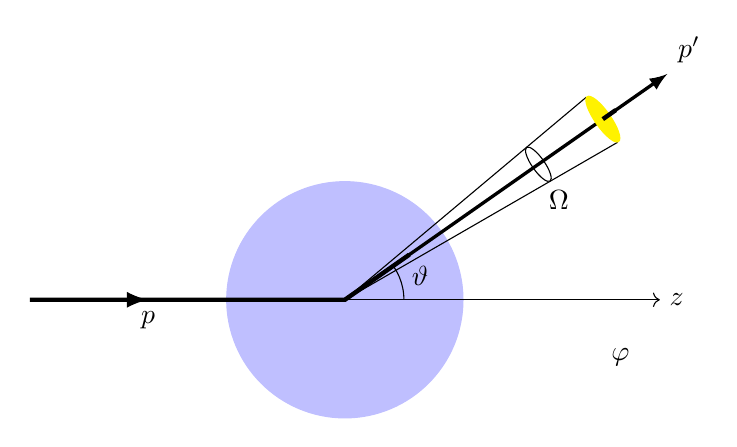
\begin{tikzpicture}
            \draw[fill=blue!25, draw=blue!25] (0, 0) circle [radius=1.5cm];
            \draw (0, 0) -- (30:4);
            \draw (0, 0) -- (40:4);
            \draw[->, >=latex, very thick] (0, 0) -- (35:5) node[above right] {\(\vv{p'}\)};
            \draw[fill=yellow, draw=yellow, rotate around={-55:(35:4)}] (35:4) circle[x radius=0.348cm, y radius=0.1cm];
            \draw[rotate around={-55:(35:3)}] (35:3) circle[x radius=0.261cm, y radius=0.08cm];
            \node at (25:3) {\(\dd{\Omega}\)};
            \draw[ultra thick] (35:4) -- (35:4.2);
            \draw[->, >=latex, ultra thick] (-4, 0) -- (-2.5, 0) node[below] {\(\vv{p}\)};
            \draw[ultra thick] (-4, 0) -- (0, 0) -- (35:1);
            \draw[->] (0, 0) -- (4, 0) node[right] {\(z\)};
            \begin{scope}[xscale=0.5]
                \centerarc[white, ultra thick](7, 0)(25:340:0.5)
                \centerarc[->](7, 0)(25:340:0.5)
            \end{scope}
            \node[below] at (3.5, -0.5) {\(\varphi\)};
            \begin{scope}
                \clip (0, 0) -- (4, 0) -- (35:4) -- cycle;
                \draw (0, 0) circle [radius=0.75cm];
            \end{scope}
            \node at (17.5:1) {\(\vartheta\)};
        \end{tikzpicture}
        \caption{A beam of particles with momentum \(\vv{p} = \hbar\vv{k}\) incident on a scattering centre at \(\vv{r} = 0\). We model this as a repulsive potential in the shaded area. The deflected beam has momentum \(\vv{p'} = \hbar\vv{k'}\) and intersects a detector of solid angle \(\dd{\Omega}\).}
        \label{fig:scattering setup}
    \end{figure}
    Figure~\ref{fig:scattering setup} shows the set up for a scattering experiment.
    A beam of particles with momentum \(\vv{p} = \hbar\vv{k}\) is incident on a scattering centre, which we define to be at the origin, \(\vv{r} = 0\).
    The beam is then scattered at an angle \(\vartheta\) and has momentum \(\vv{p'} = \hbar\vv{k'}\).
    The scattering process is characterised by two quantities:
    \begin{itemize}
        \item The incident flux, that is the number of incident particles crossing unit area perpendicular to the beam direction per unit time.
        This has dimensions of \([L]^{-2}[T]^{-1}\).
        \item The scattered flux, that is the number of scattered particles scattered into an element of solid angle \(\dd{\Omega}\) about the direction \(\vartheta, \varphi\) per unit time per unit solid angle.
        This has dimensions of \([T]^{-1}\).
    \end{itemize}
    We define the differential cross section as
    \[\dv{\sigma}{\Omega} = \frac{\text{scattered flux}}{\text{incident flux}}.\]
    This has dimensions of \([L]^2\) so is, as expected, an area.
    The total cross section is then found by integrating over all directions:
    \[\sigma_{T} = \int_{S^2} \dv{\sigma}{\Omega}\dd{\Omega} = \int_{0}^{2\pi}\int_{0}^{\pi} \dv{\sigma}{\Omega} \dd{\vartheta}\dd{\varphi}.\]
    Here \(S^2\) is the unit sphere.
    
    \subsection{The Born Approximation}
    If the interaction between the particle and the scattering centre is localised to the location of the scattering centre at \(\vv{r} = \vv{0}\) then we can consider the incoming particles as free (with momentum \(\vv{p}\) and when they reach the scattering centre they are in a potential which we can model as a constant perturbation.
    The particles are then scattered and become free again (with momentum \(\vv{p'}\).
    The Hamiltonian for the system is then
    \[\operator{H} = \operator{H}_0 + \operator{V}(\vv{r})\]
    where \(\operator{H}_0\) is the free Hamiltonian,
    \[\operator{H}_0 = \frac{\operator{p}^2}{2m}\]
    and \(\operator{V}(\vv{r})\) is the interaction potential that we treat as a perturbation inducing transitions between the eigenstates of \(\operator{H}_0\).
    
    It is better to work with the wave-vectors, \(\vv{k}\), than the momenta, \(\vv{p} = \hbar\vv{k}\).
    The transition rate is then
    \[R = \frac{2\pi}{\hbar} \abs{\bra{\vv{k'}} \operator{V} \ket{\vv{k}}} \rho(E_{k'})\]
    where \(\rho(E_{k'})\) is the density of final states which is defined such that \(\rho(E_{k'})\dd{E_{k'}}\) is the number of final states with energy in \([E_{k'}, E_{k'} + \dd{E_{k'}}]\).
    As usual
    \[V_{\vv{k'}\vv{k}} = \bra{\vv{k'}}\operator{V}\ket{\vv{k}} = \int u_{\vv{k'}}^*(\vv{r}) V(\vv{r}) u_{\vv{k}}(\vv{r}) \dd[3]{r}\]
    are the matrix elements of the operator \(\operator{V}\) in the momentum basis.
    
    \subsubsection{Technical Aside}
    The eigenstates of \(\operator{H}_{0}\) are plane waves of the form
    \[u_{\vv{k}}(\vv{r}) = C\exp(i\vv{k}\cdot\vv{r}) = C\exp(i\vv{p}\cdot\vv{r}/\hbar).\]
    The problem with this is that these are not properly normalisable as \(u\notin\squareIntegrable(\reals^3)\).
    The solution for this is to consider the system to be in a cubic box of side length \(L\).
    This solves the problem as \(u\in\squareIntegrable([-L/2, L/2]^3)\).
    We then take the limit as \(L \to \infty\).
    
    We can use therefore calculate the normalisation constant, \(C\), by requiring that
    \[1 = \int_{[-L/2, L/2]^{3}} u_{\vv{k}}^*(\vv{r}) u_{\vv{k}}(\vv{r}) \dd[3]{r} = \abs{C}^2 \int_{[-L/2, L/2]^3} \dd[3]{r} = \abs{C}^2L^3 \implies C = L^{-3/2},\]
    where we have used the fact that states are only defined up to a constant phase factor to choose \(C \in \reals_{\ge 0}\).
    Hence the properly normalised eigenstates are
    \[u_{\vv{k}}(\vv{r}) = L^{-3/2} \exp(i\vv{k}\cdot\vv{r}).\]
    We choose here to use periodic boundary conditions such that
    \[u(-L/2, y, z) = u(L/2, y, z)\]
    and similar in the \(y\) and \(z\) directions.
    The momentum eigenvalues are then
    \[\vv{p} = \hbar\vv{k} = \frac{2\pi\hbar}{L}(n_{x}, n_{y}, n_{z})\]
    where \(n_i \in \integers\).
    By choosing \(L\) to be very large we can approximate this as a continuous spectrum.
    
    \subsubsection{Density of Final States}
    \textit{For more detail on density of states see the statistical mechanics part of the thermal physics course.}
    
    Any wave vector \(\vv{k}\) can be viewed as a point in \(k\)-space with coordinates \((k_x, k_y, k_z)\).
    The allowed momentum states form a cubic lattice with spacing \(2\pi/L\).
    The density of states is the number of states per unit volume in \(k\)-space.
    In this case the density of states is \((L/2\pi)^3\).
    The number of states in a volume element of \(k\)-space, \(\dd[3]{k'}\), is
    \[\left( \frac{L}{2\pi} \right)^3 \dd[3]{k'} = \left( \frac{L}{2\pi} \right)^3 k'{^2} \dd{k'}\dd{\Omega}.\]
    We want to know the density of states per unit energy.
    We can do this using the following relationship as a transformation of variables:
    \[E_{k'} = \frac{\hbar^2 k'{^2}}{2m},\]
    which is the energy associated with a state of wave vector \(\vv{k'}\).
    We then have
    \[\rho(E_{k'})\dd{E_{k'}} = \left( \frac{L}{2\pi} \right)^3 k'{^2}\dd{k'}\dd{\Omega}\]
    which is the number of states with energy in \([E_{k'}, E_{k'} + \dd{E_{k'}}]\) or equivalently with wave vector in \([k'_{i}, k'_{i} + \dd{k'_i}]\).
    We can transform the differential using
    \[\dd{E_{k'}} = \abs{\dv{E_{k'}}{k'}}\dd{k'} = \frac{\hbar^2k'}{m}\dd{k'}.\]
    So we can identify \(\rho(E_{k'})\) as
    \[\rho(E_{k'}) = \frac{L^3mk'}{8\pi^3\hbar^2}\dd{\Omega}.\]
    
    \subsubsection{Incident Flux}
    By normalising the system in a box we have a system with a particle density of one particle per volume \(L^3\).
    This particle has a velocity \(\vv{v} = \vv{p}/m = \hbar\vv{k}/m\) and so the flux per unit area per unit time perpendicular to the beam is
    \[\text{incident flux} = \frac{\abs{\vv{v}}}{L^3} = \frac{\hbar k}{mL^3}.\]
    
    \subsubsection{Scattered Flux}
    The rate of transition between the initial state, \(\vv{k}\), and final state, \(\vv{k'}\), which corresponds to a wave vector pointing into the solid angle \(\dd{\Omega}\) about the direction \((\vartheta, \varphi)\), is given, via the golden rule, by
    \[R = \frac{2\pi}{\hbar} \abs{V_{\vv{k'}\vv{k}}}^2 \frac{L^3}{8\pi^3}\frac{mk'}{\hbar^2}\dd{\Omega}.\]
    This is the number of particles scattered into \(\dd{\Omega}\) per unit time.
    The flux is then given by dividing by \(\dd{\Omega}\):
    \[\text{scattered flux} = \frac{2\pi}{\hbar} \abs{V_{\vv{k'}\vv{k}}}^2 \frac{L^3}{8\pi^3}\frac{mk'}{\hbar^2}.\]
    
    \subsubsection{Differential Cross Section}
    The differential cross section is then
    \[\dv{\sigma}{\Omega} = \frac{\text{scattered flux}}{\text{incident flux}} = \frac{mL^3}{\hbar k}\frac{2\pi}{\hbar} \abs{V_{\vv{k'}\vv{k}}}^2 \frac{L^3}{8\pi^3} \frac{mk'}{\hbar^2}.\]
    For a real potential with elastic scattering we have \(k = k'\) and so we obtain the \define{Born approximation} of the differential cross section:
    \[\dv{\sigma}{\Omega} = \frac{m^2}{4\pi^2\hbar^4} L^6 \abs{\bra{\vv{k'}} \operator{V} \ket{\vv{k}}}^2\]
    where the matrix element is given by
    \[\bra{\vv{k'}}\operator{V}\ket{\vv{k}} = \frac{1}{L^3} \int V(\vv{r}) \exp(-i\vv{q}\cdot\vv{r}) \dd[3]{r}\]
    where \(\vv{q} = \vv{k'} - \vv{k}\) (sometimes also \(\vv{K}\)) is the \define{wave vector transfer}.
    The integral is over the entire box but we take \(L \to \infty\) such that the integral is over all space.
    Notice that this is simply the Fourier transform of the potential, \(V\).
    Also notice the factor of \(L^{-3}\) so that in the resulting differential cross section the explicit \(L\) dependence cancels out.
    
    \section{Central Potentials and Two Body Scattering}
    A central potential is of the form \(V(\vv{r}) = V(r)\), meaning it is spherically symmetric.
    This allows us to simplify the Born approximation by partly evaluating the matrix element using this symmetry.
    To do this we work in a spherical polar system with coordinates \((K, \Theta, \Phi)\) where \(\vv{K} = (K, 0, 0) = \vv{k'} - \vv{k}\) is the wave transfer vector.
    This means that \(\vv{K}\cdot\vv{r} = Kr\cos\Theta\).
    Considering the integral defining the matrix element we have
    \begin{align*}
        \bra{\vv{k'}} \operator{V} \ket{\vv{k}} &= \int V(r) \exp(-i\vv{K}\cdot\vv{r}) \dd[3]{r}\\
        &= \int_{0}^{2\pi} \dd{\Phi} \int_{0}^{\pi} \dd{\Theta} \int_{0}^{\infty} \dd{r} r^2 \sin\Theta V(r) \exp(-iKr\cos\Theta)\\
        &= 2\pi \int_{-1}^{1} \int_{0}^{\infty} r^2 V(r) \exp(-iKr\cos\Theta) \dd{r} \dd{(\cos\Theta)}\\
        &= 2\pi \int_{0}^{\infty} r^2V(r) \left[ \frac{\exp(-iKr\cos\Theta)}{-iKr} \right]_{-1}^{1} \dd{r}\\
        &= 2\pi \int_{0}^{\infty } rV(r) \left[ \frac{\exp(-iKr) - \exp(iKr)}{iK} \right] \dd{r}\\
        &= \frac{4\pi}{K} \int_{0}^{\infty} r V(r) \sin(K r) \dd{r}.
    \end{align*}
    Here we have used a trick substituting for \(\cos\Theta\), see appendix~\ref{app:cos theta substitution} for more details.
    The Born approximation for a central potential is then
    \[\dv{\sigma}{\Omega} = \frac{4m^2}{\hbar^4K^2} \abs{\int_{0}^{\infty} rV(r) \sin(Kr) \dd{r}}^2.\]
    Notice that this is independent of \(\varphi\) as the system is rotationally symmetric about the \(z\) axis but depends on \(\vartheta\) through the direction of \(\vv{K}\).
    We can write this result in terms of the spherical coordinate system \((k, \vartheta, \varphi)\) which has its polar axis aligned with the incoming beam.
    We simply need a bit of trigonometry and the fact that \(k = k'\).
    Then it can be seen from figure~\ref{fig:geometry of elastic scattering} that
    \[K = 2k\sin\frac{\vartheta}{2}.\]
    \begin{figure}[ht]
        \centering
        \tikzsetnextfilename{geometry-of-elastic-scattering}
        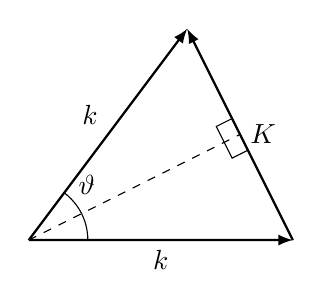
\begin{tikzpicture}[rotate={atan(0.5)}, scale=1.5]
            \draw[->, >=latex, thick] (0, 0) -- (2, 1) node[above left, midway] {\(\vv{k}\)};
            \draw[->, >=latex, thick] (0, 0) -- (2, -1) node[below, midway] {\(\vv{k}\)};
            \draw[->, >=latex, thick] (2, -1) -- (2, 1) node[right, midway] {\(\vv{K}\)};
            \draw[dashed] (0, 0) -- (2, 0);
            \draw (2, -0.15) rectangle (1.85, 0.15);
            \begin{scope}
                \clip (0, 0) -- (2, 1) -- (2, -1) -- cycle;
                \draw (0, 0) circle[radius=0.5cm];
            \end{scope}
            \node at (0.65, 0.2) {\(\vartheta\)};
        \end{tikzpicture}
        \caption{The relationship between wave vectors with elastic scattering, \(k = k'\).}
        \label{fig:geometry of elastic scattering}
    \end{figure}
    \subsection{Screened Coulomb Potential}
    The classical Coulomb potential is not local and therefore we cannot use the Born approximation.
    However suppose we consider an incoming electron scattering off of an atom.
    The atomic electrons provide screening which we model as a \define{screening factor} \(\exp(-\beta r)\) for some constant \(\beta > 0\).
    Thus the potential has the form
    \[V(r) = -\frac{Ze^2}{4\pi\varepsilon_0r} e^{-\beta r}.\]
    This is a central potential and so
    \begin{align*}
        \frac{K}{4\pi} \bra{\vv{k'}} \operator{V} \ket{\vv{k}} &= \int_{0}^{\infty} rV(r) \sin(Kr)\dd{r}\\
        &= -\frac{Ze^2}{4\pi\varepsilon_0} \int_{0}^{\infty} e^{-\beta r}\sin(Kr)\dd{r}\\
        &= -\frac{Ze^2}{4\pi\varepsilon_0} \int_{0}^{\infty} e^{-\beta r}\frac{1}{2i}[e^{iKr} - e^{-iKr}]\dd{r}\\
        &= -\frac{Ze^2}{4\pi\varepsilon_0} \frac{1}{2i} \int_{0}^{\infty} [e^{(iK - \beta)r} - e^{-(iK + \beta)r}\dd{r}\\
        &= -\frac{Ze^2}{4\pi\varepsilon_0} \frac{1}{2i} \left[ \frac{\exp[(iK - \beta)r]}{iK - \beta} + \frac{\exp[-(iK + \beta)]}{iK + \beta} \right]_{0}^{\infty}\\
        &= -\frac{Ze^2}{4\pi\varepsilon_0} \frac{1}{2i} \left[ \frac{1}{iK - \beta} + \frac{1}{iK + \beta} \right]_{0}^{\infty}\\
        &= \frac{Ze^2}{4\pi\varepsilon_0} \frac{K}{\beta^2 + K^2}.
    \end{align*}
    Substituting this into the Born approximation we have
    \[\dv{\sigma}{\Omega} = \frac{4m^2}{\hbar^4 K^2}\left( \frac{Ze^2}{4\pi\varepsilon_0} \right)^2 \frac{K^2}{(\beta^2 + K^2)^2} = \frac{4m^2}{\hbar^4} \left( \frac{Ze^2}{4\pi\varepsilon} \right)^2 \frac{1}{(\beta^2 + K^2)^2}.\]
    This can then be further simplified if needed using
    \[K = 2k\sin\frac{\vartheta}{2} = \frac{2mv}{\hbar}\sin\frac{\vartheta}{2}.\]
    
    \subsubsection{Coulomb Scattering}
    We can obtain the cross section for scattering by an unscreened Coulomb potential by taking the limit \(\beta \to 0\).
    We then have
    \[\dv{\sigma}{\Omega} = \left( \frac{Ze^2}{4\pi\varepsilon_0} \right)^2 \frac{4m^2}{\hbar^4K^4} = \left( \frac{Ze^2}{4\pi\varepsilon_0} \right)^2 \frac{1}{4m^2v^4 \sin^4(\vartheta/2)}.\]
    This is the \define{Rutherford scattering cross section}.
    This result is identical to the classical result derived by Rutherford, it is essentially a fluke that the classical approximation by Rutherford and the quantum Born approximation both reduce to the same result.
    
    \subsection{Two Body Scattering}
    So far we have considered a particle (or beam of particles) scattering off a fixed scattering centre.
    A more realistic set up allows the scattering centre to move.
    This allows us to model events such as two incident particles colliding and scattering as one might see in an accelerator.
    Let \(\vv{r_i}\) and \(m_i\) be the position and mass of the \(i\)th particle and let \(\grad_i\) be the gradient operator that acts on the position of the \(i\)th particle.
    Then the Hamiltonian for a two particle scattering system is
    \[\operator{H} = - \frac{\hbar^2}{2m_1} \grad_1^2 - \frac{\hbar^2}{2m_2} \grad_2^2 + V(\vv{r_1} - \vv{r_2}).\]
    As with a classical two body system it is easiest to work in the \gls{cm} frame.
    We define
    \[\vv{R} = \frac{m_1\vv{r_1} + m_2\vv{r_2}}{m_1 + m_2}, \qquad\text{and}\qquad \vv{r} = \vv{r_1} - \vv{r_2},\]
    which are the centre-of-mass and relative position vectors respectively.
    Rearranging these definitions we can recover our initial coordinate systems:
    \[\vv{r_1} = \vv{R} + \frac{m_2}{m_1 + m_2}\vv{r}, \qquad \text{and}\qquad \vv{r_2} = \vv{R} - \frac{m_1}{m_1 + m_2} \vv{r}.\]
    We also need to express the gradient operators in this new system.
    Let \(x_j^{i}\), \(X_j\), and \(x_j\) be the components of \(\vv{r_i}\), \(\vv{R}\), and \(\vv{r}\) respectively.
    Then we can rewrite the derivatives as
    \[\pdv{x^i} = \pdv{X}{x_i}\pdv{X} + \pdv{x}{x^1}\pdv{x} = \frac{m_1}{m_1 + m_2}\pdv{X} + \pdv{x},\]
    and similarly for the two other directions.
    The Hamiltonian can then be written as
    \[\operator{H} = -\frac{\hbar^2}{2M}\grad_{R}^2 - \frac{\hbar^2}{2\mu} + V(\vv{r})\]
    where \(\grad_R\) and \(\grad\) are the gradient operators with respect to \(\vv{R}\) and \(\vv{r}\) respectively.
    Here \(M = m_1 + m_2\) is the combined mass and \(\mu = m_1m_2/(m_1 + m_2)\) is the reduced mass.
    
    We can separate this Hamiltonian into two parts:
    \[\operator{H} = \operator{H}_{\mathrm{CM}} + \operator{H}_{\mathrm{rel}}.\]
    The first of these,
    \[\operator{H}_{\mathrm{CM}} = -\frac{\hbar^2}{2M}\grad_R^2\]
    describes the motion of the centre of mass, which is free to move.
    In the \gls{cm} frame the centre of mass is, by definition, at rest and so the Hamiltonian reduces to
    \[\operator{H}_{\mathrm{rel}} = -\frac{\hbar^2}{2\mu}\laplacian + V(\vv{r}).\]
    This is the same as the Hamiltonian for a single particle at position \(\vv{r}\) in potential \(V\).
    Therefore we can obtain the differential cross section in the centre of mass frame in the same way we do for a single particle scattering off a fixed scattering centre.
    
    \section{Bonding in the \texorpdfstring{\ce{H_2^+}}{H2+} Ion}
    The simplest example of covalent bonding is the \ce{H_2^+} ion which consists of just three particles, two protons which share a single electron.
    This system has three terms in the potential, the two potentials between the electron and each proton and the potential between the two protons.
    We work in the \gls{cm} frame of the two protons (assuming the position of the electron has negligible effect on the centre of mass).
    See figure~\ref{fig:H2+ ion} for more details.
    \begin{figure}[ht]
        \centering
        \tikzsetnextfilename{H2+-ion}
        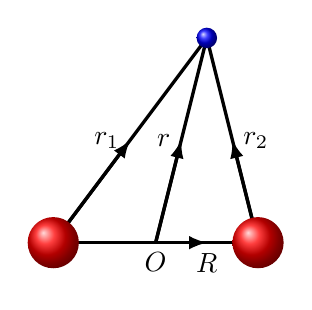
\begin{tikzpicture}[scale=1.3]
            \tikzset{vec/.style={very thick}}
            \coordinate (p1) at  (-1, 0);
            \coordinate (p2) at (1, 0);
            \coordinate (e) at (0.5, 2);
            \draw[vec] (p1) -- (e);
            \draw[vec, ->, >=latex] (p1) -- ($(p1)!0.5!(e)$) node[left] {\(\vv{r_1}\)};
            \draw[vec] (p2) -- (e);
            \draw[vec, ->, >=latex] (p2) -- ($(p2)!0.5!(e)$) node[right] {\(\vv{r_2}\)};
            \draw[vec] (0, 0) -- (e);
            \draw[vec, ->, >=latex] (0, 0) -- ($(0, 0)!0.5!(e)$) node[left] {\(\vv{r}\)};
            \draw[vec] (p1) -- (p2);
            \draw[vec, ->, >=latex] (p1) -- ($(p1)!0.75!(p2)$) node[below] {\(\vv{R}\)};
            \node[below] at (0, 0) {\(O\)};
            \draw[draw=none, ball color=red] (p1) circle[radius=0.25cm];
            \draw[draw=none, ball color=red] (p2) circle[radius=0.25cm];
            \draw[draw=none, ball color=blue] (e) circle[radius=0.1cm];
        \end{tikzpicture}
        \caption{The \ce{H_2^+} ion with centre of mass frame origin, \(O\), and proton separation \(\vv{R}\).}
        \label{fig:H2+ ion}
    \end{figure}
    
    The Schr\"odinger equation for this system is
    \[\left[ -\frac{\hbar^2}{2\mu_{12}}\grad_R^2 - \frac{\hbar^2}{2\mu_{\Pe}}\grad_r^2 - \frac{e^2}{4\pi\varepsilon_0r_1} - \frac{e^2}{4\pi\varepsilon_0r_2} + \frac{e^2}{4\pi\varepsilon_0R} \right] \psi(\vv{r}, \vv{R}) = E\psi(\vv{r}, \vv{R})\]
    where \(\mu_{12} = m_{\Pp}/2\) is the reduced proton mass, \(m_{\Pp}\) is the proton mass,
    \[\mu_{\Pe} = \frac{2m_{\Pp}m_{\Pe}}{2m_{\Pp} + m_{\Pe}} \approx m_{\Pe}\]
    is the reduced mass of the entire system and \(m_{\Pe}\) is the mass of an electron.
    
    \subsection{Born--Oppenheimer Approximation}
    Since protons are significantly more massive than electrons the motion of the nuclei is much slower than the motion of the electrons.
    We treat the nuclear and electronic motions as independent and when considering the electronic motion we consider the nuclei to be fixed.
    That is for each value of \(\vv{R}\) we can find a solution to the Schr\"odinger equation.
    
    The electron, in this approximation, is described by the state \(U_j(\vv{r}, \vv{R})\) which satisfies the Schr\"odinger equation
    \[\left[ -\frac{\hbar^2}{2\mu_{\Pe}}\grad_r^2 - \frac{e^2}{4\pi\varepsilon_0r_1} - \frac{e^2}{4\pi\varepsilon_0r_2} + \frac{e^2}{4\pi\varepsilon_0R} \right]U_j(\vv{r}, \vv{R}) = E_j(\vv{R})U_j(\vv{r}, \vv{R}).\]
    We can solve this for a given fixed \(\vv{R}\).
    For each value of \(\vv{R}\) we find a set of energy eigenvalues, \(E_j(\vv{R})\), and eigenfunctions, \(U_j(\vv{r}, \vv{R})\) which are the \define{molecular orbitals}.
    
    We then assume that the \(j\)th state is given by
    \[\psi(\vv{r}, \vv{R}) = F_j(\vv{R})U_j(\vv{r}, \vv{R})\]
    where \(F_j\) is a wave function describing the nuclear motion which is independent of the location of the electron.
    We can substitute this into the full Schr\"odinger equation and simplify further using the Schr\"odinger equation for electronic motion to get
    \[\left[ -\frac{\hbar^2}{2\mu_{12}}\grad_R^2 + E_j(\vv{R}) - E \right]F_j(\vv{R})U_j(\vv{r}, \vv{R}) = 0.\]
    Using some vector calculus identities we have
    \begin{align*}
        \grad_{R}^2[F_j(\vv{R}) U_j(\vv{r}, \vv{R})] &= \grad_R \cdot [\grad_R (F_j(\vv{R})U_j(\vv{r}, \vv{R}))]\\
        &= \grad_R \cdot [U_j(\vv{r}, \vv{R}) \grad_R F_j(\vv{R}) + F_j(\vv{R})\grad_R U_j(\vv{r}, \vv{R})]\\
        &= U_j(\vv{r}, \vv{R})\grad_R^2F_j(\vv{R}) + F_j(\vv{R})\grad_R^2U_j(\vv{r}, \vv{R}) + 2 [\grad_RU_j(\vv{r}, \vv{R})]\cdot[\grad_RF_j(\vv{R})].
    \end{align*}
    Assuming that the molecular orbitals, \(U_j\), don't change much with inter-nuclear separation, \(\vv{R}\), we neglect the terms including \(\grad_RU_j(\vv{r}, \vv{R})\) and \(\grad_R^2U_j(\vv{r}, \vv{R})\) and we are left with the Schr\"odinger equation
    \[\left[ -\frac{\hbar^2}{2\mu_{12}}\grad_R^2 + E_j(\vv{R}) - E \right]F_j(\vv{R}) = 0.\]
    This is the Schr\"odinger equation for a single particle of mass \(\mu_{12}\) in the potential \(E_j(\vv{R})\).
    
    \subsection{Electronic Ground State}
    We can find the lowest electronic energy levels of \ce{H_2^+} using the Rayleigh--Ritz variational method.
    First we notice that we can write \(\vv{r_1} = \vv{r} + \vv{R}/2\) and \(\vv{r_2} = \vv{r} - \vv{R}/2\).
    This means that under the parity operator, \(\operator{\parity}\), defined by \(\operator{\parity}f(\vv{r}) = f(-\vv{r})\) we have \(\operator{\parity}\vv{r_1} = -\vv{r_2}\) and \(\operator{\parity}\vv{r_2} = -\vv{r_1}\) so by relabelling \(1 \leftrightarrow 2\) the Hamiltonian is invariant under \(\operator{\parity}\).
    This means that
    \[[\operator{\parity}, \operator{H}] = 0.\]
    The compatibility theorem then tells us that \(\operator{\parity}\) and \(\operator{H}\) have a simultaneous eigenbasis.
    As eigenfunctions of \(\operator{\parity}\) these must be either even, in which case we call them \textit{gerade} or \(\gerade\), or odd, in which case we call them \textit{ungerade} or \(\ungerade\)\footnote{\textit{gerade} and \textit{ungerade} are German for even and odd respectively}.
    So we can split the eigenfunctions into two types based on their parity:
    \[\operator{\parity}U_j^{\gerade}(\vv{r}, \vv{R}) = U_{j}^{\gerade}(\vv{r}, \vv{R}), \qquad \text{and} \qquad \operator{\parity}U_j^{\ungerade}(\vv{r}, \vv{R}) = -U_j^{\ungerade}(\vv{r}, \vv{R}).\]
    We now need to come up with a trial function, or in this case two trial functions for \textit{gerade} and \textit{ungerade} eigenfunctions.
    Suppose \(\vv{R}\) is very large.
    Then the system approximates a free proton and a hydrogen atom.
    This suggests that the hydrogen atom eigenfunctions may make good trial functions.
    We are interested in the ground state so we use the \(1\mathrm{s}\) eigenstates, which are even, to construct the trial states
    \[\psi^{\gerade} = u_{1\mathrm{s}}(r_1) + u_{1\mathrm{s}}(r_2), \qquad\text{and}\qquad \psi^{\ungerade} = u_{1\mathrm{s}}(r_1) - u_{1\mathrm{s}}(r_2).\]
    This procedure, is known as taking \gls{lcao}.
    We can calculate the expectation value of the electronic Hamiltonian using these trial wave functions:
    \[E^{\gerade,\ungerade}(\vv{R}) = \frac{\int \psi^{\gerade,\ungerade}{^*}(\vv{r}, \vv{R})\operator{H}\psi^{\gerade,\ungerade}(\vv{r}, \vv{R})\dd[3]{r}}{\int \abs{\psi^{\gerade,\ungerade}(\vv{r}, \vv{R})}^2\dd[3]{r}}.\]
    This gives an upper bound on the energies, \(E^{\gerade}(\vv{R})\) and \(E^{\ungerade}(\vv{R})\), for a given value of \(\vv{R}\).
    We treat \(\vv{R}\) here as a variational parameter.
    
    Evaluating these integrals is complicated and not very informative so we simply state the solutions:
    \begin{align*}
        E^{\gerade}(\vv{R}) &= E_{1\mathrm{s}} + \frac{e^2}{4\pi\varepsilon_0R} \frac{(1 + R/a_0)e^{-2R/a_0} + [1 - \tfrac{2}{3}(R/a_0)^2]e^{-R/a_0}}{1 + [1 + R/a_0 + \tfrac{1}{3}(R/a_0)^2]e^{-R/a_0}},\\
        E^{\ungerade}(\vv{R}) &= E_{1\mathrm{s}} + \frac{e^2}{4\pi\varepsilon_0R} \frac{(1 + R/a_0)e^{-2R/a_0} - [1 - \tfrac{2}{3}(R/a_0)^2]e^{-R/a_0}}{1 + [1 + R/a_0 + \tfrac{1}{3}(R/a_0)^2]e^{-R/a_0}}.
    \end{align*}
    Here \(a_0 = \SI{5.29e-11}{\metre}\) is the Bohr radius and \(E_{1\mathrm{s}} = \SI{13.6}{\electronvolt}\) is the ground state energy of atomic hydrogen.
    To fully apply the variational method we need to find \(\vv{R}\) such that these energies are minimised.
    If we do this then we find that the even orbital has a minimum at \(R = R_0 \approx 2.5a_0\) which corresponds to \(E^{\gerade} - E_{1\mathrm{s}} = -\SI{1.77}{\electronvolt}\).
    This is an upper bound on the ground state energy and so we conclude that there is a stable bound state, which of course we know to be the case.
    In contrast there is no minimum for \(E^{\ungerade}\) so any \ce{H_2^+} ion in an antisymmetric-state will dissociate into a proton and a hydrogen atom.
    
    This makes sense as we can think of the even states as more tightly bound because the wave function peaks in between the protons and therefore provides shielding and more tightly bonds the ion together.
    On the other hand the odd wave function vanishes directly between the two protons and therefore the antisymmetric system is less tightly bound.
    
    \begin{figure}[ht]
        \centering
        \tikzsetnextfilename{energy-levels-H-2-plus-ion}
        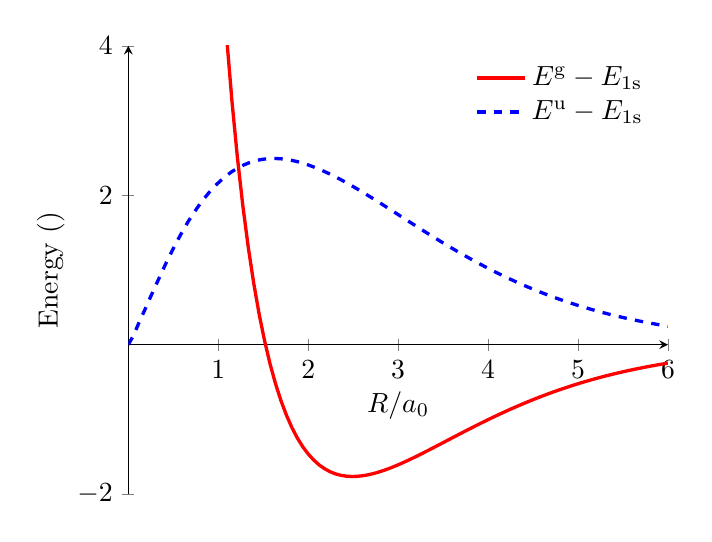
\begin{tikzpicture}
            \pgfmathsetmacro{\prefactor}{27.2113862}  % prefactor, e^2/(4 pi epsilon0 a0) in electron volts
            \begin{axis}[
                domain=0:6,
                ymax=4,
                ymin=-2,
                axis lines=middle,
                legend style={draw=none},
                xlabel={\(R/a_0\)},
                ylabel={Energy (\si{\electronvolt})},
                x label style={at={(axis description cs:0.5,0.25)},anchor=north},
                y label style={at={(axis description cs:-0.1,.5)},rotate=90,anchor=south}
                ]
                \addplot[
                samples=100,
                very thick,
                red
                ]
                {\prefactor * ((1 + x) * e^(-2*x) + (1 - 2*x^2/3) * e^(-x))/(x + x * (1 + x + x^2/3) * e^(-x))};
                \addlegendentry{\(E^\gerade - E_{1\mathrm{s}}\)}
                
                \addplot [
                samples=100,
                very thick,
                blue,
                dashed
                ]
                {\prefactor * ((1 + x) * e^(-2*x) - (1 - 2*x^2/3) * e^(-x))/(x + x * (1 + x + x^2/3) * e^(-x))};
                \addlegendentry{\(E^\ungerade - E_{1\mathrm{s}}\)}
            \end{axis}
        \end{tikzpicture}
        \caption{Plot of \(E^{\gerade} - E_{1\mathrm{s}}\) as a function of inter--nuclear separation, \(R/a_0\).}
    \end{figure}
    
    %%%%%%%%%%%%%%%%%%%%%%%%%%%%%%%%%%%%%%%%%%%%%%%%%%%%%%%%%%%%%%%%%%%%
    \tikzexternaldisable
    %%%%%%%%%%%%%%%%%%%%%%%%%%%%%%%%%%%%%%%%%%%%%%%%%%%%%%%%%%%%%%%%%%%%
    
    \subsection{Rotational and Vibrational Modes}
    We can now consider the effective one body Schr\"odinger equation for the electronic ground state \(E_j(\vv{R}) = E^{\gerade}(\vv{R})\).
    Since \(E^{\gerade}(R)\) depends only on the magnitude of \(\vv{R}\) this corresponds to an effective central potential.
    Therefore the solutions are of the form
    \[F^{\gerade}(\vv{R}) = \frac{1}{R}\mathcal{R}_{NL}(R)Y_{L}^{M_L}(\vartheta, \varphi)\]
    where \(\mathcal{R}_{NL}\) satisfies
    \[\left[ -\frac{\hbar^2}{2\mu_{12}}\left( \dv[2]{R} - \frac{L(L + 1)}{R^2} \right) + E^{\gerade}(\vv{R}) - E \right]\mathcal{R}_{NL}(R) = 0.\]
    We can Taylor expand \(E^{\gerade}\) about \(R = R_0\).
    Since this is a minimum the first order term vanishes:
    \[E^{\gerade}(R) \approx E^{\gerade}(R) + \frac{1}{2}k(R - R_0)^2 + \dotsb\]
    where \(k = E^{\gerade}{''}(R_0)\).
    We can also define
    \[E_r = \frac{\hbar^2}{2\mu_{12}R_0}L(L + 1)\]
    which gives the value of the centrifugal barrier (the second term in the Hamiltonian) at the point \(R = R_0\).
    Using this to approximate the centrifugal term and the Taylor series to approximate the potential we have
    \[\left[ -\frac{\hbar^2}{2\mu_{12}}\dv[2] + \frac{1}{2}k(R - R_0)^2 - E_N \right]\mathcal{R}_{NL}(R) = 0\]
    where we combine all energy terms into one:
    \[E_N = E - E^{\gerade}(R_0) - E_r.\]
    We can now identify this Schr\"odinger equation as corresponding to a harmonic oscillator which has energy levels
    \[E_N = \hbar\omega_0\left( N + \frac{1}{2} \right)\]
    for \(N = 0, 1, 2, \dotsc\) and \(\omega_0 = \sqrt{k/\mu_{12}}\).
    
    The vibrational modes (which correspond to \(E_N\)) are on the order of \(\SI{0.1}{\electronvolt}\) (which corresponds to \(T = \SI{1160}{\kelvin}\)).
    It is also possible to compute the rotational modes which are on the order of \(\SI{0.001}{\electronvolt}\) (which corresponds to \(T = \SI{11.6}{\kelvin}\)).
    Both of these are much smaller than the spacing between electronic energy levels, which are on the order of \(\SI{1}{\electronvolt}\) (which corresponds to \(\SI{11600}{\kelvin}\).
    Notice that at room temperature it is possible to reach the rotational but not vibrational modes which is a fact we rely on in thermodynamics.
    The electronic energy level separations lead to molecular absorption/emission spectra and zooming in on a given line we see a vibrational--rotational spectra.
    
    \clearpage
    \appendix
    \part*{Appendix}
    \addcontentsline{toc}{part}{Appendix}
    \begingroup
    \section{Algebraic Structures}
    In section~\ref{sec:vector spaces} we discussed vector spaces.
    We defined a vector space, \(\hilbert\), over a field, \(\mathbb{F}\).
    But what is a field?
    Intuitively a field is a set with addition, multiplication, subtraction, and division defined as we would expect.
    To be more rigorous we need a couple of definitions first.
    
    \subsection{Groups}
    A \define{group}, \((G, \circ)\), is a set, \(G\), along with a binary operation 
    \begin{align*}
        \circ\colon G\times G &\to G\\
        x, y &\mapsto x\circ y = z\in G.
    \end{align*}
    This binary operation satisfies the following:
    \begin{itemize}
        \item Associativity -- For all \(x, y, z\in G\) we have
        \[x \circ (y \circ z) = (x \circ y) \circ z.\]
        \item Identity -- There exists \(e\in G\) such that for all \(x\in G\) we have
        \[e \circ x = x \circ e = x.\]
        \(e\) is called the identity.
        \item Inverse -- For all \(x\in G\) there exists \(x^{-1}\in G\) such that
        \[x \circ x^{-1} = x^{-1} \circ x = e\]
        where \(e\) is the identity.
    \end{itemize}
    An example of a group is the group of all permutations, \(\sigma\colon \{1, \dotsc, n\} \to \{1, \dotsc, n\}\) such that \(\sigma\) is a bijection.
    Here the group operation is function composition.
    
    If \((G, \circ)\) is a group and for all \(x, y\in G\) we have
    \[x\circ y = y\circ x\]
    then we say \((G, \circ)\) is an \define{abelian group}.
    An example of an abelian group is \(\integers_2 = \{0, 1\}\) under addition modulo 2.
    
    \subsection{Rings}
    A \define{ring}, \((R, +, \cdot)\), is a set, \(R\), along with two binary operations:
    \begin{align*}
        +\colon R\times R &\to R\\
        x, y &\mapsto x + y = z\in R,
    \end{align*}
    which we call addition, and
    \begin{align*}
        \cdot\colon R\times R &\to R\\
        x, y &\mapsto xy = z'\in R,
    \end{align*}
    which we call multiplication.
    These two operations satisfy the following:
    \begin{itemize}
        \item \((R, +)\) is an abelian group.
        \item Associativity of multiplication -- For all \(x, y, z\in R\)
        \[x(yz) = (xy)z.\]
        \item Distributivity of multiplication over addition -- For all \(x, y, z\in R\)
        \[x(y + z) = xy + xz,\qquad\text{and}\qquad (x + y)z = xz + yz.\]
    \end{itemize}
    We denote the identity of \((R, +)\) by \(0\) and inverses of addition as \(-x\) (as opposed to \(x^{-1}\)).
    An example of a ring is \(M_2(2\integers)\), which is the set of \(2\times 2\) matrices with entries from \(2\integers = \{0, \pm 2, \pm 4, \pm 6, \dotsc\}\).
    Here the operations are matrix addition and matrix multiplication.
    
    
    If \(R\) is a ring (we drop the \(+\) and \(\cdot\) for brevity) and there exists \(1\in R\) such that \(1x = x1 = x\) for all \(x\in R\) then \(R\) is a \define{ring with unity}.
    An example of a ring with unity is \(M_2(\integers)\) which is the set of all \(2\times 2\) matrices with entries from \(\integers\), in this case the identity matrix plays the role of the multiplicative identity.
    
    If \(R\) is a ring with unity and for all \(x\in R\) such that \(x\ne 0\) there exists \(x^{-1}\in R\) such that \(xx^{-1} = x^{-1}x = 1\) then \(R\) is a \define{division ring}.
    An example of a ring with unity is the quaternions, \(\quaternions\), with quaternion addition and multiplication.
    
    If \(R\) is a ring and for all \(x, y\in R\) we have \(xy = yx\) then \(R\) is a \define{commutative ring}.
    An example of a commutative ring is \(2\integers\) with normal integer addition and multiplication.
    
    
    If \(R\) is a commutative ring and for all \(a, b\in R\) we have \(ab = 0\) if and only if \(a = 0\) and/or \(b = 0\) then \(R\) is an \define{integral domain}.
    An example of an integral domain is \(\integers\) with normal integer addition and multiplication.
    
    If \(R\) is a commutative division ring, and \(1\ne 0\), then it is a \define{field}.
    Examples of fields includes \(\rationals\), \(\reals\), and \(\complex\), with their respective addition and multiplication operations.
    As well as these \(\integers_p = \{0, \dotsc, p-1\}\) for prime \(p\) under addition and multiplication modulo \(p\) is a field.

    \section{Sum of \texorpdfstring{\(k\)}{k} From 0 to \texorpdfstring{\(n\)}{n} Proof}\label{sec:proof sum 0 to n of r is 0.5 n(n+1)}
    \begin{theorem}{}{}
        For \(n \in \naturals\)
        \[\sum_{r=0}^{n} r = \frac{1}{2}n(n + 1).\]
    \end{theorem}
    \begin{proof}
        We will prove this by induction.
        First note that
        \[\sum_{r=0}^{0}r\]
        is the empty sum which is defined to be zero by convention.
        Now suppose that this result holds for some \(k \in \naturals\), that is
        \[\sum_{r = 0}^{k} r = \frac{1}{2}k(k + 1).\]
        Then
        \begin{align*}
            \sum_{r = 0}^{k + 1} r &= \sum_{r = 0}^{k} r + (k + 1)\\
            &= \frac{1}{2}k(k + 1) + (k + 1)\\
            &= (k + 1)\left[\frac{1}{2}k + 1\right]\\
            &= \frac{1}{2}(k + 1)(k + 2)
        \end{align*}
        which is exactly what we would expect if the hypothesis held for \(k + 1\).
        Hence by induction
        \[\sum_{r=0}^{n} r = \frac{1}{2}n(n + 1)\]
        holds for all \(n\in\naturals\).
    \end{proof}
    \section{Clebsch--Gordan Coefficients}
    The Clebsch--Gordan coefficients are, using the notation of section~\ref{sec:addition of angular momenta}, the coefficients
    \[\braket{j_1, m_1, j_2, m_2}{j, m; j_1, j_2}\]
    in the transformation from the uncoupled to coupled basis:
    \[\ket{j, m; j_1, j_2} = \sum_{m_1 = -j_1}^{j_1}\sum_{m_2 = -j_2}^{j_2} \braket{j_1, m_1, j_2, m_2}{j, m; j_1, j_2} \ket{j_1, m_1, j_2, m_2}.\]
    There is an explicit solution to this, namely
    \begin{align*}
        \braket{j_1, m_1, j_2, m_2}{j, m; j_1, j_2} &= \delta_{m,m_1+m_2} \sqrt{\frac{(2j + 1)(j + j_1 - j_2)!(j - j_1 + j_2)!(j_1 + j_2 - j)!}{(j_1 + j_2 + j + 1)!}} \times\\
        &\qquad \sqrt{(j + m)!(j - m)!(j_1 - m_1)!(j_1 + m_1)!(j_2 - m_2)!(j_2 + m_2)!} \times\\
        &\qquad \sum_k \left[\sqrt{\frac{(-1)^k}{k!(j_1 + j_2 - j - k)!(j_1 - m_1 - k)!(j_2 + m_2 - k)!}}\right.\times\\
        &\qquad\qquad \left.\sqrt{\frac{1}{(j - j_2 + m_1 + k)!(j - j_1 - m_2 + k)!}}\,\,\right].
    \end{align*}
    The summation is over all \(k\in\integers\) such that the argument of every factorial is non-negative.
    Solutions with \(m < 0\) or \(j_1 < j_2\) have been omitted.
    Solutions with \(m < 0\) can be found using the relation
    \[\braket{j_1, m_1, j_2, m_2}{j, m; j_1, j_2} = (-1)^{j - j_1 - j_2}\braket{j_1, m_2, j_2, m_2}{j, -m, j_1, j_2}\]
    and solutions with \(j_1 < j_2\) can be found using the relation
    \[\braket{j_1, m_1, j_2, m_2}{j, m; j_1, j_2} = (-1)^{j - j_1 - j_2}\braket{j_2, m_2, j_1, m_2}{j, m; j_2, j_1}.\]
    
    Clearly this is impractical to use every time.
    The common thing to do is to pre-calculate values or use a computer.
    Some pre-calculated values are given here.
    \subsection{Pre-Calculated Clebsch--Gordan Coefficients}
    When \(j_2 = 0\)  the Clebsch--Gordan coefficients are given by \(\delta_{jj_1}\delta_{mm_1}\).
    
    \begin{table}[ht]
        \centering
        \begin{subtable}{0.25\textwidth}
            \centering
            \begin{tabular}{|l|l|}\hline
                \backslashbox{\(m_1, m_2\)}{\(j\)} & 1\\ \hline
                \(1/2, 1/2\) & 1\\ \hline
            \end{tabular}
            \subcaption{\(m = 1\)}
        \end{subtable}
        \begin{subtable}{0.25\textwidth}
            \centering
            \begin{tabular}{|l|l|}\hline
                \backslashbox{\(m_1, m_2\)}{\(j\)} & 1\\ \hline
                \(-1/2, -1/2\) & 1\\ \hline
            \end{tabular}
            \subcaption{\(m = -1\)}
        \end{subtable}
        \begin{subtable}{0.4\textwidth}
            \centering
            \begin{tabular}{|l|l|l|}\hline
                \backslashbox{\(m_1, m_2\)}{\(j\)} & 1 & 0\\ \hline
                &&\\[-1em]
                \(1/2, -1/2\) & \(\sqrt{1/2}\) & \(\sqrt{1/2}\)\\ \hline
                &&\\[-1em]
                \(-1/2, 1/2\) & \(\sqrt{1/2}\) & -\(\sqrt{1/2}\)\\ \hline
            \end{tabular}
            \subcaption{\(m = 0\)}
        \end{subtable}
        
        \caption{Clebsch--Gordan coefficients for \(j_1 = 1/2\) and \(j_2 = 1/2\)}
    \end{table}
    
    \begin{table}[ht]
        \centering
        \begin{subtable}{0.25\textwidth}
            \centering
            \begin{tabular}{|l|l|}\hline
                \backslashbox{\(m_1, m_2\)}{\(j\)} & 3/2\\\hline
                1, 1/2 & 1\\\hline
            \end{tabular}
            \caption{\(m = 3/2\)}
        \end{subtable}
        \begin{subtable}{0.4\textwidth}
            \centering
            \begin{tabular}{|l|l|l|}\hline
                \backslashbox{\(m_1, m_2\)}{\(j\)} & 3/2 & 1/2\\\hline
                &&\\[-1em]
                1, 1/2 & \(\sqrt{1/3}\) & \(\sqrt{2/3}\)\\\hline
                &&\\[-1em]
                0, 1/2 & \(\sqrt{2/3}\) & \(-\sqrt{1/3}\)\\\hline
            \end{tabular}
            \caption{\(m = 1/2\)}
        \end{subtable}
        \caption{Clebsch--Gordan coefficients for \(j_1 = 1\) and \(j_2 = 1/2\)}
    \end{table}
    
    \begin{table}[ht]
        \centering
        \begin{subtable}{0.25\textwidth}
            \centering
            \begin{tabular}{|l|l|}\hline
                \backslashbox{\(m_1, m_2\)}{\(j\)} & 2\\\hline
                1, 1 & 1\\\hline
            \end{tabular}
            \caption{\(m = 2\)}
        \end{subtable}
        \begin{subtable}{0.4\textwidth}
            \centering
            \begin{tabular}{|l|l|l|}\hline
                \backslashbox{\(m_1, m_2\)}{\(j\)} & 2 & 1\\\hline
                &&\\[-1em]
                1, 0 & \(\sqrt{1/2}\) & \(\sqrt{1/2}\)\\\hline
                &&\\[-1em]
                0, 1 & \(\sqrt{1/2}\) & \(-\sqrt{1/2}\)\\\hline
            \end{tabular}
            \caption{\(m = 1\)}
        \end{subtable}
        \begin{subtable}{0.5\textwidth}
            \centering
            \begin{tabular}{|l|l|l|l|}\hline
                \backslashbox{\(m_1, m_2\)}{\(j\)} & 2 & 1 & 0\\\hline
                &&&\\[-1em]
                1, -1 & \(\sqrt{1/6}\) & \(\sqrt{1/2}\) & \(\sqrt{1/3}\)\\\hline
                &&&\\[-1em]
                0, 0 & \(\sqrt{2/3}\) & 0 & \(-\sqrt{1/3}\)\\\hline
                &&&\\[-1em]
                -1, 1 & \(\sqrt{1/6}\) & \(-\sqrt{1/2}\) & \(\sqrt{1/3}\)\\\hline
            \end{tabular}
            \caption{\(m = 0\)}
        \end{subtable}
        \caption{Clebsch--Gordan coefficients for \(j_1 = 1\) and \(j_2 = 1\)}
    \end{table}

    \begin{table}[ht]
        \centering
        \begin{subtable}{0.25\textwidth}
            \centering
            \begin{tabular}{|l|l|}\hline
                \backslashbox{\(m_1, m_2\)}{\(j\)} & 2\\\hline
                3/2, 1/2 & 1\\\hline
            \end{tabular}
            \caption{\(m = 2\)}
        \end{subtable}
        \begin{subtable}{0.4\textwidth}
            \centering
            \begin{tabular}{|l|l|l|}\hline
                \backslashbox{\(m_1, m_2\)}{\(j\)} & 2 & 1\\\hline
                &&\\[-1em]
                3/2, -1/2 & 1/2 & \(\sqrt{3/4}\)\\\hline
                &&\\[-1em]
                1/2, 1/2 & \(\sqrt{3/4}\) & \(-1/2\)\\\hline
            \end{tabular}
            \caption{\(m = 1\)}
        \end{subtable}
        \begin{subtable}{0.4\textwidth}
            \centering
            \begin{tabular}{|l|l|l|}\hline
                \backslashbox{\(m_1, m_2\)}{\(j\)} & 2 & 1\\\hline
                &&\\[-1em]
                1/2, -1/2 & \(\sqrt{1/2}\) & \(\sqrt{1/2}\)\\\hline
                &&\\[-1em]
                -1/2, 1/2 & \(\sqrt{1/2}\) & \(-\sqrt{1/2}\)\\\hline
            \end{tabular}
            \caption{\(m = 0\)}
        \end{subtable}
        
        \caption{Clebsch--Gordan coefficients for \(j_1 = 3/2\) and \(j_2 = 1/2\)}
    \end{table}
    
    \begin{table}[ht]
        \centering
        \begin{subtable}{0.25\textwidth}
            \centering
            \begin{tabular}{|l|l|}\hline
                \backslashbox{\(m_1, m_2\)}{\(j\)} & 5/2\\\hline
                3/2, 1 & 1\\\hline
            \end{tabular}
            \caption{\(m = 5/2\)}
        \end{subtable}
        \begin{subtable}{0.4\textwidth}
            \centering
            \begin{tabular}{|l|l|l|}\hline
                \backslashbox{\(m_1, m_2\)}{\(j\)} & 5/2 & 3/2\\\hline
                &&\\[-1em]
                3/2, 0 & \(\sqrt{2/5}\) & \(\sqrt{3/5}\)\\\hline
                &&\\[-1em]
                1/2, 1 & \(\sqrt{3/5}\) & \(-\sqrt{2/5}\)\\\hline
            \end{tabular}
            \caption{\(m = 3/2\)}
        \end{subtable}
        \begin{subtable}{0.5\textwidth}
            \centering
            \begin{tabular}{|l|l|l|l|}\hline
                \backslashbox{\(m_1, m_2\)}{\(j\)} & 5/2 & 3/2 & 1/2\\\hline
                &&&\\[-1em]
                3/2, -1 & \(\sqrt{1/10}\) & \(\sqrt{2/5}\) & \(\sqrt{1/2}\)\\\hline
                &&&\\[-1em]
                1/2, 0 & \(\sqrt{3/5}\) & \(\sqrt{1/15}\) & \(-\sqrt{1/3}\)\\\hline
                &&&\\[-1em]
                -1/2, 1 & \(\sqrt{3/10}\) & \(-\sqrt{8/15}\) & \(\sqrt{1/6}\)\\\hline
            \end{tabular}
            \caption{\(m = 0\)}
        \end{subtable}
        \caption{Clebsch--Gordan coefficients for \(j_1 = 3/2\) and \(j_2 = 1\)}
    \end{table}
\FloatBarrier
    %% AMS-LaTeX Created with the Wolfram Language for Students - Personal Use Only : www.wolfram.com

\newcounter{mathematicapage}

\section{Deutsch Algorithm}
I wrote a Mathematica note book to apply the Deutsch algorithm.

Define the operators:

\begin{doublespace}
    \noindent\(\pmb{\text{id} = \text{DiagonalMatrix}[\{1, 1\}]}\)
\end{doublespace}

\begin{doublespace}
    \noindent\(\{\{1,0\},\{0,1\}\}\)
\end{doublespace}

\begin{doublespace}
    \noindent\(\pmb{X = \text{PauliMatrix}[1]}\)
\end{doublespace}

\begin{doublespace}
    \noindent\(\{\{0,1\},\{1,0\}\}\)
\end{doublespace}

\begin{doublespace}
    \noindent\(\pmb{\text{CNOT} = \{\{1, 0, 0, 0\}, \{0, 1, 0, 0\}, \{0, 0, 0, 1\}, \{0, 0, 1, 0\}\}}\)
\end{doublespace}

\begin{doublespace}
    \noindent\(\{\{1,0,0,0\},\{0,1,0,0\},\{0,0,0,1\},\{0,0,1,0\}\}\)
\end{doublespace}

\begin{doublespace}
    \noindent\(\pmb{\text{Hd} = \frac{1}{\text{Sqrt}[2]}*\{\{1, 1\}, \{1, -1\}\}}\)
\end{doublespace}

\begin{doublespace}
    \noindent\(\left\{\left\{\frac{1}{\sqrt{2}},\frac{1}{\sqrt{2}}\right\},\left\{\frac{1}{\sqrt{2}},-\frac{1}{\sqrt{2}}\right\}\right\}\)
\end{doublespace}

\begin{doublespace}
    \noindent\(\pmb{\text{Of1} = \text{DiagonalMatrix}[\{1, 1, 1, 1\}]}\)
\end{doublespace}

\begin{doublespace}
    \noindent\(\{\{1,0,0,0\},\{0,1,0,0\},\{0,0,1,0\},\{0,0,0,1\}\}\)
\end{doublespace}

\begin{doublespace}
    \noindent\(\pmb{\text{Of2} = \text{CNOT}}\)
\end{doublespace}

\begin{doublespace}
    \noindent\(\{\{1,0,0,0\},\{0,1,0,0\},\{0,0,0,1\},\{0,0,1,0\}\}\)
\end{doublespace}

\begin{doublespace}
    \noindent\(\pmb{\text{Of3} = \text{CNOT}.\text{KroneckerProduct}[\text{id}, X]}\)
\end{doublespace}

\begin{doublespace}
    \noindent\(\{\{0,1,0,0\},\{1,0,0,0\},\{0,0,1,0\},\{0,0,0,1\}\}\)
\end{doublespace}

\begin{doublespace}
    \noindent\(\pmb{\text{Of4} = \text{KroneckerProduct}[\text{id}, X]}\)
\end{doublespace}

\begin{doublespace}
    \noindent\(\{\{0,1,0,0\},\{1,0,0,0\},\{0,0,0,1\},\{0,0,1,0\}\}\)
\end{doublespace}

\begin{doublespace}
    \noindent\(\pmb{\text{operators} = \{\{\text{id}, \text{{``}id{''}}\}, \{X, \text{X}\}, \{\text{CNOT}, \text{{``}CNOT{''}}\}, \{\text{Hd}, \text{{``}Hd{''}}\},}\)\\
    \noindent\(\pmb{\{\text{Of1}, \text{{``}Of1{''}}\}, \{\text{Of2}, \text{{``}Of2{''}}\}, \{\text{Of3}, \text{{``}Of3{''}}\}, \{\text{Of4}, \text{{``}Of4{''}}\}\};}\)
\end{doublespace}
\begin{doublespace}
    \noindent\(\pmb{\text{Do}[\text{Print}[\text{operators}[[i]][[2]], \text{{``} = {''}}, \text{MatrixForm}[\text{operators}[[i]][[1]]]], \{i, 8\}]}\)
\end{doublespace}
\noindent\(\text{id}\text{ = }\left(
\begin{array}{cc}
    1 & 0 \\
    0 & 1 \\
\end{array}
\right)\)
\noindent\(\text{X}\text{ = }\left(
\begin{array}{cc}
    0 & 1 \\
    1 & 0 \\
\end{array}
\right)\)
\noindent\(\text{CNOT}\text{ = }\left(
\begin{array}{cccc}
    1 & 0 & 0 & 0 \\
    0 & 1 & 0 & 0 \\
    0 & 0 & 0 & 1 \\
    0 & 0 & 1 & 0 \\
\end{array}
\right)\)

\noindent\(\text{Hd}\text{ = }\left(
\begin{array}{cc}
    \frac{1}{\sqrt{2}} & \frac{1}{\sqrt{2}} \\
    \frac{1}{\sqrt{2}} & -\frac{1}{\sqrt{2}} \\
\end{array}
\right)\)
\noindent\(\text{Of1}\text{ = }\left(
\begin{array}{cccc}
    1 & 0 & 0 & 0 \\
    0 & 1 & 0 & 0 \\
    0 & 0 & 1 & 0 \\
    0 & 0 & 0 & 1 \\
\end{array}
\right)\)
\noindent\(\text{Of2}\text{ = }\left(
\begin{array}{cccc}
    1 & 0 & 0 & 0 \\
    0 & 1 & 0 & 0 \\
    0 & 0 & 0 & 1 \\
    0 & 0 & 1 & 0 \\
\end{array}
\right)\)

\noindent\(\text{Of3}\text{ = }\left(
\begin{array}{cccc}
    0 & 1 & 0 & 0 \\
    1 & 0 & 0 & 0 \\
    0 & 0 & 1 & 0 \\
    0 & 0 & 0 & 1 \\
\end{array}
\right)\)
\noindent\(\text{Of4}\text{ = }\left(
\begin{array}{cccc}
    0 & 1 & 0 & 0 \\
    1 & 0 & 0 & 0 \\
    0 & 0 & 0 & 1 \\
    0 & 0 & 1 & 0 \\
\end{array}
\right)\)

The first step of the algorithm is to apply \((\hat{H}_d \otimes \hat{H}_d)(\hat{X} \otimes \hat{X})\) to the state \(|0\rangle|0\rangle\), so define this operator and this state and compute the
product:
\begin{doublespace}
    \noindent\(\pmb{\text{initOp} = \text{KroneckerProduct}[\text{Hd}, \text{Hd}].\text{KroneckerProduct}[X,X]}\)
\end{doublespace}
\begin{doublespace}
    \noindent\(\left\{\left\{\frac{1}{2},\frac{1}{2},\frac{1}{2},\frac{1}{2}\right\},\left\{-\frac{1}{2},\frac{1}{2},-\frac{1}{2},\frac{1}{2}\right\},\left\{-\frac{1}{2},-\frac{1}{2},\frac{1}{2},\frac{1}{2}\right\},\left\{\frac{1}{2},-\frac{1}{2},-\frac{1}{2},\frac{1}{2}\right\}\right\}\)
\end{doublespace}
\begin{doublespace}
    \noindent\(\pmb{\text{initState} = \{1, 0, 0, 0\}}\)
\end{doublespace}
\begin{doublespace}
    \noindent\(\{1,0,0,0\}\)
\end{doublespace}
\begin{doublespace}
    \noindent\(\pmb{\text{step1}=\text{initOp}.\text{initState}}\)
\end{doublespace}
\begin{doublespace}
    \noindent\(\left\{\frac{1}{2},-\frac{1}{2},-\frac{1}{2},\frac{1}{2}\right\}\)
\end{doublespace}
Next we apply the oracle:
\begin{doublespace}
    \noindent\(\pmb{\text{step2} = \{\text{Of1}.\text{step1}, \text{Of2}.\text{step1}, \text{Of3}.\text{step1}, \text{Of4}.\text{step1}\}}\)
\end{doublespace}
\begin{doublespace}
    \noindent\(\left\{\left\{\frac{1}{2},-\frac{1}{2},-\frac{1}{2},\frac{1}{2}\right\},\left\{\frac{1}{2},-\frac{1}{2},\frac{1}{2},-\frac{1}{2}\right\},\left\{-\frac{1}{2},\frac{1}{2},-\frac{1}{2},\frac{1}{2}\right\},\left\{-\frac{1}{2},\frac{1}{2},\frac{1}{2},-\frac{1}{2}\right\}\right\}\)
\end{doublespace}
Then we apply \((\operator{H}_d \tensorProd \operator{I})\):
\begin{doublespace}
    \noindent\(\pmb{\text{finalOp}=\text{KroneckerProduct}[\text{Hd}, \text{id}]}\)
\end{doublespace}
\begin{doublespace}
    \noindent\(\left\{\left\{\frac{1}{\sqrt{2}},0,\frac{1}{\sqrt{2}},0\right\},\left\{0,\frac{1}{\sqrt{2}},0,\frac{1}{\sqrt{2}}\right\},\left\{\frac{1}{\sqrt{2}},0,-\frac{1}{\sqrt{2}},0\right\},\left\{0,\frac{1}{\sqrt{2}},0,-\frac{1}{\sqrt{2}}\right\}\right\}\)
\end{doublespace}
\begin{doublespace}
    \noindent\(\pmb{\text{finalStates} = \{\text{finalOp}.\text{step2}[[1]], \text{finalOp}.\text{step2}[[2]],\text{finalOp}.\text{step2}[[3]], \text{finalOp}.\text{step2}[[4]]\}}\)
\end{doublespace}
\begin{doublespace}
    \noindent\(\left\{\left\{0,0,\frac{1}{\sqrt{2}},-\frac{1}{\sqrt{2}}\right\},\left\{\frac{1}{\sqrt{2}},-\frac{1}{\sqrt{2}},0,0\right\},\left\{-\frac{1}{\sqrt{2}},\frac{1}{\sqrt{2}},0,0\right\},\left\{0,0,-\frac{1}{\sqrt{2}},\frac{1}{\sqrt{2}}\right\}\right\}\)
\end{doublespace}
\begin{doublespace}
    \noindent\(\pmb{\text{Do}[\text{Print}[\text{{``}Result with oracle {''}},i,\text{{``} = {''}}, \text{MatrixForm}[\text{finalStates}[[i]]]], \{i,
        4\}]}\)
\end{doublespace}
\noindent\(\text{Result with oracle }1\text{ = }\left(
\begin{array}{c}
    0 \\
    0 \\
    \frac{1}{\sqrt{2}} \\
    -\frac{1}{\sqrt{2}} \\
\end{array}
\right)\)
\noindent\(\text{Result with oracle }2\text{ = }\left(
\begin{array}{c}
    \frac{1}{\sqrt{2}} \\
    -\frac{1}{\sqrt{2}} \\
    0 \\
    0 \\
\end{array}
\right)\)

\noindent\(\text{Result with oracle }3\text{ = }\left(
\begin{array}{c}
    -\frac{1}{\sqrt{2}} \\
    \frac{1}{\sqrt{2}} \\
    0 \\
    0 \\
\end{array}
\right)\)
\noindent\(\text{Result with oracle }4\text{ = }\left(
\begin{array}{c}
    0 \\
    0 \\
    -\frac{1}{\sqrt{2}} \\
    \frac{1}{\sqrt{2}} \\
\end{array}
\right)\)

If we were to measure the register of these states we would get 0 for the second and third oracles (meaning \(f(0) \ne f(1)\)) and we would get 1 for
the first and fourth oracles (meaning \(f(0) = f(1)\)).
    \endgroup
    \section{\texorpdfstring{\(\cos\vartheta\)}{cos theta} Substitution}\label{app:cos theta substitution}
    Suppose that we have an integral of the form
    \[I = \int_{0}^{\pi} \sin\vartheta f(\cos\vartheta) \dd{\vartheta}.\]
    This is common after moving to spherical coordinates.
    In this case a common substitution is \(u = \cos\vartheta\) and so \(\dd{u} = -\sin\vartheta\dd{\vartheta}\).
    Also the limits become \(-1 = \cos\pi\) and \(1 = \cos 0\).
    The integral then becomes
    \[I = -\int_{1}^{-1} f(u) \dd{u} = \int_{-1}^{1} f(u)\dd{u}.\]
    This is such a common substitution that it is common practice to not explicitly name the substitution variable and continue working with \(\cos\vartheta\) and so the integral is
    \[I = \int_{-1}^{1} f(\cos\vartheta) \dd{(\cos\vartheta)}.\]
\end{document}